\documentclass[twoside]{article}

% Packages required by doxygen
\usepackage{fixltx2e}
\usepackage{calc}
\usepackage{doxygen}
\usepackage{graphicx}
\usepackage[utf8]{inputenc}
\usepackage{makeidx}
\usepackage{multicol}
\usepackage{multirow}

\PassOptionsToPackage{warn}{textcomp}
\usepackage{textcomp}
\usepackage[nointegrals]{wasysym}
\usepackage[table]{xcolor}

% Font selection
\usepackage[T1]{fontenc}
\usepackage{mathptmx}
\usepackage[scaled=.90]{helvet}
\usepackage{courier}
\usepackage{amssymb}
\usepackage{sectsty}
\renewcommand{\familydefault}{\sfdefault}
\allsectionsfont{%
  \fontseries{bc}\selectfont%
  \color{darkgray}%
}
\renewcommand{\DoxyLabelFont}{%
  \fontseries{bc}\selectfont%
  \color{darkgray}%
}
\newcommand{\+}{\discretionary{\mbox{\scriptsize$\hookleftarrow$}}{}{}}

% Page & text layout
\usepackage{geometry}
\geometry{%
  a4paper,%
  top=2.5cm,%
  bottom=2.5cm,%
  left=2.5cm,%
  right=2.5cm%
}
\tolerance=750
\hfuzz=15pt
\hbadness=750
\setlength{\emergencystretch}{15pt}
\setlength{\parindent}{0cm}
\setlength{\parskip}{0.2cm}
\makeatletter
\renewcommand{\paragraph}{%
  \@startsection{paragraph}{4}{0ex}{-1.0ex}{1.0ex}{%
    \normalfont\normalsize\bfseries\SS@parafont%
  }%
}
\renewcommand{\subparagraph}{%
  \@startsection{subparagraph}{5}{0ex}{-1.0ex}{1.0ex}{%
    \normalfont\normalsize\bfseries\SS@subparafont%
  }%
}
\makeatother

% Headers & footers
\usepackage{fancyhdr}
\pagestyle{fancyplain}
\fancyhead[LE]{\fancyplain{}{\bfseries\thepage}}
\fancyhead[CE]{\fancyplain{}{}}
\fancyhead[RE]{\fancyplain{}{\bfseries\leftmark}}
\fancyhead[LO]{\fancyplain{}{\bfseries\rightmark}}
\fancyhead[CO]{\fancyplain{}{}}
\fancyhead[RO]{\fancyplain{}{\bfseries\thepage}}
\fancyfoot[LE]{\fancyplain{}{}}
\fancyfoot[CE]{\fancyplain{}{}}
\fancyfoot[RE]{\fancyplain{}{\bfseries\scriptsize Generated on Tue Jul 22 2014 21\+:36\+:30 for stukowin by Doxygen }}
\fancyfoot[LO]{\fancyplain{}{\bfseries\scriptsize Generated on Tue Jul 22 2014 21\+:36\+:30 for stukowin by Doxygen }}
\fancyfoot[CO]{\fancyplain{}{}}
\fancyfoot[RO]{\fancyplain{}{}}
\renewcommand{\footrulewidth}{0.4pt}
\renewcommand{\sectionmark}[1]{%
  \markright{\thesection\ #1}%
}

% Indices & bibliography
\usepackage{natbib}
\usepackage[titles]{tocloft}
\setcounter{tocdepth}{3}
\setcounter{secnumdepth}{5}
\makeindex

% Packages requested by user
\usepackage{arial}

% Hyperlinks (required, but should be loaded last)
\usepackage{ifpdf}
\ifpdf
  \usepackage[pdftex,pagebackref=true]{hyperref}
\else
  \usepackage[ps2pdf,pagebackref=true]{hyperref}
\fi
\hypersetup{%
  colorlinks=true,%
  linkcolor=blue,%
  citecolor=blue,%
  unicode%
}

% Custom commands
\newcommand{\clearemptydoublepage}{%
  \newpage{\pagestyle{empty}\cleardoublepage}%
}


%===== C O N T E N T S =====

\begin{document}

% Titlepage & ToC
\hypersetup{pageanchor=false,
             bookmarks=true,
             bookmarksnumbered=true,
             pdfencoding=unicode
            }
\pagenumbering{roman}
\begin{titlepage}
\vspace*{7cm}
\begin{center}%
{\Large stukowin \\[1ex]\large 1.\+0.\+0 }\\
\vspace*{1cm}
{\large Generated by Doxygen 1.8.7}\\
\vspace*{0.5cm}
{\small Tue Jul 22 2014 21:36:30}\\
\end{center}
\end{titlepage}
\tableofcontents
\pagenumbering{arabic}
\hypersetup{pageanchor=true}

%--- Begin generated contents ---
\section{Module Documentation}
\label{index}\hypertarget{index}{}\hypertarget{index_pageTOC}{}\subsection{Content}\label{index_pageTOC}

\begin{DoxyEnumerate}
\item \hyperlink{index_Introduction}{Introduction}
\begin{DoxyEnumerate}
\item \hyperlink{index_Module_Intro}{Module}
\item \hyperlink{index_Project_Intro}{Project}
\end{DoxyEnumerate}
\item \hyperlink{index_ceusapi}{C\+E\+U\+S A\+P\+I}
\begin{DoxyEnumerate}
\item \hyperlink{index_auth}{auth.\+php}
\item \hyperlink{index_list}{list.\+php}
\item \hyperlink{index_curr}{curr.\+php}
\item \hyperlink{index_detail}{detail.\+php}
\item \hyperlink{index_Errors}{Errors}
\end{DoxyEnumerate}
\item \hyperlink{index_Modules}{Modules}
\begin{DoxyEnumerate}
\item \hyperlink{index_CEUS2Drupal}{C\+E\+U\+S2\+Drupal}
\begin{DoxyEnumerate}
\item \hyperlink{index_Import}{Import}
\item \hyperlink{index_change_management}{Change Management}
\end{DoxyEnumerate}
\item \hyperlink{index_Drupal2ITSV}{Drupal2\+I\+T\+S\+V}
\item \hyperlink{index_Drupal2PDF}{Drupal2\+P\+D\+F}
\item \hyperlink{index_Drupal2AGG}{Drupal2\+A\+G\+G}
\begin{DoxyEnumerate}
\item \hyperlink{index_json}{Drupal J\+S\+O\+N Interface}
\item \hyperlink{index_plugin}{C\+K\+Editor Plug-\/in}
\item \hyperlink{index_graph}{Graph.\+js}
\end{DoxyEnumerate}
\item \hyperlink{index_Other}{Other}
\end{DoxyEnumerate}
\item \hyperlink{index_Development}{Development}
\begin{DoxyEnumerate}
\item \hyperlink{index_Authors}{Authors}
\item \hyperlink{index_versionnumbers}{Version Numbers}
\item \hyperlink{index_versioncontrol}{Version Control}
\end{DoxyEnumerate}
\item \hyperlink{index_Included}{Included Libraries/\+Files}
\end{DoxyEnumerate}\hypertarget{index_Introduction}{}\subsection{Introduction}\label{index_Introduction}
 \textrm{\textbf{Please note that was document is automatically generated without much control over the layout. It is only meant to be used in print or to have one single file. For everything else, please refer to the HTML documentation, which is easier to navigate, better structured and prettier!}}  \hypertarget{index_Module_Intro}{}\subsubsection{Module}\label{index_Module_Intro}
This documentation describes the custom module \char`\"{}stukowin\char`\"{} for \href{http://drupal.org/}{\tt Drupal}. Drupal is a free and widely-\/used content management system (C\+M\+S), which provides the possibility to extend it by implementing proprietary modules that hook into the Drupal core system. The basic idea of this module is to connect the Drupal system with the curricula development and support system (C\+E\+U\+S) provided by the \href{http://jku.at}{\tt Johannes Kepler University in Linz}, available at \href{https://lss.jku.at/wiki/index.php/Main/CEUS}{\tt https\+://lss.\+jku.\+at/wiki/index.\+php/\+Main/\+C\+E\+U\+S} and \href{https://lss.jku.at/studienhandbuch/}{\tt https\+://lss.\+jku.\+at/studienhandbuch/}. The main goal of this method was to reduce the maintenance effort needed for keeping the curricula data on a website up to date.

The module is composed of four components, as seen \hyperlink{index_Modules}{below}, each of which provides different functionalities to reduce the administrative effort and all of which are somehow interconnected.\hypertarget{index_Project_Intro}{}\subsubsection{Project}\label{index_Project_Intro}
This module was created as a result of the course \char`\"{}\+I\+T Project\char`\"{}, a part of the bachelor's degree in business informatics at J\+K\+U, during the summer semester 2014.

The project name is \char`\"{}\+Relaunch der Homepage der Studienkommission W\+I\+N\char`\"{}. The original site can be found at \href{http://stukowin.jku.at/}{\tt http\+://stukowin.\+jku.\+at/}. The project sponsor is Dr. Stefan Berger (\href{mailto:stefan.berger@jku.at}{\tt stefan.\+berger@jku.\+at}).

The main functional project requirements include the following\+:
\begin{DoxyEnumerate}
\item Automatic import of curricula data from C\+E\+U\+S
\item Possibility of editing curricula entries after the import
\item Version management for curricula entries
\item Automatically displaying different curricula on the site
\item Possibility to create new ideal courses of studies (\char`\"{}\+Idealtypischer Studienverlauf\char`\"{}, I\+T\+S\+V) and specialisation curricula
\item Archiving and exporting curricula in the form of P\+D\+F documents
\end{DoxyEnumerate}

\begin{DoxyRemark}{Remarks}
This documentation is one of four documents that make up the entire project documentation, namely the operator guide, the user guide and the test documentation.
\end{DoxyRemark}
\hypertarget{index_ceusapi}{}\subsection{C\+E\+U\+S A\+P\+I}\label{index_ceusapi}
In order to make functional requirements such as displaying curricula and course details possible, it is necessary to extract the required data from C\+E\+U\+S. For this reason, J\+K\+U offers a J\+S\+O\+N A\+P\+I for C\+E\+U\+S at \href{https://lss.jku.at/studienhandbuch/api/0.1}{\tt https\+://lss.\+jku.\+at/studienhandbuch/api/0.\+1} (Note that this U\+R\+L is not available without authentication credentials). This A\+P\+I was developed for this project (hence the version number of {\itshape 0.\+1}) and is still prone to changes. Due to its novelty, no documentation for the A\+P\+I exists, which is why we try our best to document it together with our own module documentation. \begin{DoxyNote}{Note}
This is not the official documentation of the C\+E\+U\+S A\+P\+I, it is merely based on our own knowledge about it. 

For any questions concerning the A\+P\+I please contact Andreas Roesch (\href{mailto:Andreas.Roesch@jku.at}{\tt Andreas.\+Roesch@jku.\+at}) or Mag. Martin Stabauer (\href{mailto:martin.stabauer@jku.at}{\tt martin.\+stabauer@jku.\+at})
\end{DoxyNote}
This A\+P\+I provides four public methods which will be described below.\hypertarget{index_auth}{}\subsubsection{auth.\+php}\label{index_auth}
\begin{TabularC}{2}
\hline
\rowcolor{lightgray}{\bf Method }&{\bf /auth.php  }\\\cline{1-2}
Input &\char`\"{}username\char`\"{},\char`\"{}password\char`\"{} \\\cline{1-2}
Output &\char`\"{}authtoken\char`\"{} \\\cline{1-2}
\end{TabularC}
The method {\ttfamily auth} serves the purpose of authenticating a user and returns a token which is required for every other A\+P\+I method call. The user credentials at the time of development are as follows\+: \begin{DoxyVerb}User: dke2
Password: studke2hb
\end{DoxyVerb}
\hypertarget{index_list}{}\subsubsection{list.\+php}\label{index_list}
\begin{TabularC}{2}
\hline
\rowcolor{lightgray}{\bf Method }&{\bf /list.php  }\\\cline{1-2}
Input &\char`\"{}authtoken\char`\"{} \\\cline{1-2}
Output &Array of Branch objects (see below) in J\+S\+O\+N \\\cline{1-2}
\end{TabularC}


The method {\ttfamily list} returns an array of all curricula to which the user has access. In the scope of this project, these are the bachelor and master studies in business informatics. The curricula are returned in the data structure shown below\+:


\begin{DoxyImage}
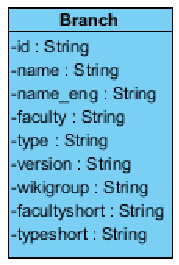
\includegraphics{Branch}
\caption{Branch Objects}
\end{DoxyImage}
 The data structure contains a few elements. For this project, only the following are relevant\+:

\begin{TabularC}{2}
\hline
\rowcolor{lightgray}{\bf Field }&{\bf Description  }\\\cline{1-2}
id &C\+E\+U\+S id of the curriculum. This id is needed for the \hyperlink{index_curr}{curr.php} method. \\\cline{1-2}
name &German name of the curriculum \\\cline{1-2}
namme\+\_\+en &English name of the curriculum \\\cline{1-2}
faculty &Faculty of the curriculum \\\cline{1-2}
type &Bachelor or master studies \\\cline{1-2}
typeshort &Short version of the type ({\itshape B} or {\itshape M}) \\\cline{1-2}
version &Semester when the curriculum was introduced (e.\+g. {\itshape 2013\+W}) \\\cline{1-2}
\end{TabularC}
\hypertarget{index_curr}{}\subsubsection{curr.\+php}\label{index_curr}
\begin{TabularC}{2}
\hline
\rowcolor{lightgray}{\bf Method }&{\bf /curr.php  }\\\cline{1-2}
Input &\char`\"{}authtoken\char`\"{}, \char`\"{}id\char`\"{} \\\cline{1-2}
Output &Object of type curriculum (see below) in J\+S\+O\+N \\\cline{1-2}
\end{TabularC}
The method {\ttfamily curr} returns general information about a curriculum and, more importantly, its structure. A curriculum is identified throug the {\itshape id} returned by \hyperlink{index_list}{list.php} method. Curricula are returned in the following structure\+:


\begin{DoxyImage}
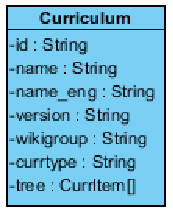
\includegraphics{Curriculum}
\caption{Curriculum Objects}
\end{DoxyImage}
 All but the last element have already been described in \hyperlink{index_list}{list.php} The last one is described below\+:

\begin{TabularC}{2}
\hline
\rowcolor{lightgray}{\bf Field }&{\bf Description  }\\\cline{1-2}
tree &A nested array of {\ttfamily Curr\+Items}, which represents the curriculum structure. The field {\ttfamily id} of each {\ttfamily Curr\+Item} is needed for the \hyperlink{index_detail}{detail.php} method. The field {\ttfamily subtree} contains the subcourses of each course \\\cline{1-2}
\end{TabularC}

\begin{DoxyImage}
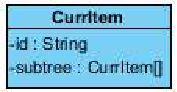
\includegraphics{CurrItem}
\caption{Curr\+Item Objects}
\end{DoxyImage}
 \hypertarget{index_detail}{}\subsubsection{detail.\+php}\label{index_detail}
\begin{TabularC}{2}
\hline
\rowcolor{lightgray}{\bf Method }&{\bf /detail.php  }\\\cline{1-2}
Input &\char`\"{}authtoken\char`\"{}, \char`\"{}id\char`\"{} \mbox{[},\char`\"{}lang\char`\"{}\mbox{]} \\\cline{1-2}
Output &Array of Detail objects (see below) in J\+S\+O\+N \\\cline{1-2}
\end{TabularC}
The method {\ttfamily detail} returns the details for one {\ttfamily Curr\+Item}. A {\ttfamily Curr\+Item} can be a subject (Fach), a module (Modul) or a simple course (Lehrveranstaltung). For localised data the optional parameter {\ttfamily lang} with the value \char`\"{}de\char`\"{} (German) or \char`\"{}en\char`\"{} (English) can be given. Details are returned in the folling data structure\+:


\begin{DoxyImage}
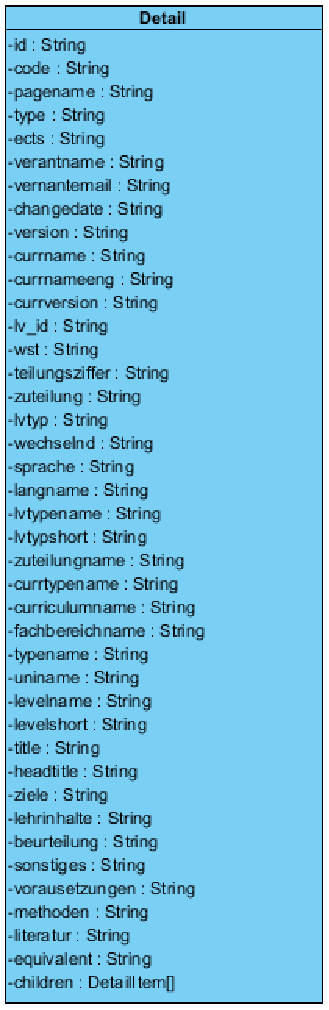
\includegraphics{Detail}
\caption{Detail Objects}
\end{DoxyImage}
 For this project, mainly the following elements are relevant\+:

\begin{TabularC}{2}
\hline
\rowcolor{lightgray}{\bf Field }&{\bf Description  }\\\cline{1-2}
ects &Credits for the course \\\cline{1-2}
verantname &Name of the person responsible for this course \\\cline{1-2}
verantemail &Email of the person responsible for this course \\\cline{1-2}
changedate &Date and time of the last change of this entry (in the format \char`\"{}\+Y\+Y\+Y\+Y-\/\+M\+M-\/\+D\+D hh\+:mm\+:ss\char`\"{}) \\\cline{1-2}
currname &Name of the curriculum that contains this course \\\cline{1-2}
wst &Semester periods per week (Semesterwochenstunden) for this course \\\cline{1-2}
langname &Language the course is held in \\\cline{1-2}
lvtypshort &Short type of the course (e.\+g. V\+L, U\+E, K\+V etc.) \\\cline{1-2}
lvatype &Long type of the course (Vorlesung, Uebung etc.) \\\cline{1-2}
typename &Long type of the entry (subject, module or course) \\\cline{1-2}
type &Number representative of the type of entry (1=subject, 2=module and 3=course) \\\cline{1-2}
title &Course title \\\cline{1-2}
ziele &Course goals \\\cline{1-2}
lehrinhalte &Contents of teaching \\\cline{1-2}
voraussetzungen &Course requirements \\\cline{1-2}
methoden &Teaching methods \\\cline{1-2}
\end{TabularC}
\hypertarget{index_Errors}{}\subsubsection{Errors}\label{index_Errors}
In case of an error, the C\+E\+U\+S A\+P\+I returns a J\+S\+O\+N object with the error message contained in the {\ttfamily error} field. Known errors are\+:
\begin{DoxyItemize}
\item Invalid id given
\item Missing parameter
\item Missing authentication token
\end{DoxyItemize}\hypertarget{index_Modules}{}\subsection{Modules}\label{index_Modules}
\hypertarget{index_CEUS2Drupal}{}\subsubsection{C\+E\+U\+S2\+Drupal}\label{index_CEUS2Drupal}
\hypertarget{index_Import}{}\paragraph{Import}\label{index_Import}
The import of data from C\+E\+U\+S to the Drupal environment is implemented in this component. All its functionality is collected in the \hyperlink{index_CEUS2Drupal}{C\+E\+U\+S2\+Drupal} component. The data model for the Drupal-\/internal representation of courses is defined in the module's \hyperlink{stukowin_8install}{install component}, the necessary database tables are automatically created during the installation. Because the A\+P\+I U\+R\+L and user credentials are prone to change, they need to be configurable. This is achieved in the \hyperlink{group___stukowin___module_ga55d453d5b6f8ae4e643308d8814e67a5}{admin menu}\+:


\begin{DoxyImage}
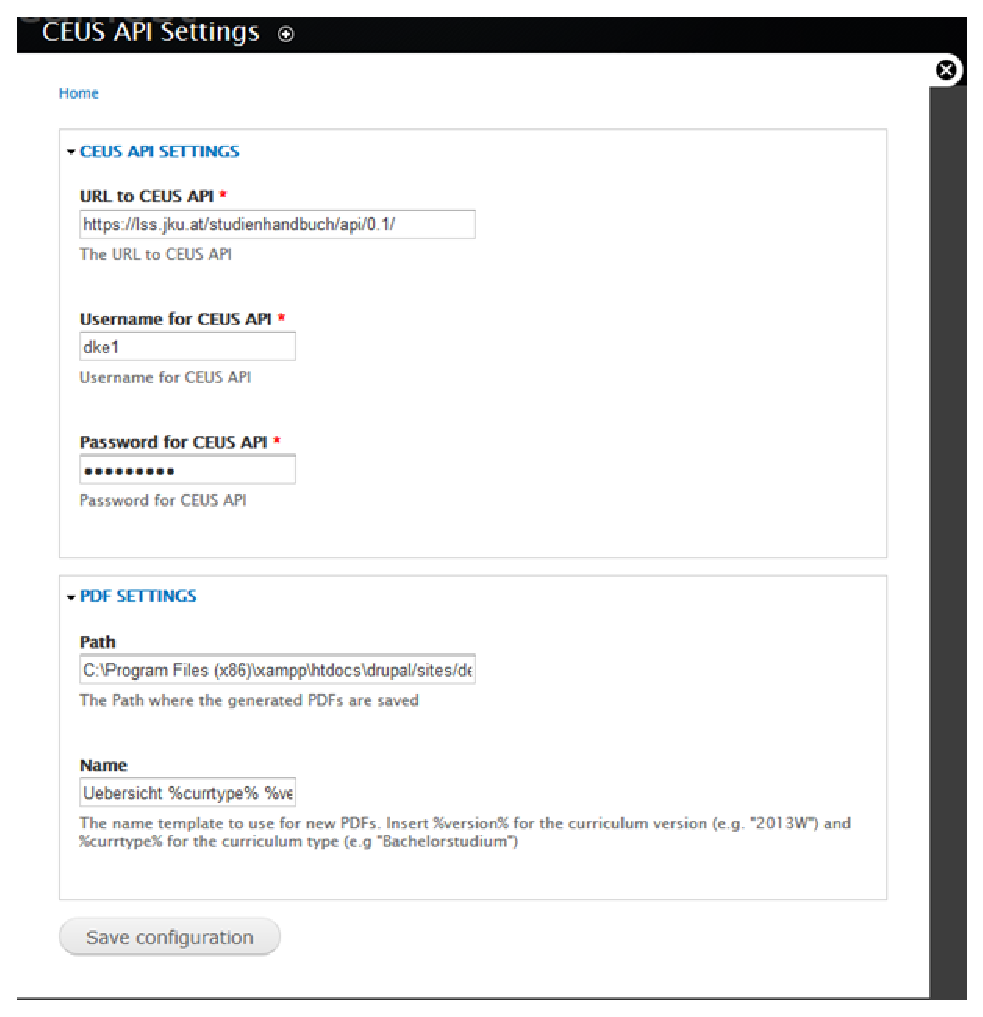
\includegraphics[width=\textwidth]{ModuleConfiguration}
\caption{Module Configuration Page}
\end{DoxyImage}


\begin{DoxyNote}{Note}
Administrator rights are needed to configure the login details
\end{DoxyNote}


 The communication between this module and CEUS occurs as shown in the included \href[pdfnewwindow]{./SequenceDiagramImport.pdf}{SequenceDiagramImport.pdf} file. 

The import from C\+E\+U\+S is performed roughly in the following steps\+:
\begin{DoxyEnumerate}
\item The {\ttfamily auth} token is requested from the C\+E\+U\+S A\+P\+I
\item All available curricula are received from the A\+P\+I
\item For each curriculum, the curriculum tree is requested from the A\+P\+I
\item For each course in the tree, the details are requested in German and English
\item During the first import, new Drupal vocabularies, vocabulary terms and content nodes are created
\item We try our best to parse the field {\ttfamily voraussetzungen} and extract relations between courses (recommended/required)
\end{DoxyEnumerate}

 This process is shown in the included \href[pdfnewwindow]{./FlowchartCEUS2Drupal.pdf}{FlowchartCEUS2Drupal.pdf} file, with the corresponding methods in \hyperlink{classceus__importer}{ceus\+\_\+importer} that perform each step.  Here is a quick textual description of the process\+:

The data import is initiated in the file \hyperlink{stukowin_8module}{stukowin.\+module}. This file first access \hyperlink{classceus__importer_a78572828d11dcdf2a498497d9001d557}{ceus\+\_\+importer\+::connect()} in the file \hyperlink{ceus__importer_8inc_8php}{ceus\+\_\+importer.\+inc.\+php} and prepares the import process. In order for this to work, the necessary settings have to be made in the configuration menu shown above. All methods for the data import are collected in the \hyperlink{ceus__importer_8inc_8php}{ceus\+\_\+importer.\+inc.\+php} file.

After this, the method \hyperlink{classceus__importer_abd2f9a9afc073169b2badcb571cc983c}{ceus\+\_\+importer\+::get\+\_\+curricula()} is called, which starts the import process. It checks if a Drupal vocabulary for the imported curricula already exists. If none are found, a new one is created. If the curricula's version numbers are different, a new vocabulary is created as well.

After getting the tree for each curriculum, the details for its courses are requested and stored.

Another noteworthy part is the method \hyperlink{classceus__importer_a04b7723caf55a2cfd4b92d02754748dc}{ceus\+\_\+importer\+::process\+\_\+relations()}. This method is responsible for parsing the field {\ttfamily voraussetzungen}, which can contain any text possible. The method examines the field in three steps\+:
\begin{DoxyEnumerate}
\item Is the field empty? If not, go to Step 2.
\item Does the field begin with \char`\"{}empfohlen\char`\"{}? If yes, it is a {\itshape recommended} relation, if not it is a {\itshape required} relation.
\item Try to find $<$li$>$ and $<$a$>$ tags and extract a course title or code from them.
\end{DoxyEnumerate}

Requirements are important mostly because they are used and shown in the \hyperlink{index_Drupal2AGG}{automatically generated graphic representation}.

All of the code for the import is contained in the \hyperlink{ceus__importer_8inc_8php}{ceus\+\_\+importer.\+inc.\+php} file.

\begin{DoxySeeAlso}{See also}
\hyperlink{group___c_e_u_s2_drupal}{C\+E\+U\+S2\+Drupal}
\end{DoxySeeAlso}
\hypertarget{index_change_management}{}\paragraph{Change Management}\label{index_change_management}
The functional requirements of this project make it necessary to periodically extract data from C\+E\+U\+S on the one hand and giving administrators and moderators the ability to overwrite data on the other hand. \begin{DoxyRemark}{Remarks}
How to overwrite course data is described in the user documentation.
\end{DoxyRemark}


 This creates the challenge of properly versioning the CMS content, which is why every import follows the rules shown in the included \href[pdfnewwindow]{./Changemanagement.pdf}{Changemanagement.pdf} file 

Every time a content node is created or updated, it gets a red {\itshape New} tag in the content overview (see image below), through which the administrator can easily see which nodes have been updated. In addition to this, the import returns a success message that tells the administrator how many nodes have been created or updated, so that one can easily tell if changes have occurred.


\begin{DoxyImage}
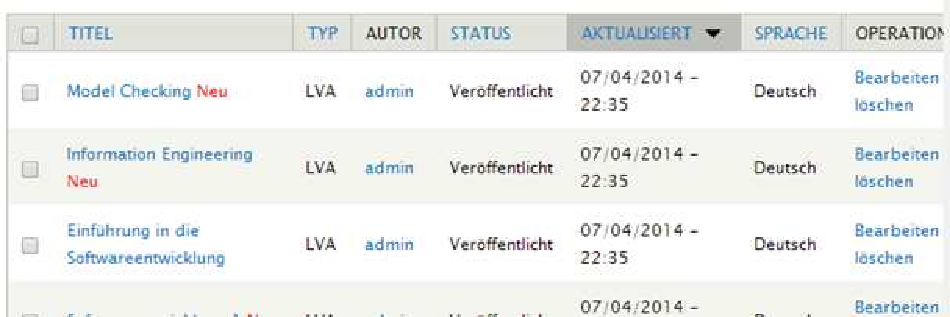
\includegraphics[width=\textwidth]{NewTag}
\caption{Red {\itshape New} Tag}
\end{DoxyImage}
\hypertarget{index_Drupal2ITSV}{}\subsubsection{Drupal2\+I\+T\+S\+V}\label{index_Drupal2ITSV}
As C\+E\+U\+S does not provide any information about fields of specialisation during the master studies and ideal courses of studies, henceforth called I\+T\+S\+V due to its German name, it was a project requirement that new curricula can be created by the administrator for such purposes.

A freely available Drupal module called Taxonomy Manager (\href{https://www.drupal.org/project/taxonomy_manager}{\tt https\+://www.\+drupal.\+org/project/taxonomy\+\_\+manager}) gives the administrator the ability to copy vocabulary terms from one vocabulary to another, which is most of the work. Unfortunately, this process cannot be simplified any further. Nevertheless, we tried to at least automate the task of creating a new vocabulary, copying all of the information over from the source curriculum and creating top-\/level terms (such as \char`\"{}1. Semester\char`\"{} etc.), tasks which will be performed every time a new I\+T\+S\+V or specialisation has to be created.

This component handles exactly that. It inserts a new menu item (at admin/settings/stukowin/taxonomy) where the administrator can select a source curriculum to base the new one on, select whether to create an I\+T\+S\+V or specialisation vocabulary, enter a name and choose how many top-\/level terms should be inserted. Once the administrator has filled out the form, the new vocabulary is automatically created and the browser is redirected to the Taxonomy Manager's \char`\"{}\+Dual View\char`\"{}, where the administrator can begin copying courses into the new vocabulary.

\begin{DoxyRemark}{Remarks}
This component does not have its own file as it does not contain a lot of code. All of its functionality is in the \hyperlink{stukowin_8module}{stukowin.\+module} file.
\end{DoxyRemark}
\begin{DoxySeeAlso}{See also}
\hyperlink{group___drupal2_i_t_s_v}{Drupal2\+I\+T\+S\+V}
\end{DoxySeeAlso}
\hypertarget{index_Drupal2PDF}{}\subsubsection{Drupal2\+P\+D\+F}\label{index_Drupal2PDF}
In order to permanently and easily archive past curricula there is the option to automatically create a course overview P\+D\+F document from the imported courses. For this component to work properly, the necessary settings have to be made in advance (see module configuration image above). The administrator is provided with a new menu (at admin/settings/stukowin/pdf) where the curriculum to be archived can be selected. Once he clicks on \char`\"{}\+Create P\+D\+F\char`\"{}, the P\+D\+F generation in \hyperlink{classoverview_p_d_f_a30ddd92aaf87bca0825c149bd3a7d43f}{overview\+P\+D\+F\+::create\+P\+D\+F()} is started. (All of the P\+D\+F generation code is contained in the \hyperlink{pdf__creator_8inc_8php}{pdf\+\_\+creator.\+inc.\+php} file)



 The PDF generation process will flow as shown in the included \href[pdfnewwindow]{./FlowchartDrupal2PDF.pdf}{FlowchartDrupal2PDF.pdf} file. 

\begin{DoxySeeAlso}{See also}
\hyperlink{group___drupal2_p_d_f}{Drupal2\+P\+D\+F}
\end{DoxySeeAlso}
\hypertarget{index_Drupal2AGG}{}\subsubsection{Drupal2\+A\+G\+G}\label{index_Drupal2AGG}
So far we have described how to import and edit curricula into Drupal. But part of the functional requirements were also being able to automatically display the curricula on the website in the form of an automatically generated graphic (A\+G\+G). This component provides the functionality for doing exactly that. Again, it can be separated into three components\+:\hypertarget{index_json}{}\paragraph{Drupal J\+S\+O\+N Interface}\label{index_json}
To make the curricula data available to clients, several J\+S\+O\+N interfaces have been implemented that make curricula publicly reachable. This is needed so that the client browser can properly display the curricula.

The following interfaces are available\+: \begin{TabularC}{4}
\hline
\rowcolor{lightgray}{\bf Name }&{\bf Path }&{\bf Input Parameter }&{\bf Description  }\\\cline{1-4}
Curriculum List &stukowin/crclmlst &\char`\"{}currtype\char`\"{} \+: Type of curriculum to get (\char`\"{}\+Bachelorstudium\char`\"{} or \char`\"{}\+Masterstudium\char`\"{})~\newline
\char`\"{}taxtypes\char`\"{} \+: Types of vocabularies to get (\char`\"{}curriculum\char`\"{}, \char`\"{}itsv\char`\"{} and/or \char`\"{}specialisation\char`\"{}) &Returns a list of all curricula currently published (weight $<$ 0), like \hyperlink{index_list}{list.\+php} \\\cline{1-4}
Curriculum Tree &stukowin/crclm &Vocabulary id of the curriculum to get &Returns the curriculum tree of one curriculum, containing all courses and their details \\\cline{1-4}
Single course &stukowin/lva &Node id of the course to get &Returns the details of a single course \\\cline{1-4}
\end{TabularC}
All of these interfaces are defined in the \hyperlink{stukowin_8module}{stukowin.\+module} file.\hypertarget{index_plugin}{}\paragraph{C\+K\+Editor Plug-\/in}\label{index_plugin}
As the dynamic display of curricula in the browser requires a strict H\+T\+M\+L document structure, we refrained from letting the administrator insert the code himself wherever a curriculum display was needed and instead implemented a plug-\/in for the C\+K\+Editor (\href{https://www.drupal.org/project/ckeditor}{\tt https\+://www.\+drupal.\+org/project/ckeditor}) which inserts the code automatically on the click of a button. The plug-\/in is registered with drupal in the \hyperlink{group___drupal2_a_g_g_gae3c906d1ab9c3d8ed245d58c1ebf2a4a}{stukowin\+\_\+ckeditor\+\_\+plugin()} method. It is then defined in the \hyperlink{plugin_8js}{plugin.\+js} file and the dialog for inserting a curriculum view is defined in the \hyperlink{stukowin__curriculum_8js}{stukowin\+\_\+curriculum.\+js} file.

\begin{DoxyNote}{Note}
In order for this plug-\/in to work properly, some settings have to be made in the C\+K\+Editor. This is described in the operator manual.
\end{DoxyNote}
\hypertarget{index_graph}{}\paragraph{Graph.\+js}\label{index_graph}
The main task of displaying the curricula in the client's browser is performed by this file. It fetches the data from the J\+S\+O\+N interfaces described \hyperlink{index_json}{above} and creates the D\+O\+M elements in the browser. It also registers click handlers for things such as expanding/reducing a course, showing prerequisites and selecting a different curriculum. \begin{DoxyNote}{Note}
The display layout is configured in the curriculum\+\_\+stlye.\+css file (not included in this documentation)
\end{DoxyNote}
As an example, the output could look like this\+:


\begin{DoxyImage}
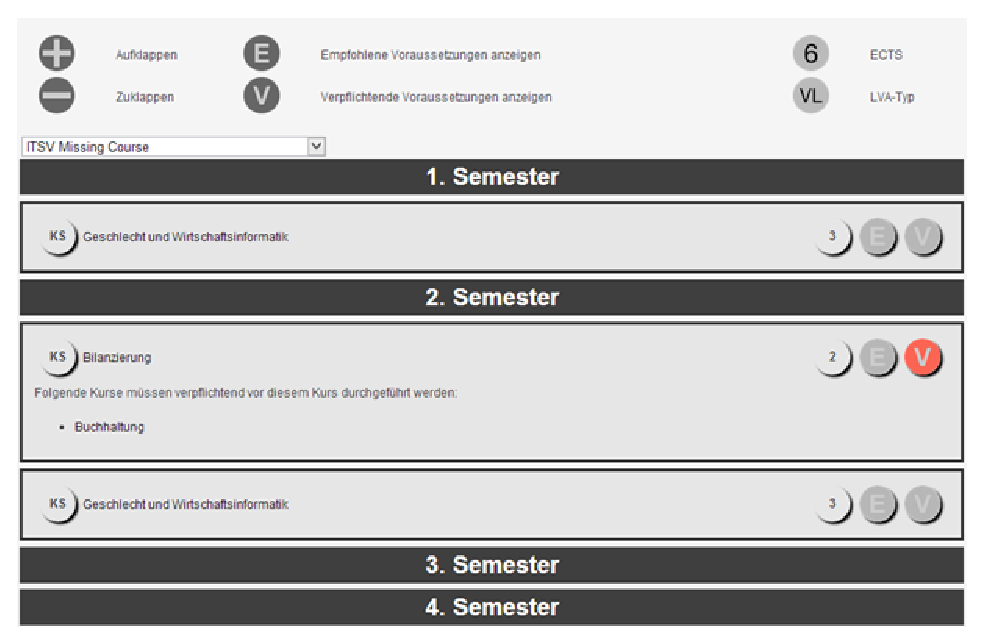
\includegraphics[width=\textwidth]{Drupal2AGG}
\caption{Graphical Representation}
\end{DoxyImage}


\begin{DoxySeeAlso}{See also}
\hyperlink{group___drupal2_a_g_g}{Drupal2\+A\+G\+G}
\end{DoxySeeAlso}
\hypertarget{index_Other}{}\subsubsection{Other}\label{index_Other}
All of the components described above need to work together somehow and at the same time be accessible to Drupal itself. For this reason there are several methods and files to ensure a smooth cooperation, some of which are worth mentioning explicitly\+:
\begin{DoxyItemize}
\item The \hyperlink{classcontent__manager}{content\+\_\+manager} class is responsible for accessing the imported curricula data
\item The \hyperlink{stukowin_8install}{stukowin.\+install} file is responsible for installing and uninstalling the module and all the data structures that come with it
\item The \hyperlink{group___stukowin___module_ga59cfbad113b7aa2d10f0b204a5f7ba0d}{stukowin\+\_\+menu()} function sets up all the callback U\+R\+Ls
\item The \hyperlink{group___stukowin___module_ga55d453d5b6f8ae4e643308d8814e67a5}{stukowin\+\_\+admin()} function is responsible for the configuration menu
\item The stukowin.\+info file contains all meta information about the module
\end{DoxyItemize}\hypertarget{index_Development}{}\subsection{Development}\label{index_Development}
\hypertarget{index_Authors}{}\subsubsection{Authors}\label{index_Authors}
\begin{DoxyNote}{Note}
Every file, class, method and member is documented with an {\ttfamily @author} tag. The person tagged as {\ttfamily @author} (thus being shown as the author) is the main/initial author of that file, class, method or member. 

All other authors, (people that have helped during initial development, fixed bugs or made changes) are tagged with the {\ttfamily @author{\bfseries s} }(plural) tag, thus being shown under Author{\bfseries s(plural)}. 

If a file, class, method or member has been authored by multiple people equally, all of them are tagged with the {\ttfamily @author{\bfseries s} tag} and there is no {\ttfamily @author}. 

If you have any questions regarding the system, feel free to contact the respective author.
\end{DoxyNote}
The following list shows an overview of every person that has participated in writing this module, with a quick summary of what they have mostly contributed to\+:
\begin{DoxyItemize}
\item {\bfseries Jakob Strasser} -\/ \href{mailto:jakob.strasser@telenet.be}{\tt jakob.\+strasser@telenet.\+be} ~\newline
Main author of the \hyperlink{index_CEUS2Drupal}{P\+D\+F generation component} and the \hyperlink{graph_8js}{graph.\+js} file. Participating author in most files/components. 


\item {\bfseries Konstantinos Dafalias} -\/ \href{mailto:kdafalias@gmail.com}{\tt kdafalias@gmail.\+com} ~\newline
Mostly responsible for the \hyperlink{index_CEUS2Drupal}{C\+E\+U\+S import} and the \hyperlink{group___stukowin___module}{Module Core} 


\item {\bfseries Werner Breuer} -\/ \href{mailto:bluescreenwerner@gmail.com}{\tt bluescreenwerner@gmail.\+com} ~\newline
Co-\/author of the \hyperlink{index_plugin}{C\+K\+Editor Plug-\/in} and the \hyperlink{index_Drupal2AGG}{Drupal2\+A\+G\+G} component in general, as well as the \hyperlink{index_Drupal2ITSV}{Drupal2\+I\+T\+S\+V} component. Participated in a lot of debugging. 


\item {\bfseries Markus Gutmayer} -\/ \href{mailto:m.gutmayer@gmail.com}{\tt m.\+gutmayer@gmail.\+com} ~\newline
Co-\/author of the \hyperlink{index_plugin}{C\+K\+Editor Plug-\/in} and the \hyperlink{index_Drupal2AGG}{Drupal2\+A\+G\+G} component in general, as well as the \hyperlink{index_Drupal2ITSV}{Drupal2\+I\+T\+S\+V} component. Participated in a lot of debugging. 


\item {\bfseries Fabian Puehringer} -\/ \href{mailto:f.puehringer@24speed.at}{\tt f.\+puehringer@24speed.\+at} ~\newline
Assistance with \hyperlink{index_Drupal2PDF}{Drupal2\+P\+D\+F} and \hyperlink{index_Drupal2AGG}{Drupal2\+A\+G\+G} 


\item {\bfseries Manuel Muehlburger} -\/ \href{mailto:Hansbert92@googlemail.com}{\tt Hansbert92@googlemail.\+com} ~\newline
Layout and design for the \hyperlink{index_Drupal2AGG}{Drupal2\+A\+G\+G} component (mainly the \hyperlink{index_graph}{Graph.\+js})
\end{DoxyItemize}\hypertarget{index_versionnumbers}{}\subsubsection{Version Numbers}\label{index_versionnumbers}
Every file and class has a version number, composed of four parts\+: {\itshape major.\+minor.\+revision} {\itshape date} 
\begin{DoxyItemize}
\item {\itshape Major} signifies a major release, such as the initial release
\item {\itshape Minor} signifies the addition of a new feature
\item {\itshape Revision} signifies a bug fix or something similarly small
\item {\itshape Date} shows when the last change was made to the source code (in the format \char`\"{}\+Y\+Y\+Y\+Y-\/\+M\+M-\/\+D\+D\char`\"{})
\end{DoxyItemize}\hypertarget{index_versioncontrol}{}\subsubsection{Version Control}\label{index_versioncontrol}
When the project started, there were two groups, each of which used a different version control system. Group 1 used S\+V\+N on \href{http://cloudforge.com}{\tt http\+://cloudforge.\+com} while group 2 used \href{http://bitbucket.org}{\tt http\+://bitbucket.\+org}. When the two groups were merged, the S\+V\+N repository was dropped. Due to privilege problems with bitbucket, it was decided to move the entire repository to \href{http://github.com}{\tt http\+://github.\+com}, as everyone had access there. At the time writing this documentation, the repository is available at \href{http://github.com/TheJake123/DrupalModul}{\tt http\+://github.\+com/\+The\+Jake123/\+Drupal\+Modul}.

As the repository is open source, the commit, issue and change history can be publicly viewed. Additionally, every file, class, method and member has been documented with a {\ttfamily @since} tag with the following format\+: \char`\"{}\+Commit $<$hash$>$ on Y\+Y\+Y\+Y-\/\+M\+M-\/\+D\+D\char`\"{}, so that it is easily visible when a file, class, method or member has been added.\hypertarget{index_Included}{}\subsection{Included Libraries/\+Files}\label{index_Included}
For the P\+D\+F generation, the free and open source library \href{http://www.tcpdf.org/}{\tt T\+C\+P\+D\+F} is used and included in the project.

For parsing course relationships, the \href{http://simplehtmldom.sourceforge.net/}{\tt simple\+\_\+html\+\_\+dom.\+php} file is used 
\section{Module Index}
\subsection{Modules}
Here is a list of all modules\+:\begin{DoxyCompactList}
\item \contentsline{section}{C\+E\+U\+S2\+Drupal}{\pageref{group___c_e_u_s2_drupal}}{}
\item \contentsline{section}{Drupal2\+A\+G\+G}{\pageref{group___drupal2_a_g_g}}{}
\item \contentsline{section}{Drupal2\+P\+D\+F}{\pageref{group___drupal2_p_d_f}}{}
\item \contentsline{section}{Module Core}{\pageref{group___stukowin___module}}{}
\item \contentsline{section}{Drupal2\+I\+T\+S\+V}{\pageref{group___drupal2_i_t_s_v}}{}
\end{DoxyCompactList}

\section{Hierarchical Index}
\subsection{Class Hierarchy}
This inheritance list is sorted roughly, but not completely, alphabetically\+:\begin{DoxyCompactList}
\item \contentsline{section}{ceus\+\_\+importer}{\pageref{classceus__importer}}{}
\item \contentsline{section}{content\+\_\+manager}{\pageref{classcontent__manager}}{}
\item \contentsline{section}{E\+X\+S\+T\+Y\+P\+E}{\pageref{union_e_x_s_t_y_p_e}}{}
\item \contentsline{section}{T\+C\+P\+D\+F}{\pageref{class_t_c_p_d_f}}{}
\begin{DoxyCompactList}
\item \contentsline{section}{overview\+P\+D\+F}{\pageref{classoverview_p_d_f}}{}
\end{DoxyCompactList}
\end{DoxyCompactList}

\section{Data Structure Index}
\subsection{Data Structures}
Here are the data structures with brief descriptions\+:\begin{DoxyCompactList}
\item\contentsline{section}{\hyperlink{classceus__importer}{ceus\+\_\+importer} \\*Imports data from C\+E\+U\+S and stores it in the Drupal database }{\pageref{classceus__importer}}{}
\item\contentsline{section}{\hyperlink{classcontent__manager}{content\+\_\+manager} \\*Access to drupal vocabularies and content nodes }{\pageref{classcontent__manager}}{}
\item\contentsline{section}{\hyperlink{union_e_x_s_t_y_p_e}{E\+X\+S\+T\+Y\+P\+E} }{\pageref{union_e_x_s_t_y_p_e}}{}
\item\contentsline{section}{\hyperlink{classoverview_p_d_f}{overview\+P\+D\+F} \\*Class for P\+D\+F document generation from curricula data }{\pageref{classoverview_p_d_f}}{}
\item\contentsline{section}{\hyperlink{class_t_c_p_d_f}{T\+C\+P\+D\+F} }{\pageref{class_t_c_p_d_f}}{}
\end{DoxyCompactList}

\section{File Index}
\subsection{File List}
Here is a list of all files with brief descriptions\+:\begin{DoxyCompactList}
\item\contentsline{section}{\hyperlink{ceus__importer_8inc_8php}{ceus\+\_\+importer.\+inc.\+php} \\*Imports data from C\+E\+U\+S }{\pageref{ceus__importer_8inc_8php}}{}
\item\contentsline{section}{\hyperlink{content__manager_8inc_8php}{content\+\_\+manager.\+inc.\+php} \\*Access to curricula data }{\pageref{content__manager_8inc_8php}}{}
\item\contentsline{section}{\hyperlink{graph_8js}{graph.\+js} \\*Script for nicely displaying C\+E\+U\+S data }{\pageref{graph_8js}}{}
\item\contentsline{section}{\hyperlink{pdf__creator_8inc_8php}{pdf\+\_\+creator.\+inc.\+php} \\*P\+D\+F document generation from curricula data }{\pageref{pdf__creator_8inc_8php}}{}
\item\contentsline{section}{\hyperlink{plugin_8js}{plugin.\+js} \\*Registers the C\+K\+Editor plugin }{\pageref{plugin_8js}}{}
\item\contentsline{section}{\hyperlink{stukowin_8install}{stukowin.\+install} \\*Install script }{\pageref{stukowin_8install}}{}
\item\contentsline{section}{\hyperlink{stukowin_8module}{stukowin.\+module} \\*Main module file }{\pageref{stukowin_8module}}{}
\item\contentsline{section}{\hyperlink{stukowin__curriculum_8js}{stukowin\+\_\+curriculum.\+js} \\*The stukowin\+\_\+curriculum dialog definition }{\pageref{stukowin__curriculum_8js}}{}
\end{DoxyCompactList}

\section{Module Documentation}
\hypertarget{group___c_e_u_s2_drupal}{\subsection{C\+E\+U\+S2\+Drupal}
\label{group___c_e_u_s2_drupal}\index{C\+E\+U\+S2\+Drupal@{C\+E\+U\+S2\+Drupal}}
}


Module for importing data from C\+E\+U\+S.  


\subsubsection*{Files}
\begin{DoxyCompactItemize}
\item 
file \hyperlink{ceus__importer_8inc_8php}{ceus\+\_\+importer.\+inc.\+php}
\begin{DoxyCompactList}\small\item\em Imports data from C\+E\+U\+S. \end{DoxyCompactList}\end{DoxyCompactItemize}
\subsubsection*{Data Structures}
\begin{DoxyCompactItemize}
\item 
class \hyperlink{classceus__importer}{ceus\+\_\+importer}
\begin{DoxyCompactList}\small\item\em Imports data from C\+E\+U\+S and stores it in the Drupal database. \end{DoxyCompactList}\end{DoxyCompactItemize}
\subsubsection*{Functions}
\begin{DoxyCompactItemize}
\item 
\hyperlink{group___c_e_u_s2_drupal_ga481789ce9904fc10aefb8eaf7534133b}{stukowin\+\_\+pre\+\_\+retreive} (\$form, \&\$form\+\_\+state)
\begin{DoxyCompactList}\small\item\em Menu callback for import (\char`\"{}admin/settings/stukowin/import\char`\"{}) \end{DoxyCompactList}\item 
\hyperlink{group___c_e_u_s2_drupal_ga433b18d1cf617b28cca3fc0dd47d8062}{stukowin\+\_\+pre\+\_\+retreive\+\_\+submit} (\$form, \&\$form\+\_\+state)
\begin{DoxyCompactList}\small\item\em Submit handler for \hyperlink{group___c_e_u_s2_drupal_ga481789ce9904fc10aefb8eaf7534133b}{stukowin\+\_\+pre\+\_\+retreive()} \end{DoxyCompactList}\end{DoxyCompactItemize}


\subsubsection{Detailed Description}
Module for importing data from C\+E\+U\+S. 

This module is reponsible for requesting the data from the C\+E\+U\+S A\+P\+I and storing it in the drupal database. It also implements the functions for the change management.

For a more detailed description see \hyperlink{index_CEUS2Drupal}{C\+E\+U\+S2\+Drupal}

\begin{DoxyAuthor}{Author}
Konstantinos Dafalias -\/ \href{mailto:kdafalias@gmail.com}{\tt kdafalias@gmail.\+com} 
\end{DoxyAuthor}
\begin{DoxyAuthor}{Authors}
Jakob Strasser -\/ \href{mailto:jakob.strasser@telenet.be}{\tt jakob.\+strasser@telenet.\+be} 

Markus Gutmayer -\/ \href{mailto:m.gutmayer@gmail.com}{\tt m.\+gutmayer@gmail.\+com} 

Werner Breuer -\/ \href{mailto:bluescreenwerner@gmail.com}{\tt bluescreenwerner@gmail.\+com} 
\end{DoxyAuthor}


\subsubsection{Function Documentation}
\hypertarget{group___c_e_u_s2_drupal_ga481789ce9904fc10aefb8eaf7534133b}{\index{C\+E\+U\+S2\+Drupal@{C\+E\+U\+S2\+Drupal}!stukowin\+\_\+pre\+\_\+retreive@{stukowin\+\_\+pre\+\_\+retreive}}
\index{stukowin\+\_\+pre\+\_\+retreive@{stukowin\+\_\+pre\+\_\+retreive}!C\+E\+U\+S2\+Drupal@{C\+E\+U\+S2\+Drupal}}
\paragraph[{stukowin\+\_\+pre\+\_\+retreive}]{\setlength{\rightskip}{0pt plus 5cm}stukowin\+\_\+pre\+\_\+retreive (
\begin{DoxyParamCaption}
\item[{}]{\$form, }
\item[{\&}]{\$form\+\_\+state}
\end{DoxyParamCaption}
)}}\label{group___c_e_u_s2_drupal_ga481789ce9904fc10aefb8eaf7534133b}


Menu callback for import (\char`\"{}admin/settings/stukowin/import\char`\"{}) 

Used as a warning before starting the import, as the process usually takes a long time to complete.

\begin{DoxyRemark}{Remarks}
There is nothing to do in this menu except click \char`\"{}\+Ok\char`\"{}.
\end{DoxyRemark}

\begin{DoxyParams}[1]{Parameters}
array & {\em \$form} & Form structure as given by Drupal \\
\hline
array & {\em \$form\+\_\+state} & Form state as given by Drupal \\
\hline
\end{DoxyParams}
\begin{DoxyReturn}{Returns}
The filled out form structure
\end{DoxyReturn}
\begin{DoxyAuthor}{Author}
Jakob Strasser -\/ \href{mailto:jakob.strasser@telenet.be}{\tt jakob.\+strasser@telenet.\+be} 
\end{DoxyAuthor}
\begin{DoxyVersion}{Version}
1.\+1.\+0 2014-\/07-\/31 
\end{DoxyVersion}
\begin{DoxySince}{Since}
Commit \href{http://github.com/TheJake123/DrupalModul/commit/bcdb4bad5d0a81dbf12a98c54f8512035a8661d4}{\tt bcdb4ba} on 2014-\/06-\/30
\end{DoxySince}
\begin{DoxySeeAlso}{See also}
stukowin\+\_\+re\+\_\+retrieve\+\_\+submit() 
\end{DoxySeeAlso}


Definition at line 247 of file stukowin.\+module.

\hypertarget{group___c_e_u_s2_drupal_ga433b18d1cf617b28cca3fc0dd47d8062}{\index{C\+E\+U\+S2\+Drupal@{C\+E\+U\+S2\+Drupal}!stukowin\+\_\+pre\+\_\+retreive\+\_\+submit@{stukowin\+\_\+pre\+\_\+retreive\+\_\+submit}}
\index{stukowin\+\_\+pre\+\_\+retreive\+\_\+submit@{stukowin\+\_\+pre\+\_\+retreive\+\_\+submit}!C\+E\+U\+S2\+Drupal@{C\+E\+U\+S2\+Drupal}}
\paragraph[{stukowin\+\_\+pre\+\_\+retreive\+\_\+submit}]{\setlength{\rightskip}{0pt plus 5cm}stukowin\+\_\+pre\+\_\+retreive\+\_\+submit (
\begin{DoxyParamCaption}
\item[{}]{\$form, }
\item[{\&}]{\$form\+\_\+state}
\end{DoxyParamCaption}
)}}\label{group___c_e_u_s2_drupal_ga433b18d1cf617b28cca3fc0dd47d8062}


Submit handler for \hyperlink{group___c_e_u_s2_drupal_ga481789ce9904fc10aefb8eaf7534133b}{stukowin\+\_\+pre\+\_\+retreive()} 

Starts the import process and displays the outcome to the user.


\begin{DoxyParams}[1]{Parameters}
array & {\em \$form} & Form structure as given by Drupal \\
\hline
array & {\em \$form\+\_\+state} & Form state as given by Drupal\\
\hline
\end{DoxyParams}
\begin{DoxyAuthor}{Author}
Jakob Strasser -\/ \href{mailto:jakob.strasser@telenet.be}{\tt jakob.\+strasser@telenet.\+be} 
\end{DoxyAuthor}
\begin{DoxyVersion}{Version}
1.\+0.\+0 2014-\/07-\/16 
\end{DoxyVersion}
\begin{DoxySince}{Since}
Commit \href{http://github.com/TheJake123/DrupalModul/commit/bcdb4bad5d0a81dbf12a98c54f8512035a8661d4}{\tt bcdb4ba} on 2014-\/06-\/30
\end{DoxySince}
\begin{DoxySeeAlso}{See also}
\hyperlink{group___c_e_u_s2_drupal_ga481789ce9904fc10aefb8eaf7534133b}{stukowin\+\_\+pre\+\_\+retreive()} 
\end{DoxySeeAlso}


Definition at line 287 of file stukowin.\+module.


\hypertarget{group___drupal2_a_g_g}{\subsection{Drupal2\+A\+G\+G}
\label{group___drupal2_a_g_g}\index{Drupal2\+A\+G\+G@{Drupal2\+A\+G\+G}}
}


Module for transforming C\+E\+U\+S data to a proper graphical representation.  


\subsubsection*{Files}
\begin{DoxyCompactItemize}
\item 
file \hyperlink{graph_8js}{graph.\+js}
\begin{DoxyCompactList}\small\item\em Script for nicely displaying C\+E\+U\+S data. \end{DoxyCompactList}\item 
file \hyperlink{stukowin__curriculum_8js}{stukowin\+\_\+curriculum.\+js}
\begin{DoxyCompactList}\small\item\em The stukowin\+\_\+curriculum dialog definition. \end{DoxyCompactList}\item 
file \hyperlink{plugin_8js}{plugin.\+js}
\begin{DoxyCompactList}\small\item\em Registers the C\+K\+Editor plugin. \end{DoxyCompactList}\end{DoxyCompactItemize}
\subsubsection*{Functions}
\begin{DoxyCompactItemize}
\item 
\hyperlink{group___drupal2_a_g_g_gaf137f10bef98707dacaf33d6581773d0}{stukowin\+\_\+get\+\_\+crclm\+\_\+taxonomy} (\$i\+V\+I\+D)
\begin{DoxyCompactList}\small\item\em J\+S\+O\+N service for the nested array of courses details for one curriculum. \end{DoxyCompactList}\item 
\hyperlink{group___drupal2_a_g_g_gad0cb4d7faa68097f5b7df8311e36b22e}{stukowin\+\_\+get\+\_\+crclm\+\_\+list} ()
\begin{DoxyCompactList}\small\item\em J\+S\+O\+N service for a list of all currently published curricula. \end{DoxyCompactList}\item 
\hyperlink{group___drupal2_a_g_g_ga7522e206f1a87971b916a7a0be0098c6}{stukowin\+\_\+get\+\_\+lva} (\$i\+Node\+I\+D)
\begin{DoxyCompactList}\small\item\em J\+S\+O\+N service for the details of a single course. \end{DoxyCompactList}\item 
\hyperlink{group___drupal2_a_g_g_gae3c906d1ab9c3d8ed245d58c1ebf2a4a}{stukowin\+\_\+ckeditor\+\_\+plugin} ()
\begin{DoxyCompactList}\small\item\em implements hook\+\_\+ckeditor\+\_\+plugin \end{DoxyCompactList}\item 
\hyperlink{group___drupal2_a_g_g_ga3bf2203298453c41bf9a5ec48d3c2de3}{stukowin\+\_\+theme\+\_\+registry\+\_\+alter} (\&\$theme\+\_\+registry)
\begin{DoxyCompactList}\small\item\em implements hook\+\_\+theme\+\_\+registry\+\_\+alter \end{DoxyCompactList}\end{DoxyCompactItemize}


\subsubsection{Detailed Description}
Module for transforming C\+E\+U\+S data to a proper graphical representation. 

This module contains all files, classes and methods that provide the functionality for automatically generating a visual representation of the imported curricula data.\hypertarget{group___drupal2_a_g_g_aggjson}{}\subsubsection{Drupal J\+S\+O\+N Interface}\label{group___drupal2_a_g_g_aggjson}
To make the curricula data available to clients, several J\+S\+O\+N interfaces have been implemented that make curricula publicly reachable. This is needed so that the client browser can properly display the curricula.

The following interfaces are available\+: \begin{TabularC}{4}
\hline
\rowcolor{lightgray}{\bf Name }&{\bf Path }&{\bf Input Parameter }&{\bf Description  }\\\cline{1-4}
Curriculum List &stukowin/crclmlst &\char`\"{}currtype\char`\"{} \+: Type of curriculum to get (\char`\"{}\+Bachelorstudium\char`\"{} or \char`\"{}\+Masterstudium\char`\"{})~\newline
\char`\"{}taxtypes\char`\"{} \+: Types of vocabularies to get (\char`\"{}curriculum\char`\"{}, \char`\"{}itsv\char`\"{} and/or \char`\"{}specialisation\char`\"{}) &Returns a list of all curricula currently published (weight $<$ 0), like \hyperlink{index_list}{list.\+php} \\\cline{1-4}
Curriculum Tree &stukowin/crclm &Vocabulary id of the curriculum to get &Returns the curriculum tree of one curriculum, containing all courses and their details \\\cline{1-4}
Single course &stukowin/lva &Node id of the course to get &Returns the details of a single course \\\cline{1-4}
\end{TabularC}
All of these interfaces are defined in the \hyperlink{stukowin_8module}{stukowin.\+module} file.\hypertarget{group___drupal2_a_g_g_aggplugin}{}\subsubsection{C\+K\+Editor Plug-\/in}\label{group___drupal2_a_g_g_aggplugin}
As the dynamic display of curricula in the browser requires a strict H\+T\+M\+L document structure, we refrained from letting the administrator insert the code himself wherever a curriculum display was needed and instead implemented a plug-\/in for the C\+K\+Editor (\href{https://www.drupal.org/project/ckeditor}{\tt https\+://www.\+drupal.\+org/project/ckeditor}) which inserts the code automatically on the click of a button. The plug-\/in is registered with drupal in the \hyperlink{group___drupal2_a_g_g_gae3c906d1ab9c3d8ed245d58c1ebf2a4a}{stukowin\+\_\+ckeditor\+\_\+plugin()} method. It is then defined in the \hyperlink{plugin_8js}{plugin.\+js} file and the dialog for inserting a curriculum view is defined in the \hyperlink{stukowin__curriculum_8js}{stukowin\+\_\+curriculum.\+js} file.

\begin{DoxyNote}{Note}
In order for this plug-\/in to work properly, some settings have to be made in the C\+K\+Editor. This is described in the operator manual.
\end{DoxyNote}
\hypertarget{group___drupal2_a_g_g_agggraph}{}\subsubsection{Graph.\+js}\label{group___drupal2_a_g_g_agggraph}
The main task of displaying the curricula in the client's browser is performed by this file. It fetches the data from the J\+S\+O\+N interfaces described \hyperlink{index_json}{above} and creates the D\+O\+M elements in the browser. It also registers click handlers for things such as expanding/reducing a course, showing prerequisites and selecting a different curriculum. \begin{DoxyNote}{Note}
The display layout is configured in the curriculum\+\_\+stlye.\+css file (not included in this documentation)
\end{DoxyNote}
As an example, the output could look like this\+:


\begin{DoxyImage}
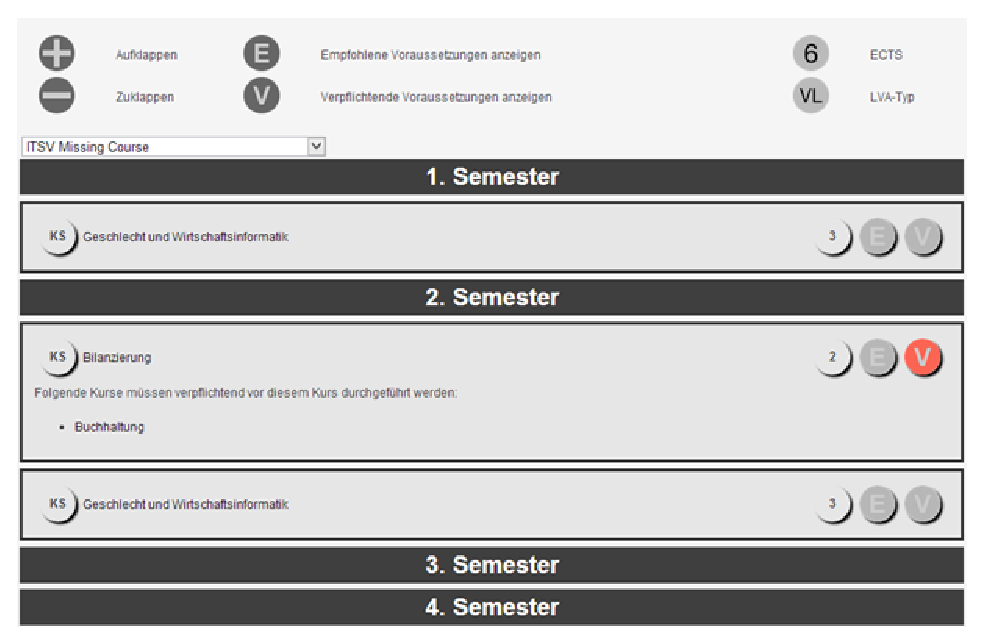
\includegraphics[width=\textwidth]{Drupal2AGG}
\caption{Graphical Representation}
\end{DoxyImage}


\begin{DoxyAuthor}{Authors}
Jakob Strasser -\/ \href{mailto:jakob.strasser@telenet.be}{\tt jakob.\+strasser@telenet.\+be} 

Markus Gutmayer -\/ \href{mailto:m.gutmayer@gmail.com}{\tt m.\+gutmayer@gmail.\+com} 

Werner Breuer -\/ \href{mailto:bluescreenwerner@gmail.com}{\tt bluescreenwerner@gmail.\+com} 

Manuel Muehlburger -\/ \href{mailto:Hansbert92@googlemail.com}{\tt Hansbert92@googlemail.\+com} 
\end{DoxyAuthor}


\subsubsection{Function Documentation}
\hypertarget{group___drupal2_a_g_g_gae3c906d1ab9c3d8ed245d58c1ebf2a4a}{\index{Drupal2\+A\+G\+G@{Drupal2\+A\+G\+G}!stukowin\+\_\+ckeditor\+\_\+plugin@{stukowin\+\_\+ckeditor\+\_\+plugin}}
\index{stukowin\+\_\+ckeditor\+\_\+plugin@{stukowin\+\_\+ckeditor\+\_\+plugin}!Drupal2\+A\+G\+G@{Drupal2\+A\+G\+G}}
\paragraph[{stukowin\+\_\+ckeditor\+\_\+plugin}]{\setlength{\rightskip}{0pt plus 5cm}stukowin\+\_\+ckeditor\+\_\+plugin (
\begin{DoxyParamCaption}
{}
\end{DoxyParamCaption}
)}}\label{group___drupal2_a_g_g_gae3c906d1ab9c3d8ed245d58c1ebf2a4a}


implements hook\+\_\+ckeditor\+\_\+plugin 

Adds the hook for the \hyperlink{stukowin__curriculum_8js}{ckeditor plugin} to insert a curriculum display.

\begin{DoxyAuthor}{Authors}
Werner Breuer -\/ \href{mailto:bluescreenwerner@gmail.com}{\tt bluescreenwerner@gmail.\+com} 

Markus Gutmayer -\/ \href{mailto:m.gutmayer@gmail.com}{\tt m.\+gutmayer@gmail.\+com} 
\end{DoxyAuthor}
\begin{DoxyVersion}{Version}
1.\+0.\+0 2014-\/07-\/16 
\end{DoxyVersion}
\begin{DoxySince}{Since}
Commit \href{http://github.com/TheJake123/DrupalModul/commit/b63de89ea0d0b45b428d333a4ba5c8d859047ba2}{\tt b63de89} on 2014-\/07-\/01 
\end{DoxySince}


Definition at line 599 of file stukowin.\+module.

\hypertarget{group___drupal2_a_g_g_gad0cb4d7faa68097f5b7df8311e36b22e}{\index{Drupal2\+A\+G\+G@{Drupal2\+A\+G\+G}!stukowin\+\_\+get\+\_\+crclm\+\_\+list@{stukowin\+\_\+get\+\_\+crclm\+\_\+list}}
\index{stukowin\+\_\+get\+\_\+crclm\+\_\+list@{stukowin\+\_\+get\+\_\+crclm\+\_\+list}!Drupal2\+A\+G\+G@{Drupal2\+A\+G\+G}}
\paragraph[{stukowin\+\_\+get\+\_\+crclm\+\_\+list}]{\setlength{\rightskip}{0pt plus 5cm}stukowin\+\_\+get\+\_\+crclm\+\_\+list (
\begin{DoxyParamCaption}
{}
\end{DoxyParamCaption}
)}}\label{group___drupal2_a_g_g_gad0cb4d7faa68097f5b7df8311e36b22e}


J\+S\+O\+N service for a list of all currently published curricula. 

The type of curriculum (e.\+g. \char`\"{}\+Bachelorstudium\char`\"{}, \char`\"{}\+Masterstudium\char`\"{}), types of taxonomies (e.\+g. \char`\"{}curriculum\char`\"{}, \char`\"{}itsv\char`\"{} or \char`\"{}specialisation\char`\"{}) and the language (e.\+g. \char`\"{}de\char`\"{}) can be given as H\+T\+T\+P G\+E\+T parameters through the respective parameter names {\ttfamily \char`\"{}currtype\char`\"{}}, {\ttfamily taxtypes} and {\ttfamily lang}.

\begin{DoxyAuthor}{Authors}
Konstantinos Dafalias -\/ \href{mailto:kdafalias@gmail.com}{\tt kdafalias@gmail.\+com} 

Jakob Strasser -\/ \href{mailto:jakob.strasser@telenet.be}{\tt jakob.\+strasser@telenet.\+be} 
\end{DoxyAuthor}
\begin{DoxyVersion}{Version}
1.\+0.\+0 2014-\/07-\/16 
\end{DoxyVersion}
\begin{DoxySince}{Since}
Commit \href{http://github.com/TheJake123/DrupalModul/commit/d179abcc5e05743086cd67cf1ce30b08923a7183}{\tt d179abc} on 2014-\/06-\/28
\end{DoxySince}
\begin{DoxySeeAlso}{See also}
\hyperlink{classcontent__manager_a3c6667e24648fecc0ec3751318ac55bd}{content\+\_\+manager\+::get\+Curricula()} 
\end{DoxySeeAlso}


Definition at line 317 of file stukowin.\+module.

\hypertarget{group___drupal2_a_g_g_gaf137f10bef98707dacaf33d6581773d0}{\index{Drupal2\+A\+G\+G@{Drupal2\+A\+G\+G}!stukowin\+\_\+get\+\_\+crclm\+\_\+taxonomy@{stukowin\+\_\+get\+\_\+crclm\+\_\+taxonomy}}
\index{stukowin\+\_\+get\+\_\+crclm\+\_\+taxonomy@{stukowin\+\_\+get\+\_\+crclm\+\_\+taxonomy}!Drupal2\+A\+G\+G@{Drupal2\+A\+G\+G}}
\paragraph[{stukowin\+\_\+get\+\_\+crclm\+\_\+taxonomy}]{\setlength{\rightskip}{0pt plus 5cm}stukowin\+\_\+get\+\_\+crclm\+\_\+taxonomy (
\begin{DoxyParamCaption}
\item[{}]{\$i\+V\+I\+D}
\end{DoxyParamCaption}
)}}\label{group___drupal2_a_g_g_gaf137f10bef98707dacaf33d6581773d0}


J\+S\+O\+N service for the nested array of courses details for one curriculum. 


\begin{DoxyParams}[1]{Parameters}
integer & {\em \$i\+V\+I\+D} & The Drupal vocabulary id of the curriculum to get\\
\hline
\end{DoxyParams}
\begin{DoxyAuthor}{Author}
Konstantinos Dafalias -\/ \href{mailto:kdafalias@gmail.com}{\tt kdafalias@gmail.\+com} 
\end{DoxyAuthor}
\begin{DoxyVersion}{Version}
1.\+0.\+0 2014-\/07-\/16 
\end{DoxyVersion}
\begin{DoxySince}{Since}
Commit \href{http://github.com/TheJake123/DrupalModul/commit/d179abcc5e05743086cd67cf1ce30b08923a7183}{\tt d179abc} on 2014-\/06-\/28
\end{DoxySince}
\begin{DoxySeeAlso}{See also}
\hyperlink{classcontent__manager_abe8407588c7195d203e7df5ff53fb373}{content\+\_\+manager\+::json\+\_\+service\+\_\+curriculum()} 
\end{DoxySeeAlso}


Definition at line 297 of file stukowin.\+module.

\hypertarget{group___drupal2_a_g_g_ga7522e206f1a87971b916a7a0be0098c6}{\index{Drupal2\+A\+G\+G@{Drupal2\+A\+G\+G}!stukowin\+\_\+get\+\_\+lva@{stukowin\+\_\+get\+\_\+lva}}
\index{stukowin\+\_\+get\+\_\+lva@{stukowin\+\_\+get\+\_\+lva}!Drupal2\+A\+G\+G@{Drupal2\+A\+G\+G}}
\paragraph[{stukowin\+\_\+get\+\_\+lva}]{\setlength{\rightskip}{0pt plus 5cm}stukowin\+\_\+get\+\_\+lva (
\begin{DoxyParamCaption}
\item[{}]{\$i\+Node\+I\+D}
\end{DoxyParamCaption}
)}}\label{group___drupal2_a_g_g_ga7522e206f1a87971b916a7a0be0098c6}


J\+S\+O\+N service for the details of a single course. 


\begin{DoxyParams}[1]{Parameters}
integer & {\em \$i\+Node\+I\+D} & The Drupal content node id of the course to get\\
\hline
\end{DoxyParams}
\begin{DoxyAuthor}{Author}
Konstantinos Dafalias -\/ \href{mailto:kdafalias@gmail.com}{\tt kdafalias@gmail.\+com} 
\end{DoxyAuthor}
\begin{DoxyVersion}{Version}
1.\+0.\+0 2014-\/07-\/16 
\end{DoxyVersion}
\begin{DoxySince}{Since}
Commit \href{http://github.com/TheJake123/DrupalModul/commit/d179abcc5e05743086cd67cf1ce30b08923a7183}{\tt d179abc} on 2014-\/06-\/28
\end{DoxySince}
\begin{DoxySeeAlso}{See also}
\hyperlink{classcontent__manager_a4f357170f7656cabf748245c46d7e8be}{content\+\_\+manager\+::json\+\_\+service\+\_\+lva()} 
\end{DoxySeeAlso}


Definition at line 351 of file stukowin.\+module.

\hypertarget{group___drupal2_a_g_g_ga3bf2203298453c41bf9a5ec48d3c2de3}{\index{Drupal2\+A\+G\+G@{Drupal2\+A\+G\+G}!stukowin\+\_\+theme\+\_\+registry\+\_\+alter@{stukowin\+\_\+theme\+\_\+registry\+\_\+alter}}
\index{stukowin\+\_\+theme\+\_\+registry\+\_\+alter@{stukowin\+\_\+theme\+\_\+registry\+\_\+alter}!Drupal2\+A\+G\+G@{Drupal2\+A\+G\+G}}
\paragraph[{stukowin\+\_\+theme\+\_\+registry\+\_\+alter}]{\setlength{\rightskip}{0pt plus 5cm}stukowin\+\_\+theme\+\_\+registry\+\_\+alter (
\begin{DoxyParamCaption}
\item[{\&}]{\$theme\+\_\+registry}
\end{DoxyParamCaption}
)}}\label{group___drupal2_a_g_g_ga3bf2203298453c41bf9a5ec48d3c2de3}


implements hook\+\_\+theme\+\_\+registry\+\_\+alter 

Hook for telling the system to use our template on stukowin custom content type.


\begin{DoxyParams}[1]{Parameters}
object & {\em \$theme\+\_\+registry} & The entire cache of theme registry information, post-\/processing.\\
\hline
\end{DoxyParams}
\begin{DoxyAuthor}{Authors}
Werner Breuer -\/ \href{mailto:bluescreenwerner@gmail.com}{\tt bluescreenwerner@gmail.\+com} 

Markus Gutmayer -\/ \href{mailto:m.gutmayer@gmail.com}{\tt m.\+gutmayer@gmail.\+com} 
\end{DoxyAuthor}
\begin{DoxyVersion}{Version}
1.\+0.\+0 2014-\/07-\/16 
\end{DoxyVersion}
\begin{DoxySince}{Since}
Commit \href{http://github.com/TheJake123/DrupalModul/commit/9f1f3db3b94f0c44518af0f58401bac46f41d7cb}{\tt 9f1f3db} on 2014-\/07-\/05 
\end{DoxySince}


Definition at line 632 of file stukowin.\+module.


\hypertarget{group___drupal2_p_d_f}{\subsection{Drupal2\+P\+D\+F}
\label{group___drupal2_p_d_f}\index{Drupal2\+P\+D\+F@{Drupal2\+P\+D\+F}}
}


Module to create P\+D\+F documents from curricula data.  


\subsubsection*{Files}
\begin{DoxyCompactItemize}
\item 
file \hyperlink{pdf__creator_8inc_8php}{pdf\+\_\+creator.\+inc.\+php}
\begin{DoxyCompactList}\small\item\em P\+D\+F document generation from curricula data. \end{DoxyCompactList}\end{DoxyCompactItemize}
\subsubsection*{Data Structures}
\begin{DoxyCompactItemize}
\item 
class \hyperlink{classoverview_p_d_f}{overview\+P\+D\+F}
\begin{DoxyCompactList}\small\item\em Class for P\+D\+F document generation from curricula data. \end{DoxyCompactList}\end{DoxyCompactItemize}
\subsubsection*{Functions}
\begin{DoxyCompactItemize}
\item 
\hyperlink{group___drupal2_p_d_f_ga3649714a54a489d8c0096116fd9cb367}{stukowin\+\_\+pdf\+\_\+menu} (\$form, \&\$form\+\_\+state)
\begin{DoxyCompactList}\small\item\em Menu callback for generating P\+D\+F documents (\char`\"{}admin/settings/stukowin/pdf\char`\"{}) \end{DoxyCompactList}\item 
\hyperlink{group___drupal2_p_d_f_ga7fd34094c899b5a82949f401e30139a1}{stukowin\+\_\+pdf\+\_\+menu\+\_\+submit} (\$form, \&\$form\+\_\+state)
\begin{DoxyCompactList}\small\item\em Submit handler for \hyperlink{group___drupal2_p_d_f_ga3649714a54a489d8c0096116fd9cb367}{stukowin\+\_\+pdf\+\_\+menu()} \end{DoxyCompactList}\end{DoxyCompactItemize}


\subsubsection{Detailed Description}
Module to create P\+D\+F documents from curricula data. 

This module contains all files, classes and methods that provide the functionality for automatically generating P\+D\+F documents from the imported curricula data. 



In order to permanently and easily archive past curricula there is the option to automatically create a course overview P\+D\+F document from the imported courses. For this component to work properly, the necessary settings have to be made in advance (see module configuration image above). The administrator is provided with a new menu (at admin/settings/stukowin/pdf) where the curriculum to be archived can be selected. Once he clicks on \char`\"{}\+Create P\+D\+F\char`\"{}, the P\+D\+F generation in \hyperlink{classoverview_p_d_f_a30ddd92aaf87bca0825c149bd3a7d43f}{overview\+P\+D\+F\+::create\+P\+D\+F()} is started. (All of the P\+D\+F generation code is contained in the \hyperlink{pdf__creator_8inc_8php}{pdf\+\_\+creator.\+inc.\+php} file)



 The PDF generation process will flow as shown in the included \href[pdfnewwindow]{./FlowchartDrupal2PDF.pdf}{FlowchartDrupal2PDF.pdf} file. 

\begin{DoxyAuthor}{Author}
Jakob Strasser -\/ \href{mailto:jakob.strasser@telenet.be}{\tt jakob.\+strasser@telenet.\+be} 
\end{DoxyAuthor}
\begin{DoxyAuthor}{Authors}
Fabian Puehringer -\/ \href{mailto:f.puehringer@24speed.at}{\tt f.\+puehringer@24speed.\+at} 
\end{DoxyAuthor}


\subsubsection{Function Documentation}
\hypertarget{group___drupal2_p_d_f_ga3649714a54a489d8c0096116fd9cb367}{\index{Drupal2\+P\+D\+F@{Drupal2\+P\+D\+F}!stukowin\+\_\+pdf\+\_\+menu@{stukowin\+\_\+pdf\+\_\+menu}}
\index{stukowin\+\_\+pdf\+\_\+menu@{stukowin\+\_\+pdf\+\_\+menu}!Drupal2\+P\+D\+F@{Drupal2\+P\+D\+F}}
\paragraph[{stukowin\+\_\+pdf\+\_\+menu}]{\setlength{\rightskip}{0pt plus 5cm}stukowin\+\_\+pdf\+\_\+menu (
\begin{DoxyParamCaption}
\item[{}]{\$form, }
\item[{\&}]{\$form\+\_\+state}
\end{DoxyParamCaption}
)}}\label{group___drupal2_p_d_f_ga3649714a54a489d8c0096116fd9cb367}


Menu callback for generating P\+D\+F documents (\char`\"{}admin/settings/stukowin/pdf\char`\"{}) 

The user can choose between all currently published curriculum taxonomies. If none are available, a warning message is displayed.


\begin{DoxyParams}[1]{Parameters}
array & {\em \$form} & Form structure as given by Drupal \\
\hline
array & {\em \$form\+\_\+state} & Form state as given by Drupal \\
\hline
\end{DoxyParams}
\begin{DoxyReturn}{Returns}
The filled out form structure
\end{DoxyReturn}
\begin{DoxyAuthor}{Author}
Jakob Strasser -\/ \href{mailto:jakob.strasser@telenet.be}{\tt jakob.\+strasser@telenet.\+be} 
\end{DoxyAuthor}
\begin{DoxyVersion}{Version}
1.\+0.\+0 2014-\/07-\/16 
\end{DoxyVersion}
\begin{DoxySince}{Since}
Commit \href{http://github.com/TheJake123/DrupalModul/commit/e6573f8d945918d261f42b421be6e5de94881a0b}{\tt e6573f8} on 2014-\/06-\/30
\end{DoxySince}
\begin{DoxySeeAlso}{See also}
\hyperlink{group___drupal2_p_d_f_ga7fd34094c899b5a82949f401e30139a1}{stukowin\+\_\+pdf\+\_\+menu\+\_\+submit()} 
\end{DoxySeeAlso}


Definition at line 182 of file stukowin.\+module.



References get\+Curricula().



Here is the call graph for this function\+:
\nopagebreak
\begin{figure}[H]
\begin{center}
\leavevmode
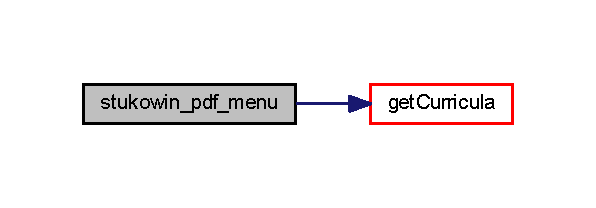
\includegraphics[width=286pt]{group___drupal2_p_d_f_ga3649714a54a489d8c0096116fd9cb367_cgraph}
\end{center}
\end{figure}


\hypertarget{group___drupal2_p_d_f_ga7fd34094c899b5a82949f401e30139a1}{\index{Drupal2\+P\+D\+F@{Drupal2\+P\+D\+F}!stukowin\+\_\+pdf\+\_\+menu\+\_\+submit@{stukowin\+\_\+pdf\+\_\+menu\+\_\+submit}}
\index{stukowin\+\_\+pdf\+\_\+menu\+\_\+submit@{stukowin\+\_\+pdf\+\_\+menu\+\_\+submit}!Drupal2\+P\+D\+F@{Drupal2\+P\+D\+F}}
\paragraph[{stukowin\+\_\+pdf\+\_\+menu\+\_\+submit}]{\setlength{\rightskip}{0pt plus 5cm}stukowin\+\_\+pdf\+\_\+menu\+\_\+submit (
\begin{DoxyParamCaption}
\item[{}]{\$form, }
\item[{\&}]{\$form\+\_\+state}
\end{DoxyParamCaption}
)}}\label{group___drupal2_p_d_f_ga7fd34094c899b5a82949f401e30139a1}


Submit handler for \hyperlink{group___drupal2_p_d_f_ga3649714a54a489d8c0096116fd9cb367}{stukowin\+\_\+pdf\+\_\+menu()} 

Creates an instance of \hyperlink{classoverview_p_d_f}{overview\+P\+D\+F} and starts the document generation. If successful, the full path of the generated document is displayed.


\begin{DoxyParams}[1]{Parameters}
array & {\em \$form} & Form structure as given by Drupal \\
\hline
array & {\em \$form\+\_\+state} & Form state as given by Drupal\\
\hline
\end{DoxyParams}
\begin{DoxyAuthor}{Author}
Jakob Strasser -\/ \href{mailto:jakob.strasser@telenet.be}{\tt jakob.\+strasser@telenet.\+be} 
\end{DoxyAuthor}
\begin{DoxyVersion}{Version}
1.\+0.\+0 2014-\/07-\/16 
\end{DoxyVersion}
\begin{DoxySince}{Since}
Commit \href{http://github.com/TheJake123/DrupalModul/commit/e6573f8d945918d261f42b421be6e5de94881a0b}{\tt e6573f8} on 2014-\/06-\/30
\end{DoxySince}
\begin{DoxySeeAlso}{See also}
\hyperlink{group___drupal2_p_d_f_ga3649714a54a489d8c0096116fd9cb367}{stukowin\+\_\+pdf\+\_\+menu()} 

\hyperlink{classoverview_p_d_f_a30ddd92aaf87bca0825c149bd3a7d43f}{overview\+P\+D\+F\+::create\+P\+D\+F()} 
\end{DoxySeeAlso}


Definition at line 224 of file stukowin.\+module.


\hypertarget{group___stukowin___module}{\subsection{Module Core}
\label{group___stukowin___module}\index{Module Core@{Module Core}}
}


Module that contains core functionality.  


\subsubsection*{Files}
\begin{DoxyCompactItemize}
\item 
file \hyperlink{content__manager_8inc_8php}{content\+\_\+manager.\+inc.\+php}
\begin{DoxyCompactList}\small\item\em Access to curricula data. \end{DoxyCompactList}\item 
file \hyperlink{stukowin_8install}{stukowin.\+install}
\begin{DoxyCompactList}\small\item\em Install script. \end{DoxyCompactList}\end{DoxyCompactItemize}
\subsubsection*{Data Structures}
\begin{DoxyCompactItemize}
\item 
class \hyperlink{classcontent__manager}{content\+\_\+manager}
\begin{DoxyCompactList}\small\item\em Access to drupal vocabularies and content nodes. \end{DoxyCompactList}\end{DoxyCompactItemize}
\subsubsection*{Functions}
\begin{DoxyCompactItemize}
\item 
\hyperlink{group___stukowin___module_ga67989d3a763f2efa2fc0b07460639558}{stukowin\+\_\+install} ()
\begin{DoxyCompactList}\small\item\em Implements hook\+\_\+install(). \end{DoxyCompactList}\item 
\hyperlink{group___stukowin___module_ga0dbd0252e3db9efdb3cfefbefecf3d2e}{\+\_\+stukowin\+\_\+installed\+\_\+taxonomy\+\_\+fields} ()
\begin{DoxyCompactList}\small\item\em Contains the array of additional vocabulary fields. \end{DoxyCompactList}\item 
\hyperlink{group___stukowin___module_gafd634a2fb5766e1053fa7df79ab11c79}{\+\_\+stukowin\+\_\+installed\+\_\+taxonomy\+\_\+instances} ()
\begin{DoxyCompactList}\small\item\em Contains the array of additional fields for vocabulary instances. \end{DoxyCompactList}\item 
\hyperlink{group___stukowin___module_ga5eda7b9b561e8a5ad87df0bb50cf80b0}{\+\_\+stukowin\+\_\+installed\+\_\+fields} ()
\begin{DoxyCompactList}\small\item\em Contains the array of additional fields for the stukowin content node type. \end{DoxyCompactList}\item 
\hyperlink{group___stukowin___module_ga473e908d001c086718d6675f19cb7ee7}{\+\_\+stukowin\+\_\+installed\+\_\+instances} ()
\begin{DoxyCompactList}\small\item\em Contains the array of additional fields for the stukowin content node type. \end{DoxyCompactList}\item 
\hyperlink{group___stukowin___module_gae7b4c9b6b19887d0ccc914b2886010ce}{\+\_\+stukowin\+\_\+relation\+\_\+types} ()
\begin{DoxyCompactList}\small\item\em Contains custom relation types for recommendations and requirements. \end{DoxyCompactList}\item 
\hyperlink{group___stukowin___module_gac59bc3fe951ab5625be92cfbff7e3dc4}{\+\_\+stukowin\+\_\+create\+\_\+relation\+\_\+types} ()
\begin{DoxyCompactList}\small\item\em Creates the relation type. \end{DoxyCompactList}\item 
\hyperlink{group___stukowin___module_gad831696eae7eb1a0e48c4e9621323bca}{stukowin\+\_\+uninstall} ()
\begin{DoxyCompactList}\small\item\em Implements hook\+\_\+uninstall(). \end{DoxyCompactList}\item 
\hyperlink{group___stukowin___module_ga55d453d5b6f8ae4e643308d8814e67a5}{stukowin\+\_\+admin} ()
\begin{DoxyCompactList}\small\item\em Menu callback for module settings (\char`\"{}admin/stukowin/settings\char`\"{}) \end{DoxyCompactList}\item 
\hyperlink{group___stukowin___module_ga59cfbad113b7aa2d10f0b204a5f7ba0d}{stukowin\+\_\+menu} ()
\begin{DoxyCompactList}\small\item\em Implements hook\+\_\+menu(). \end{DoxyCompactList}\end{DoxyCompactItemize}


\subsubsection{Detailed Description}
Module that contains core functionality. 

This module contains all files, classes and methods that provide the core functionality of the Drupal module. The members of this group ensure a working cooperation between all of the components and Drupal.

\begin{DoxyAuthor}{Authors}
Konstantinos Dafalias -\/ \href{mailto:kdafalias@gmail.com}{\tt kdafalias@gmail.\+com} 

Jakob Strasser -\/ \href{mailto:jakob.strasser@telenet.be}{\tt jakob.\+strasser@telenet.\+be} 

Werner Breuer -\/ \href{mailto:bluescreenwerner@gmail.com}{\tt bluescreenwerner@gmail.\+com} 

Markus Gutmayer -\/ \href{mailto:m.gutmayer@gmail.com}{\tt m.\+gutmayer@gmail.\+com} 
\end{DoxyAuthor}


\subsubsection{Function Documentation}
\hypertarget{group___stukowin___module_gac59bc3fe951ab5625be92cfbff7e3dc4}{\index{Module Core@{Module Core}!\+\_\+stukowin\+\_\+create\+\_\+relation\+\_\+types@{\+\_\+stukowin\+\_\+create\+\_\+relation\+\_\+types}}
\index{\+\_\+stukowin\+\_\+create\+\_\+relation\+\_\+types@{\+\_\+stukowin\+\_\+create\+\_\+relation\+\_\+types}!Module Core@{Module Core}}
\paragraph[{\+\_\+stukowin\+\_\+create\+\_\+relation\+\_\+types}]{\setlength{\rightskip}{0pt plus 5cm}\+\_\+stukowin\+\_\+create\+\_\+relation\+\_\+types (
\begin{DoxyParamCaption}
{}
\end{DoxyParamCaption}
)}}\label{group___stukowin___module_gac59bc3fe951ab5625be92cfbff7e3dc4}


Creates the relation type. 

This method creates the relation type for course recommendations and requirements

\begin{DoxyVersion}{Version}
1.\+0.\+0 2014-\/07-\/07 
\end{DoxyVersion}
\begin{DoxyAuthor}{Author}
Konstantinos Dafalias -\/ \href{mailto:kdafalias@gmail.com}{\tt kdafalias@gmail.\+com} 
\end{DoxyAuthor}
\begin{DoxySince}{Since}
Commit \href{http://github.com/TheJake123/DrupalModul/commit/d179abcc5e05743086cd67cf1ce30b08923a7183}{\tt d179abc} on 2014-\/06-\/28 
\end{DoxySince}


Definition at line 629 of file stukowin.\+install.



References \+\_\+stukowin\+\_\+relation\+\_\+types().



Referenced by stukowin\+\_\+install().



Here is the call graph for this function\+:
\nopagebreak
\begin{figure}[H]
\begin{center}
\leavevmode
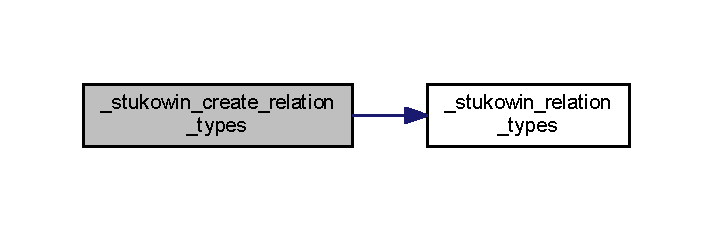
\includegraphics[width=342pt]{group___stukowin___module_gac59bc3fe951ab5625be92cfbff7e3dc4_cgraph}
\end{center}
\end{figure}




Here is the caller graph for this function\+:
\nopagebreak
\begin{figure}[H]
\begin{center}
\leavevmode
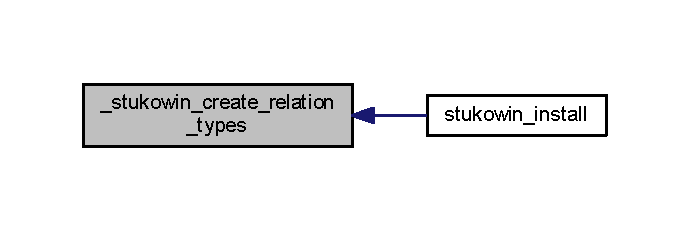
\includegraphics[width=331pt]{group___stukowin___module_gac59bc3fe951ab5625be92cfbff7e3dc4_icgraph}
\end{center}
\end{figure}


\hypertarget{group___stukowin___module_ga5eda7b9b561e8a5ad87df0bb50cf80b0}{\index{Module Core@{Module Core}!\+\_\+stukowin\+\_\+installed\+\_\+fields@{\+\_\+stukowin\+\_\+installed\+\_\+fields}}
\index{\+\_\+stukowin\+\_\+installed\+\_\+fields@{\+\_\+stukowin\+\_\+installed\+\_\+fields}!Module Core@{Module Core}}
\paragraph[{\+\_\+stukowin\+\_\+installed\+\_\+fields}]{\setlength{\rightskip}{0pt plus 5cm}\+\_\+stukowin\+\_\+installed\+\_\+fields (
\begin{DoxyParamCaption}
{}
\end{DoxyParamCaption}
)}}\label{group___stukowin___module_ga5eda7b9b561e8a5ad87df0bb50cf80b0}


Contains the array of additional fields for the stukowin content node type. 

Return a structured array defining the fields created by this content type. The additional fields are\+:
\begin{DoxyItemize}
\item ceusid
\item code
\item ects
\item wst
\item verantname
\item verantemail
\item changedate
\item lvtypname
\item lvtypshort
\item lvatype
\item typename
\item ziele
\item lehrinhalte
\item voraussetzungen
\item voraussetzung
\item empfehlung
\item term of the course as received from C\+E\+U\+S and saved in Drupal. \begin{DoxyReturn}{Returns}
A structured array for Drupal field generation
\end{DoxyReturn}
\begin{DoxyVersion}{Version}
1.\+0.\+0 2014-\/07-\/07 
\end{DoxyVersion}
\begin{DoxyAuthor}{Author}
Konstantinos Dafalias -\/ \href{mailto:kdafalias@gmail.com}{\tt kdafalias@gmail.\+com} 
\end{DoxyAuthor}
\begin{DoxySince}{Since}
Commit \href{http://github.com/TheJake123/DrupalModul/commit/d179abcc5e05743086cd67cf1ce30b08923a7183}{\tt d179abc} on 2014-\/06-\/28 
\end{DoxySince}

\end{DoxyItemize}

Definition at line 209 of file stukowin.\+install.



Referenced by content\+\_\+manager\+::get\+\_\+return\+\_\+node(), stukowin\+\_\+install(), stukowin\+\_\+uninstall(), and content\+\_\+manager\+::taxonomy\+\_\+get\+\_\+nested\+\_\+tree().



Here is the caller graph for this function\+:
\nopagebreak
\begin{figure}[H]
\begin{center}
\leavevmode
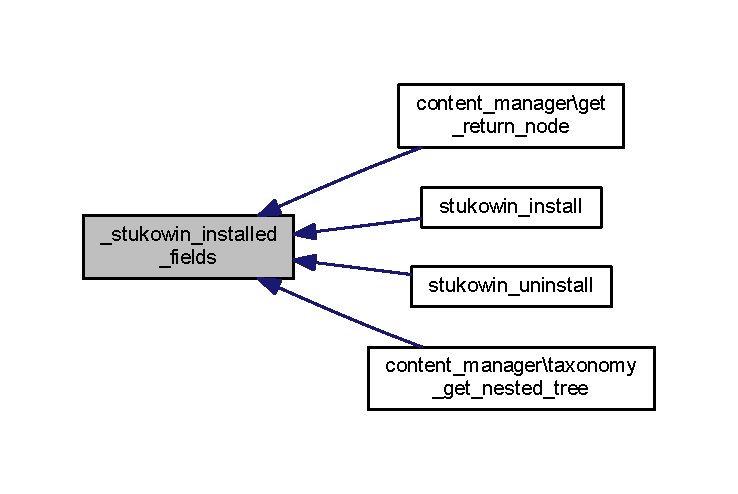
\includegraphics[width=350pt]{group___stukowin___module_ga5eda7b9b561e8a5ad87df0bb50cf80b0_icgraph}
\end{center}
\end{figure}


\hypertarget{group___stukowin___module_ga473e908d001c086718d6675f19cb7ee7}{\index{Module Core@{Module Core}!\+\_\+stukowin\+\_\+installed\+\_\+instances@{\+\_\+stukowin\+\_\+installed\+\_\+instances}}
\index{\+\_\+stukowin\+\_\+installed\+\_\+instances@{\+\_\+stukowin\+\_\+installed\+\_\+instances}!Module Core@{Module Core}}
\paragraph[{\+\_\+stukowin\+\_\+installed\+\_\+instances}]{\setlength{\rightskip}{0pt plus 5cm}\+\_\+stukowin\+\_\+installed\+\_\+instances (
\begin{DoxyParamCaption}
{}
\end{DoxyParamCaption}
)}}\label{group___stukowin___module_ga473e908d001c086718d6675f19cb7ee7}


Contains the array of additional fields for the stukowin content node type. 

Return a structured array defining and describing in greater detail the fields created by this content type. The additional fields are\+:
\begin{DoxyItemize}
\item ceusid
\item code
\item ects
\item wst
\item verantname
\item verantemail
\item changedate
\item lvtypname
\item lvtypshort
\item lvatype
\item typename
\item ziele
\item lehrinhalte
\item voraussetzungen
\item voraussetzung
\item empfehlung
\item term of the course as received from C\+E\+U\+S and saved in Drupal. \begin{DoxyReturn}{Returns}
A structured array for Drupal field generation
\end{DoxyReturn}
\begin{DoxyVersion}{Version}
1.\+0.\+0 2014-\/07-\/07 
\end{DoxyVersion}
\begin{DoxyAuthor}{Author}
Konstantinos Dafalias -\/ \href{mailto:kdafalias@gmail.com}{\tt kdafalias@gmail.\+com} 
\end{DoxyAuthor}
\begin{DoxyAuthor}{Authors}
Fabian Puehringer -\/ \href{mailto:f.puehringer@24speed.at}{\tt f.\+puehringer@24speed.\+at} 
\end{DoxyAuthor}
\begin{DoxySince}{Since}
Commit \href{http://github.com/TheJake123/DrupalModul/commit/d179abcc5e05743086cd67cf1ce30b08923a7183}{\tt d179abc} on 2014-\/06-\/28 
\end{DoxySince}

\end{DoxyItemize}

Definition at line 334 of file stukowin.\+install.



Referenced by stukowin\+\_\+install().



Here is the caller graph for this function\+:
\nopagebreak
\begin{figure}[H]
\begin{center}
\leavevmode
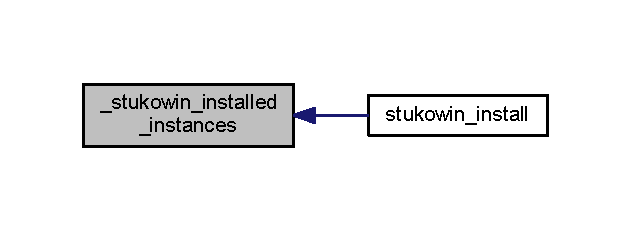
\includegraphics[width=303pt]{group___stukowin___module_ga473e908d001c086718d6675f19cb7ee7_icgraph}
\end{center}
\end{figure}


\hypertarget{group___stukowin___module_ga0dbd0252e3db9efdb3cfefbefecf3d2e}{\index{Module Core@{Module Core}!\+\_\+stukowin\+\_\+installed\+\_\+taxonomy\+\_\+fields@{\+\_\+stukowin\+\_\+installed\+\_\+taxonomy\+\_\+fields}}
\index{\+\_\+stukowin\+\_\+installed\+\_\+taxonomy\+\_\+fields@{\+\_\+stukowin\+\_\+installed\+\_\+taxonomy\+\_\+fields}!Module Core@{Module Core}}
\paragraph[{\+\_\+stukowin\+\_\+installed\+\_\+taxonomy\+\_\+fields}]{\setlength{\rightskip}{0pt plus 5cm}\+\_\+stukowin\+\_\+installed\+\_\+taxonomy\+\_\+fields (
\begin{DoxyParamCaption}
{}
\end{DoxyParamCaption}
)}}\label{group___stukowin___module_ga0dbd0252e3db9efdb3cfefbefecf3d2e}


Contains the array of additional vocabulary fields. 

Returns a structured array defining the custom fields for vocabularies. The additional fields are\+:
\begin{DoxyItemize}
\item faculty
\item version
\item type of curriculum as received from C\+E\+U\+S.
\end{DoxyItemize}

\begin{DoxyReturn}{Returns}
A structured array for Drupal field generation
\end{DoxyReturn}
\begin{DoxyVersion}{Version}
1.\+0.\+0 2014-\/07-\/07 
\end{DoxyVersion}
\begin{DoxyAuthor}{Author}
Konstantinos Dafalias -\/ \href{mailto:kdafalias@gmail.com}{\tt kdafalias@gmail.\+com} 
\end{DoxyAuthor}
\begin{DoxySince}{Since}
Commit \href{http://github.com/TheJake123/DrupalModul/commit/d179abcc5e05743086cd67cf1ce30b08923a7183}{\tt d179abc} on 2014-\/06-\/28
\end{DoxySince}
\begin{DoxySeeAlso}{See also}
\hyperlink{group___stukowin___module_gafd634a2fb5766e1053fa7df79ab11c79}{\+\_\+stukowin\+\_\+installed\+\_\+taxonomy\+\_\+instances()} 
\end{DoxySeeAlso}


Definition at line 103 of file stukowin.\+install.



Referenced by stukowin\+\_\+install(), and stukowin\+\_\+uninstall().



Here is the caller graph for this function\+:
\nopagebreak
\begin{figure}[H]
\begin{center}
\leavevmode
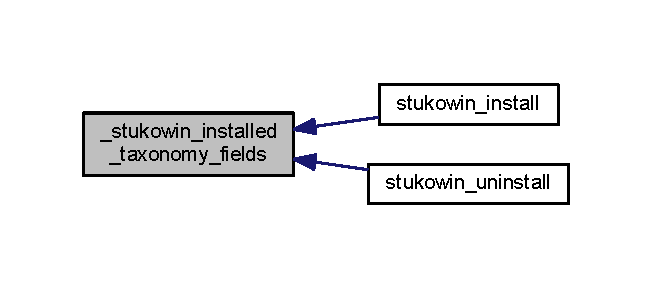
\includegraphics[width=313pt]{group___stukowin___module_ga0dbd0252e3db9efdb3cfefbefecf3d2e_icgraph}
\end{center}
\end{figure}


\hypertarget{group___stukowin___module_gafd634a2fb5766e1053fa7df79ab11c79}{\index{Module Core@{Module Core}!\+\_\+stukowin\+\_\+installed\+\_\+taxonomy\+\_\+instances@{\+\_\+stukowin\+\_\+installed\+\_\+taxonomy\+\_\+instances}}
\index{\+\_\+stukowin\+\_\+installed\+\_\+taxonomy\+\_\+instances@{\+\_\+stukowin\+\_\+installed\+\_\+taxonomy\+\_\+instances}!Module Core@{Module Core}}
\paragraph[{\+\_\+stukowin\+\_\+installed\+\_\+taxonomy\+\_\+instances}]{\setlength{\rightskip}{0pt plus 5cm}\+\_\+stukowin\+\_\+installed\+\_\+taxonomy\+\_\+instances (
\begin{DoxyParamCaption}
{}
\end{DoxyParamCaption}
)}}\label{group___stukowin___module_gafd634a2fb5766e1053fa7df79ab11c79}


Contains the array of additional fields for vocabulary instances. 

Returns a structured array defining and describing in greater detail the custom fields for vocabularies. The additional fields are\+:
\begin{DoxyItemize}
\item faculty
\item version
\item type of curriculum as received from C\+E\+U\+S.
\end{DoxyItemize}

\begin{DoxyReturn}{Returns}
A structured array for drupal field instance generation
\end{DoxyReturn}
\begin{DoxyVersion}{Version}
1.\+0.\+0 2014-\/07-\/07 
\end{DoxyVersion}
\begin{DoxyAuthor}{Author}
Konstantinos Dafalias -\/ \href{mailto:kdafalias@gmail.com}{\tt kdafalias@gmail.\+com} 
\end{DoxyAuthor}
\begin{DoxySince}{Since}
Commit \href{http://github.com/TheJake123/DrupalModul/commit/d179abcc5e05743086cd67cf1ce30b08923a7183}{\tt d179abc} on 2014-\/06-\/28
\end{DoxySince}
\begin{DoxySeeAlso}{See also}
\hyperlink{group___stukowin___module_ga0dbd0252e3db9efdb3cfefbefecf3d2e}{\+\_\+stukowin\+\_\+installed\+\_\+taxonomy\+\_\+fields()} 
\end{DoxySeeAlso}


Definition at line 147 of file stukowin.\+install.



Referenced by stukowin\+\_\+install().



Here is the caller graph for this function\+:
\nopagebreak
\begin{figure}[H]
\begin{center}
\leavevmode

\includegraphics[width=314pt]{group___stukowin___module_gafd634a2fb5766e1053fa7df79ab11c79_icgraph}
\end{center}
\end{figure}


\hypertarget{group___stukowin___module_gae7b4c9b6b19887d0ccc914b2886010ce}{\index{Module Core@{Module Core}!\+\_\+stukowin\+\_\+relation\+\_\+types@{\+\_\+stukowin\+\_\+relation\+\_\+types}}
\index{\+\_\+stukowin\+\_\+relation\+\_\+types@{\+\_\+stukowin\+\_\+relation\+\_\+types}!Module Core@{Module Core}}
\paragraph[{\+\_\+stukowin\+\_\+relation\+\_\+types}]{\setlength{\rightskip}{0pt plus 5cm}\+\_\+stukowin\+\_\+relation\+\_\+types (
\begin{DoxyParamCaption}
{}
\end{DoxyParamCaption}
)}}\label{group___stukowin___module_gae7b4c9b6b19887d0ccc914b2886010ce}


Contains custom relation types for recommendations and requirements. 

\begin{DoxyReturn}{Returns}
An array containing the description for recommended and required prerequisite relations.
\end{DoxyReturn}
\begin{DoxyVersion}{Version}
1.\+0.\+0 2014-\/07-\/07 
\end{DoxyVersion}
\begin{DoxyAuthor}{Author}
Konstantinos Dafalias -\/ \href{mailto:kdafalias@gmail.com}{\tt kdafalias@gmail.\+com} 
\end{DoxyAuthor}
\begin{DoxySince}{Since}
Commit \href{http://github.com/TheJake123/DrupalModul/commit/d179abcc5e05743086cd67cf1ce30b08923a7183}{\tt d179abc} on 2014-\/06-\/28 
\end{DoxySince}


Definition at line 607 of file stukowin.\+install.



Referenced by \+\_\+stukowin\+\_\+create\+\_\+relation\+\_\+types(), and stukowin\+\_\+uninstall().



Here is the caller graph for this function\+:
\nopagebreak
\begin{figure}[H]
\begin{center}
\leavevmode
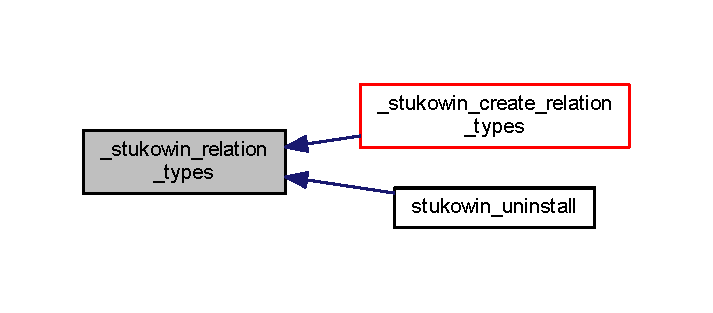
\includegraphics[width=342pt]{group___stukowin___module_gae7b4c9b6b19887d0ccc914b2886010ce_icgraph}
\end{center}
\end{figure}


\hypertarget{group___stukowin___module_ga55d453d5b6f8ae4e643308d8814e67a5}{\index{Module Core@{Module Core}!stukowin\+\_\+admin@{stukowin\+\_\+admin}}
\index{stukowin\+\_\+admin@{stukowin\+\_\+admin}!Module Core@{Module Core}}
\paragraph[{stukowin\+\_\+admin}]{\setlength{\rightskip}{0pt plus 5cm}stukowin\+\_\+admin (
\begin{DoxyParamCaption}
{}
\end{DoxyParamCaption}
)}}\label{group___stukowin___module_ga55d453d5b6f8ae4e643308d8814e67a5}


Menu callback for module settings (\char`\"{}admin/stukowin/settings\char`\"{}) 

Form for administration of the module settings This form has the following input fields\+:
\begin{DoxyItemize}
\item C\+E\+U\+S A\+P\+I Settings
\begin{DoxyItemize}
\item U\+R\+L to C\+E\+U\+S A\+P\+I
\item Username for C\+E\+U\+S A\+P\+I
\item Password for C\+E\+U\+S A\+P\+I
\item Last Update from C\+E\+U\+S A\+P\+I
\end{DoxyItemize}
\item P\+D\+F Settings
\begin{DoxyItemize}
\item P\+D\+F Path
\item P\+D\+F generic name
\end{DoxyItemize}
\end{DoxyItemize}

\begin{DoxyReturn}{Returns}
An array containing the form structure
\end{DoxyReturn}
\begin{DoxyAuthor}{Authors}
Konstantinos Dafalias -\/ \href{mailto:kdafalias@gmail.com}{\tt kdafalias@gmail.\+com} 

Jakob Strasser -\/ \href{mailto:jakob.strasser@telenet.be}{\tt jakob.\+strasser@telenet.\+be} 
\end{DoxyAuthor}
\begin{DoxyVersion}{Version}
1.\+0.\+0 2014-\/07-\/16 
\end{DoxyVersion}
\begin{DoxySince}{Since}
Commit \href{http://github.com/TheJake123/DrupalModul/commit/d179abcc5e05743086cd67cf1ce30b08923a7183}{\tt d179abc} on 2014-\/06-\/28 
\end{DoxySince}


Definition at line 105 of file stukowin.\+module.

\hypertarget{group___stukowin___module_ga67989d3a763f2efa2fc0b07460639558}{\index{Module Core@{Module Core}!stukowin\+\_\+install@{stukowin\+\_\+install}}
\index{stukowin\+\_\+install@{stukowin\+\_\+install}!Module Core@{Module Core}}
\paragraph[{stukowin\+\_\+install}]{\setlength{\rightskip}{0pt plus 5cm}stukowin\+\_\+install (
\begin{DoxyParamCaption}
{}
\end{DoxyParamCaption}
)}}\label{group___stukowin___module_ga67989d3a763f2efa2fc0b07460639558}


Implements hook\+\_\+install(). 

Sets up drupal for use with the stukowin module.
\begin{DoxyItemize}
\item Creates the content type for L\+V\+A nodes.
\item Creates relation types for requirements and recommendations.
\item Adds 3 fields to taxonomy nodes for {\ttfamily faculty}, {\ttfamily version} and {\ttfamily type} of curriculum
\end{DoxyItemize}

\begin{DoxyAuthor}{Authors}
Konstantinos Dafalias -\/ \href{mailto:kdafalias@gmail.com}{\tt kdafalias@gmail.\+com} 

Jakob Strasser -\/ \href{mailto:jakob.strasser@telenet.be}{\tt jakob.\+strasser@telenet.\+be} 
\end{DoxyAuthor}
\begin{DoxyVersion}{Version}
1.\+0.\+0 2014-\/07-\/07 
\end{DoxyVersion}
\begin{DoxySince}{Since}
Commit \href{http://github.com/TheJake123/DrupalModul/commit/d179abcc5e05743086cd67cf1ce30b08923a7183}{\tt d179abc} on 2014-\/06-\/28 
\end{DoxySince}


Definition at line 30 of file stukowin.\+install.



References \+\_\+stukowin\+\_\+create\+\_\+relation\+\_\+types(), \+\_\+stukowin\+\_\+installed\+\_\+fields(), \+\_\+stukowin\+\_\+installed\+\_\+instances(), \+\_\+stukowin\+\_\+installed\+\_\+taxonomy\+\_\+fields(), and \+\_\+stukowin\+\_\+installed\+\_\+taxonomy\+\_\+instances().



Here is the call graph for this function\+:
\nopagebreak
\begin{figure}[H]
\begin{center}
\leavevmode
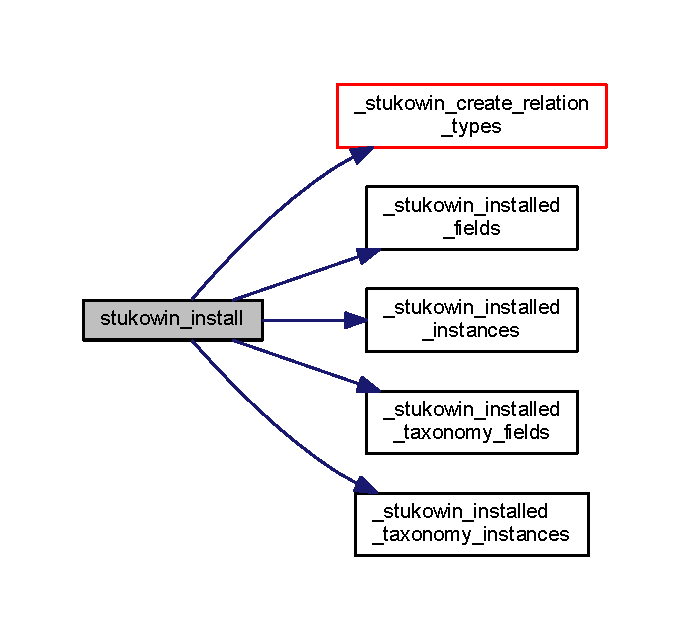
\includegraphics[width=331pt]{group___stukowin___module_ga67989d3a763f2efa2fc0b07460639558_cgraph}
\end{center}
\end{figure}


\hypertarget{group___stukowin___module_ga59cfbad113b7aa2d10f0b204a5f7ba0d}{\index{Module Core@{Module Core}!stukowin\+\_\+menu@{stukowin\+\_\+menu}}
\index{stukowin\+\_\+menu@{stukowin\+\_\+menu}!Module Core@{Module Core}}
\paragraph[{stukowin\+\_\+menu}]{\setlength{\rightskip}{0pt plus 5cm}stukowin\+\_\+menu (
\begin{DoxyParamCaption}
{}
\end{DoxyParamCaption}
)}}\label{group___stukowin___module_ga59cfbad113b7aa2d10f0b204a5f7ba0d}


Implements hook\+\_\+menu(). 

Registers all menu links with Drupal. The following links are registered\+:
\begin{DoxyItemize}
\item C\+E\+U\+S A\+P\+I Settings @ 'admin/stukowin/settings'
\item C\+E\+U\+S Data import @ 'admin/settings/stukowin/import'
\item P\+D\+F Generation @ 'admin/settings/stukowin/pdf'
\item I\+T\+S\+V/\+Specialisation Taxonomy Creation @ 'admin/settings/stukowin/taxonomy'
\item Curriculum J\+S\+O\+N Service @ 'stukowin/crclm'
\item Curricula List J\+S\+O\+N Service @ 'stukowin/crclmlst'
\item Course Detail J\+S\+O\+N Service @ 'stukowin/lva'
\end{DoxyItemize}

\begin{DoxyAuthor}{Authors}
Konstantinos Dafalias -\/ \href{mailto:kdafalias@gmail.com}{\tt kdafalias@gmail.\+com} 

Jakob Strasser -\/ \href{mailto:jakob.strasser@telenet.be}{\tt jakob.\+strasser@telenet.\+be} 

Werner Breuer -\/ \href{mailto:bluescreenwerner@gmail.com}{\tt bluescreenwerner@gmail.\+com} 
\end{DoxyAuthor}
\begin{DoxyVersion}{Version}
1.\+0.\+0 2014-\/07-\/16 
\end{DoxyVersion}
\begin{DoxySince}{Since}
Commit \href{http://github.com/TheJake123/DrupalModul/commit/d179abcc5e05743086cd67cf1ce30b08923a7183}{\tt d179abc} on 2014-\/06-\/28
\end{DoxySince}
\begin{DoxySeeAlso}{See also}
\hyperlink{group___drupal2_p_d_f_ga3649714a54a489d8c0096116fd9cb367}{stukowin\+\_\+pdf\+\_\+menu()} 

\hyperlink{group___drupal2_i_t_s_v_gab706d935ca9d9998c5e25a9ad6486d6a}{stukowin\+\_\+taxonomy\+\_\+menu()} 

\hyperlink{group___c_e_u_s2_drupal_ga481789ce9904fc10aefb8eaf7534133b}{stukowin\+\_\+pre\+\_\+retreive()} 

\hyperlink{group___stukowin___module_ga55d453d5b6f8ae4e643308d8814e67a5}{stukowin\+\_\+admin()} 

\hyperlink{group___drupal2_a_g_g_ga7522e206f1a87971b916a7a0be0098c6}{stukowin\+\_\+get\+\_\+lva()} 

\hyperlink{group___drupal2_a_g_g_gaf137f10bef98707dacaf33d6581773d0}{stukowin\+\_\+get\+\_\+crclm\+\_\+taxonomy()} 

\hyperlink{group___drupal2_a_g_g_gad0cb4d7faa68097f5b7df8311e36b22e}{stukowin\+\_\+get\+\_\+crclm\+\_\+list()} 
\end{DoxySeeAlso}


Definition at line 507 of file stukowin.\+module.

\hypertarget{group___stukowin___module_gad831696eae7eb1a0e48c4e9621323bca}{\index{Module Core@{Module Core}!stukowin\+\_\+uninstall@{stukowin\+\_\+uninstall}}
\index{stukowin\+\_\+uninstall@{stukowin\+\_\+uninstall}!Module Core@{Module Core}}
\paragraph[{stukowin\+\_\+uninstall}]{\setlength{\rightskip}{0pt plus 5cm}stukowin\+\_\+uninstall (
\begin{DoxyParamCaption}
{}
\end{DoxyParamCaption}
)}}\label{group___stukowin___module_gad831696eae7eb1a0e48c4e9621323bca}


Implements hook\+\_\+uninstall(). 


\begin{DoxyItemize}
\item Deletes all content nodes
\item Deletes all C\+E\+U\+S taxonomies
\item Deletes the content type for L\+V\+A nodes
\end{DoxyItemize}

\begin{DoxyVersion}{Version}
1.\+0.\+0 2014-\/07-\/09 
\end{DoxyVersion}
\begin{DoxyAuthor}{Author}
Konstantinos Dafalias -\/ \href{mailto:kdafalias@gmail.com}{\tt kdafalias@gmail.\+com} 

Jakob Strasser -\/ \href{mailto:jakob.strasser@telenet.be}{\tt jakob.\+strasser@telenet.\+be} 

Werner Breuer -\/ \href{mailto:bluescreenwerner@gmail.com}{\tt bluescreenwerner@gmail.\+com}
\end{DoxyAuthor}
\begin{DoxySince}{Since}
Commit \href{http://github.com/TheJake123/DrupalModul/commit/2506486a98691dbd0031666d5f932784bd3eede1}{\tt 2506486} on 2014-\/07-\/09 
\end{DoxySince}


Definition at line 662 of file stukowin.\+install.



References \+\_\+stukowin\+\_\+installed\+\_\+fields(), \+\_\+stukowin\+\_\+installed\+\_\+taxonomy\+\_\+fields(), and \+\_\+stukowin\+\_\+relation\+\_\+types().



Here is the call graph for this function\+:
\nopagebreak
\begin{figure}[H]
\begin{center}
\leavevmode
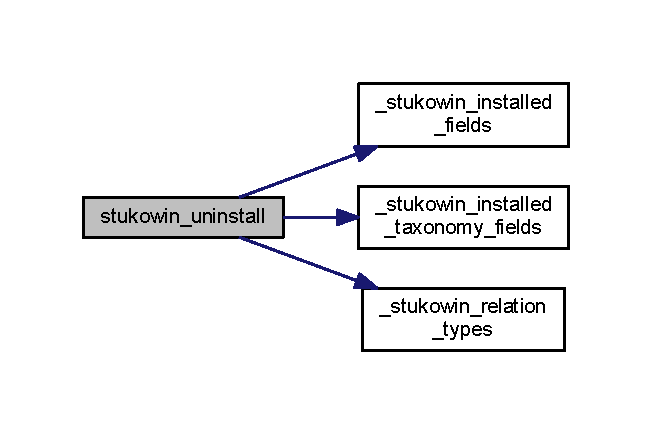
\includegraphics[width=313pt]{group___stukowin___module_gad831696eae7eb1a0e48c4e9621323bca_cgraph}
\end{center}
\end{figure}



\hypertarget{group___drupal2_i_t_s_v}{\subsection{Drupal2\+I\+T\+S\+V}
\label{group___drupal2_i_t_s_v}\index{Drupal2\+I\+T\+S\+V@{Drupal2\+I\+T\+S\+V}}
}


Module to create new Drupal I\+T\+S\+V/specialisation vocabularies.  


\subsubsection*{Functions}
\begin{DoxyCompactItemize}
\item 
\hyperlink{group___drupal2_i_t_s_v_gab706d935ca9d9998c5e25a9ad6486d6a}{stukowin\+\_\+taxonomy\+\_\+menu} (\$form, \&\$form\+\_\+state)
\begin{DoxyCompactList}\small\item\em Menu callback for creating a new I\+T\+S\+V or specialisation vocabulary. \end{DoxyCompactList}\item 
\hyperlink{group___drupal2_i_t_s_v_ga5fb85a53362f6fef40035a6c350c11ea}{stukowin\+\_\+taxonomy\+\_\+menu\+\_\+submit} (\$form, \&\$form\+\_\+state)
\begin{DoxyCompactList}\small\item\em Submit handler for \hyperlink{group___drupal2_i_t_s_v_gab706d935ca9d9998c5e25a9ad6486d6a}{stukowin\+\_\+taxonomy\+\_\+menu()} \end{DoxyCompactList}\end{DoxyCompactItemize}


\subsubsection{Detailed Description}
Module to create new Drupal I\+T\+S\+V/specialisation vocabularies. 

This module contains all files, classes and methods that provide the functionality for supporting the administrator when creating new Drupal vocabularies that represent either an I\+T\+S\+V (\char`\"{}\+Idealtypischer Studienverlauf\char`\"{}) or a specialisation (mainly for Master curricula). 



As C\+E\+U\+S does not provide any information about fields of specialisation during the master studies and ideal courses of studies, henceforth called I\+T\+S\+V due to its German name, it was a project requirement that new curricula can be created by the administrator for such purposes.

A freely available Drupal module called Taxonomy Manager (\href{https://www.drupal.org/project/taxonomy_manager}{\tt https\+://www.\+drupal.\+org/project/taxonomy\+\_\+manager}) gives the administrator the ability to copy vocabulary terms from one vocabulary to another, which is most of the work. Unfortunately, this process cannot be simplified any further. Nevertheless, we tried to at least automate the task of creating a new vocabulary, copying all of the information over from the source curriculum and creating top-\/level terms (such as \char`\"{}1. Semester\char`\"{} etc.), tasks which will be performed every time a new I\+T\+S\+V or specialisation has to be created.

This component handles exactly that. It inserts a new menu item (at admin/settings/stukowin/taxonomy) where the administrator can select a source curriculum to base the new one on, select whether to create an I\+T\+S\+V or specialisation vocabulary, enter a name and choose how many top-\/level terms should be inserted. Once the administrator has filled out the form, the new vocabulary is automatically created and the browser is redirected to the Taxonomy Manager's \char`\"{}\+Dual View\char`\"{}, where the administrator can begin copying courses into the new vocabulary.

\begin{DoxyRemark}{Remarks}
This component does not have its own file as it does not contain a lot of code. All of its functionality is in the \hyperlink{stukowin_8module}{stukowin.\+module} file.
\end{DoxyRemark}
\begin{DoxyAuthor}{Author}
Jakob Strasser -\/ \href{mailto:jakob.strasser@telenet.be}{\tt jakob.\+strasser@telenet.\+be} 
\end{DoxyAuthor}
\begin{DoxyAuthor}{Authors}
Werner Breuer -\/ \href{mailto:bluescreenwerner@gmail.com}{\tt bluescreenwerner@gmail.\+com} 

Markus Gutmayer -\/ \href{mailto:m.gutmayer@gmail.com}{\tt m.\+gutmayer@gmail.\+com} 
\end{DoxyAuthor}


\subsubsection{Function Documentation}
\hypertarget{group___drupal2_i_t_s_v_gab706d935ca9d9998c5e25a9ad6486d6a}{\index{Drupal2\+I\+T\+S\+V@{Drupal2\+I\+T\+S\+V}!stukowin\+\_\+taxonomy\+\_\+menu@{stukowin\+\_\+taxonomy\+\_\+menu}}
\index{stukowin\+\_\+taxonomy\+\_\+menu@{stukowin\+\_\+taxonomy\+\_\+menu}!Drupal2\+I\+T\+S\+V@{Drupal2\+I\+T\+S\+V}}
\paragraph[{stukowin\+\_\+taxonomy\+\_\+menu}]{\setlength{\rightskip}{0pt plus 5cm}stukowin\+\_\+taxonomy\+\_\+menu (
\begin{DoxyParamCaption}
\item[{}]{\$form, }
\item[{\&}]{\$form\+\_\+state}
\end{DoxyParamCaption}
)}}\label{group___drupal2_i_t_s_v_gab706d935ca9d9998c5e25a9ad6486d6a}


Menu callback for creating a new I\+T\+S\+V or specialisation vocabulary. 

Allows the user to
\begin{DoxyItemize}
\item Select a source vocabulary
\item Choose which type of vocabulary to create (I\+T\+S\+V or specialisation)
\item Set a name for the new vocabulary
\item Choose how many structural terms (e.\+g. \char`\"{}1. Semester\char`\"{}, \char`\"{}2. Semester\char`\"{}) to automatically insert
\end{DoxyItemize}


\begin{DoxyParams}[1]{Parameters}
array & {\em \$form} & Form structure as given by Drupal \\
\hline
array & {\em \$form\+\_\+state} & Form state as given by Drupal \\
\hline
\end{DoxyParams}
\begin{DoxyReturn}{Returns}
The filled out form structure
\end{DoxyReturn}
\begin{DoxyAuthor}{Author}
Jakob Strasser -\/ \href{mailto:jakob.strasser@telenet.be}{\tt jakob.\+strasser@telenet.\+be} 
\end{DoxyAuthor}
\begin{DoxyVersion}{Version}
1.\+0.\+0 2014-\/07-\/16 
\end{DoxyVersion}
\begin{DoxySince}{Since}
Commit \href{http://github.com/TheJake123/DrupalModul/commit/d179abcc5e05743086cd67cf1ce30b08923a7183}{\tt d179abc} on 2014-\/06-\/28
\end{DoxySince}
\begin{DoxySeeAlso}{See also}
\hyperlink{group___drupal2_i_t_s_v_ga5fb85a53362f6fef40035a6c350c11ea}{stukowin\+\_\+taxonomy\+\_\+menu\+\_\+submit()} 
\end{DoxySeeAlso}


Definition at line 388 of file stukowin.\+module.



References get\+Curricula().



Here is the call graph for this function\+:
\nopagebreak
\begin{figure}[H]
\begin{center}
\leavevmode
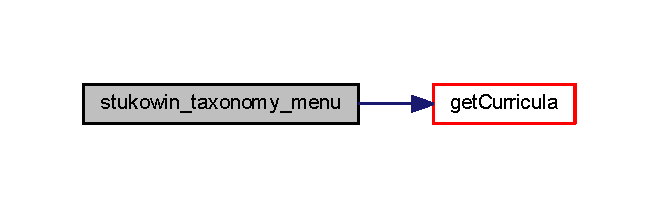
\includegraphics[width=316pt]{group___drupal2_i_t_s_v_gab706d935ca9d9998c5e25a9ad6486d6a_cgraph}
\end{center}
\end{figure}


\hypertarget{group___drupal2_i_t_s_v_ga5fb85a53362f6fef40035a6c350c11ea}{\index{Drupal2\+I\+T\+S\+V@{Drupal2\+I\+T\+S\+V}!stukowin\+\_\+taxonomy\+\_\+menu\+\_\+submit@{stukowin\+\_\+taxonomy\+\_\+menu\+\_\+submit}}
\index{stukowin\+\_\+taxonomy\+\_\+menu\+\_\+submit@{stukowin\+\_\+taxonomy\+\_\+menu\+\_\+submit}!Drupal2\+I\+T\+S\+V@{Drupal2\+I\+T\+S\+V}}
\paragraph[{stukowin\+\_\+taxonomy\+\_\+menu\+\_\+submit}]{\setlength{\rightskip}{0pt plus 5cm}stukowin\+\_\+taxonomy\+\_\+menu\+\_\+submit (
\begin{DoxyParamCaption}
\item[{}]{\$form, }
\item[{\&}]{\$form\+\_\+state}
\end{DoxyParamCaption}
)}}\label{group___drupal2_i_t_s_v_ga5fb85a53362f6fef40035a6c350c11ea}


Submit handler for \hyperlink{group___drupal2_i_t_s_v_gab706d935ca9d9998c5e25a9ad6486d6a}{stukowin\+\_\+taxonomy\+\_\+menu()} 

Creates a new I\+T\+S\+V or specialisation vocabulary and redirects the user to the taxonomy manager's dual view.


\begin{DoxyParams}[1]{Parameters}
array & {\em \$form} & Form structure as given by Drupal \\
\hline
array & {\em \$form\+\_\+state} & Form state as given by Drupal\\
\hline
\end{DoxyParams}
\begin{DoxyAuthor}{Author}
Jakob Strasser -\/ \href{mailto:jakob.strasser@telenet.be}{\tt jakob.\+strasser@telenet.\+be} 
\end{DoxyAuthor}
\begin{DoxyVersion}{Version}
1.\+0.\+0 2014-\/07-\/16 
\end{DoxyVersion}
\begin{DoxySince}{Since}
Commit \href{http://github.com/TheJake123/DrupalModul/commit/190577568295b7682dc74a79c4fd478e9e33c639}{\tt 1905775} on 2014-\/07-\/02
\end{DoxySince}
\begin{DoxySeeAlso}{See also}
\hyperlink{group___drupal2_i_t_s_v_gab706d935ca9d9998c5e25a9ad6486d6a}{stukowin\+\_\+taxonomy\+\_\+menu()} 
\end{DoxySeeAlso}


Definition at line 455 of file stukowin.\+module.


\section{Data Structure Documentation}
\hypertarget{classceus__importer}{\subsection{ceus\+\_\+importer Class Reference}
\label{classceus__importer}\index{ceus\+\_\+importer@{ceus\+\_\+importer}}
}


Imports data from C\+E\+U\+S and stores it in the Drupal database.  




Collaboration diagram for ceus\+\_\+importer\+:
\nopagebreak
\begin{figure}[H]
\begin{center}
\leavevmode
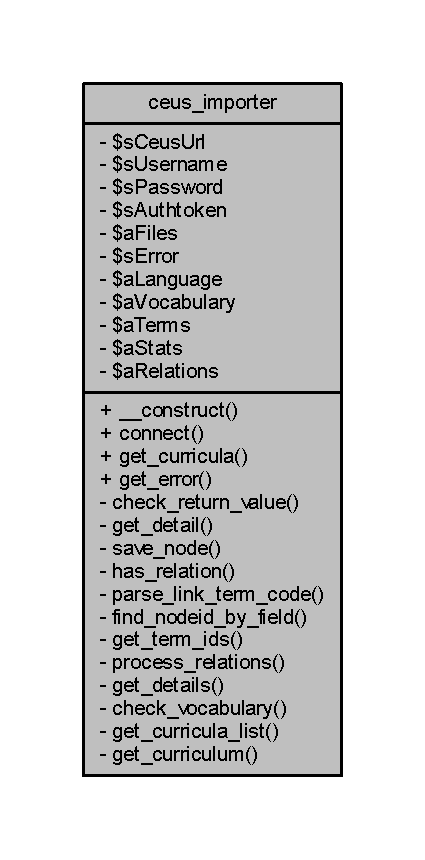
\includegraphics[width=204pt]{classceus__importer__coll__graph}
\end{center}
\end{figure}
\subsubsection*{Public Member Functions}
\begin{DoxyCompactItemize}
\item 
\hyperlink{classceus__importer_a095c5d389db211932136b53f25f39685}{\+\_\+\+\_\+construct} ()
\begin{DoxyCompactList}\small\item\em Constructor. \end{DoxyCompactList}\item 
\hyperlink{classceus__importer_a78572828d11dcdf2a498497d9001d557}{connect} ()
\begin{DoxyCompactList}\small\item\em Connect to C\+E\+U\+S and receive Authtoken. \end{DoxyCompactList}\item 
\hyperlink{classceus__importer_abd2f9a9afc073169b2badcb571cc983c}{get\+\_\+curricula} ()
\begin{DoxyCompactList}\small\item\em Main method\+: Imports curriculum data from C\+E\+U\+S. \end{DoxyCompactList}\item 
\hyperlink{classceus__importer_a1c0091515372f72e1a87683ca57c74eb}{get\+\_\+error} ()
\begin{DoxyCompactList}\small\item\em Returns last error message. \end{DoxyCompactList}\end{DoxyCompactItemize}
\subsubsection*{Private Member Functions}
\begin{DoxyCompactItemize}
\item 
\hyperlink{classceus__importer_a9147e757eb1c4c80e2720b160b86c239}{check\+\_\+return\+\_\+value} (\$s\+Return)
\begin{DoxyCompactList}\small\item\em Checks the J\+S\+O\+N returned by the C\+E\+U\+S A\+P\+I. \end{DoxyCompactList}\item 
\hyperlink{classceus__importer_a1b7d86575274b687d8e2fa9b29d7f7ba}{get\+\_\+detail} (\$i\+I\+D)
\begin{DoxyCompactList}\small\item\em Fetches a single course from C\+E\+U\+S. \end{DoxyCompactList}\item 
\hyperlink{classceus__importer_ae963f27a37b0a77da7c6f6c936625d3c}{save\+\_\+node} (\$a\+Detail, \$tid)
\begin{DoxyCompactList}\small\item\em Saves a course as a Drupal content node. \end{DoxyCompactList}\item 
\hyperlink{classceus__importer_a689c3df400e042323dcfc8a70bb86c0e}{has\+\_\+relation} (\$s\+Relationfield)
\begin{DoxyCompactList}\small\item\em Checks if a course has recommendations or prerequisites. \end{DoxyCompactList}\item 
\hyperlink{classceus__importer_a49143005c3d0328fd8e982f2f035f9e0}{parse\+\_\+link\+\_\+term\+\_\+code} (\$s\+Link)
\begin{DoxyCompactList}\small\item\em Parses linked web page and tries to extract a course code. \end{DoxyCompactList}\item 
\hyperlink{classceus__importer_a9b4d3aec74218c3b3ea4fd6b2dabec17}{find\+\_\+nodeid\+\_\+by\+\_\+field} (\$s\+Fieldtype, \$s\+Fieldcontent)
\begin{DoxyCompactList}\small\item\em Looks for Drupal content node by title or code. \end{DoxyCompactList}\item 
\hyperlink{classceus__importer_acc5550c279b1a38aac4ee7fe0680e14d}{get\+\_\+term\+\_\+ids} (\$s\+Relationfield)
\begin{DoxyCompactList}\small\item\em Parses the {\ttfamily voraussetzungen} field of a course and tries to extract the relation. \end{DoxyCompactList}\item 
\hyperlink{classceus__importer_a04b7723caf55a2cfd4b92d02754748dc}{process\+\_\+relations} ()
\begin{DoxyCompactList}\small\item\em Creates Drupal relations out of C\+E\+U\+S relations. \end{DoxyCompactList}\item 
\hyperlink{classceus__importer_a404368bea7498901cfdc0fca559089b6}{get\+\_\+details} (\$a\+Tree, \$i\+Parent\+I\+D, \$i\+Curriculum\+I\+D)
\begin{DoxyCompactList}\small\item\em Recursive function that traverses a curriculum tree. \end{DoxyCompactList}\item 
\hyperlink{classceus__importer_a5cd89fd2b1560b25eb4300ea6662a1b7}{check\+\_\+vocabulary} (\$a\+Curriculum)
\begin{DoxyCompactList}\small\item\em Checks if a taxonomy vocabulary for the given curriculum exists and creates it if not. \end{DoxyCompactList}\item 
\hyperlink{classceus__importer_a16485f39c6678a011ff758e76bf1f458}{get\+\_\+curricula\+\_\+list} ()
\begin{DoxyCompactList}\small\item\em Gets a list of all curricula (bachelor, master) from C\+E\+U\+S. \end{DoxyCompactList}\item 
\hyperlink{classceus__importer_a0282b9b18ad499198f75d6d81fc82ad0}{get\+\_\+curriculum} (\$i\+I\+D)
\begin{DoxyCompactList}\small\item\em Gets one curriculum tree from C\+E\+U\+S. \end{DoxyCompactList}\end{DoxyCompactItemize}
\subsubsection*{Private Attributes}
\begin{DoxyCompactItemize}
\item 
\hyperlink{classceus__importer_a088b85eaa1fbe9e6fe82405cf865be87}{\$s\+Ceus\+Url}
\begin{DoxyCompactList}\small\item\em Complete U\+R\+L to C\+E\+U\+S A\+P\+I. \end{DoxyCompactList}\item 
\hyperlink{classceus__importer_a6a8bb67b9b483c3389abcd78c451ff57}{\$s\+Username}
\begin{DoxyCompactList}\small\item\em Username for C\+E\+U\+S A\+P\+I. \end{DoxyCompactList}\item 
\hyperlink{classceus__importer_aa0e0dca3ea68cd00d0e474f28887afdd}{\$s\+Password}
\begin{DoxyCompactList}\small\item\em Password for C\+E\+U\+S A\+P\+I. \end{DoxyCompactList}\item 
\hyperlink{classceus__importer_a0cd601a9ac27d96f9cdd6df63b16cdbf}{\$s\+Authtoken}
\begin{DoxyCompactList}\small\item\em C\+E\+U\+S authentication token. \end{DoxyCompactList}\item 
\hyperlink{classceus__importer_ad7deba772fa82f6de2343032ac86a5b5}{\$a\+Files}
\begin{DoxyCompactList}\small\item\em Names of the A\+P\+I methods. \end{DoxyCompactList}\item 
\hyperlink{classceus__importer_a92ce9963d72f9742e6e7051b23c478b6}{\$s\+Error}
\begin{DoxyCompactList}\small\item\em Error message. \end{DoxyCompactList}\item 
\hyperlink{classceus__importer_a87139169928b8a390915f5962c56f814}{\$a\+Language}
\begin{DoxyCompactList}\small\item\em All supported languages. \end{DoxyCompactList}\item 
\hyperlink{classceus__importer_a84266bdaf38a24150ceb43d88ebb230d}{\$a\+Vocabulary}
\begin{DoxyCompactList}\small\item\em All vocabularies for current curricula. \end{DoxyCompactList}\item 
\hyperlink{classceus__importer_a504ee22f4791f6d41ebe97c5786ee547}{\$a\+Terms}
\begin{DoxyCompactList}\small\item\em All Terms for vocabularies. \end{DoxyCompactList}\item 
\hyperlink{classceus__importer_ac383d13daab8093b15c3925f305d8c08}{\$a\+Stats}
\begin{DoxyCompactList}\small\item\em Import statistics. \end{DoxyCompactList}\item 
\hyperlink{classceus__importer_a112b3b5ddcf754007f9466ec5ab94683}{\$a\+Relations}
\begin{DoxyCompactList}\small\item\em Relations of every course (if available) \end{DoxyCompactList}\end{DoxyCompactItemize}


\subsubsection{Detailed Description}
Imports data from C\+E\+U\+S and stores it in the Drupal database. 

This class is used to import data from the C\+E\+U\+S-\/\+A\+P\+I and saving them in the Drupal database. It also provides the change management functionality described in the system documentation.

\begin{DoxyAuthor}{Author}
Konstantinos Dafalias -\/ \href{mailto:kdafalias@gmail.com}{\tt kdafalias@gmail.\+com} 
\end{DoxyAuthor}
\begin{DoxyAuthor}{Authors}
Jakob Strasser -\/ \href{mailto:jakob.strasser@telenet.be}{\tt jakob.\+strasser@telenet.\+be} 

Markus Gutmayer -\/ \href{mailto:m.gutmayer@gmail.com}{\tt m.\+gutmayer@gmail.\+com} 

Werner Breuer -\/ \href{mailto:bluescreenwerner@gmail.com}{\tt bluescreenwerner@gmail.\+com} 
\end{DoxyAuthor}
\begin{DoxyVersion}{Version}
1.\+0.\+0 2014-\/07-\/16 
\end{DoxyVersion}
\begin{DoxySince}{Since}
Commit \href{http://github.com/TheJake123/DrupalModul/commit/d179abcc5e05743086cd67cf1ce30b08923a7183}{\tt d179abc} on 2014-\/06-\/28 
\end{DoxySince}


Definition at line 49 of file ceus\+\_\+importer.\+inc.\+php.



\subsubsection{Constructor \& Destructor Documentation}
\hypertarget{classceus__importer_a095c5d389db211932136b53f25f39685}{\index{ceus\+\_\+importer@{ceus\+\_\+importer}!\+\_\+\+\_\+construct@{\+\_\+\+\_\+construct}}
\index{\+\_\+\+\_\+construct@{\+\_\+\+\_\+construct}!ceus\+\_\+importer@{ceus\+\_\+importer}}
\paragraph[{\+\_\+\+\_\+construct}]{\setlength{\rightskip}{0pt plus 5cm}\+\_\+\+\_\+construct (
\begin{DoxyParamCaption}
{}
\end{DoxyParamCaption}
)}}\label{classceus__importer_a095c5d389db211932136b53f25f39685}


Constructor. 

Creates a new instance of \hyperlink{classceus__importer}{ceus\+\_\+importer} and reads the C\+E\+U\+S A\+P\+I configuration data from Drupal.

\begin{DoxyAuthor}{Author}
Konstantinos Dafalias -\/ \href{mailto:kdafalias@gmail.com}{\tt kdafalias@gmail.\+com} 
\end{DoxyAuthor}
\begin{DoxyVersion}{Version}
1.\+0.\+0 2014-\/07-\/16 
\end{DoxyVersion}
\begin{DoxySince}{Since}
Commit \href{http://github.com/TheJake123/DrupalModul/commit/d179abcc5e05743086cd67cf1ce30b08923a7183}{\tt d179abc} on 2014-\/06-\/28
\end{DoxySince}
\begin{DoxySeeAlso}{See also}
\hyperlink{classceus__importer_a088b85eaa1fbe9e6fe82405cf865be87}{\$s\+Ceus\+Url} 

\hyperlink{classceus__importer_a6a8bb67b9b483c3389abcd78c451ff57}{\$s\+Username} 

\hyperlink{classceus__importer_aa0e0dca3ea68cd00d0e474f28887afdd}{\$s\+Password} 
\end{DoxySeeAlso}


Definition at line 201 of file ceus\+\_\+importer.\+inc.\+php.



\subsubsection{Member Function Documentation}
\hypertarget{classceus__importer_a9147e757eb1c4c80e2720b160b86c239}{\index{ceus\+\_\+importer@{ceus\+\_\+importer}!check\+\_\+return\+\_\+value@{check\+\_\+return\+\_\+value}}
\index{check\+\_\+return\+\_\+value@{check\+\_\+return\+\_\+value}!ceus\+\_\+importer@{ceus\+\_\+importer}}
\paragraph[{check\+\_\+return\+\_\+value}]{\setlength{\rightskip}{0pt plus 5cm}check\+\_\+return\+\_\+value (
\begin{DoxyParamCaption}
\item[{}]{\$s\+Return}
\end{DoxyParamCaption}
)\hspace{0.3cm}{\ttfamily [private]}}}\label{classceus__importer_a9147e757eb1c4c80e2720b160b86c239}


Checks the J\+S\+O\+N returned by the C\+E\+U\+S A\+P\+I. 

This method checks if the C\+E\+U\+S A\+P\+I server responded and if there was an error.


\begin{DoxyParams}[1]{Parameters}
string & {\em \$s\+Return} & J\+S\+O\+N encoded string fetched from the C\+E\+U\+S A\+P\+I \\
\hline
\end{DoxyParams}

\begin{DoxyRetVals}{Return values}
{\em decoded array} & Success \\
\hline
{\em false} & An error occurred. The error is stored in the \hyperlink{classceus__importer_a92ce9963d72f9742e6e7051b23c478b6}{\$s\+Error} member\\
\hline
\end{DoxyRetVals}
\begin{DoxyAuthor}{Author}
Konstantinos Dafalias -\/ \href{mailto:kdafalias@gmail.com}{\tt kdafalias@gmail.\+com} 
\end{DoxyAuthor}
\begin{DoxyVersion}{Version}
1.\+0.\+0 2014-\/07-\/16 
\end{DoxyVersion}
\begin{DoxySince}{Since}
Commit \href{http://github.com/TheJake123/DrupalModul/commit/d179abcc5e05743086cd67cf1ce30b08923a7183}{\tt d179abc} on 2014-\/06-\/28 
\end{DoxySince}


Definition at line 221 of file ceus\+\_\+importer.\+inc.\+php.



Referenced by connect(), and get\+\_\+detail().



Here is the caller graph for this function\+:
\nopagebreak
\begin{figure}[H]
\begin{center}
\leavevmode
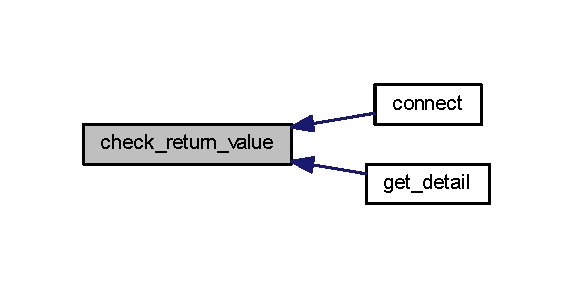
\includegraphics[width=275pt]{classceus__importer_a9147e757eb1c4c80e2720b160b86c239_icgraph}
\end{center}
\end{figure}


\hypertarget{classceus__importer_a5cd89fd2b1560b25eb4300ea6662a1b7}{\index{ceus\+\_\+importer@{ceus\+\_\+importer}!check\+\_\+vocabulary@{check\+\_\+vocabulary}}
\index{check\+\_\+vocabulary@{check\+\_\+vocabulary}!ceus\+\_\+importer@{ceus\+\_\+importer}}
\paragraph[{check\+\_\+vocabulary}]{\setlength{\rightskip}{0pt plus 5cm}check\+\_\+vocabulary (
\begin{DoxyParamCaption}
\item[{}]{\$a\+Curriculum}
\end{DoxyParamCaption}
)\hspace{0.3cm}{\ttfamily [private]}}}\label{classceus__importer_a5cd89fd2b1560b25eb4300ea6662a1b7}


Checks if a taxonomy vocabulary for the given curriculum exists and creates it if not. 

This function stores the corresponding vocabulary (either a new or an existing one) into the \hyperlink{classceus__importer_a84266bdaf38a24150ceb43d88ebb230d}{\$a\+Vocabulary} array.

\begin{DoxyRemark}{Remarks}
This method creates the new vocabulary with the default weight of {\ttfamily 10}, but only vocabularies with a weight below {\ttfamily 0} will be shown publicly.
\end{DoxyRemark}

\begin{DoxyParams}[1]{Parameters}
array & {\em \$a\+Curriculum} & Curriculum from C\+E\+U\+S as returned by \hyperlink{classceus__importer_a16485f39c6678a011ff758e76bf1f458}{get\+\_\+curricula\+\_\+list()}\\
\hline
\end{DoxyParams}
\begin{DoxyAuthor}{Author}
Konstantinos Dafalias -\/ \href{mailto:kdafalias@gmail.com}{\tt kdafalias@gmail.\+com} 
\end{DoxyAuthor}
\begin{DoxyVersion}{Version}
1.\+0.\+0 2014-\/07-\/16 
\end{DoxyVersion}
\begin{DoxySince}{Since}
Commit \href{http://github.com/TheJake123/DrupalModul/commit/d179abcc5e05743086cd67cf1ce30b08923a7183}{\tt d179abc} on 2014-\/06-\/28 
\end{DoxySince}


Definition at line 727 of file ceus\+\_\+importer.\+inc.\+php.

\hypertarget{classceus__importer_a78572828d11dcdf2a498497d9001d557}{\index{ceus\+\_\+importer@{ceus\+\_\+importer}!connect@{connect}}
\index{connect@{connect}!ceus\+\_\+importer@{ceus\+\_\+importer}}
\paragraph[{connect}]{\setlength{\rightskip}{0pt plus 5cm}connect (
\begin{DoxyParamCaption}
{}
\end{DoxyParamCaption}
)}}\label{classceus__importer_a78572828d11dcdf2a498497d9001d557}


Connect to C\+E\+U\+S and receive Authtoken. 

This function tries to connect to the C\+E\+U\+S-\/\+A\+P\+I server and receives and stores the authtoken. Returns true if an authtoken was recieved otherwise it returns false.


\begin{DoxyRetVals}{Return values}
{\em true} & Connection and authentication {\bfseries successful} \\
\hline
{\em false} & Connection and/or authentication {\bfseries failed} \\
\hline
\end{DoxyRetVals}
\begin{DoxyAuthor}{Author}
Konstantinos Dafalias -\/ \href{mailto:kdafalias@gmail.com}{\tt kdafalias@gmail.\+com} 
\end{DoxyAuthor}
\begin{DoxyVersion}{Version}
1.\+0.\+0 2014-\/07-\/16 
\end{DoxyVersion}
\begin{DoxySince}{Since}
Commit \href{http://github.com/TheJake123/DrupalModul/commit/d179abcc5e05743086cd67cf1ce30b08923a7183}{\tt d179abc} on 2014-\/06-\/28 
\end{DoxySince}


Definition at line 247 of file ceus\+\_\+importer.\+inc.\+php.



References check\+\_\+return\+\_\+value().



Here is the call graph for this function\+:
\nopagebreak
\begin{figure}[H]
\begin{center}
\leavevmode
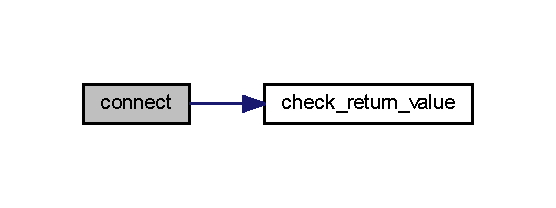
\includegraphics[width=267pt]{classceus__importer_a78572828d11dcdf2a498497d9001d557_cgraph}
\end{center}
\end{figure}


\hypertarget{classceus__importer_a9b4d3aec74218c3b3ea4fd6b2dabec17}{\index{ceus\+\_\+importer@{ceus\+\_\+importer}!find\+\_\+nodeid\+\_\+by\+\_\+field@{find\+\_\+nodeid\+\_\+by\+\_\+field}}
\index{find\+\_\+nodeid\+\_\+by\+\_\+field@{find\+\_\+nodeid\+\_\+by\+\_\+field}!ceus\+\_\+importer@{ceus\+\_\+importer}}
\paragraph[{find\+\_\+nodeid\+\_\+by\+\_\+field}]{\setlength{\rightskip}{0pt plus 5cm}find\+\_\+nodeid\+\_\+by\+\_\+field (
\begin{DoxyParamCaption}
\item[{}]{\$s\+Fieldtype, }
\item[{}]{\$s\+Fieldcontent}
\end{DoxyParamCaption}
)\hspace{0.3cm}{\ttfamily [private]}}}\label{classceus__importer_a9b4d3aec74218c3b3ea4fd6b2dabec17}


Looks for Drupal content node by title or code. 

This function searches for the Drupal content node corresponding to a given course code or course title.


\begin{DoxyParams}[1]{Parameters}
string & {\em \$s\+Fieldtype} & The name of the field to search in. This can be either \char`\"{}code\char`\"{} or \char`\"{}title\char`\"{}. \\
\hline
string & {\em \$s\+Fieldcontent} & The search term to look for \\
\hline
\end{DoxyParams}

\begin{DoxyRetVals}{Return values}
{\em nid} & The node's id \\
\hline
{\em false} & No content node with this title or code could be found\\
\hline
\end{DoxyRetVals}
\begin{DoxyAuthor}{Author}
Konstantinos Dafalias -\/ \href{mailto:kdafalias@gmail.com}{\tt kdafalias@gmail.\+com} 
\end{DoxyAuthor}
\begin{DoxyVersion}{Version}
1.\+0.\+0 2014-\/07-\/16 
\end{DoxyVersion}
\begin{DoxySince}{Since}
Commit \href{http://github.com/TheJake123/DrupalModul/commit/d179abcc5e05743086cd67cf1ce30b08923a7183}{\tt d179abc} on 2014-\/06-\/28
\end{DoxySince}
\begin{DoxySeeAlso}{See also}
\hyperlink{classceus__importer_acc5550c279b1a38aac4ee7fe0680e14d}{get\+\_\+term\+\_\+ids()} 
\end{DoxySeeAlso}


Definition at line 450 of file ceus\+\_\+importer.\+inc.\+php.

\hypertarget{classceus__importer_abd2f9a9afc073169b2badcb571cc983c}{\index{ceus\+\_\+importer@{ceus\+\_\+importer}!get\+\_\+curricula@{get\+\_\+curricula}}
\index{get\+\_\+curricula@{get\+\_\+curricula}!ceus\+\_\+importer@{ceus\+\_\+importer}}
\paragraph[{get\+\_\+curricula}]{\setlength{\rightskip}{0pt plus 5cm}get\+\_\+curricula (
\begin{DoxyParamCaption}
{}
\end{DoxyParamCaption}
)}}\label{classceus__importer_abd2f9a9afc073169b2badcb571cc983c}


Main method\+: Imports curriculum data from C\+E\+U\+S. 

This is the main public method of this class. It does the following things\+:
\begin{DoxyEnumerate}
\item Reset the statistics
\item Imports all curricula
\item Create a new vocabulary if none exists
\item Load course data from C\+E\+U\+S A\+P\+I
\item Process relations
\item Store everything into the Drupal database
\end{DoxyEnumerate}


\begin{DoxyRetVals}{Return values}
{\em success message} & The import was successful. This message contains the \hyperlink{classceus__importer_ac383d13daab8093b15c3925f305d8c08}{import statistics}. \\
\hline
{\em false} & An error has occured and the import was not successful.\\
\hline
\end{DoxyRetVals}
\begin{DoxyAuthor}{Authors}
Konstantinos Dafalias -\/ \href{mailto:kdafalias@gmail.com}{\tt kdafalias@gmail.\+com} 
\end{DoxyAuthor}
\begin{DoxyAuthor}{Author}
Jakob Strasser -\/ \href{mailto:jakob.strasser@telenet.be}{\tt jakob.\+strasser@telenet.\+be} 
\end{DoxyAuthor}
\begin{DoxyVersion}{Version}
1.\+0.\+0 2014-\/07-\/16 
\end{DoxyVersion}
\begin{DoxySince}{Since}
Commit \href{http://github.com/TheJake123/DrupalModul/commit/d179abcc5e05743086cd67cf1ce30b08923a7183}{\tt d179abc} on 2014-\/06-\/28
\end{DoxySince}
\begin{DoxySeeAlso}{See also}
\hyperlink{classceus__importer_a16485f39c6678a011ff758e76bf1f458}{get\+\_\+curricula\+\_\+list()} 

\hyperlink{classceus__importer_a5cd89fd2b1560b25eb4300ea6662a1b7}{check\+\_\+vocabulary()} 

\hyperlink{classceus__importer_a0282b9b18ad499198f75d6d81fc82ad0}{get\+\_\+curriculum()} 

\hyperlink{classceus__importer_a404368bea7498901cfdc0fca559089b6}{get\+\_\+details()} 

\hyperlink{classceus__importer_a04b7723caf55a2cfd4b92d02754748dc}{process\+\_\+relations()} 
\end{DoxySeeAlso}


Definition at line 691 of file ceus\+\_\+importer.\+inc.\+php.

\hypertarget{classceus__importer_a16485f39c6678a011ff758e76bf1f458}{\index{ceus\+\_\+importer@{ceus\+\_\+importer}!get\+\_\+curricula\+\_\+list@{get\+\_\+curricula\+\_\+list}}
\index{get\+\_\+curricula\+\_\+list@{get\+\_\+curricula\+\_\+list}!ceus\+\_\+importer@{ceus\+\_\+importer}}
\paragraph[{get\+\_\+curricula\+\_\+list}]{\setlength{\rightskip}{0pt plus 5cm}get\+\_\+curricula\+\_\+list (
\begin{DoxyParamCaption}
{}
\end{DoxyParamCaption}
)\hspace{0.3cm}{\ttfamily [private]}}}\label{classceus__importer_a16485f39c6678a011ff758e76bf1f458}


Gets a list of all curricula (bachelor, master) from C\+E\+U\+S. 

This function retreives a list of all available curricula from the C\+E\+U\+S A\+P\+I.

\begin{DoxyReturn}{Returns}
Associative array containing all curricula
\end{DoxyReturn}
\begin{DoxyAuthor}{Author}
Konstantinos Dafalias -\/ \href{mailto:kdafalias@gmail.com}{\tt kdafalias@gmail.\+com} 
\end{DoxyAuthor}
\begin{DoxyVersion}{Version}
1.\+0.\+0 2014-\/07-\/16 
\end{DoxyVersion}
\begin{DoxySince}{Since}
Commit \href{http://github.com/TheJake123/DrupalModul/commit/d179abcc5e05743086cd67cf1ce30b08923a7183}{\tt d179abc} on 2014-\/06-\/28 
\end{DoxySince}


Definition at line 769 of file ceus\+\_\+importer.\+inc.\+php.

\hypertarget{classceus__importer_a0282b9b18ad499198f75d6d81fc82ad0}{\index{ceus\+\_\+importer@{ceus\+\_\+importer}!get\+\_\+curriculum@{get\+\_\+curriculum}}
\index{get\+\_\+curriculum@{get\+\_\+curriculum}!ceus\+\_\+importer@{ceus\+\_\+importer}}
\paragraph[{get\+\_\+curriculum}]{\setlength{\rightskip}{0pt plus 5cm}get\+\_\+curriculum (
\begin{DoxyParamCaption}
\item[{}]{\$i\+I\+D}
\end{DoxyParamCaption}
)\hspace{0.3cm}{\ttfamily [private]}}}\label{classceus__importer_a0282b9b18ad499198f75d6d81fc82ad0}


Gets one curriculum tree from C\+E\+U\+S. 

This function retreives the complete tree of one certain curriculum from the C\+E\+U\+S A\+P\+I


\begin{DoxyParams}[1]{Parameters}
integer & {\em \$i\+I\+D} & C\+E\+U\+S id of the curriculum \\
\hline
\end{DoxyParams}
\begin{DoxyReturn}{Returns}
Nested array of course ids
\end{DoxyReturn}
\begin{DoxyAuthor}{Author}
Konstantinos Dafalias -\/ \href{mailto:kdafalias@gmail.com}{\tt kdafalias@gmail.\+com} 
\end{DoxyAuthor}
\begin{DoxyVersion}{Version}
1.\+0.\+0 2014-\/07-\/16 
\end{DoxyVersion}
\begin{DoxySince}{Since}
Commit \href{http://github.com/TheJake123/DrupalModul/commit/d179abcc5e05743086cd67cf1ce30b08923a7183}{\tt d179abc} on 2014-\/06-\/28 
\end{DoxySince}


Definition at line 787 of file ceus\+\_\+importer.\+inc.\+php.

\hypertarget{classceus__importer_a1b7d86575274b687d8e2fa9b29d7f7ba}{\index{ceus\+\_\+importer@{ceus\+\_\+importer}!get\+\_\+detail@{get\+\_\+detail}}
\index{get\+\_\+detail@{get\+\_\+detail}!ceus\+\_\+importer@{ceus\+\_\+importer}}
\paragraph[{get\+\_\+detail}]{\setlength{\rightskip}{0pt plus 5cm}get\+\_\+detail (
\begin{DoxyParamCaption}
\item[{}]{\$i\+I\+D}
\end{DoxyParamCaption}
)\hspace{0.3cm}{\ttfamily [private]}}}\label{classceus__importer_a1b7d86575274b687d8e2fa9b29d7f7ba}


Fetches a single course from C\+E\+U\+S. 

This function fetches a single course from the C\+E\+U\+S A\+P\+I and returns all its details in an array.


\begin{DoxyParams}[1]{Parameters}
integer & {\em \$i\+I\+D} & C\+E\+U\+S id of the course\\
\hline
\end{DoxyParams}

\begin{DoxyRetVals}{Return values}
{\em details} & 2-\/dimensional array containing the course details. 1. dimension = language, 2. dimension = details. \\
\hline
{\em false} & An error occured while fetching the details\\
\hline
\end{DoxyRetVals}
\begin{DoxyAuthor}{Authors}
Konstantinos Dafalias -\/ \href{mailto:kdafalias@gmail.com}{\tt kdafalias@gmail.\+com} 

Jakob Strasser -\/ \href{mailto:jakob.strasser@telenet.be}{\tt jakob.\+strasser@telenet.\+be} 
\end{DoxyAuthor}
\begin{DoxyVersion}{Version}
1.\+0.\+0 2014-\/07-\/16 
\end{DoxyVersion}
\begin{DoxySince}{Since}
Commit \href{http://github.com/TheJake123/DrupalModul/commit/d179abcc5e05743086cd67cf1ce30b08923a7183}{\tt d179abc} on 2014-\/06-\/28
\end{DoxySince}
\begin{DoxySeeAlso}{See also}
\hyperlink{classceus__importer_a404368bea7498901cfdc0fca559089b6}{get\+\_\+details()} 
\end{DoxySeeAlso}


Definition at line 274 of file ceus\+\_\+importer.\+inc.\+php.



References check\+\_\+return\+\_\+value().



Here is the call graph for this function\+:
\nopagebreak
\begin{figure}[H]
\begin{center}
\leavevmode
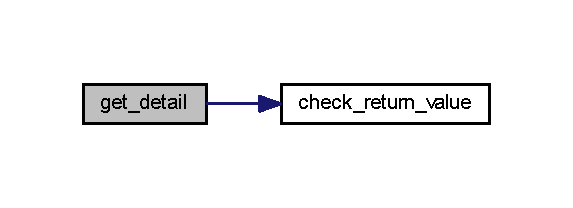
\includegraphics[width=275pt]{classceus__importer_a1b7d86575274b687d8e2fa9b29d7f7ba_cgraph}
\end{center}
\end{figure}


\hypertarget{classceus__importer_a404368bea7498901cfdc0fca559089b6}{\index{ceus\+\_\+importer@{ceus\+\_\+importer}!get\+\_\+details@{get\+\_\+details}}
\index{get\+\_\+details@{get\+\_\+details}!ceus\+\_\+importer@{ceus\+\_\+importer}}
\paragraph[{get\+\_\+details}]{\setlength{\rightskip}{0pt plus 5cm}get\+\_\+details (
\begin{DoxyParamCaption}
\item[{}]{\$a\+Tree, }
\item[{}]{\$i\+Parent\+I\+D, }
\item[{}]{\$i\+Curriculum\+I\+D}
\end{DoxyParamCaption}
)\hspace{0.3cm}{\ttfamily [private]}}}\label{classceus__importer_a404368bea7498901cfdc0fca559089b6}


Recursive function that traverses a curriculum tree. 

This method goes through all the courses of a curriculum that have been returned by C\+E\+U\+S recursively and reads the details for each course into the \hyperlink{classceus__importer_a504ee22f4791f6d41ebe97c5786ee547}{\$a\+Terms} array. A vocabulary term is created for each item in the respective curriculum.


\begin{DoxyParams}[1]{Parameters}
array & {\em \$a\+Tree} & The current subtree in the curriculum \\
\hline
integer & {\em \$i\+Parent\+I\+D} & Drupal term id of this course's parent term \\
\hline
integer & {\em \$i\+Curriculum\+I\+D} & C\+E\+U\+S id of the curriculum this tree belongs to \\
\hline
\end{DoxyParams}

\begin{DoxyRetVals}{Return values}
{\em true} & Courses have been read \\
\hline
{\em false} & The subtree has reached a leaf\\
\hline
\end{DoxyRetVals}
\begin{DoxyAuthor}{Author}
Konstantinos Dafalias -\/ \href{mailto:kdafalias@gmail.com}{\tt kdafalias@gmail.\+com} 
\end{DoxyAuthor}
\begin{DoxyVersion}{Version}
1.\+0.\+0 2014-\/07-\/16 
\end{DoxyVersion}
\begin{DoxySince}{Since}
Commit \href{http://github.com/TheJake123/DrupalModul/commit/d179abcc5e05743086cd67cf1ce30b08923a7183}{\tt d179abc} on 2014-\/06-\/28
\end{DoxySince}
\begin{DoxySeeAlso}{See also}
\hyperlink{classceus__importer_a1b7d86575274b687d8e2fa9b29d7f7ba}{get\+\_\+detail()} 
\end{DoxySeeAlso}


Definition at line 638 of file ceus\+\_\+importer.\+inc.\+php.

\hypertarget{classceus__importer_a1c0091515372f72e1a87683ca57c74eb}{\index{ceus\+\_\+importer@{ceus\+\_\+importer}!get\+\_\+error@{get\+\_\+error}}
\index{get\+\_\+error@{get\+\_\+error}!ceus\+\_\+importer@{ceus\+\_\+importer}}
\paragraph[{get\+\_\+error}]{\setlength{\rightskip}{0pt plus 5cm}get\+\_\+error (
\begin{DoxyParamCaption}
{}
\end{DoxyParamCaption}
)}}\label{classceus__importer_a1c0091515372f72e1a87683ca57c74eb}


Returns last error message. 

This function acts as a public getter for the \hyperlink{classceus__importer_a92ce9963d72f9742e6e7051b23c478b6}{error message}.

\begin{DoxyReturn}{Returns}
string 
\end{DoxyReturn}
\begin{DoxyAuthor}{Author}
Konstantinos Dafalias -\/ \href{mailto:kdafalias@gmail.com}{\tt kdafalias@gmail.\+com} 
\end{DoxyAuthor}
\begin{DoxyVersion}{Version}
1.\+0.\+0 2014-\/07-\/16 
\end{DoxyVersion}
\begin{DoxySince}{Since}
Commit \href{http://github.com/TheJake123/DrupalModul/commit/d179abcc5e05743086cd67cf1ce30b08923a7183}{\tt d179abc} on 2014-\/06-\/28
\end{DoxySince}
\begin{DoxySeeAlso}{See also}
\hyperlink{classceus__importer_a92ce9963d72f9742e6e7051b23c478b6}{\$s\+Error} 
\end{DoxySeeAlso}


Definition at line 804 of file ceus\+\_\+importer.\+inc.\+php.

\hypertarget{classceus__importer_acc5550c279b1a38aac4ee7fe0680e14d}{\index{ceus\+\_\+importer@{ceus\+\_\+importer}!get\+\_\+term\+\_\+ids@{get\+\_\+term\+\_\+ids}}
\index{get\+\_\+term\+\_\+ids@{get\+\_\+term\+\_\+ids}!ceus\+\_\+importer@{ceus\+\_\+importer}}
\paragraph[{get\+\_\+term\+\_\+ids}]{\setlength{\rightskip}{0pt plus 5cm}get\+\_\+term\+\_\+ids (
\begin{DoxyParamCaption}
\item[{}]{\$s\+Relationfield}
\end{DoxyParamCaption}
)\hspace{0.3cm}{\ttfamily [private]}}}\label{classceus__importer_acc5550c279b1a38aac4ee7fe0680e14d}


Parses the {\ttfamily voraussetzungen} field of a course and tries to extract the relation. 

This function loops through all links and list items in the {\ttfamily voraussetzugnen} field and tries to extracts the referenced courses. It does this in 3 steps\+:
\begin{DoxyEnumerate}
\item Extract the course names
\item Try to get the Drupal content node id through the course title
\item Try to get the Drupal content node id through the course code
\end{DoxyEnumerate}


\begin{DoxyParams}[1]{Parameters}
string & {\em \$s\+Relationfield} & Textual content of the {\ttfamily voraussetzungen} field as received from C\+E\+U\+S \\
\hline
\end{DoxyParams}
\begin{DoxyReturn}{Returns}
Drupal content node ids of related courses
\end{DoxyReturn}
\begin{DoxyAuthor}{Author}
Konstantinos Dafalias -\/ \href{mailto:kdafalias@gmail.com}{\tt kdafalias@gmail.\+com} 
\end{DoxyAuthor}
\begin{DoxyVersion}{Version}
1.\+0.\+0 2014-\/07-\/16 
\end{DoxyVersion}
\begin{DoxySince}{Since}
Commit \href{http://github.com/TheJake123/DrupalModul/commit/d179abcc5e05743086cd67cf1ce30b08923a7183}{\tt d179abc} on 2014-\/06-\/28
\end{DoxySince}
\begin{DoxySeeAlso}{See also}
\hyperlink{classceus__importer_a9b4d3aec74218c3b3ea4fd6b2dabec17}{find\+\_\+nodeid\+\_\+by\+\_\+field()} 

\hyperlink{classceus__importer_a49143005c3d0328fd8e982f2f035f9e0}{parse\+\_\+link\+\_\+term\+\_\+code()} 
\end{DoxySeeAlso}


Definition at line 486 of file ceus\+\_\+importer.\+inc.\+php.

\hypertarget{classceus__importer_a689c3df400e042323dcfc8a70bb86c0e}{\index{ceus\+\_\+importer@{ceus\+\_\+importer}!has\+\_\+relation@{has\+\_\+relation}}
\index{has\+\_\+relation@{has\+\_\+relation}!ceus\+\_\+importer@{ceus\+\_\+importer}}
\paragraph[{has\+\_\+relation}]{\setlength{\rightskip}{0pt plus 5cm}has\+\_\+relation (
\begin{DoxyParamCaption}
\item[{}]{\$s\+Relationfield}
\end{DoxyParamCaption}
)\hspace{0.3cm}{\ttfamily [private]}}}\label{classceus__importer_a689c3df400e042323dcfc8a70bb86c0e}


Checks if a course has recommendations or prerequisites. 

This function determines if a course has a relation with another course. This is the case when the {\itshape \$s\+Relationfield} is not empty and does not begin with \char`\"{}kein\char`\"{} (case insensitive). Returns true if there are any relations that need to be processed. Return false if the arent any.


\begin{DoxyParams}[1]{Parameters}
string & {\em \$s\+Relationfield} & Content of the courses {\ttfamily voraussetzungen} field\\
\hline
\end{DoxyParams}

\begin{DoxyRetVals}{Return values}
{\em true} & The course has recommendations or prerequisites \\
\hline
{\em false} & The course does {\bfseries not} have recommendations or prerequisites\\
\hline
\end{DoxyRetVals}
\begin{DoxyAuthor}{Author}
Konstantinos Dafalias -\/ \href{mailto:kdafalias@gmail.com}{\tt kdafalias@gmail.\+com} 
\end{DoxyAuthor}
\begin{DoxyVersion}{Version}
1.\+0.\+0 2014-\/07-\/16 
\end{DoxyVersion}
\begin{DoxySince}{Since}
Commit \href{http://github.com/TheJake123/DrupalModul/commit/d179abcc5e05743086cd67cf1ce30b08923a7183}{\tt d179abc} on 2014-\/06-\/28 
\end{DoxySince}


Definition at line 404 of file ceus\+\_\+importer.\+inc.\+php.

\hypertarget{classceus__importer_a49143005c3d0328fd8e982f2f035f9e0}{\index{ceus\+\_\+importer@{ceus\+\_\+importer}!parse\+\_\+link\+\_\+term\+\_\+code@{parse\+\_\+link\+\_\+term\+\_\+code}}
\index{parse\+\_\+link\+\_\+term\+\_\+code@{parse\+\_\+link\+\_\+term\+\_\+code}!ceus\+\_\+importer@{ceus\+\_\+importer}}
\paragraph[{parse\+\_\+link\+\_\+term\+\_\+code}]{\setlength{\rightskip}{0pt plus 5cm}parse\+\_\+link\+\_\+term\+\_\+code (
\begin{DoxyParamCaption}
\item[{}]{\$s\+Link}
\end{DoxyParamCaption}
)\hspace{0.3cm}{\ttfamily [private]}}}\label{classceus__importer_a49143005c3d0328fd8e982f2f035f9e0}


Parses linked web page and tries to extract a course code. 

This function tries to extract the course code (e.\+g. {\itshape 1\+F\+E\+N\+K\+F}) from website behind the given {\itshape \$s\+Link} and returns it.


\begin{DoxyParams}[1]{Parameters}
string & {\em \$s\+Link} & H\+T\+M\+L-\/\+Code with Link to C\+E\+U\+S entry \\
\hline
\end{DoxyParams}

\begin{DoxyRetVals}{Return values}
{\em course code} & The extracted code \\
\hline
{\em false} & The extraction was not successful\\
\hline
\end{DoxyRetVals}
\begin{DoxyAuthor}{Author}
Konstantinos Dafalias -\/ \href{mailto:kdafalias@gmail.com}{\tt kdafalias@gmail.\+com} 
\end{DoxyAuthor}
\begin{DoxyVersion}{Version}
1.\+0.\+0 2014-\/07-\/16 
\end{DoxyVersion}
\begin{DoxySince}{Since}
Commit \href{http://github.com/TheJake123/DrupalModul/commit/d179abcc5e05743086cd67cf1ce30b08923a7183}{\tt d179abc} on 2014-\/06-\/28 
\end{DoxySince}
\begin{DoxySeeAlso}{See also}
\hyperlink{classceus__importer_acc5550c279b1a38aac4ee7fe0680e14d}{get\+\_\+term\+\_\+ids()} 
\end{DoxySeeAlso}


Definition at line 423 of file ceus\+\_\+importer.\+inc.\+php.

\hypertarget{classceus__importer_a04b7723caf55a2cfd4b92d02754748dc}{\index{ceus\+\_\+importer@{ceus\+\_\+importer}!process\+\_\+relations@{process\+\_\+relations}}
\index{process\+\_\+relations@{process\+\_\+relations}!ceus\+\_\+importer@{ceus\+\_\+importer}}
\paragraph[{process\+\_\+relations}]{\setlength{\rightskip}{0pt plus 5cm}process\+\_\+relations (
\begin{DoxyParamCaption}
{}
\end{DoxyParamCaption}
)\hspace{0.3cm}{\ttfamily [private]}}}\label{classceus__importer_a04b7723caf55a2cfd4b92d02754748dc}


Creates Drupal relations out of C\+E\+U\+S relations. 

This procedure loops through \hyperlink{classceus__importer_a112b3b5ddcf754007f9466ec5ab94683}{\$a\+Relations}, parses the {\ttfamily voraussetzungen} field of each course, generates relations for required and suggested courses and stores them in the node

\begin{DoxyAuthor}{Author}
Konstantinos Dafalias -\/ \href{mailto:kdafalias@gmail.com}{\tt kdafalias@gmail.\+com} 
\end{DoxyAuthor}
\begin{DoxyVersion}{Version}
1.\+0.\+0 2014-\/07-\/16 
\end{DoxyVersion}
\begin{DoxySince}{Since}
Commit \href{http://github.com/TheJake123/DrupalModul/commit/d179abcc5e05743086cd67cf1ce30b08923a7183}{\tt d179abc} on 2014-\/06-\/28
\end{DoxySince}
\begin{DoxySeeAlso}{See also}
\hyperlink{classceus__importer_acc5550c279b1a38aac4ee7fe0680e14d}{get\+\_\+term\+\_\+ids()} 
\end{DoxySeeAlso}


Definition at line 534 of file ceus\+\_\+importer.\+inc.\+php.

\hypertarget{classceus__importer_ae963f27a37b0a77da7c6f6c936625d3c}{\index{ceus\+\_\+importer@{ceus\+\_\+importer}!save\+\_\+node@{save\+\_\+node}}
\index{save\+\_\+node@{save\+\_\+node}!ceus\+\_\+importer@{ceus\+\_\+importer}}
\paragraph[{save\+\_\+node}]{\setlength{\rightskip}{0pt plus 5cm}save\+\_\+node (
\begin{DoxyParamCaption}
\item[{}]{\$a\+Detail, }
\item[{}]{\$tid}
\end{DoxyParamCaption}
)\hspace{0.3cm}{\ttfamily [private]}}}\label{classceus__importer_ae963f27a37b0a77da7c6f6c936625d3c}


Saves a course as a Drupal content node. 

If a node already exists, the function checks if the changedate has changed. If so, a new version of this conent node is created. If not, nothing is changed


\begin{DoxyParams}[1]{Parameters}
array & {\em \$a\+Detail} & Array of course details as returned by \hyperlink{classceus__importer_a1b7d86575274b687d8e2fa9b29d7f7ba}{get\+\_\+detail()} \\
\hline
array & {\em \$tid} & Drupal vocabulary term id of the vocabulary term corresponding to the given course \\
\hline
\end{DoxyParams}
\begin{DoxyReturn}{Returns}
Node id of the saved content node
\end{DoxyReturn}
\begin{DoxyAuthor}{Author}
Konstantinos Dafalias -\/ \href{mailto:kdafalias@gmail.com}{\tt kdafalias@gmail.\+com} 
\end{DoxyAuthor}
\begin{DoxyAuthor}{Authors}
Jakob Strasser -\/ \href{mailto:jakob.strasser@telenet.be}{\tt jakob.\+strasser@telenet.\+be} 
\end{DoxyAuthor}
\begin{DoxyVersion}{Version}
1.\+0.\+0 2014-\/07-\/16 
\end{DoxyVersion}
\begin{DoxySince}{Since}
Commit \href{http://github.com/TheJake123/DrupalModul/commit/d179abcc5e05743086cd67cf1ce30b08923a7183}{\tt d179abc} on 2014-\/06-\/28 
\end{DoxySince}


Definition at line 308 of file ceus\+\_\+importer.\+inc.\+php.



\subsubsection{Field Documentation}
\hypertarget{classceus__importer_ad7deba772fa82f6de2343032ac86a5b5}{\index{ceus\+\_\+importer@{ceus\+\_\+importer}!\$a\+Files@{\$a\+Files}}
\index{\$a\+Files@{\$a\+Files}!ceus\+\_\+importer@{ceus\+\_\+importer}}
\paragraph[{\$a\+Files}]{\setlength{\rightskip}{0pt plus 5cm}\$a\+Files\hspace{0.3cm}{\ttfamily [private]}}}\label{classceus__importer_ad7deba772fa82f6de2343032ac86a5b5}
{\bfseries Initial value\+:}
\begin{DoxyCode}
= array (
            \textcolor{stringliteral}{'AUTH'} => \textcolor{stringliteral}{'auth.php'},
            \textcolor{stringliteral}{'LIST'} => \textcolor{stringliteral}{'list.php'},
            \textcolor{stringliteral}{'CURR'} => \textcolor{stringliteral}{'curr.php'},
            \textcolor{stringliteral}{'DETAIL'} => \textcolor{stringliteral}{'detail.php'} 
    )
\end{DoxyCode}


Names of the A\+P\+I methods. 

This array contains all the A\+P\+I method names for\+:
\begin{DoxyItemize}
\item Getting an authorization token
\item Listing all curricula
\item Getting one curriculum tree
\item Getting one curriculum item
\end{DoxyItemize}

\begin{DoxyAuthor}{Author}
Konstantinos Dafalias -\/ \href{mailto:kdafalias@gmail.com}{\tt kdafalias@gmail.\+com} 
\end{DoxyAuthor}
\begin{DoxySince}{Since}
Commit \href{http://github.com/TheJake123/DrupalModul/commit/d179abcc5e05743086cd67cf1ce30b08923a7183}{\tt d179abc} on 2014-\/06-\/28 
\end{DoxySince}


Definition at line 102 of file ceus\+\_\+importer.\+inc.\+php.

\hypertarget{classceus__importer_a87139169928b8a390915f5962c56f814}{\index{ceus\+\_\+importer@{ceus\+\_\+importer}!\$a\+Language@{\$a\+Language}}
\index{\$a\+Language@{\$a\+Language}!ceus\+\_\+importer@{ceus\+\_\+importer}}
\paragraph[{\$a\+Language}]{\setlength{\rightskip}{0pt plus 5cm}\$a\+Language\hspace{0.3cm}{\ttfamily [private]}}}\label{classceus__importer_a87139169928b8a390915f5962c56f814}
{\bfseries Initial value\+:}
\begin{DoxyCode}
= array (
            \textcolor{stringliteral}{'de'},
            \textcolor{stringliteral}{'en'} 
    )
\end{DoxyCode}


All supported languages. 

This array contains the short names of all languages that should be imported.

\begin{DoxyAuthor}{Author}
Konstantinos Dafalias -\/ \href{mailto:kdafalias@gmail.com}{\tt kdafalias@gmail.\+com} 
\end{DoxyAuthor}
\begin{DoxySince}{Since}
Commit \href{http://github.com/TheJake123/DrupalModul/commit/d179abcc5e05743086cd67cf1ce30b08923a7183}{\tt d179abc} on 2014-\/06-\/28 
\end{DoxySince}


Definition at line 127 of file ceus\+\_\+importer.\+inc.\+php.

\hypertarget{classceus__importer_a112b3b5ddcf754007f9466ec5ab94683}{\index{ceus\+\_\+importer@{ceus\+\_\+importer}!\$a\+Relations@{\$a\+Relations}}
\index{\$a\+Relations@{\$a\+Relations}!ceus\+\_\+importer@{ceus\+\_\+importer}}
\paragraph[{\$a\+Relations}]{\setlength{\rightskip}{0pt plus 5cm}\$a\+Relations\hspace{0.3cm}{\ttfamily [private]}}}\label{classceus__importer_a112b3b5ddcf754007f9466ec5ab94683}


Relations of every course (if available) 

This array contains all relations (recommended and needed) in their raw textual form It is filled during the import and evaluated at the end.

The key is the C\+E\+U\+S id of the cours, the value contains the content text of the {\ttfamily voraussetzungen} field from C\+E\+U\+S.

\begin{DoxyAuthor}{Author}
Konstantinos Dafalias -\/ \href{mailto:kdafalias@gmail.com}{\tt kdafalias@gmail.\+com} 
\end{DoxyAuthor}
\begin{DoxySince}{Since}
Commit \href{http://github.com/TheJake123/DrupalModul/commit/d179abcc5e05743086cd67cf1ce30b08923a7183}{\tt d179abc} on 2014-\/06-\/28 
\end{DoxySince}


Definition at line 186 of file ceus\+\_\+importer.\+inc.\+php.

\hypertarget{classceus__importer_ac383d13daab8093b15c3925f305d8c08}{\index{ceus\+\_\+importer@{ceus\+\_\+importer}!\$a\+Stats@{\$a\+Stats}}
\index{\$a\+Stats@{\$a\+Stats}!ceus\+\_\+importer@{ceus\+\_\+importer}}
\paragraph[{\$a\+Stats}]{\setlength{\rightskip}{0pt plus 5cm}\$a\+Stats\hspace{0.3cm}{\ttfamily [private]}}}\label{classceus__importer_ac383d13daab8093b15c3925f305d8c08}
{\bfseries Initial value\+:}
\begin{DoxyCode}
= array (
            \textcolor{stringliteral}{'loaded'} => 0,
            \textcolor{stringliteral}{'new'} => 0,
            \textcolor{stringliteral}{'updated'} => 0,
            \textcolor{stringliteral}{'numcurrs'} => 0,
            \textcolor{stringliteral}{'relations'} => 0 
    )
\end{DoxyCode}


Import statistics. 

This array contains all necessary import statistics, namely\+:
\begin{DoxyItemize}
\item The number of courses loaded from C\+E\+U\+S
\item The number of new content nodes created (= new courses)
\item The number of content nodes that were updated during the import (= changes in C\+E\+U\+S)
\item The number of curricula loaded from C\+E\+U\+S
\item the number of relations automatically processed
\end{DoxyItemize}

\begin{DoxyAuthor}{Author}
Jakob Strasser -\/ \href{mailto:jakob.strasser@telenet.be}{\tt jakob.\+strasser@telenet.\+be} 
\end{DoxyAuthor}
\begin{DoxySince}{Since}
Commit \href{http://github.com/TheJake123/DrupalModul/commit/5ad002c8e7a233bc25ac0e1dcf2b9f62520281c1}{\tt 5ad002c} on 2014-\/07-\/08 
\end{DoxySince}


Definition at line 167 of file ceus\+\_\+importer.\+inc.\+php.

\hypertarget{classceus__importer_a504ee22f4791f6d41ebe97c5786ee547}{\index{ceus\+\_\+importer@{ceus\+\_\+importer}!\$a\+Terms@{\$a\+Terms}}
\index{\$a\+Terms@{\$a\+Terms}!ceus\+\_\+importer@{ceus\+\_\+importer}}
\paragraph[{\$a\+Terms}]{\setlength{\rightskip}{0pt plus 5cm}\$a\+Terms\hspace{0.3cm}{\ttfamily [private]}}}\label{classceus__importer_a504ee22f4791f6d41ebe97c5786ee547}


All Terms for vocabularies. 

This array contains all the Drupal vocabulary terms associated with the curriculum currently being processed.

The item key represents the C\+E\+U\+S id of one course.

\begin{DoxyAuthor}{Author}
Konstantinos Dafalias -\/ \href{mailto:kdafalias@gmail.com}{\tt kdafalias@gmail.\+com} 
\end{DoxyAuthor}
\begin{DoxySince}{Since}
Commit \href{http://github.com/TheJake123/DrupalModul/commit/d179abcc5e05743086cd67cf1ce30b08923a7183}{\tt d179abc} on 2014-\/06-\/28 
\end{DoxySince}


Definition at line 152 of file ceus\+\_\+importer.\+inc.\+php.

\hypertarget{classceus__importer_a84266bdaf38a24150ceb43d88ebb230d}{\index{ceus\+\_\+importer@{ceus\+\_\+importer}!\$a\+Vocabulary@{\$a\+Vocabulary}}
\index{\$a\+Vocabulary@{\$a\+Vocabulary}!ceus\+\_\+importer@{ceus\+\_\+importer}}
\paragraph[{\$a\+Vocabulary}]{\setlength{\rightskip}{0pt plus 5cm}\$a\+Vocabulary\hspace{0.3cm}{\ttfamily [private]}}}\label{classceus__importer_a84266bdaf38a24150ceb43d88ebb230d}


All vocabularies for current curricula. 

This array contains the respective Drupal vocabularies corresponding to the currently imported curricula.

\begin{DoxyAuthor}{Author}
Konstantinos Dafalias -\/ \href{mailto:kdafalias@gmail.com}{\tt kdafalias@gmail.\+com} 
\end{DoxyAuthor}
\begin{DoxySince}{Since}
Commit \href{http://github.com/TheJake123/DrupalModul/commit/d179abcc5e05743086cd67cf1ce30b08923a7183}{\tt d179abc} on 2014-\/06-\/28 
\end{DoxySince}


Definition at line 140 of file ceus\+\_\+importer.\+inc.\+php.

\hypertarget{classceus__importer_a0cd601a9ac27d96f9cdd6df63b16cdbf}{\index{ceus\+\_\+importer@{ceus\+\_\+importer}!\$s\+Authtoken@{\$s\+Authtoken}}
\index{\$s\+Authtoken@{\$s\+Authtoken}!ceus\+\_\+importer@{ceus\+\_\+importer}}
\paragraph[{\$s\+Authtoken}]{\setlength{\rightskip}{0pt plus 5cm}\$s\+Authtoken\hspace{0.3cm}{\ttfamily [private]}}}\label{classceus__importer_a0cd601a9ac27d96f9cdd6df63b16cdbf}


C\+E\+U\+S authentication token. 

This variable contains the authentication token as retreived from the C\+E\+U\+S A\+P\+I by calling its {\ttfamily auth} method.

\begin{DoxyAuthor}{Author}
Konstantinos Dafalias -\/ \href{mailto:kdafalias@gmail.com}{\tt kdafalias@gmail.\+com} 
\end{DoxyAuthor}
\begin{DoxySince}{Since}
Commit \href{http://github.com/TheJake123/DrupalModul/commit/d179abcc5e05743086cd67cf1ce30b08923a7183}{\tt d179abc} on 2014-\/06-\/28 
\end{DoxySince}


Definition at line 88 of file ceus\+\_\+importer.\+inc.\+php.

\hypertarget{classceus__importer_a088b85eaa1fbe9e6fe82405cf865be87}{\index{ceus\+\_\+importer@{ceus\+\_\+importer}!\$s\+Ceus\+Url@{\$s\+Ceus\+Url}}
\index{\$s\+Ceus\+Url@{\$s\+Ceus\+Url}!ceus\+\_\+importer@{ceus\+\_\+importer}}
\paragraph[{\$s\+Ceus\+Url}]{\setlength{\rightskip}{0pt plus 5cm}\$s\+Ceus\+Url\hspace{0.3cm}{\ttfamily [private]}}}\label{classceus__importer_a088b85eaa1fbe9e6fe82405cf865be87}


Complete U\+R\+L to C\+E\+U\+S A\+P\+I. 

This variable contains the U\+R\+L to the C\+E\+U\+S A\+P\+I as retreived from the module configuration.

\begin{DoxyAuthor}{Author}
Konstantinos Dafalias -\/ \href{mailto:kdafalias@gmail.com}{\tt kdafalias@gmail.\+com} 
\end{DoxyAuthor}
\begin{DoxySince}{Since}
Commit \href{http://github.com/TheJake123/DrupalModul/commit/d179abcc5e05743086cd67cf1ce30b08923a7183}{\tt d179abc} on 2014-\/06-\/28 
\end{DoxySince}


Definition at line 58 of file ceus\+\_\+importer.\+inc.\+php.

\hypertarget{classceus__importer_a92ce9963d72f9742e6e7051b23c478b6}{\index{ceus\+\_\+importer@{ceus\+\_\+importer}!\$s\+Error@{\$s\+Error}}
\index{\$s\+Error@{\$s\+Error}!ceus\+\_\+importer@{ceus\+\_\+importer}}
\paragraph[{\$s\+Error}]{\setlength{\rightskip}{0pt plus 5cm}\$s\+Error\hspace{0.3cm}{\ttfamily [private]}}}\label{classceus__importer_a92ce9963d72f9742e6e7051b23c478b6}


Error message. 

If an error has occurred, this variable contains the error message.

\begin{DoxyAuthor}{Author}
Konstantinos Dafalias -\/ \href{mailto:kdafalias@gmail.com}{\tt kdafalias@gmail.\+com} 
\end{DoxyAuthor}
\begin{DoxySince}{Since}
Commit \href{http://github.com/TheJake123/DrupalModul/commit/d179abcc5e05743086cd67cf1ce30b08923a7183}{\tt d179abc} on 2014-\/06-\/28 
\end{DoxySince}


Definition at line 117 of file ceus\+\_\+importer.\+inc.\+php.

\hypertarget{classceus__importer_aa0e0dca3ea68cd00d0e474f28887afdd}{\index{ceus\+\_\+importer@{ceus\+\_\+importer}!\$s\+Password@{\$s\+Password}}
\index{\$s\+Password@{\$s\+Password}!ceus\+\_\+importer@{ceus\+\_\+importer}}
\paragraph[{\$s\+Password}]{\setlength{\rightskip}{0pt plus 5cm}\$s\+Password\hspace{0.3cm}{\ttfamily [private]}}}\label{classceus__importer_aa0e0dca3ea68cd00d0e474f28887afdd}


Password for C\+E\+U\+S A\+P\+I. 

This variable contains the password for the C\+E\+U\+S A\+P\+I as retreived from the module configuration.

\begin{DoxyAuthor}{Author}
Konstantinos Dafalias -\/ \href{mailto:kdafalias@gmail.com}{\tt kdafalias@gmail.\+com} 
\end{DoxyAuthor}
\begin{DoxySince}{Since}
Commit \href{http://github.com/TheJake123/DrupalModul/commit/d179abcc5e05743086cd67cf1ce30b08923a7183}{\tt d179abc} on 2014-\/06-\/28 
\end{DoxySince}


Definition at line 78 of file ceus\+\_\+importer.\+inc.\+php.

\hypertarget{classceus__importer_a6a8bb67b9b483c3389abcd78c451ff57}{\index{ceus\+\_\+importer@{ceus\+\_\+importer}!\$s\+Username@{\$s\+Username}}
\index{\$s\+Username@{\$s\+Username}!ceus\+\_\+importer@{ceus\+\_\+importer}}
\paragraph[{\$s\+Username}]{\setlength{\rightskip}{0pt plus 5cm}\$s\+Username\hspace{0.3cm}{\ttfamily [private]}}}\label{classceus__importer_a6a8bb67b9b483c3389abcd78c451ff57}


Username for C\+E\+U\+S A\+P\+I. 

This variable contains the username for the C\+E\+U\+S A\+P\+I as retreived from the module configuration.

\begin{DoxyAuthor}{Author}
Konstantinos Dafalias -\/ \href{mailto:kdafalias@gmail.com}{\tt kdafalias@gmail.\+com} 
\end{DoxyAuthor}
\begin{DoxySince}{Since}
Commit \href{http://github.com/TheJake123/DrupalModul/commit/d179abcc5e05743086cd67cf1ce30b08923a7183}{\tt d179abc} on 2014-\/06-\/28 
\end{DoxySince}


Definition at line 68 of file ceus\+\_\+importer.\+inc.\+php.



The documentation for this class was generated from the following file\+:\begin{DoxyCompactItemize}
\item 
\hyperlink{ceus__importer_8inc_8php}{ceus\+\_\+importer.\+inc.\+php}\end{DoxyCompactItemize}

\hypertarget{classcontent__manager}{\subsection{content\+\_\+manager Class Reference}
\label{classcontent__manager}\index{content\+\_\+manager@{content\+\_\+manager}}
}


Access to drupal vocabularies and content nodes.  


\subsubsection*{Public Member Functions}
\begin{DoxyCompactItemize}
\item 
\hyperlink{classcontent__manager_a6732db58443e8a0948bcc7705f654c7a}{get\+\_\+return\+\_\+node} (\$i\+Node\+I\+D, \$s\+Lang= 'de')
\begin{DoxyCompactList}\small\item\em Gets course details. \end{DoxyCompactList}\item 
\hyperlink{classcontent__manager_acfeb4c387a22e750487e1bee5c73c1f9}{taxonomy\+\_\+get\+\_\+nested\+\_\+tree} (\$vid\+\_\+or\+\_\+terms=array(), \$max\+\_\+depth=N\+U\+L\+L, \$parent=0, \$parents\+\_\+index=array(), \$depth=0)
\begin{DoxyCompactList}\small\item\em Gets vocabulary tree. \end{DoxyCompactList}\item 
\hyperlink{classcontent__manager_a4f357170f7656cabf748245c46d7e8be}{json\+\_\+service\+\_\+lva} (\$i\+Node\+I\+D)
\begin{DoxyCompactList}\small\item\em Returns course as J\+S\+O\+N object. \end{DoxyCompactList}\item 
\hyperlink{classcontent__manager_a3c6667e24648fecc0ec3751318ac55bd}{get\+Curricula} (\$s\+Curr\+Type= '', \$a\+Vocabulary\+Types=array('curriculum'), \$s\+Lang= 'de')
\begin{DoxyCompactList}\small\item\em Gets multiple curriculula. \end{DoxyCompactList}\item 
\hyperlink{classcontent__manager_a5d110b5c929715c771e2d903951ef7ca}{get\+Unique\+Machine\+Name} (\$s\+Core\+Name)
\begin{DoxyCompactList}\small\item\em Gets a unique and valid machine name. \end{DoxyCompactList}\item 
\hyperlink{classcontent__manager_a0fccc30120c83ecc35b6a84b4654f2dc}{get\+Curriculum} (\$i\+V\+I\+D)
\begin{DoxyCompactList}\small\item\em Gets one the curriculum. \end{DoxyCompactList}\item 
\hyperlink{classcontent__manager_abe8407588c7195d203e7df5ff53fb373}{json\+\_\+service\+\_\+curriculum} (\$i\+V\+I\+D)
\begin{DoxyCompactList}\small\item\em Returns curriculum tree as J\+S\+O\+N array. \end{DoxyCompactList}\end{DoxyCompactItemize}


\subsubsection{Detailed Description}
Access to drupal vocabularies and content nodes. 

This class is used to fetch L\+V\+A-\/nodes and vocabulary trees from the drupal database. As it is a utility class, it has mainly {\ttfamily public} functions.

\begin{DoxyAuthor}{Authors}
Werner Breuer -\/ \href{mailto:bluescreenwerner@gmail.com}{\tt bluescreenwerner@gmail.\+com} 

Konstantinos Dafalias -\/ \href{mailto:kdafalias@gmail.com}{\tt kdafalias@gmail.\+com} 

Jakob Strasser -\/ \href{mailto:jakob.strasser@telenet.be}{\tt jakob.\+strasser@telenet.\+be} 
\end{DoxyAuthor}
\begin{DoxyVersion}{Version}
1.\+0.\+0 2014-\/07-\/07 
\end{DoxyVersion}
\begin{DoxySince}{Since}
Commit \href{http://github.com/TheJake123/DrupalModul/commit/f90560aa796b39853beb42a521d6d94c86051c46}{\tt f90560a} on 2014-\/06-\/28 
\end{DoxySince}


Definition at line 32 of file content\+\_\+manager.\+inc.\+php.



\subsubsection{Member Function Documentation}
\hypertarget{classcontent__manager_a6732db58443e8a0948bcc7705f654c7a}{\index{content\+\_\+manager@{content\+\_\+manager}!get\+\_\+return\+\_\+node@{get\+\_\+return\+\_\+node}}
\index{get\+\_\+return\+\_\+node@{get\+\_\+return\+\_\+node}!content\+\_\+manager@{content\+\_\+manager}}
\paragraph[{get\+\_\+return\+\_\+node}]{\setlength{\rightskip}{0pt plus 5cm}get\+\_\+return\+\_\+node (
\begin{DoxyParamCaption}
\item[{}]{\$i\+Node\+I\+D, }
\item[{}]{\$s\+Lang = {\ttfamily 'de'}}
\end{DoxyParamCaption}
)}}\label{classcontent__manager_a6732db58443e8a0948bcc7705f654c7a}


Gets course details. 

This method returns the drupal content node corresponding to the given {\itshape \$i\+Node\+I\+D} in the given {\itshape \$s\+Lang} with all fields required for displaying the course either in the \hyperlink{pdf__creator_8inc_8php}{P\+D\+F document} or in the \hyperlink{graph_8js}{curriculum display} (i.\+e. the fields set in \hyperlink{group___stukowin___module_ga5eda7b9b561e8a5ad87df0bb50cf80b0}{\+\_\+stukowin\+\_\+installed\+\_\+fields()}).


\begin{DoxyParams}[1]{Parameters}
integer & {\em \$i\+Node\+I\+D} & Drupal id of the content node \\
\hline
string & {\em \$s\+Lang} & Language to return. Default is 'de'. \\
\hline
\end{DoxyParams}
\begin{DoxyReturn}{Returns}
The selected course with all the needed attributes as properties
\end{DoxyReturn}
\begin{DoxyAuthor}{Author}
Konstantinos Dafalias -\/ \href{mailto:kdafalias@gmail.com}{\tt kdafalias@gmail.\+com} 
\end{DoxyAuthor}
\begin{DoxySince}{Since}
Commit \href{http://github.com/TheJake123/DrupalModul/commit/58a583aa830a1e2832126a782621f2ebd390d217}{\tt 58a583a} on 2014-\/06-\/29
\end{DoxySince}
\begin{DoxySeeAlso}{See also}
\hyperlink{group___stukowin___module_ga5eda7b9b561e8a5ad87df0bb50cf80b0}{\+\_\+stukowin\+\_\+installed\+\_\+fields()} 

\hyperlink{classcontent__manager_acfeb4c387a22e750487e1bee5c73c1f9}{taxonomy\+\_\+get\+\_\+nested\+\_\+tree()} 
\end{DoxySeeAlso}


Definition at line 54 of file content\+\_\+manager.\+inc.\+php.



References \+\_\+stukowin\+\_\+installed\+\_\+fields().



Here is the call graph for this function\+:
\nopagebreak
\begin{figure}[H]
\begin{center}
\leavevmode
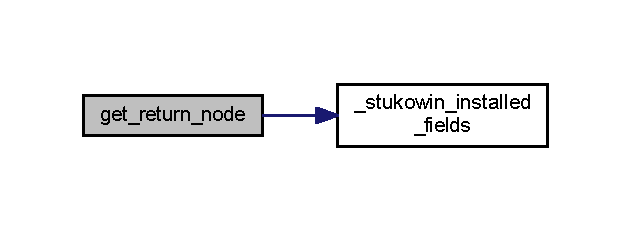
\includegraphics[width=303pt]{classcontent__manager_a6732db58443e8a0948bcc7705f654c7a_cgraph}
\end{center}
\end{figure}


\hypertarget{classcontent__manager_a3c6667e24648fecc0ec3751318ac55bd}{\index{content\+\_\+manager@{content\+\_\+manager}!get\+Curricula@{get\+Curricula}}
\index{get\+Curricula@{get\+Curricula}!content\+\_\+manager@{content\+\_\+manager}}
\paragraph[{get\+Curricula}]{\setlength{\rightskip}{0pt plus 5cm}get\+Curricula (
\begin{DoxyParamCaption}
\item[{}]{\$s\+Curr\+Type = {\ttfamily ''}, }
\item[{}]{\$a\+Vocabulary\+Types = {\ttfamily array('curriculum')}, }
\item[{}]{\$s\+Lang = {\ttfamily 'de'}}
\end{DoxyParamCaption}
)}}\label{classcontent__manager_a3c6667e24648fecc0ec3751318ac55bd}


Gets multiple curriculula. 

This method reads all curricula of curriculum type {\itshape \$s\+Curr\+Type} and vocabulary types {\itshape \$a\+Vocabulary\+Types} in the language {\itshape \$s\+Lang} from the drupal database and returns them as an associative array.


\begin{DoxyParams}[1]{Parameters}
string & {\em \$s\+Curr\+Type} & The type of curriculum to get. Valid values are
\begin{DoxyItemize}
\item Bachelorstudium
\item Masterstudium 
\end{DoxyItemize}\\
\hline
array & {\em \$a\+Vocabulary\+Types} & The taxonomy types to get. Default is 'curriculum'. Valid values are
\begin{DoxyItemize}
\item curriculum
\item itsv
\item schwerpunkt 
\end{DoxyItemize}\\
\hline
string & {\em \$s\+Lang} & The language to get the curricula in. Default is 'de' \\
\hline
\end{DoxyParams}
\begin{DoxyReturn}{Returns}
Associative array of selected curricula
\end{DoxyReturn}
\begin{DoxyAuthor}{Author}
Jakob Strasser -\/ \href{mailto:jakob.strasser@telenet.be}{\tt jakob.\+strasser@telenet.\+be} 
\end{DoxyAuthor}
\begin{DoxySince}{Since}
Commit \href{http://github.com/TheJake123/DrupalModul/commit/190577568295b7682dc74a79c4fd478e9e33c639}{\tt 1905775} on 2014-\/07-\/02 
\end{DoxySince}


Definition at line 189 of file content\+\_\+manager.\+inc.\+php.

\hypertarget{classcontent__manager_a0fccc30120c83ecc35b6a84b4654f2dc}{\index{content\+\_\+manager@{content\+\_\+manager}!get\+Curriculum@{get\+Curriculum}}
\index{get\+Curriculum@{get\+Curriculum}!content\+\_\+manager@{content\+\_\+manager}}
\paragraph[{get\+Curriculum}]{\setlength{\rightskip}{0pt plus 5cm}get\+Curriculum (
\begin{DoxyParamCaption}
\item[{}]{\$i\+V\+I\+D}
\end{DoxyParamCaption}
)}}\label{classcontent__manager_a0fccc30120c83ecc35b6a84b4654f2dc}


Gets one the curriculum. 

This function fetches the curriculum object with the given vocabulary id ({\itshape \$i\+V\+I\+D}) from the database.

{\bfseries Note\+:} it does not fetch the vocabulary tree, just its meta-\/information.


\begin{DoxyParams}[1]{Parameters}
integer & {\em \$i\+V\+I\+D} & The vid of the curriculum vocabulary \\
\hline
\end{DoxyParams}
\begin{DoxyReturn}{Returns}
An associative array representing the curriculum object
\end{DoxyReturn}
\begin{DoxyAuthor}{Author}
Jakob Strasser -\/ \href{mailto:jakob.strasser@telenet.be}{\tt jakob.\+strasser@telenet.\+be} 
\end{DoxyAuthor}
\begin{DoxySince}{Since}
Commit \href{http://github.com/TheJake123/DrupalModul/commit/190577568295b7682dc74a79c4fd478e9e33c639}{\tt 1905775} on 2014-\/07-\/02 
\end{DoxySince}


Definition at line 268 of file content\+\_\+manager.\+inc.\+php.

\hypertarget{classcontent__manager_a5d110b5c929715c771e2d903951ef7ca}{\index{content\+\_\+manager@{content\+\_\+manager}!get\+Unique\+Machine\+Name@{get\+Unique\+Machine\+Name}}
\index{get\+Unique\+Machine\+Name@{get\+Unique\+Machine\+Name}!content\+\_\+manager@{content\+\_\+manager}}
\paragraph[{get\+Unique\+Machine\+Name}]{\setlength{\rightskip}{0pt plus 5cm}get\+Unique\+Machine\+Name (
\begin{DoxyParamCaption}
\item[{}]{\$s\+Core\+Name}
\end{DoxyParamCaption}
)}}\label{classcontent__manager_a5d110b5c929715c771e2d903951ef7ca}


Gets a unique and valid machine name. 

This function asserts that a machine name is valid and adds incrementing numbers at the end until it is also unique.


\begin{DoxyParams}[1]{Parameters}
string & {\em \$s\+Core\+Name} & The initial name \\
\hline
\end{DoxyParams}
\begin{DoxyReturn}{Returns}
The unique and valid machine name
\end{DoxyReturn}
\begin{DoxyAuthor}{Author}
Jakob Strasser -\/ \href{mailto:jakob.strasser@telenet.be}{\tt jakob.\+strasser@telenet.\+be} 
\end{DoxyAuthor}
\begin{DoxySince}{Since}
Commit \href{http://github.com/TheJake123/DrupalModul/commit/190577568295b7682dc74a79c4fd478e9e33c639}{\tt 1905775} on 2014-\/07-\/02
\end{DoxySince}
\begin{DoxySeeAlso}{See also}
\hyperlink{group___drupal2_i_t_s_v_ga5fb85a53362f6fef40035a6c350c11ea}{stukowin\+\_\+taxonomy\+\_\+menu\+\_\+submit()} 

\hyperlink{classceus__importer_a5cd89fd2b1560b25eb4300ea6662a1b7}{ceus\+\_\+importer\+::check\+\_\+vocabulary()} 
\end{DoxySeeAlso}


Definition at line 230 of file content\+\_\+manager.\+inc.\+php.

\hypertarget{classcontent__manager_abe8407588c7195d203e7df5ff53fb373}{\index{content\+\_\+manager@{content\+\_\+manager}!json\+\_\+service\+\_\+curriculum@{json\+\_\+service\+\_\+curriculum}}
\index{json\+\_\+service\+\_\+curriculum@{json\+\_\+service\+\_\+curriculum}!content\+\_\+manager@{content\+\_\+manager}}
\paragraph[{json\+\_\+service\+\_\+curriculum}]{\setlength{\rightskip}{0pt plus 5cm}json\+\_\+service\+\_\+curriculum (
\begin{DoxyParamCaption}
\item[{}]{\$i\+V\+I\+D}
\end{DoxyParamCaption}
)}}\label{classcontent__manager_abe8407588c7195d203e7df5ff53fb373}


Returns curriculum tree as J\+S\+O\+N array. 

This method gets the entire tree of the curriculum with the vocabulary id {\ttfamily \$i\+V\+I\+D} and returns it as a J\+S\+O\+N array.


\begin{DoxyParams}[1]{Parameters}
integer & {\em \$i\+V\+I\+D} & Drupal vocabulary id of the desired curriculum\\
\hline
\end{DoxyParams}
\begin{DoxyAuthor}{Author}
Konstantinos Dafalias -\/ \href{mailto:kdafalias@gmail.com}{\tt kdafalias@gmail.\+com} 
\end{DoxyAuthor}
\begin{DoxySince}{Since}
Commit \href{http://github.com/TheJake123/DrupalModul/commit/f90560aa796b39853beb42a521d6d94c86051c46}{\tt f90560a} on 2014-\/06-\/28
\end{DoxySince}
\begin{DoxySeeAlso}{See also}
\hyperlink{classcontent__manager_acfeb4c387a22e750487e1bee5c73c1f9}{taxonomy\+\_\+get\+\_\+nested\+\_\+tree()} 
\end{DoxySeeAlso}


Definition at line 294 of file content\+\_\+manager.\+inc.\+php.

\hypertarget{classcontent__manager_a4f357170f7656cabf748245c46d7e8be}{\index{content\+\_\+manager@{content\+\_\+manager}!json\+\_\+service\+\_\+lva@{json\+\_\+service\+\_\+lva}}
\index{json\+\_\+service\+\_\+lva@{json\+\_\+service\+\_\+lva}!content\+\_\+manager@{content\+\_\+manager}}
\paragraph[{json\+\_\+service\+\_\+lva}]{\setlength{\rightskip}{0pt plus 5cm}json\+\_\+service\+\_\+lva (
\begin{DoxyParamCaption}
\item[{}]{\$i\+Node\+I\+D}
\end{DoxyParamCaption}
)}}\label{classcontent__manager_a4f357170f7656cabf748245c46d7e8be}


Returns course as J\+S\+O\+N object. 

This method fetches a single course from the drupal database and returns it as J\+S\+O\+N.


\begin{DoxyParams}[1]{Parameters}
integer & {\em \$i\+Node\+I\+D} & Content node id of the desired course\\
\hline
\end{DoxyParams}
\begin{DoxyAuthor}{Author}
Konstantinos Dafalias -\/ \href{mailto:kdafalias@gmail.com}{\tt kdafalias@gmail.\+com} 
\end{DoxyAuthor}
\begin{DoxySince}{Since}
Commit \href{http://github.com/TheJake123/DrupalModul/commit/f90560aa796b39853beb42a521d6d94c86051c46}{\tt f90560a} on 2014-\/06-\/28
\end{DoxySince}
\begin{DoxySeeAlso}{See also}
\hyperlink{group___drupal2_a_g_g_ga7522e206f1a87971b916a7a0be0098c6}{stukowin\+\_\+get\+\_\+lva()} 
\end{DoxySeeAlso}


Definition at line 155 of file content\+\_\+manager.\+inc.\+php.

\hypertarget{classcontent__manager_acfeb4c387a22e750487e1bee5c73c1f9}{\index{content\+\_\+manager@{content\+\_\+manager}!taxonomy\+\_\+get\+\_\+nested\+\_\+tree@{taxonomy\+\_\+get\+\_\+nested\+\_\+tree}}
\index{taxonomy\+\_\+get\+\_\+nested\+\_\+tree@{taxonomy\+\_\+get\+\_\+nested\+\_\+tree}!content\+\_\+manager@{content\+\_\+manager}}
\paragraph[{taxonomy\+\_\+get\+\_\+nested\+\_\+tree}]{\setlength{\rightskip}{0pt plus 5cm}taxonomy\+\_\+get\+\_\+nested\+\_\+tree (
\begin{DoxyParamCaption}
\item[{}]{\$vid\+\_\+or\+\_\+terms = {\ttfamily array()}, }
\item[{}]{\$max\+\_\+depth = {\ttfamily NULL}, }
\item[{}]{\$parent = {\ttfamily 0}, }
\item[{}]{\$parents\+\_\+index = {\ttfamily array()}, }
\item[{}]{\$depth = {\ttfamily 0}}
\end{DoxyParamCaption}
)}}\label{classcontent__manager_acfeb4c387a22e750487e1bee5c73c1f9}


Gets vocabulary tree. 

This is a recursive function that reads an entire drupal vocabulary into a nested array. It can be called externally by giving the vocabulary id (vid) as the first parameter and leaving the other parameters empty.


\begin{DoxyParams}[1]{Parameters}
integer | array & {\em \$vid\+\_\+or\+\_\+terms} & The vid of the curriculum to get. Default is an empty {\ttfamily array} \\
\hline
integer & {\em \$max\+\_\+depth} & The maximum depth of the nested array. Default is {\ttfamily N\+U\+L\+L} \\
\hline
integer & {\em \$parent} & The drupal term id (tid) of the next term's parent term. Default is {\ttfamily 0} \\
\hline
array & {\em \$parents\+\_\+index} & An array of all parents that have been traversed by the method in earlier recursion steps. Default is an empty {\ttfamily array} \\
\hline
integer & {\em \$depth} & The current recursion depth. Defaul is {\ttfamily 0} \\
\hline
\end{DoxyParams}
\begin{DoxyReturn}{Returns}
The nested array of all courses in the vocabulary
\end{DoxyReturn}
\begin{DoxyAuthor}{Author}
Konstantinos Dafalias -\/ \href{mailto:kdafalias@gmail.com}{\tt kdafalias@gmail.\+com} 
\end{DoxyAuthor}
\begin{DoxySince}{Since}
Commit \href{http://github.com/TheJake123/DrupalModul/commit/f90560aa796b39853beb42a521d6d94c86051c46}{\tt f90560a} on 2014-\/06-\/28 
\end{DoxySince}


Definition at line 106 of file content\+\_\+manager.\+inc.\+php.



References \+\_\+stukowin\+\_\+installed\+\_\+fields().



Here is the call graph for this function\+:
\nopagebreak
\begin{figure}[H]
\begin{center}
\leavevmode
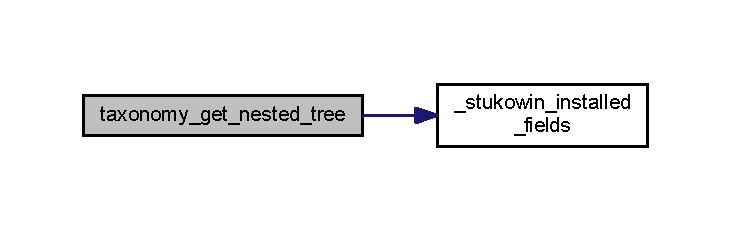
\includegraphics[width=350pt]{classcontent__manager_acfeb4c387a22e750487e1bee5c73c1f9_cgraph}
\end{center}
\end{figure}




The documentation for this class was generated from the following file\+:\begin{DoxyCompactItemize}
\item 
\hyperlink{content__manager_8inc_8php}{content\+\_\+manager.\+inc.\+php}\end{DoxyCompactItemize}

\hypertarget{union_e_x_s_t_y_p_e}{\subsection{E\+X\+S\+T\+Y\+P\+E Union Reference}
\label{union_e_x_s_t_y_p_e}\index{E\+X\+S\+T\+Y\+P\+E@{E\+X\+S\+T\+Y\+P\+E}}
}


{\ttfamily \#include $<$exparse.\+h$>$}

\subsubsection*{Data Fields}
\begin{DoxyCompactItemize}
\item 
struct Exnode\+\_\+s $\ast$ \hyperlink{union_e_x_s_t_y_p_e_a5147a7084c9f4929f621b9c1d88f37e4}{expr}
\item 
double \hyperlink{union_e_x_s_t_y_p_e_a347120387fb1d297ddcdf38a1fe7578f}{floating}
\item 
struct Exref\+\_\+s $\ast$ \hyperlink{union_e_x_s_t_y_p_e_a978c478f22a8ae8e29c509cbba1426e4}{reference}
\item 
struct Exid\+\_\+s $\ast$ \hyperlink{union_e_x_s_t_y_p_e_a8cbcc48b98839e0560a1b4ea77ad9fce}{id}
\item 
Sflong\+\_\+t \hyperlink{union_e_x_s_t_y_p_e_a18927fffeef0d58b4627da1446d7b0b8}{integer}
\item 
int \hyperlink{union_e_x_s_t_y_p_e_a8b21910e53867f3b53d61a8c46ac2a7f}{op}
\item 
char $\ast$ \hyperlink{union_e_x_s_t_y_p_e_aed1cfb225a5fb77461e7972691e68a72}{string}
\item 
void $\ast$ \hyperlink{union_e_x_s_t_y_p_e_a5ab32084b1ccaf8aaa8a0c703b8853cf}{user}
\item 
struct Exbuf\+\_\+s $\ast$ \hyperlink{union_e_x_s_t_y_p_e_acfa12300629fea2a3f9e9651b7baaa97}{buffer}
\end{DoxyCompactItemize}


\subsubsection{Detailed Description}


Definition at line 208 of file exparse.\+h.



\subsubsection{Field Documentation}
\hypertarget{union_e_x_s_t_y_p_e_acfa12300629fea2a3f9e9651b7baaa97}{\index{E\+X\+S\+T\+Y\+P\+E@{E\+X\+S\+T\+Y\+P\+E}!buffer@{buffer}}
\index{buffer@{buffer}!E\+X\+S\+T\+Y\+P\+E@{E\+X\+S\+T\+Y\+P\+E}}
\paragraph[{buffer}]{\setlength{\rightskip}{0pt plus 5cm}struct Exbuf\+\_\+s$\ast$ buffer}}\label{union_e_x_s_t_y_p_e_acfa12300629fea2a3f9e9651b7baaa97}


Definition at line 222 of file exparse.\+h.

\hypertarget{union_e_x_s_t_y_p_e_a5147a7084c9f4929f621b9c1d88f37e4}{\index{E\+X\+S\+T\+Y\+P\+E@{E\+X\+S\+T\+Y\+P\+E}!expr@{expr}}
\index{expr@{expr}!E\+X\+S\+T\+Y\+P\+E@{E\+X\+S\+T\+Y\+P\+E}}
\paragraph[{expr}]{\setlength{\rightskip}{0pt plus 5cm}struct Exnode\+\_\+s$\ast$ expr}}\label{union_e_x_s_t_y_p_e_a5147a7084c9f4929f621b9c1d88f37e4}


Definition at line 214 of file exparse.\+h.

\hypertarget{union_e_x_s_t_y_p_e_a347120387fb1d297ddcdf38a1fe7578f}{\index{E\+X\+S\+T\+Y\+P\+E@{E\+X\+S\+T\+Y\+P\+E}!floating@{floating}}
\index{floating@{floating}!E\+X\+S\+T\+Y\+P\+E@{E\+X\+S\+T\+Y\+P\+E}}
\paragraph[{floating}]{\setlength{\rightskip}{0pt plus 5cm}double floating}}\label{union_e_x_s_t_y_p_e_a347120387fb1d297ddcdf38a1fe7578f}


Definition at line 215 of file exparse.\+h.

\hypertarget{union_e_x_s_t_y_p_e_a8cbcc48b98839e0560a1b4ea77ad9fce}{\index{E\+X\+S\+T\+Y\+P\+E@{E\+X\+S\+T\+Y\+P\+E}!id@{id}}
\index{id@{id}!E\+X\+S\+T\+Y\+P\+E@{E\+X\+S\+T\+Y\+P\+E}}
\paragraph[{id}]{\setlength{\rightskip}{0pt plus 5cm}struct Exid\+\_\+s$\ast$ id}}\label{union_e_x_s_t_y_p_e_a8cbcc48b98839e0560a1b4ea77ad9fce}


Definition at line 217 of file exparse.\+h.

\hypertarget{union_e_x_s_t_y_p_e_a18927fffeef0d58b4627da1446d7b0b8}{\index{E\+X\+S\+T\+Y\+P\+E@{E\+X\+S\+T\+Y\+P\+E}!integer@{integer}}
\index{integer@{integer}!E\+X\+S\+T\+Y\+P\+E@{E\+X\+S\+T\+Y\+P\+E}}
\paragraph[{integer}]{\setlength{\rightskip}{0pt plus 5cm}Sflong\+\_\+t integer}}\label{union_e_x_s_t_y_p_e_a18927fffeef0d58b4627da1446d7b0b8}


Definition at line 218 of file exparse.\+h.

\hypertarget{union_e_x_s_t_y_p_e_a8b21910e53867f3b53d61a8c46ac2a7f}{\index{E\+X\+S\+T\+Y\+P\+E@{E\+X\+S\+T\+Y\+P\+E}!op@{op}}
\index{op@{op}!E\+X\+S\+T\+Y\+P\+E@{E\+X\+S\+T\+Y\+P\+E}}
\paragraph[{op}]{\setlength{\rightskip}{0pt plus 5cm}int op}}\label{union_e_x_s_t_y_p_e_a8b21910e53867f3b53d61a8c46ac2a7f}


Definition at line 219 of file exparse.\+h.

\hypertarget{union_e_x_s_t_y_p_e_a978c478f22a8ae8e29c509cbba1426e4}{\index{E\+X\+S\+T\+Y\+P\+E@{E\+X\+S\+T\+Y\+P\+E}!reference@{reference}}
\index{reference@{reference}!E\+X\+S\+T\+Y\+P\+E@{E\+X\+S\+T\+Y\+P\+E}}
\paragraph[{reference}]{\setlength{\rightskip}{0pt plus 5cm}struct Exref\+\_\+s$\ast$ reference}}\label{union_e_x_s_t_y_p_e_a978c478f22a8ae8e29c509cbba1426e4}


Definition at line 216 of file exparse.\+h.

\hypertarget{union_e_x_s_t_y_p_e_aed1cfb225a5fb77461e7972691e68a72}{\index{E\+X\+S\+T\+Y\+P\+E@{E\+X\+S\+T\+Y\+P\+E}!string@{string}}
\index{string@{string}!E\+X\+S\+T\+Y\+P\+E@{E\+X\+S\+T\+Y\+P\+E}}
\paragraph[{string}]{\setlength{\rightskip}{0pt plus 5cm}char$\ast$ string}}\label{union_e_x_s_t_y_p_e_aed1cfb225a5fb77461e7972691e68a72}


Definition at line 220 of file exparse.\+h.

\hypertarget{union_e_x_s_t_y_p_e_a5ab32084b1ccaf8aaa8a0c703b8853cf}{\index{E\+X\+S\+T\+Y\+P\+E@{E\+X\+S\+T\+Y\+P\+E}!user@{user}}
\index{user@{user}!E\+X\+S\+T\+Y\+P\+E@{E\+X\+S\+T\+Y\+P\+E}}
\paragraph[{user}]{\setlength{\rightskip}{0pt plus 5cm}void$\ast$ user}}\label{union_e_x_s_t_y_p_e_a5ab32084b1ccaf8aaa8a0c703b8853cf}


Definition at line 221 of file exparse.\+h.



The documentation for this union was generated from the following file\+:\begin{DoxyCompactItemize}
\item 
\hyperlink{exparse_8h}{exparse.\+h}\end{DoxyCompactItemize}

\hypertarget{classoverview_p_d_f}{\subsection{overview\+P\+D\+F Class Reference}
\label{classoverview_p_d_f}\index{overview\+P\+D\+F@{overview\+P\+D\+F}}
}


Class for P\+D\+F document generation from curricula data.  




Inheritance diagram for overview\+P\+D\+F\+:
\nopagebreak
\begin{figure}[H]
\begin{center}
\leavevmode
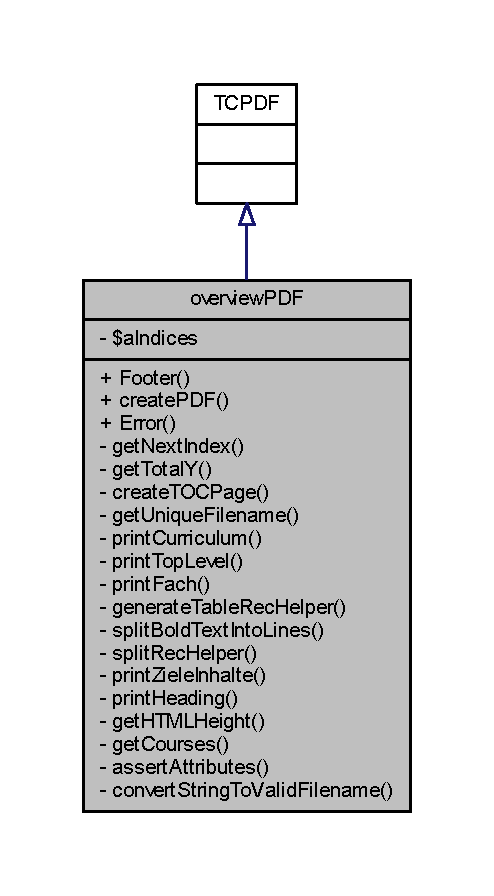
\includegraphics[width=237pt]{classoverview_p_d_f__inherit__graph}
\end{center}
\end{figure}
\subsubsection*{Public Member Functions}
\begin{DoxyCompactItemize}
\item 
\hyperlink{classoverview_p_d_f_a2f39533ba0786237090683635ef01c49}{Footer} ()
\begin{DoxyCompactList}\small\item\em Generates Footer for each page. \end{DoxyCompactList}\item 
\hyperlink{classoverview_p_d_f_a30ddd92aaf87bca0825c149bd3a7d43f}{create\+P\+D\+F} (\$i\+V\+I\+D)
\begin{DoxyCompactList}\small\item\em Creates the P\+D\+F document. \end{DoxyCompactList}\item 
\hyperlink{classoverview_p_d_f_a5afab85a7aaf19395f9a0e86cae76928}{Error} (\$msg)
\begin{DoxyCompactList}\small\item\em Throws exception in case of an error. \end{DoxyCompactList}\end{DoxyCompactItemize}
\subsubsection*{Private Member Functions}
\begin{DoxyCompactItemize}
\item 
\hyperlink{classoverview_p_d_f_aedc9466cae51e07e57ba865a69c92efc}{get\+Next\+Index} (\$i\+Level)
\begin{DoxyCompactList}\small\item\em Gets index of the desired level. \end{DoxyCompactList}\item 
\hyperlink{classoverview_p_d_f_adca20f06977ea2b3b8737b1d465a1606}{get\+Total\+Y} ()
\begin{DoxyCompactList}\small\item\em Gets the full y-\/position in the document. \end{DoxyCompactList}\item 
\hyperlink{classoverview_p_d_f_acf4bdf38a6e11c036b076a16c3516f75}{create\+T\+O\+C\+Page} ()
\begin{DoxyCompactList}\small\item\em Adds a table of contents page to the P\+D\+F document. \end{DoxyCompactList}\item 
\hyperlink{classoverview_p_d_f_a10c644f1f84ae1b261a8b198a66b5cb1}{get\+Unique\+Filename} (\$s\+Curr\+Type, \$s\+Curr\+Version)
\begin{DoxyCompactList}\small\item\em Creates a unique filename. \end{DoxyCompactList}\item 
\hyperlink{classoverview_p_d_f_a1871e6880b3bb67d0a49cdcab4cd680d}{print\+Curriculum} (\$o\+Curriculum)
\begin{DoxyCompactList}\small\item\em Prints a curriculum object and all its courses to the P\+D\+F document. \end{DoxyCompactList}\item 
\hyperlink{classoverview_p_d_f_a23c7451efb8c436590fbad032bc6788b}{print\+Top\+Level} (\$o\+Top\+Level)
\begin{DoxyCompactList}\small\item\em Decides whether to print a structural element or a subject. \end{DoxyCompactList}\item 
\hyperlink{classoverview_p_d_f_abf0674d88080affc25c472fbd0525896}{print\+Fach} (\$o\+Fach)
\begin{DoxyCompactList}\small\item\em Prints a subject to the P\+D\+F document. \end{DoxyCompactList}\item 
\hyperlink{classoverview_p_d_f_ad0ea6c6476d690b08161300e40926dc6}{generate\+Table\+Rec\+Helper} (\$o\+Course)
\begin{DoxyCompactList}\small\item\em Recursive function for generating overview table. \end{DoxyCompactList}\item 
\hyperlink{classoverview_p_d_f_aa12feabadc0d4aa85bb4da7454f8245d}{split\+Bold\+Text\+Into\+Lines} (\$s\+Text, \$i\+Max\+Width)
\begin{DoxyCompactList}\small\item\em Inserts line breaks into bold text. \end{DoxyCompactList}\item 
\hyperlink{classoverview_p_d_f_af3f9a49de14251ba45bd046879f27aa2}{split\+Rec\+Helper} (\$a\+Words, \$i\+Curr\+Index, \$i\+Max\+Width)
\begin{DoxyCompactList}\small\item\em Recursive helper function for \hyperlink{classoverview_p_d_f_aa12feabadc0d4aa85bb4da7454f8245d}{split\+Bold\+Text\+Into\+Lines()} \end{DoxyCompactList}\item 
\hyperlink{classoverview_p_d_f_af0b14d64b47fe81df7965b8259ccb762}{print\+Ziele\+Inhalte} (\$o\+Course)
\begin{DoxyCompactList}\small\item\em Prints the course goals and content of teaching and their respecitve headings to the document. \end{DoxyCompactList}\item 
\hyperlink{classoverview_p_d_f_ad6b57d30526fb658521faddce7595dc4}{print\+Heading} (\$s\+Text, \$i\+Level, \$b\+Show\+Index=true, \$s\+Align= 'L', \$b\+Add\+Bookmark=true)
\begin{DoxyCompactList}\small\item\em Prints a heading to the P\+D\+F document. \end{DoxyCompactList}\end{DoxyCompactItemize}
\subsubsection*{Static Private Member Functions}
\begin{DoxyCompactItemize}
\item 
static \hyperlink{classoverview_p_d_f_af41675b946292789cecd9416ca809bcc}{get\+H\+T\+M\+L\+Height} (\$s\+H\+T\+M\+L)
\begin{DoxyCompactList}\small\item\em Determines height of H\+T\+M\+L Code. \end{DoxyCompactList}\item 
static \hyperlink{classoverview_p_d_f_a921bc685431e16db85dc8ef8491f90a4}{get\+Courses} (\$curr\+Id)
\begin{DoxyCompactList}\small\item\em Gets all courses for a given curriculum id. \end{DoxyCompactList}\item 
static \hyperlink{classoverview_p_d_f_a56f3ef341ae39bb7b4c34a700b33eac1}{assert\+Attributes} (\$o\+Course)
\begin{DoxyCompactList}\small\item\em Guarantees the existence of the specified attributes in the course and all its children. \end{DoxyCompactList}\item 
static \hyperlink{classoverview_p_d_f_ab867930d00ec2effc61f252de44b04fe}{convert\+String\+To\+Valid\+Filename} (\$s\+String)
\begin{DoxyCompactList}\small\item\em Utility method that formats a string into a valid file name. \end{DoxyCompactList}\end{DoxyCompactItemize}
\subsubsection*{Private Attributes}
\begin{DoxyCompactItemize}
\item 
\hyperlink{classoverview_p_d_f_a7d055132da646af2b192923c6a864e97}{\$a\+Indices} = array ()
\begin{DoxyCompactList}\small\item\em Array of indices for continuous indexation of headings. \end{DoxyCompactList}\end{DoxyCompactItemize}


\subsubsection{Detailed Description}
Class for P\+D\+F document generation from curricula data. 

This class provides the functionality for automatically generating a P\+D\+F document from a curriculum.

It is publicly accessible through the \hyperlink{classoverview_p_d_f_a30ddd92aaf87bca0825c149bd3a7d43f}{create\+P\+D\+F()} method, which initiates and guides the P\+D\+F generation.

\begin{DoxyAuthor}{Author}
Jakob Strasser -\/ \href{mailto:jakob.strasser@telenet.be}{\tt jakob.\+strasser@telenet.\+be} 
\end{DoxyAuthor}
\begin{DoxyAuthor}{Authors}
Fabian Puehringer -\/ \href{mailto:f.puehringer@24speed.at}{\tt f.\+puehringer@24speed.\+at} 
\end{DoxyAuthor}
\begin{DoxyVersion}{Version}
1.\+0.\+3 2014-\/07-\/22 
\end{DoxyVersion}
\begin{DoxySince}{Since}
Commit \href{http://github.com/TheJake123/DrupalModul/commit/b9342d941b3f93e212f3f6af0823a07524dd5954}{\tt b9342d9} on 2014-\/06-\/30
\end{DoxySince}
\begin{DoxySeeAlso}{See also}
\hyperlink{classoverview_p_d_f_a30ddd92aaf87bca0825c149bd3a7d43f}{create\+P\+D\+F()} 
\end{DoxySeeAlso}


Definition at line 62 of file pdf\+\_\+creator.\+inc.\+php.



\subsubsection{Member Function Documentation}
\hypertarget{classoverview_p_d_f_a56f3ef341ae39bb7b4c34a700b33eac1}{\index{overview\+P\+D\+F@{overview\+P\+D\+F}!assert\+Attributes@{assert\+Attributes}}
\index{assert\+Attributes@{assert\+Attributes}!overview\+P\+D\+F@{overview\+P\+D\+F}}
\paragraph[{assert\+Attributes}]{\setlength{\rightskip}{0pt plus 5cm}static assert\+Attributes (
\begin{DoxyParamCaption}
\item[{}]{\$o\+Course}
\end{DoxyParamCaption}
)\hspace{0.3cm}{\ttfamily [static]}, {\ttfamily [private]}}}\label{classoverview_p_d_f_a56f3ef341ae39bb7b4c34a700b33eac1}


Guarantees the existence of the specified attributes in the course and all its children. 

This is a recursive helper method which asserts that the following attributes exist in the course object\+:
\begin{DoxyItemize}
\item title
\item ects
\item wst
\item lvatype
\item typename
\item ziele
\item lehrinhalte
\item lvtypshort
\item typename
\end{DoxyItemize}

Needed so that the other methods do not have to check everytime an attribute is accessed.


\begin{DoxyParams}[1]{Parameters}
object & {\em \$o\+Course} & The course to assert the attributes for\\
\hline
\end{DoxyParams}
\begin{DoxyAuthor}{Author}
Jakob Strasser -\/ \href{mailto:jakob.strasser@telenet.be}{\tt jakob.\+strasser@telenet.\+be} 
\end{DoxyAuthor}
\begin{DoxySince}{Since}
Commit \href{http://github.com/TheJake123/DrupalModul/commit/b9342d941b3f93e212f3f6af0823a07524dd5954}{\tt b9342d9} on 2014-\/06-\/30 
\end{DoxySince}


Definition at line 638 of file pdf\+\_\+creator.\+inc.\+php.



Referenced by get\+Courses().



Here is the caller graph for this function\+:
\nopagebreak
\begin{figure}[H]
\begin{center}
\leavevmode
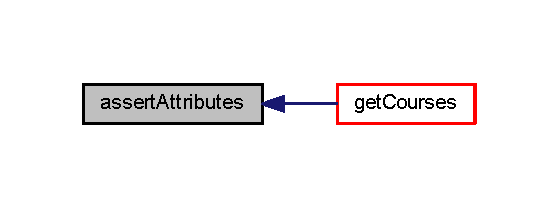
\includegraphics[width=268pt]{classoverview_p_d_f_a56f3ef341ae39bb7b4c34a700b33eac1_icgraph}
\end{center}
\end{figure}


\hypertarget{classoverview_p_d_f_ab867930d00ec2effc61f252de44b04fe}{\index{overview\+P\+D\+F@{overview\+P\+D\+F}!convert\+String\+To\+Valid\+Filename@{convert\+String\+To\+Valid\+Filename}}
\index{convert\+String\+To\+Valid\+Filename@{convert\+String\+To\+Valid\+Filename}!overview\+P\+D\+F@{overview\+P\+D\+F}}
\paragraph[{convert\+String\+To\+Valid\+Filename}]{\setlength{\rightskip}{0pt plus 5cm}static convert\+String\+To\+Valid\+Filename (
\begin{DoxyParamCaption}
\item[{}]{\$s\+String}
\end{DoxyParamCaption}
)\hspace{0.3cm}{\ttfamily [static]}, {\ttfamily [private]}}}\label{classoverview_p_d_f_ab867930d00ec2effc61f252de44b04fe}


Utility method that formats a string into a valid file name. 


\begin{DoxyParams}[1]{Parameters}
string & {\em \$s\+String} & The file name to validate \\
\hline
\end{DoxyParams}
\begin{DoxyReturn}{Returns}
The valid file name created from the input
\end{DoxyReturn}
\begin{DoxyAuthor}{Author}
Konstantinos Dafalias -\/ \href{mailto:kdafalias@gmail.com}{\tt kdafalias@gmail.\+com} 
\end{DoxyAuthor}
\begin{DoxySince}{Since}
Commit \href{http://github.com/TheJake123/DrupalModul/commit/f157d51285e8cc638db4a8f62c7635e5ed2bb2fd}{\tt f157d51} on 2014-\/07-\/06 
\end{DoxySince}


Definition at line 672 of file pdf\+\_\+creator.\+inc.\+php.



Referenced by get\+Unique\+Filename().



Here is the caller graph for this function\+:
\nopagebreak
\begin{figure}[H]
\begin{center}
\leavevmode
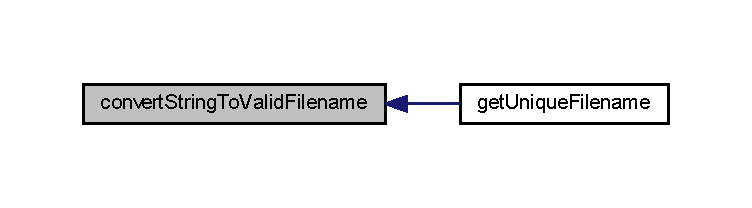
\includegraphics[width=350pt]{classoverview_p_d_f_ab867930d00ec2effc61f252de44b04fe_icgraph}
\end{center}
\end{figure}


\hypertarget{classoverview_p_d_f_a30ddd92aaf87bca0825c149bd3a7d43f}{\index{overview\+P\+D\+F@{overview\+P\+D\+F}!create\+P\+D\+F@{create\+P\+D\+F}}
\index{create\+P\+D\+F@{create\+P\+D\+F}!overview\+P\+D\+F@{overview\+P\+D\+F}}
\paragraph[{create\+P\+D\+F}]{\setlength{\rightskip}{0pt plus 5cm}create\+P\+D\+F (
\begin{DoxyParamCaption}
\item[{}]{\$i\+V\+I\+D}
\end{DoxyParamCaption}
)}}\label{classoverview_p_d_f_a30ddd92aaf87bca0825c149bd3a7d43f}


Creates the P\+D\+F document. 

This method is the main public method of the \hyperlink{classoverview_p_d_f}{overview\+P\+D\+F} class. It manages the entire document generation and saves the P\+D\+F to the preconfigured path. The steps for creating the document are as follows\+:
\begin{DoxyEnumerate}
\item Set up P\+D\+F document
\item Set document meta information
\item Set up title page
\item Initiate printing of individual subjects
\item Add index page
\item Save the document
\end{DoxyEnumerate}


\begin{DoxyParams}[1]{Parameters}
integer & {\em \$i\+V\+I\+D} & Drupal vocabulary id of the desired Curriculum \\
\hline
\end{DoxyParams}
\begin{DoxyReturn}{Returns}
Success message\+: 'P\+D\+F successfully created at ' and the filepath
\end{DoxyReturn}
\begin{DoxyAuthor}{Author}
Jakob Strasser -\/ \href{mailto:jakob.strasser@telenet.be}{\tt jakob.\+strasser@telenet.\+be} 
\end{DoxyAuthor}
\begin{DoxySince}{Since}
Commit \href{http://github.com/TheJake123/DrupalModul/commit/b9342d941b3f93e212f3f6af0823a07524dd5954}{\tt b9342d9} on 2014-\/06-\/30
\end{DoxySince}
\begin{DoxySeeAlso}{See also}
\hyperlink{group___drupal2_p_d_f_ga3649714a54a489d8c0096116fd9cb367}{stukowin\+\_\+pdf\+\_\+menu()} 

\hyperlink{group___drupal2_p_d_f_ga7fd34094c899b5a82949f401e30139a1}{stukowin\+\_\+pdf\+\_\+menu\+\_\+submit()} 
\end{DoxySeeAlso}


Definition at line 195 of file pdf\+\_\+creator.\+inc.\+php.



References create\+T\+O\+C\+Page(), and print\+Curriculum().



Here is the call graph for this function\+:
\nopagebreak
\begin{figure}[H]
\begin{center}
\leavevmode
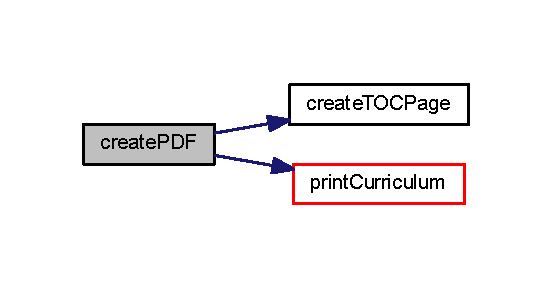
\includegraphics[width=265pt]{classoverview_p_d_f_a30ddd92aaf87bca0825c149bd3a7d43f_cgraph}
\end{center}
\end{figure}


\hypertarget{classoverview_p_d_f_acf4bdf38a6e11c036b076a16c3516f75}{\index{overview\+P\+D\+F@{overview\+P\+D\+F}!create\+T\+O\+C\+Page@{create\+T\+O\+C\+Page}}
\index{create\+T\+O\+C\+Page@{create\+T\+O\+C\+Page}!overview\+P\+D\+F@{overview\+P\+D\+F}}
\paragraph[{create\+T\+O\+C\+Page}]{\setlength{\rightskip}{0pt plus 5cm}create\+T\+O\+C\+Page (
\begin{DoxyParamCaption}
{}
\end{DoxyParamCaption}
)\hspace{0.3cm}{\ttfamily [private]}}}\label{classoverview_p_d_f_acf4bdf38a6e11c036b076a16c3516f75}


Adds a table of contents page to the P\+D\+F document. 

This method is called at the end of the document creation, after all subjects have been printed to the document, and inserts a table of contents (index) page as the second page in the document.

\begin{DoxyAuthor}{Author}
Jakob Strasser -\/ \href{mailto:jakob.strasser@telenet.be}{\tt jakob.\+strasser@telenet.\+be} 
\end{DoxyAuthor}
\begin{DoxySince}{Since}
Commit \href{http://github.com/TheJake123/DrupalModul/commit/b9342d941b3f93e212f3f6af0823a07524dd5954}{\tt b9342d9} on 2014-\/06-\/30
\end{DoxySince}
\begin{DoxySeeAlso}{See also}
T\+C\+P\+D\+F\+::add\+T\+O\+C\+Page() 

\hyperlink{classoverview_p_d_f_ad6b57d30526fb658521faddce7595dc4}{print\+Heading()} 
\end{DoxySeeAlso}


Definition at line 262 of file pdf\+\_\+creator.\+inc.\+php.



Referenced by create\+P\+D\+F().



Here is the caller graph for this function\+:
\nopagebreak
\begin{figure}[H]
\begin{center}
\leavevmode
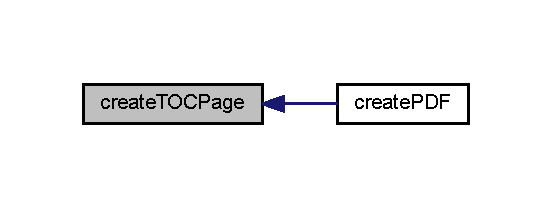
\includegraphics[width=265pt]{classoverview_p_d_f_acf4bdf38a6e11c036b076a16c3516f75_icgraph}
\end{center}
\end{figure}


\hypertarget{classoverview_p_d_f_a5afab85a7aaf19395f9a0e86cae76928}{\index{overview\+P\+D\+F@{overview\+P\+D\+F}!Error@{Error}}
\index{Error@{Error}!overview\+P\+D\+F@{overview\+P\+D\+F}}
\paragraph[{Error}]{\setlength{\rightskip}{0pt plus 5cm}Error (
\begin{DoxyParamCaption}
\item[{}]{\$msg}
\end{DoxyParamCaption}
)}}\label{classoverview_p_d_f_a5afab85a7aaf19395f9a0e86cae76928}


Throws exception in case of an error. 

This method is needed for displaying errors as drupal messages, due to \hyperlink{class_t_c_p_d_f}{T\+C\+P\+D\+F} normally displaying errors by itself and the dying.


\begin{DoxyParams}[1]{Parameters}
string & {\em \$msg} & The error message to throw the ecxeption with \\
\hline
\end{DoxyParams}

\begin{DoxyExceptions}{Exceptions}
{\em Exception} & A new exception with the given message\\
\hline
\end{DoxyExceptions}
\begin{DoxyAuthor}{Author}
Jakob Strasser -\/ \href{mailto:jakob.strasser@telenet.be}{\tt jakob.\+strasser@telenet.\+be} 
\end{DoxyAuthor}
\begin{DoxySince}{Since}
Commit \href{http://github.com/TheJake123/DrupalModul/commit/e4fa523cc03bdc9453581c7a43d23a09d4ee5688}{\tt e4fa523} on 2014-\/07-\/02
\end{DoxySince}
\begin{DoxySeeAlso}{See also}
T\+C\+P\+D\+F\+::\+Error() 
\end{DoxySeeAlso}


Definition at line 245 of file pdf\+\_\+creator.\+inc.\+php.

\hypertarget{classoverview_p_d_f_a2f39533ba0786237090683635ef01c49}{\index{overview\+P\+D\+F@{overview\+P\+D\+F}!Footer@{Footer}}
\index{Footer@{Footer}!overview\+P\+D\+F@{overview\+P\+D\+F}}
\paragraph[{Footer}]{\setlength{\rightskip}{0pt plus 5cm}Footer (
\begin{DoxyParamCaption}
{}
\end{DoxyParamCaption}
)}}\label{classoverview_p_d_f_a2f39533ba0786237090683635ef01c49}


Generates Footer for each page. 

This method draws a 1px line across the entire page 15mm above the bottom and writes the page number in the format \char`\"{}current page/total pages\char`\"{} into the bottom right corner.

\begin{DoxyAuthor}{Author}
Jakob Strasser -\/ \href{mailto:jakob.strasser@telenet.be}{\tt jakob.\+strasser@telenet.\+be} 
\end{DoxyAuthor}
\begin{DoxySince}{Since}
Commit \href{http://github.com/TheJake123/DrupalModul/commit/b9342d941b3f93e212f3f6af0823a07524dd5954}{\tt b9342d9} on 2014-\/06-\/30
\end{DoxySince}
\begin{DoxySeeAlso}{See also}
T\+C\+P\+D\+F\+::\+Footer() 
\end{DoxySeeAlso}


Definition at line 86 of file pdf\+\_\+creator.\+inc.\+php.

\hypertarget{classoverview_p_d_f_ad0ea6c6476d690b08161300e40926dc6}{\index{overview\+P\+D\+F@{overview\+P\+D\+F}!generate\+Table\+Rec\+Helper@{generate\+Table\+Rec\+Helper}}
\index{generate\+Table\+Rec\+Helper@{generate\+Table\+Rec\+Helper}!overview\+P\+D\+F@{overview\+P\+D\+F}}
\paragraph[{generate\+Table\+Rec\+Helper}]{\setlength{\rightskip}{0pt plus 5cm}generate\+Table\+Rec\+Helper (
\begin{DoxyParamCaption}
\item[{}]{\$o\+Course}
\end{DoxyParamCaption}
)\hspace{0.3cm}{\ttfamily [private]}}}\label{classoverview_p_d_f_ad0ea6c6476d690b08161300e40926dc6}


Recursive function for generating overview table. 

This is a recursive helper function for generating a subject overview table. It traverses the nested array of courses down to the leaves and creates a table row for each course.
\begin{DoxyItemize}
\item Subjects are printed in bold
\item Modules are printed in italics
\item Courses are printed in normal text
\end{DoxyItemize}


\begin{DoxyParams}[1]{Parameters}
object & {\em \$o\+Course} & The course to generate the table H\+T\+M\+L code for \\
\hline
\end{DoxyParams}
\begin{DoxyReturn}{Returns}
The H\+T\+M\+L code of the table rows for this course and all its children
\end{DoxyReturn}
\begin{DoxyAuthor}{Author}
Jakob Strasser -\/ \href{mailto:jakob.strasser@telenet.be}{\tt jakob.\+strasser@telenet.\+be} 
\end{DoxyAuthor}
\begin{DoxySince}{Since}
Commit \href{http://github.com/TheJake123/DrupalModul/commit/b9342d941b3f93e212f3f6af0823a07524dd5954}{\tt b9342d9} on 2014-\/06-\/30
\end{DoxySince}
\begin{DoxySeeAlso}{See also}
\hyperlink{classoverview_p_d_f_abf0674d88080affc25c472fbd0525896}{print\+Fach()} 
\end{DoxySeeAlso}


Definition at line 454 of file pdf\+\_\+creator.\+inc.\+php.



References split\+Bold\+Text\+Into\+Lines().



Referenced by print\+Fach().



Here is the call graph for this function\+:
\nopagebreak
\begin{figure}[H]
\begin{center}
\leavevmode
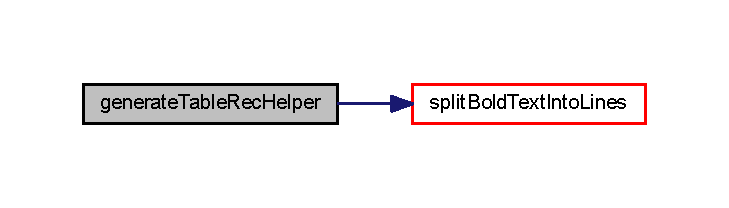
\includegraphics[width=350pt]{classoverview_p_d_f_ad0ea6c6476d690b08161300e40926dc6_cgraph}
\end{center}
\end{figure}




Here is the caller graph for this function\+:
\nopagebreak
\begin{figure}[H]
\begin{center}
\leavevmode
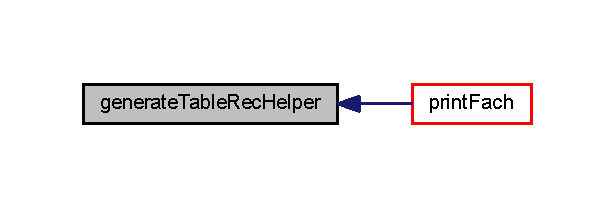
\includegraphics[width=295pt]{classoverview_p_d_f_ad0ea6c6476d690b08161300e40926dc6_icgraph}
\end{center}
\end{figure}


\hypertarget{classoverview_p_d_f_a921bc685431e16db85dc8ef8491f90a4}{\index{overview\+P\+D\+F@{overview\+P\+D\+F}!get\+Courses@{get\+Courses}}
\index{get\+Courses@{get\+Courses}!overview\+P\+D\+F@{overview\+P\+D\+F}}
\paragraph[{get\+Courses}]{\setlength{\rightskip}{0pt plus 5cm}static get\+Courses (
\begin{DoxyParamCaption}
\item[{}]{\$curr\+Id}
\end{DoxyParamCaption}
)\hspace{0.3cm}{\ttfamily [static]}, {\ttfamily [private]}}}\label{classoverview_p_d_f_a921bc685431e16db85dc8ef8491f90a4}


Gets all courses for a given curriculum id. 

This method gets all the courses in a curriculum and prepares them for further processing in the P\+D\+F creation process.


\begin{DoxyParams}[1]{Parameters}
integer & {\em \$curr\+Id} & The vocabulary id of the curriculum to get the courses from \\
\hline
\end{DoxyParams}
\begin{DoxyReturn}{Returns}
The nested array of all courses in the given curriculum
\end{DoxyReturn}
\begin{DoxyAuthor}{Author}
Jakob Strasser -\/ \href{mailto:jakob.strasser@telenet.be}{\tt jakob.\+strasser@telenet.\+be} 
\end{DoxyAuthor}
\begin{DoxySince}{Since}
Commit \href{http://github.com/TheJake123/DrupalModul/commit/b9342d941b3f93e212f3f6af0823a07524dd5954}{\tt b9342d9} on 2014-\/06-\/30 
\end{DoxySince}


Definition at line 608 of file pdf\+\_\+creator.\+inc.\+php.



References assert\+Attributes().



Referenced by print\+Curriculum().



Here is the call graph for this function\+:
\nopagebreak
\begin{figure}[H]
\begin{center}
\leavevmode
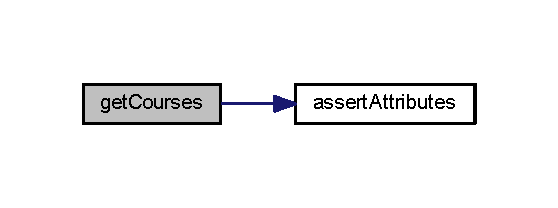
\includegraphics[width=268pt]{classoverview_p_d_f_a921bc685431e16db85dc8ef8491f90a4_cgraph}
\end{center}
\end{figure}




Here is the caller graph for this function\+:
\nopagebreak
\begin{figure}[H]
\begin{center}
\leavevmode
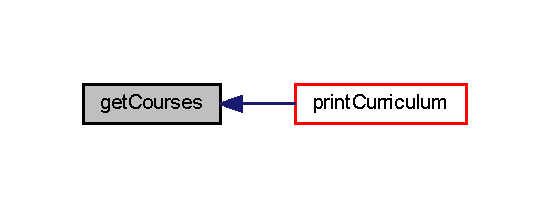
\includegraphics[width=264pt]{classoverview_p_d_f_a921bc685431e16db85dc8ef8491f90a4_icgraph}
\end{center}
\end{figure}


\hypertarget{classoverview_p_d_f_af41675b946292789cecd9416ca809bcc}{\index{overview\+P\+D\+F@{overview\+P\+D\+F}!get\+H\+T\+M\+L\+Height@{get\+H\+T\+M\+L\+Height}}
\index{get\+H\+T\+M\+L\+Height@{get\+H\+T\+M\+L\+Height}!overview\+P\+D\+F@{overview\+P\+D\+F}}
\paragraph[{get\+H\+T\+M\+L\+Height}]{\setlength{\rightskip}{0pt plus 5cm}static get\+H\+T\+M\+L\+Height (
\begin{DoxyParamCaption}
\item[{}]{\$s\+H\+T\+M\+L}
\end{DoxyParamCaption}
)\hspace{0.3cm}{\ttfamily [static]}, {\ttfamily [private]}}}\label{classoverview_p_d_f_af41675b946292789cecd9416ca809bcc}


Determines height of H\+T\+M\+L Code. 

This utility method prints {\itshape \$s\+H\+T\+M\+L} to a test instance of \hyperlink{classoverview_p_d_f}{overview\+P\+D\+F} and determines what height the H\+T\+M\+L code has if printed.

This method is needed for evaluating whether an H\+T\+M\+L table would fit into the remaining space on the page or if it would be broken into two pages.

\begin{DoxyReturn}{Returns}
The height of the H\+T\+M\+L code
\end{DoxyReturn}
\begin{DoxyAuthor}{Author}
Jakob Strasser -\/ \href{mailto:jakob.strasser@telenet.be}{\tt jakob.\+strasser@telenet.\+be} 
\end{DoxyAuthor}
\begin{DoxySince}{Since}
Commit \href{http://github.com/TheJake123/DrupalModul/commit/b9342d941b3f93e212f3f6af0823a07524dd5954}{\tt b9342d9} on 2014-\/06-\/30
\end{DoxySince}
\begin{DoxySeeAlso}{See also}
\hyperlink{classoverview_p_d_f_abf0674d88080affc25c472fbd0525896}{print\+Fach()} 
\end{DoxySeeAlso}


Definition at line 141 of file pdf\+\_\+creator.\+inc.\+php.



Referenced by print\+Fach().



Here is the caller graph for this function\+:
\nopagebreak
\begin{figure}[H]
\begin{center}
\leavevmode
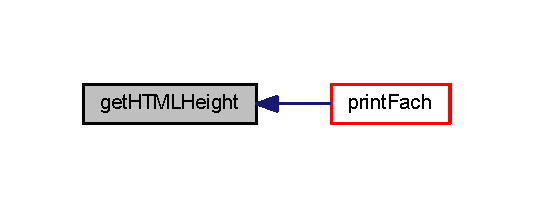
\includegraphics[width=256pt]{classoverview_p_d_f_af41675b946292789cecd9416ca809bcc_icgraph}
\end{center}
\end{figure}


\hypertarget{classoverview_p_d_f_aedc9466cae51e07e57ba865a69c92efc}{\index{overview\+P\+D\+F@{overview\+P\+D\+F}!get\+Next\+Index@{get\+Next\+Index}}
\index{get\+Next\+Index@{get\+Next\+Index}!overview\+P\+D\+F@{overview\+P\+D\+F}}
\paragraph[{get\+Next\+Index}]{\setlength{\rightskip}{0pt plus 5cm}get\+Next\+Index (
\begin{DoxyParamCaption}
\item[{}]{\$i\+Level}
\end{DoxyParamCaption}
)\hspace{0.3cm}{\ttfamily [private]}}}\label{classoverview_p_d_f_aedc9466cae51e07e57ba865a69c92efc}


Gets index of the desired level. 

This utility method manages the \hyperlink{classoverview_p_d_f_a7d055132da646af2b192923c6a864e97}{\$a\+Indices} array and determines what heading index comes next in the given {\ttfamily \$i\+Level} (e.\+g. 1, 2, 3 etc.).

If some levels have been skipped (e.\+g. the first call to this method is with {\ttfamily \$i\+Level = 3}), it fills up the missing array values with 1.

After it has determined the correct index, it increments the corresponding value in the array by 1.


\begin{DoxyParams}[1]{Parameters}
integer & {\em \$i\+Level} & Level for which the index is wanted \\
\hline
\end{DoxyParams}
\begin{DoxyReturn}{Returns}
The next index on the given level. One single integer (i.\+e. not \char`\"{}1.\+1.\+2\char`\"{})
\end{DoxyReturn}
\begin{DoxyAuthor}{Author}
Jakob Strasser -\/ \href{mailto:jakob.strasser@telenet.be}{\tt jakob.\+strasser@telenet.\+be}
\end{DoxyAuthor}
\begin{DoxySince}{Since}
Commit \href{http://github.com/TheJake123/DrupalModul/commit/b9342d941b3f93e212f3f6af0823a07524dd5954}{\tt b9342d9} on 2014-\/06-\/30 
\end{DoxySince}


Definition at line 113 of file pdf\+\_\+creator.\+inc.\+php.



Referenced by print\+Heading().



Here is the caller graph for this function\+:
\nopagebreak
\begin{figure}[H]
\begin{center}
\leavevmode
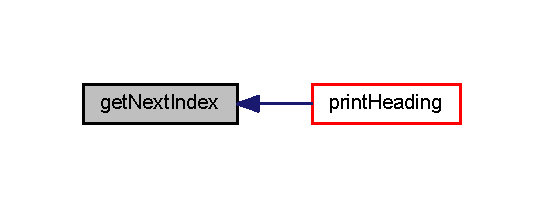
\includegraphics[width=261pt]{classoverview_p_d_f_aedc9466cae51e07e57ba865a69c92efc_icgraph}
\end{center}
\end{figure}


\hypertarget{classoverview_p_d_f_adca20f06977ea2b3b8737b1d465a1606}{\index{overview\+P\+D\+F@{overview\+P\+D\+F}!get\+Total\+Y@{get\+Total\+Y}}
\index{get\+Total\+Y@{get\+Total\+Y}!overview\+P\+D\+F@{overview\+P\+D\+F}}
\paragraph[{get\+Total\+Y}]{\setlength{\rightskip}{0pt plus 5cm}get\+Total\+Y (
\begin{DoxyParamCaption}
{}
\end{DoxyParamCaption}
)\hspace{0.3cm}{\ttfamily [private]}}}\label{classoverview_p_d_f_adca20f06977ea2b3b8737b1d465a1606}


Gets the full y-\/position in the document. 

This utility method determines the current y position in relation to the beginning of the document, not just the current page (like T\+C\+P\+D\+F\+::\+Get\+Y()), excluding top and bottom margins.

This method is needed to compare positions in the document across pages.

\begin{DoxyReturn}{Returns}
Full y-\/position in the entire document (not just on this page), excluding margins
\end{DoxyReturn}
\begin{DoxyAuthor}{Author}
Jakob Strasser -\/ \href{mailto:jakob.strasser@telenet.be}{\tt jakob.\+strasser@telenet.\+be} 
\end{DoxyAuthor}
\begin{DoxySince}{Since}
Commit \href{http://github.com/TheJake123/DrupalModul/commit/b9342d941b3f93e212f3f6af0823a07524dd5954}{\tt b9342d9} on 2014-\/06-\/30
\end{DoxySince}
\begin{DoxySeeAlso}{See also}
\hyperlink{classoverview_p_d_f_af41675b946292789cecd9416ca809bcc}{get\+H\+T\+M\+L\+Height()} 

T\+C\+P\+D\+F\+::\+Get\+Y() 
\end{DoxySeeAlso}


Definition at line 168 of file pdf\+\_\+creator.\+inc.\+php.

\hypertarget{classoverview_p_d_f_a10c644f1f84ae1b261a8b198a66b5cb1}{\index{overview\+P\+D\+F@{overview\+P\+D\+F}!get\+Unique\+Filename@{get\+Unique\+Filename}}
\index{get\+Unique\+Filename@{get\+Unique\+Filename}!overview\+P\+D\+F@{overview\+P\+D\+F}}
\paragraph[{get\+Unique\+Filename}]{\setlength{\rightskip}{0pt plus 5cm}get\+Unique\+Filename (
\begin{DoxyParamCaption}
\item[{}]{\$s\+Curr\+Type, }
\item[{}]{\$s\+Curr\+Version}
\end{DoxyParamCaption}
)\hspace{0.3cm}{\ttfamily [private]}}}\label{classoverview_p_d_f_a10c644f1f84ae1b261a8b198a66b5cb1}


Creates a unique filename. 

Determines if a file with the standard filename as defined in the module settings already exists. If one exists, it appends a number and increases it until the name is not already taken.

Also, it creates the directory into which the document should be saved according to the module settings (if it does not already exist).


\begin{DoxyParams}[1]{Parameters}
string & {\em \$s\+Curr\+Type} & The type of the curriculum (Bachelorstudium, Masterstudium) \\
\hline
string & {\em \$s\+Curr\+Version} & The version of the curriculum (e.\+g. 2013\+W) \\
\hline
\end{DoxyParams}
\begin{DoxyReturn}{Returns}
The unique filename
\end{DoxyReturn}
\begin{DoxyAuthor}{Author}
Jakob Strasser -\/ \href{mailto:jakob.strasser@telenet.be}{\tt jakob.\+strasser@telenet.\+be} 
\end{DoxyAuthor}
\begin{DoxySince}{Since}
Commit \href{http://github.com/TheJake123/DrupalModul/commit/e8704fdc454e3db61b5be799b2d4928b7bfb6686}{\tt e8704fd} on 2014-\/06-\/30
\end{DoxySince}
\begin{DoxySeeAlso}{See also}
\hyperlink{group___stukowin___module_ga55d453d5b6f8ae4e643308d8814e67a5}{stukowin\+\_\+admin()} 
\end{DoxySeeAlso}


Definition at line 291 of file pdf\+\_\+creator.\+inc.\+php.



References convert\+String\+To\+Valid\+Filename().



Here is the call graph for this function\+:
\nopagebreak
\begin{figure}[H]
\begin{center}
\leavevmode
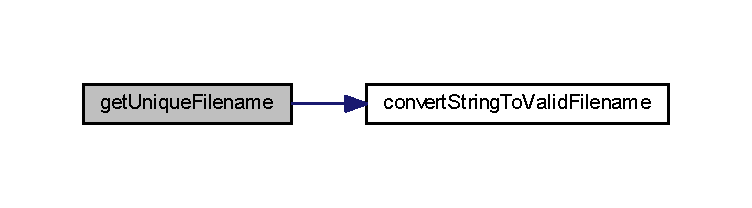
\includegraphics[width=350pt]{classoverview_p_d_f_a10c644f1f84ae1b261a8b198a66b5cb1_cgraph}
\end{center}
\end{figure}


\hypertarget{classoverview_p_d_f_a1871e6880b3bb67d0a49cdcab4cd680d}{\index{overview\+P\+D\+F@{overview\+P\+D\+F}!print\+Curriculum@{print\+Curriculum}}
\index{print\+Curriculum@{print\+Curriculum}!overview\+P\+D\+F@{overview\+P\+D\+F}}
\paragraph[{print\+Curriculum}]{\setlength{\rightskip}{0pt plus 5cm}print\+Curriculum (
\begin{DoxyParamCaption}
\item[{}]{\$o\+Curriculum}
\end{DoxyParamCaption}
)\hspace{0.3cm}{\ttfamily [private]}}}\label{classoverview_p_d_f_a1871e6880b3bb67d0a49cdcab4cd680d}


Prints a curriculum object and all its courses to the P\+D\+F document. 

This method does the following things\+:
\begin{DoxyEnumerate}
\item Print the curriculum name as a heading
\item Create an overview table with all the subjects it contains
\item Print the details of each subject to the document
\end{DoxyEnumerate}


\begin{DoxyParams}[1]{Parameters}
object & {\em \$o\+Curriculum} & The curriculum object to print\\
\hline
\end{DoxyParams}
\begin{DoxyAuthor}{Author}
Jakob Strasser -\/ \href{mailto:jakob.strasser@telenet.be}{\tt jakob.\+strasser@telenet.\+be} 
\end{DoxyAuthor}
\begin{DoxySince}{Since}
Commit \href{http://github.com/TheJake123/DrupalModul/commit/b9342d941b3f93e212f3f6af0823a07524dd5954}{\tt b9342d9} on 2014-\/06-\/30 
\end{DoxySince}


Definition at line 328 of file pdf\+\_\+creator.\+inc.\+php.



References get\+Courses(), print\+Heading(), and print\+Top\+Level().



Referenced by create\+P\+D\+F().



Here is the call graph for this function\+:
\nopagebreak
\begin{figure}[H]
\begin{center}
\leavevmode
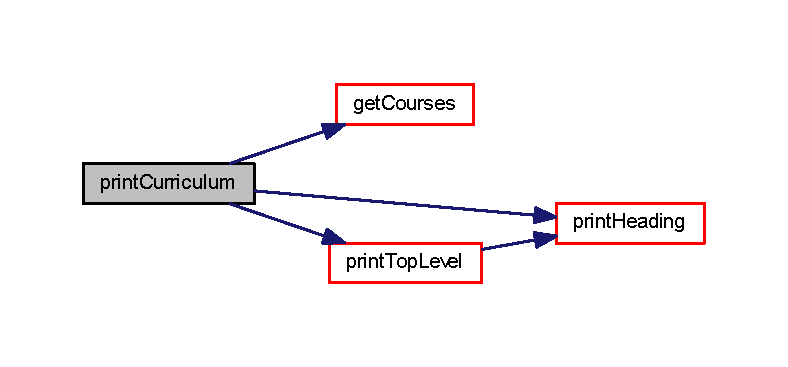
\includegraphics[width=350pt]{classoverview_p_d_f_a1871e6880b3bb67d0a49cdcab4cd680d_cgraph}
\end{center}
\end{figure}




Here is the caller graph for this function\+:
\nopagebreak
\begin{figure}[H]
\begin{center}
\leavevmode
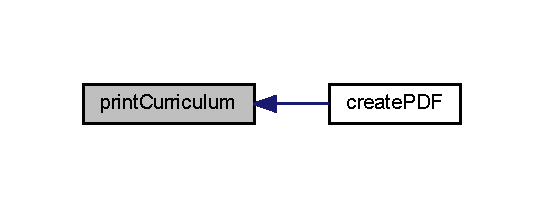
\includegraphics[width=261pt]{classoverview_p_d_f_a1871e6880b3bb67d0a49cdcab4cd680d_icgraph}
\end{center}
\end{figure}


\hypertarget{classoverview_p_d_f_abf0674d88080affc25c472fbd0525896}{\index{overview\+P\+D\+F@{overview\+P\+D\+F}!print\+Fach@{print\+Fach}}
\index{print\+Fach@{print\+Fach}!overview\+P\+D\+F@{overview\+P\+D\+F}}
\paragraph[{print\+Fach}]{\setlength{\rightskip}{0pt plus 5cm}print\+Fach (
\begin{DoxyParamCaption}
\item[{}]{\$o\+Fach}
\end{DoxyParamCaption}
)\hspace{0.3cm}{\ttfamily [private]}}}\label{classoverview_p_d_f_abf0674d88080affc25c472fbd0525896}


Prints a subject to the P\+D\+F document. 

This method prints the subject title and details, an overview of all its subcourses and their details to the document.


\begin{DoxyParams}[1]{Parameters}
object & {\em \$o\+Fach} & The course object to print\\
\hline
\end{DoxyParams}
\begin{DoxyAuthor}{Author}
Jakob Strasser -\/ \href{mailto:jakob.strasser@telenet.be}{\tt jakob.\+strasser@telenet.\+be} 
\end{DoxyAuthor}
\begin{DoxySince}{Since}
Commit \href{http://github.com/TheJake123/DrupalModul/commit/b9342d941b3f93e212f3f6af0823a07524dd5954}{\tt b9342d9} on 2014-\/06-\/30 
\end{DoxySince}


Definition at line 398 of file pdf\+\_\+creator.\+inc.\+php.



References generate\+Table\+Rec\+Helper(), get\+H\+T\+M\+L\+Height(), print\+Heading(), and print\+Ziele\+Inhalte().



Referenced by print\+Top\+Level().



Here is the call graph for this function\+:
\nopagebreak
\begin{figure}[H]
\begin{center}
\leavevmode
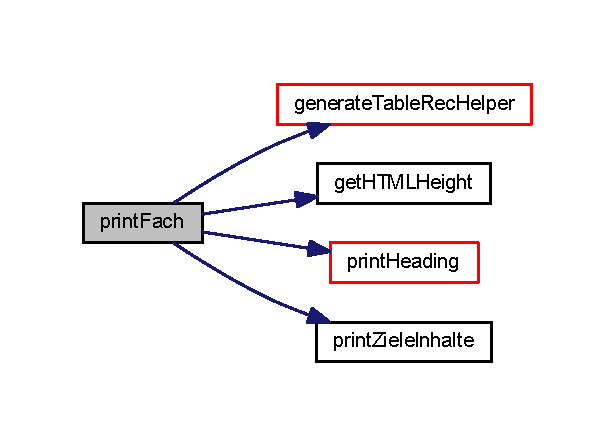
\includegraphics[width=295pt]{classoverview_p_d_f_abf0674d88080affc25c472fbd0525896_cgraph}
\end{center}
\end{figure}




Here is the caller graph for this function\+:
\nopagebreak
\begin{figure}[H]
\begin{center}
\leavevmode
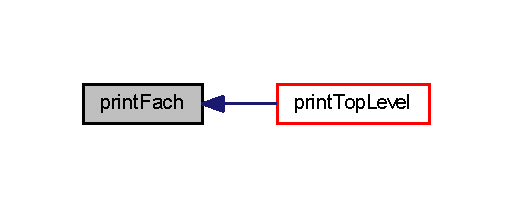
\includegraphics[width=246pt]{classoverview_p_d_f_abf0674d88080affc25c472fbd0525896_icgraph}
\end{center}
\end{figure}


\hypertarget{classoverview_p_d_f_ad6b57d30526fb658521faddce7595dc4}{\index{overview\+P\+D\+F@{overview\+P\+D\+F}!print\+Heading@{print\+Heading}}
\index{print\+Heading@{print\+Heading}!overview\+P\+D\+F@{overview\+P\+D\+F}}
\paragraph[{print\+Heading}]{\setlength{\rightskip}{0pt plus 5cm}print\+Heading (
\begin{DoxyParamCaption}
\item[{}]{\$s\+Text, }
\item[{}]{\$i\+Level, }
\item[{}]{\$b\+Show\+Index = {\ttfamily true}, }
\item[{}]{\$s\+Align = {\ttfamily 'L'}, }
\item[{}]{\$b\+Add\+Bookmark = {\ttfamily true}}
\end{DoxyParamCaption}
)\hspace{0.3cm}{\ttfamily [private]}}}\label{classoverview_p_d_f_ad6b57d30526fb658521faddce7595dc4}


Prints a heading to the P\+D\+F document. 

This method manages headings in the document. It automatically indexes the headings using \hyperlink{classoverview_p_d_f_aedc9466cae51e07e57ba865a69c92efc}{get\+Next\+Index()} and optionally adds a bookmark for it.


\begin{DoxyParams}[1]{Parameters}
string & {\em \$s\+Text} & The heading text \\
\hline
int & {\em \$i\+Level} & The level at which the heading should be created and the bookmark set \\
\hline
boolean & {\em \$b\+Show\+Index} & {\ttfamily true} if the index should be shown in the heading \\
\hline
string & {\em \$s\+Align} & Alignment of the heading. For allowed values see T\+C\+P\+D\+F\+::\+Multi\+Cell() \\
\hline
boolean & {\em \$b\+Add\+Bookmark} & {\ttfamily true} if heading should be shown on the index page and bookmarked\\
\hline
\end{DoxyParams}
\begin{DoxyAuthor}{Author}
Jakob Strasser -\/ \href{mailto:jakob.strasser@telenet.be}{\tt jakob.\+strasser@telenet.\+be} 
\end{DoxyAuthor}
\begin{DoxySince}{Since}
Commit \href{http://github.com/TheJake123/DrupalModul/commit/b9342d941b3f93e212f3f6af0823a07524dd5954}{\tt b9342d9} on 2014-\/06-\/30
\end{DoxySince}
\begin{DoxySeeAlso}{See also}
\hyperlink{classoverview_p_d_f_acf4bdf38a6e11c036b076a16c3516f75}{create\+T\+O\+C\+Page()} 

\hyperlink{classoverview_p_d_f_aedc9466cae51e07e57ba865a69c92efc}{get\+Next\+Index()} 
\end{DoxySeeAlso}


Definition at line 587 of file pdf\+\_\+creator.\+inc.\+php.



References get\+Next\+Index().



Referenced by print\+Curriculum(), print\+Fach(), and print\+Top\+Level().



Here is the call graph for this function\+:
\nopagebreak
\begin{figure}[H]
\begin{center}
\leavevmode
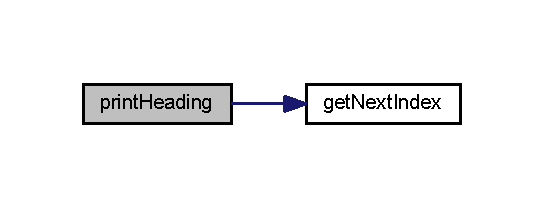
\includegraphics[width=261pt]{classoverview_p_d_f_ad6b57d30526fb658521faddce7595dc4_cgraph}
\end{center}
\end{figure}




Here is the caller graph for this function\+:
\nopagebreak
\begin{figure}[H]
\begin{center}
\leavevmode
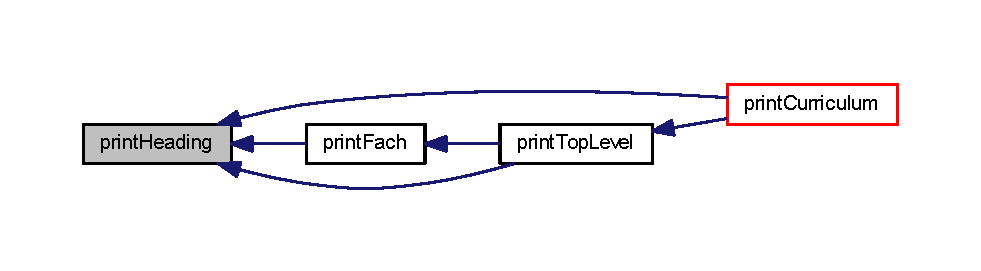
\includegraphics[width=350pt]{classoverview_p_d_f_ad6b57d30526fb658521faddce7595dc4_icgraph}
\end{center}
\end{figure}


\hypertarget{classoverview_p_d_f_a23c7451efb8c436590fbad032bc6788b}{\index{overview\+P\+D\+F@{overview\+P\+D\+F}!print\+Top\+Level@{print\+Top\+Level}}
\index{print\+Top\+Level@{print\+Top\+Level}!overview\+P\+D\+F@{overview\+P\+D\+F}}
\paragraph[{print\+Top\+Level}]{\setlength{\rightskip}{0pt plus 5cm}print\+Top\+Level (
\begin{DoxyParamCaption}
\item[{}]{\$o\+Top\+Level}
\end{DoxyParamCaption}
)\hspace{0.3cm}{\ttfamily [private]}}}\label{classoverview_p_d_f_a23c7451efb8c436590fbad032bc6788b}


Decides whether to print a structural element or a subject. 

This is a dispatcher method that checks if an object is a structural element (1. Semester, 2. Semester etc.) or a course. If calls \hyperlink{classoverview_p_d_f_ad6b57d30526fb658521faddce7595dc4}{print\+Heading()} if it is a structural element and then \hyperlink{classoverview_p_d_f_abf0674d88080affc25c472fbd0525896}{print\+Fach()} for all its children or just \hyperlink{classoverview_p_d_f_abf0674d88080affc25c472fbd0525896}{print\+Fach()} if it is a course object.


\begin{DoxyParams}[1]{Parameters}
object & {\em \$o\+Top\+Level} & The object to check\\
\hline
\end{DoxyParams}
\begin{DoxyAuthor}{Author}
Jakob Strasser -\/ \href{mailto:jakob.strasser@telenet.be}{\tt jakob.\+strasser@telenet.\+be} 
\end{DoxyAuthor}
\begin{DoxySince}{Since}
Commit \href{http://github.com/TheJake123/DrupalModul/commit/a311596e0d6f1d08314cfcbc9f4f878a131a3f61}{\tt a311596} on 2014-\/07-\/02 
\end{DoxySince}


Definition at line 376 of file pdf\+\_\+creator.\+inc.\+php.



References print\+Fach(), and print\+Heading().



Referenced by print\+Curriculum().



Here is the call graph for this function\+:
\nopagebreak
\begin{figure}[H]
\begin{center}
\leavevmode
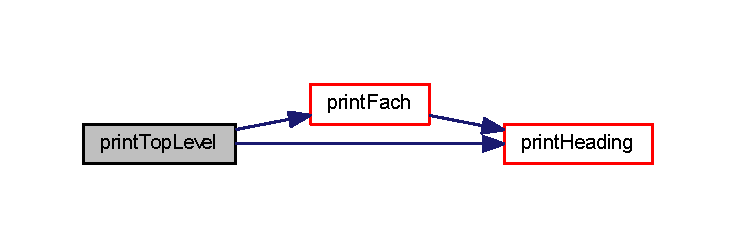
\includegraphics[width=350pt]{classoverview_p_d_f_a23c7451efb8c436590fbad032bc6788b_cgraph}
\end{center}
\end{figure}




Here is the caller graph for this function\+:
\nopagebreak
\begin{figure}[H]
\begin{center}
\leavevmode
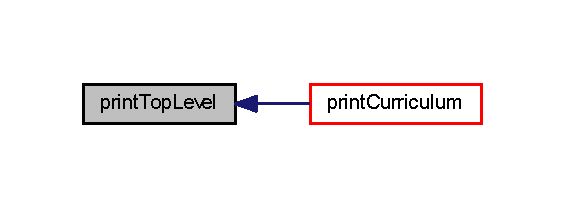
\includegraphics[width=271pt]{classoverview_p_d_f_a23c7451efb8c436590fbad032bc6788b_icgraph}
\end{center}
\end{figure}


\hypertarget{classoverview_p_d_f_af0b14d64b47fe81df7965b8259ccb762}{\index{overview\+P\+D\+F@{overview\+P\+D\+F}!print\+Ziele\+Inhalte@{print\+Ziele\+Inhalte}}
\index{print\+Ziele\+Inhalte@{print\+Ziele\+Inhalte}!overview\+P\+D\+F@{overview\+P\+D\+F}}
\paragraph[{print\+Ziele\+Inhalte}]{\setlength{\rightskip}{0pt plus 5cm}print\+Ziele\+Inhalte (
\begin{DoxyParamCaption}
\item[{}]{\$o\+Course}
\end{DoxyParamCaption}
)\hspace{0.3cm}{\ttfamily [private]}}}\label{classoverview_p_d_f_af0b14d64b47fe81df7965b8259ccb762}


Prints the course goals and content of teaching and their respecitve headings to the document. 

If one of them is not set or empty, their heading is not printed either.


\begin{DoxyParams}[1]{Parameters}
object & {\em \$o\+Course} & The course to print the goals and contents for\\
\hline
\end{DoxyParams}
\begin{DoxyAuthor}{Author}
Jakob Strasser -\/ \href{mailto:jakob.strasser@telenet.be}{\tt jakob.\+strasser@telenet.\+be} 
\end{DoxyAuthor}
\begin{DoxySince}{Since}
Commit \href{http://github.com/TheJake123/DrupalModul/commit/b9342d941b3f93e212f3f6af0823a07524dd5954}{\tt b9342d9} on 2014-\/06-\/30
\end{DoxySince}
\begin{DoxySeeAlso}{See also}
\hyperlink{classoverview_p_d_f_abf0674d88080affc25c472fbd0525896}{print\+Fach()} 
\end{DoxySeeAlso}


Definition at line 546 of file pdf\+\_\+creator.\+inc.\+php.



Referenced by print\+Fach().



Here is the caller graph for this function\+:
\nopagebreak
\begin{figure}[H]
\begin{center}
\leavevmode
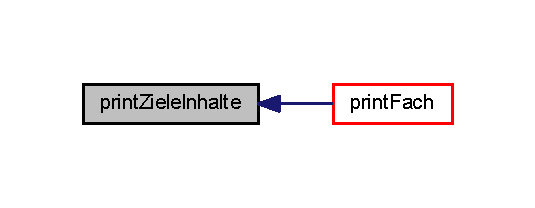
\includegraphics[width=257pt]{classoverview_p_d_f_af0b14d64b47fe81df7965b8259ccb762_icgraph}
\end{center}
\end{figure}


\hypertarget{classoverview_p_d_f_aa12feabadc0d4aa85bb4da7454f8245d}{\index{overview\+P\+D\+F@{overview\+P\+D\+F}!split\+Bold\+Text\+Into\+Lines@{split\+Bold\+Text\+Into\+Lines}}
\index{split\+Bold\+Text\+Into\+Lines@{split\+Bold\+Text\+Into\+Lines}!overview\+P\+D\+F@{overview\+P\+D\+F}}
\paragraph[{split\+Bold\+Text\+Into\+Lines}]{\setlength{\rightskip}{0pt plus 5cm}split\+Bold\+Text\+Into\+Lines (
\begin{DoxyParamCaption}
\item[{}]{\$s\+Text, }
\item[{}]{\$i\+Max\+Width}
\end{DoxyParamCaption}
)\hspace{0.3cm}{\ttfamily [private]}}}\label{classoverview_p_d_f_aa12feabadc0d4aa85bb4da7454f8245d}


Inserts line breaks into bold text. 

This method breaks the {\itshape \$s\+Text} into separate lines which are shorter than {\itshape \$i\+Max\+Width} if printed as bold text. If one word alone is too long or the entire string is shorter than {\itshape \$i\+Max\+Width}, it is not splitted.

This method is needed in \hyperlink{classoverview_p_d_f_ad0ea6c6476d690b08161300e40926dc6}{generate\+Table\+Rec\+Helper()} because \hyperlink{class_t_c_p_d_f}{T\+C\+P\+D\+F} does not break the words correctly in a table if the text is written in a $<$B$>$ tag. This caused issues where text would overflow its table cell to the right by a few cm.


\begin{DoxyParams}[1]{Parameters}
string & {\em \$s\+Text} & The text to split \\
\hline
 & {\em \$i\+Max\+Width} & The The maximum width a line is allowed to have \\
\hline
\end{DoxyParams}
\begin{DoxyReturn}{Returns}
The {\itshape \$s\+Text} with $<$br$>$ tags inserted whenever necessary
\end{DoxyReturn}
\begin{DoxyAuthor}{Author}
Jakob Strasser -\/ \href{mailto:jakob.strasser@telenet.be}{\tt jakob.\+strasser@telenet.\+be} 
\end{DoxyAuthor}
\begin{DoxySince}{Since}
Commit \href{http://github.com/TheJake123/DrupalModul/commit/7e5b545971fbee0bb6140cf3fef51185bf86c94e}{\tt 7e5b545} on 2014-\/07-\/06 
\end{DoxySince}


Definition at line 498 of file pdf\+\_\+creator.\+inc.\+php.



References split\+Rec\+Helper().



Referenced by generate\+Table\+Rec\+Helper().



Here is the call graph for this function\+:
\nopagebreak
\begin{figure}[H]
\begin{center}
\leavevmode
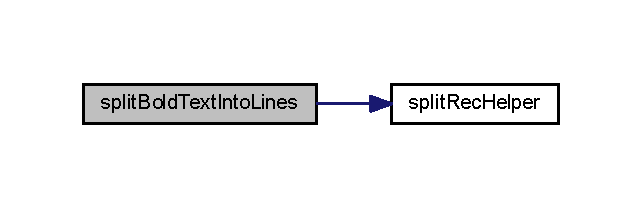
\includegraphics[width=308pt]{classoverview_p_d_f_aa12feabadc0d4aa85bb4da7454f8245d_cgraph}
\end{center}
\end{figure}




Here is the caller graph for this function\+:
\nopagebreak
\begin{figure}[H]
\begin{center}
\leavevmode
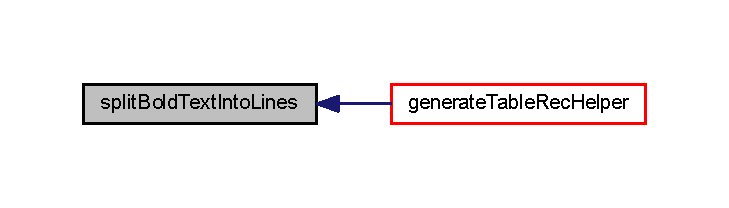
\includegraphics[width=350pt]{classoverview_p_d_f_aa12feabadc0d4aa85bb4da7454f8245d_icgraph}
\end{center}
\end{figure}


\hypertarget{classoverview_p_d_f_af3f9a49de14251ba45bd046879f27aa2}{\index{overview\+P\+D\+F@{overview\+P\+D\+F}!split\+Rec\+Helper@{split\+Rec\+Helper}}
\index{split\+Rec\+Helper@{split\+Rec\+Helper}!overview\+P\+D\+F@{overview\+P\+D\+F}}
\paragraph[{split\+Rec\+Helper}]{\setlength{\rightskip}{0pt plus 5cm}split\+Rec\+Helper (
\begin{DoxyParamCaption}
\item[{}]{\$a\+Words, }
\item[{}]{\$i\+Curr\+Index, }
\item[{}]{\$i\+Max\+Width}
\end{DoxyParamCaption}
)\hspace{0.3cm}{\ttfamily [private]}}}\label{classoverview_p_d_f_af3f9a49de14251ba45bd046879f27aa2}


Recursive helper function for \hyperlink{classoverview_p_d_f_aa12feabadc0d4aa85bb4da7454f8245d}{split\+Bold\+Text\+Into\+Lines()} 


\begin{DoxyParams}[1]{Parameters}
array & {\em \$a\+Words} & The array of words as split in \hyperlink{classoverview_p_d_f_aa12feabadc0d4aa85bb4da7454f8245d}{split\+Bold\+Text\+Into\+Lines()} \\
\hline
integer & {\em \$i\+Curr\+Index} & The current index in the array \\
\hline
integer & {\em \$i\+Max\+Width} & The maximum width a line is allowed to have\\
\hline
\end{DoxyParams}
\begin{DoxyAuthor}{Author}
Jakob Strasser -\/ \href{mailto:jakob.strasser@telenet.be}{\tt jakob.\+strasser@telenet.\+be} 
\end{DoxyAuthor}
\begin{DoxySince}{Since}
Commit \href{http://github.com/TheJake123/DrupalModul/commit/7e5b545971fbee0bb6140cf3fef51185bf86c94e}{\tt 7e5b545} on 2014-\/07-\/06
\end{DoxySince}
\begin{DoxySeeAlso}{See also}
\hyperlink{classoverview_p_d_f_aa12feabadc0d4aa85bb4da7454f8245d}{split\+Bold\+Text\+Into\+Lines()} 
\end{DoxySeeAlso}


Definition at line 520 of file pdf\+\_\+creator.\+inc.\+php.



Referenced by split\+Bold\+Text\+Into\+Lines().



Here is the caller graph for this function\+:
\nopagebreak
\begin{figure}[H]
\begin{center}
\leavevmode
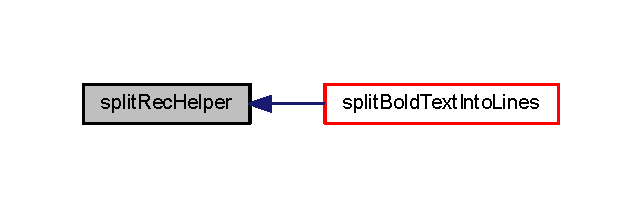
\includegraphics[width=308pt]{classoverview_p_d_f_af3f9a49de14251ba45bd046879f27aa2_icgraph}
\end{center}
\end{figure}




\subsubsection{Field Documentation}
\hypertarget{classoverview_p_d_f_a7d055132da646af2b192923c6a864e97}{\index{overview\+P\+D\+F@{overview\+P\+D\+F}!\$a\+Indices@{\$a\+Indices}}
\index{\$a\+Indices@{\$a\+Indices}!overview\+P\+D\+F@{overview\+P\+D\+F}}
\paragraph[{\$a\+Indices}]{\setlength{\rightskip}{0pt plus 5cm}\$a\+Indices = array ()\hspace{0.3cm}{\ttfamily [private]}}}\label{classoverview_p_d_f_a7d055132da646af2b192923c6a864e97}


Array of indices for continuous indexation of headings. 

Every key in this array represents an indexation level (e.\+g. level 2 for 1.\+1, level 3 for 1.\+1.\+1) and every value in the array the current index for that level.

\begin{DoxySince}{Since}
Commit \href{http://github.com/TheJake123/DrupalModul/commit/b9342d941b3f93e212f3f6af0823a07524dd5954}{\tt b9342d9} on 2014-\/06-\/30 
\end{DoxySince}
\begin{DoxySeeAlso}{See also}
\hyperlink{classoverview_p_d_f_aedc9466cae51e07e57ba865a69c92efc}{get\+Next\+Index()} 
\end{DoxySeeAlso}


Definition at line 73 of file pdf\+\_\+creator.\+inc.\+php.



The documentation for this class was generated from the following file\+:\begin{DoxyCompactItemize}
\item 
\hyperlink{pdf__creator_8inc_8php}{pdf\+\_\+creator.\+inc.\+php}\end{DoxyCompactItemize}

\hypertarget{class_t_c_p_d_f}{\subsection{T\+C\+P\+D\+F Class Reference}
\label{class_t_c_p_d_f}\index{T\+C\+P\+D\+F@{T\+C\+P\+D\+F}}
}


Inheritance diagram for T\+C\+P\+D\+F\+:
\nopagebreak
\begin{figure}[H]
\begin{center}
\leavevmode
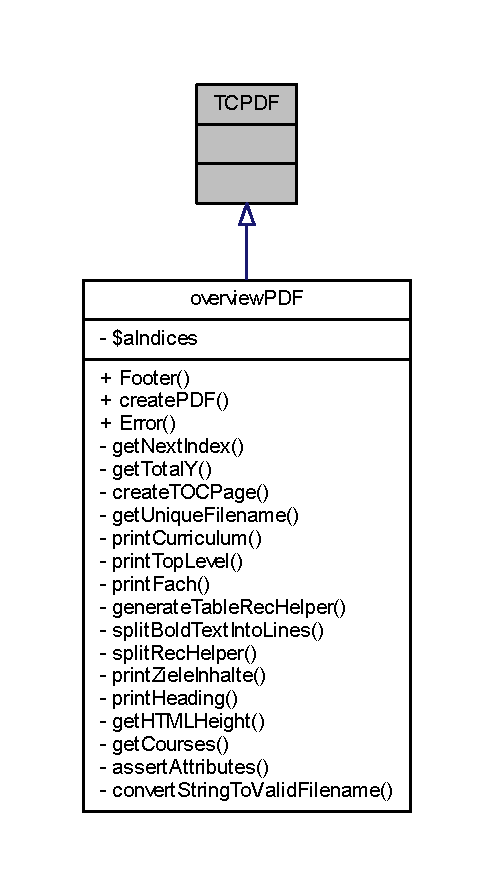
\includegraphics[width=237pt]{class_t_c_p_d_f__inherit__graph}
\end{center}
\end{figure}


The documentation for this class was generated from the following file\+:\begin{DoxyCompactItemize}
\item 
\hyperlink{pdf__creator_8inc_8php}{pdf\+\_\+creator.\+inc.\+php}\end{DoxyCompactItemize}

\section{File Documentation}
\hypertarget{ceus__importer_8inc_8php}{\subsection{ceus\+\_\+importer.\+inc.\+php File Reference}
\label{ceus__importer_8inc_8php}\index{ceus\+\_\+importer.\+inc.\+php@{ceus\+\_\+importer.\+inc.\+php}}
}


Imports data from C\+E\+U\+S.  


\subsubsection*{Data Structures}
\begin{DoxyCompactItemize}
\item 
class \hyperlink{classceus__importer}{ceus\+\_\+importer}
\begin{DoxyCompactList}\small\item\em Imports data from C\+E\+U\+S and stores it in the Drupal database. \end{DoxyCompactList}\end{DoxyCompactItemize}


\subsubsection{Detailed Description}
Imports data from C\+E\+U\+S. 

This file manages the import of curricula data from C\+E\+U\+S.

\begin{DoxyAuthor}{Author}
Konstantinos Dafalias -\/ \href{mailto:kdafalias@gmail.com}{\tt kdafalias@gmail.\+com} 
\end{DoxyAuthor}
\begin{DoxyAuthor}{Authors}
Jakob Strasser -\/ \href{mailto:jakob.strasser@telenet.be}{\tt jakob.\+strasser@telenet.\+be} 

Markus Gutmayer -\/ \href{mailto:m.gutmayer@gmail.com}{\tt m.\+gutmayer@gmail.\+com} 

Werner Breuer -\/ \href{mailto:bluescreenwerner@gmail.com}{\tt bluescreenwerner@gmail.\+com} 
\end{DoxyAuthor}
\begin{DoxyVersion}{Version}
1.\+0.\+0 2014-\/07-\/16 
\end{DoxyVersion}
\begin{DoxySince}{Since}
Commit \href{http://github.com/TheJake123/DrupalModul/commit/d179abcc5e05743086cd67cf1ce30b08923a7183}{\tt d179abc} on 2014-\/06-\/28 
\end{DoxySince}


Definition in file \hyperlink{ceus__importer_8inc_8php_source}{ceus\+\_\+importer.\+inc.\+php}.


\hypertarget{content__manager_8inc_8php}{\subsection{content\+\_\+manager.\+inc.\+php File Reference}
\label{content__manager_8inc_8php}\index{content\+\_\+manager.\+inc.\+php@{content\+\_\+manager.\+inc.\+php}}
}


Access to curricula data.  


\subsubsection*{Data Structures}
\begin{DoxyCompactItemize}
\item 
class \hyperlink{classcontent__manager}{content\+\_\+manager}
\begin{DoxyCompactList}\small\item\em Access to drupal vocabularies and content nodes. \end{DoxyCompactList}\end{DoxyCompactItemize}


\subsubsection{Detailed Description}
Access to curricula data. 

This file contains all necessary functionality for accessing the curricula data stored in drupal

\begin{DoxyAuthor}{Authors}
Werner Breuer -\/ \href{mailto:bluescreenwerner@gmail.com}{\tt bluescreenwerner@gmail.\+com} 

Konstantinos Dafalias -\/ \href{mailto:kdafalias@gmail.com}{\tt kdafalias@gmail.\+com} 

Jakob Strasser -\/ \href{mailto:jakob.strasser@telenet.be}{\tt jakob.\+strasser@telenet.\+be} 
\end{DoxyAuthor}
\begin{DoxyVersion}{Version}
1.\+0.\+0 2014-\/07-\/07 
\end{DoxyVersion}
\begin{DoxySince}{Since}
Commit \href{http://github.com/TheJake123/DrupalModul/commit/f90560aa796b39853beb42a521d6d94c86051c46}{\tt f90560a} on 2014-\/06-\/28
\end{DoxySince}
\begin{DoxySeeAlso}{See also}
\hyperlink{classcontent__manager}{content\+\_\+manager} 
\end{DoxySeeAlso}


Definition in file \hyperlink{content__manager_8inc_8php_source}{content\+\_\+manager.\+inc.\+php}.


\hypertarget{exparse_8h}{\subsection{exparse.\+h File Reference}
\label{exparse_8h}\index{exparse.\+h@{exparse.\+h}}
}
\subsubsection*{Data Structures}
\begin{DoxyCompactItemize}
\item 
union \hyperlink{union_e_x_s_t_y_p_e}{E\+X\+S\+T\+Y\+P\+E}
\end{DoxyCompactItemize}
\subsubsection*{Macros}
\begin{DoxyCompactItemize}
\item 
\#define \hyperlink{exparse_8h_acd0c2c3f440bd9f1ffc39e6e0a3b1ecd}{E\+X\+T\+O\+K\+E\+N\+T\+Y\+P\+E}
\item 
\#define \hyperlink{exparse_8h_a3d7aad03a0b987d400ede576235dedd1}{M\+I\+N\+T\+O\+K\+E\+N}~258
\item 
\#define \hyperlink{exparse_8h_a91d43eadec33c80149f92e5abf5df58c}{I\+N\+T\+E\+G\+E\+R}~259
\item 
\#define \hyperlink{exparse_8h_a08cbc66092284f7da94279f986a0aae9}{U\+N\+S\+I\+G\+N\+E\+D}~260
\item 
\#define \hyperlink{exparse_8h_a1318901e3fc847acae31155c47e28630}{C\+H\+A\+R\+A\+C\+T\+E\+R}~261
\item 
\#define \hyperlink{exparse_8h_a651fd7cc9bac84def593adaf5d2ae84d}{F\+L\+O\+A\+T\+I\+N\+G}~262
\item 
\#define \hyperlink{exparse_8h_a0f4d394a3ab4e09bff60f714c66dc5ee}{S\+T\+R\+I\+N\+G}~263
\item 
\#define \hyperlink{exparse_8h_a75bfd14b4b0ebac12ba08b9b36229225}{V\+O\+I\+D\+T\+Y\+P\+E}~264
\item 
\#define \hyperlink{exparse_8h_a280feb883e9d4a7edcc69c8bcb9f38f2}{A\+D\+D\+R\+E\+S\+S}~265
\item 
\#define \hyperlink{exparse_8h_af579248b8d4c16c0aeba3dff9ee8b10a}{A\+R\+R\+A\+Y}~266
\item 
\#define \hyperlink{exparse_8h_abe022c8f09db1f0680a92293523f25dd}{B\+R\+E\+A\+K}~267
\item 
\#define \hyperlink{exparse_8h_aa980b5e5e502cf62bdca6c0452b97516}{C\+A\+L\+L}~268
\item 
\#define \hyperlink{exparse_8h_af2b30344be261ffe1c5aad12ab1f6f07}{C\+A\+S\+E}~269
\item 
\#define \hyperlink{exparse_8h_aa07f83a2de5a158b8643cdc36541b711}{C\+O\+N\+S\+T\+A\+N\+T}~270
\item 
\#define \hyperlink{exparse_8h_ab711666ad09d7f6c0b91576525ea158e}{C\+O\+N\+T\+I\+N\+U\+E}~271
\item 
\#define \hyperlink{exparse_8h_ad06c120bb4a679d1c90ce7313f40e3ac}{D\+E\+C\+L\+A\+R\+E}~272
\item 
\#define \hyperlink{exparse_8h_a3da44afeba217135a680a7477b5e3ce3}{D\+E\+F\+A\+U\+L\+T}~273
\item 
\#define \hyperlink{exparse_8h_a135001d5360c2c2472130ada2d26c65e}{D\+Y\+N\+A\+M\+I\+C}~274
\item 
\#define \hyperlink{exparse_8h_a0a70ee0cbf5b1738be4c9463c529ce72}{E\+L\+S\+E}~275
\item 
\#define \hyperlink{exparse_8h_ad111e603bbebe5d87f6bc39264ce4733}{E\+X\+I\+T}~276
\item 
\#define \hyperlink{exparse_8h_a6634515171060cf2f7afd70a96cb9bde}{F\+O\+R}~277
\item 
\#define \hyperlink{exparse_8h_aee0cf83ee6d754df700e396da8987f1f}{F\+U\+N\+C\+T\+I\+O\+N}~278
\item 
\#define \hyperlink{exparse_8h_aa9e6883d671f2458cec1698d98a348bd}{G\+S\+U\+B}~279
\item 
\#define \hyperlink{exparse_8h_a565fde10770e8a57ef907f3f4f991ea2}{I\+T\+E\+R\+A\+T\+E}~280
\item 
\#define \hyperlink{exparse_8h_a45f3a5655265d311729c47181f2094cd}{I\+T\+E\+R\+A\+T\+E\+R}~281
\item 
\#define \hyperlink{exparse_8h_a77ceac8d6af195fe72f95f6afd87c45e}{I\+D}~282
\item 
\#define \hyperlink{exparse_8h_ac138c68a0709c57bc5f7567abc1558eb}{I\+F}~283
\item 
\#define \hyperlink{exparse_8h_a0b7df70d4a086a227bc482b07e2bbbca}{L\+A\+B\+E\+L}~284
\item 
\#define \hyperlink{exparse_8h_aa52ae0448e8215abe6a23dbf094ade02}{M\+E\+M\+B\+E\+R}~285
\item 
\#define \hyperlink{exparse_8h_a47f2e62c0dbebc787052c165afcada0e}{N\+A\+M\+E}~286
\item 
\#define \hyperlink{exparse_8h_a63cb3834e6075ddad87f8ce324e53988}{P\+O\+S}~287
\item 
\#define \hyperlink{exparse_8h_aac0ed3e151f909c1b30db30b14cd0551}{P\+R\+A\+G\+M\+A}~288
\item 
\#define \hyperlink{exparse_8h_a349316092037fdd0773335fab4e15ee8}{P\+R\+E}~289
\item 
\#define \hyperlink{exparse_8h_a8b43bafee90b30676faae508c21cb8d7}{P\+R\+I\+N\+T}~290
\item 
\#define \hyperlink{exparse_8h_ae1649fc947ca37a86917a08354f48d1a}{P\+R\+I\+N\+T\+F}~291
\item 
\#define \hyperlink{exparse_8h_ac144bb8db6432fb2773aeb05ae17829a}{P\+R\+O\+C\+E\+D\+U\+R\+E}~292
\item 
\#define \hyperlink{exparse_8h_ae5ff1f63e632fba61c45cfb0a2b19066}{Q\+U\+E\+R\+Y}~293
\item 
\#define \hyperlink{exparse_8h_a839a9222721835f53c5b248241f535f4}{R\+A\+N\+D}~294
\item 
\#define \hyperlink{exparse_8h_a6a0e6b80dd3d5ca395cf58151749f5e2}{R\+E\+T\+U\+R\+N}~295
\item 
\#define \hyperlink{exparse_8h_a1799711cd7a7b727846cfe2068f67c66}{S\+C\+A\+N\+F}~296
\item 
\#define \hyperlink{exparse_8h_ab9b059654b97e4d2d1ec92692e49dace}{S\+P\+L\+I\+T}~297
\item 
\#define \hyperlink{exparse_8h_a92d04fe74201d58bc774099a3f5a52da}{S\+P\+R\+I\+N\+T\+F}~298
\item 
\#define \hyperlink{exparse_8h_a5f63c251cb3ed637633bf7b6226bade9}{S\+R\+A\+N\+D}~299
\item 
\#define \hyperlink{exparse_8h_a26322ca1613f09e983e5b67fbeeec6ea}{S\+S\+C\+A\+N\+F}~300
\item 
\#define \hyperlink{exparse_8h_a62c52d6d320f53e9e6632cce5a595660}{S\+U\+B}~301
\item 
\#define \hyperlink{exparse_8h_a6df32afef4252c11e71b3d9598624690}{S\+U\+B\+S\+T\+R}~302
\item 
\#define \hyperlink{exparse_8h_ac279a93dfd1f02dac2359cfaa1422b93}{S\+W\+I\+T\+C\+H}~303
\item 
\#define \hyperlink{exparse_8h_a713bfbd91b466733ac98ebcd679e6ab6}{T\+O\+K\+E\+N\+S}~304
\item 
\#define \hyperlink{exparse_8h_ab0b265b69299aeccfade9365cf04db2a}{U\+N\+S\+E\+T}~305
\item 
\#define \hyperlink{exparse_8h_a4e6edb897a7a0bb16aa6d80aef24326a}{W\+H\+I\+L\+E}~306
\item 
\#define \hyperlink{exparse_8h_ab7aa59e97be8e9d7ece5092b908ae45d}{F2\+I}~307
\item 
\#define \hyperlink{exparse_8h_a21fc6d69544e10bbc588dc1a934d150d}{F2\+S}~308
\item 
\#define \hyperlink{exparse_8h_a9198c57dde77852af03ac13f4e93d917}{I2\+F}~309
\item 
\#define \hyperlink{exparse_8h_a96cf52252e490544f612c4e6d043198a}{I2\+S}~310
\item 
\#define \hyperlink{exparse_8h_aa8cf9fb6c4eafd72e682f646d39d0dac}{S2\+B}~311
\item 
\#define \hyperlink{exparse_8h_ac0266cdca601b1e3bb84b905b7bfdd53}{S2\+F}~312
\item 
\#define \hyperlink{exparse_8h_a6126b4dfecf8590655e90449bc7feefd}{S2\+I}~313
\item 
\#define \hyperlink{exparse_8h_ad2775025aaa6772f302cf874717a698b}{F2\+X}~314
\item 
\#define \hyperlink{exparse_8h_a6b8f14d76aa82a7024e8624e3f464d4c}{I2\+X}~315
\item 
\#define \hyperlink{exparse_8h_a4c9be6af290fd5dfb0b42c893c2d7efd}{S2\+X}~316
\item 
\#define \hyperlink{exparse_8h_a4ab084251f3b3ed775a84846411ca1ba}{X2\+F}~317
\item 
\#define \hyperlink{exparse_8h_adc055bae779be14292caafebb81aac2c}{X2\+I}~318
\item 
\#define \hyperlink{exparse_8h_ab89b45ab4c079a229171aa3d07e90cce}{X2\+S}~319
\item 
\#define \hyperlink{exparse_8h_ad0eb7b7688a985da3c37d4ea1b51ff5e}{X2\+X}~320
\item 
\#define \hyperlink{exparse_8h_ab756f1b26b556714e9a9789d8f2d8f08}{X\+P\+R\+I\+N\+T}~321
\item 
\#define \hyperlink{exparse_8h_a3363ca4d6d3cc0230b2804280591c991}{O\+R}~322
\item 
\#define \hyperlink{exparse_8h_acd1b97556dfbbac61063a63031d2f91d}{A\+N\+D}~323
\item 
\#define \hyperlink{exparse_8h_a5af9139e882aef6c820ae908589a40d6}{N\+E}~324
\item 
\#define \hyperlink{exparse_8h_abaab8d42f075ee8ddc9b70951d3fd6cd}{E\+Q}~325
\item 
\#define \hyperlink{exparse_8h_a38a01c8e60e89c1d671a68259085288f}{G\+E}~326
\item 
\#define \hyperlink{exparse_8h_aa4d6abc7b58eb11e517993df83b7f0f7}{L\+E}~327
\item 
\#define \hyperlink{exparse_8h_af8903d8eea3868940c60af887473b152}{R\+S}~328
\item 
\#define \hyperlink{exparse_8h_aeb0ce037090c628feafc65349031b214}{L\+S}~329
\item 
\#define \hyperlink{exparse_8h_ac2bbd6d630a06a980d9a92ddb9a49928}{I\+N}~330
\item 
\#define \hyperlink{exparse_8h_aae5b4227c7432f878a66ad0526d81638}{U\+N\+A\+R\+Y}~331
\item 
\#define \hyperlink{exparse_8h_afe38ec6126e35e40049e27fdf4586ba5}{D\+E\+C}~332
\item 
\#define \hyperlink{exparse_8h_af735670d9b1cd3dfa2d927db387f7123}{I\+N\+C}~333
\item 
\#define \hyperlink{exparse_8h_a8b6956a3b15c98d5016a0cfc601b47bd}{C\+A\+S\+T}~334
\item 
\#define \hyperlink{exparse_8h_a56d4d6c5a49bf378e8471f6036f45228}{M\+A\+X\+T\+O\+K\+E\+N}~335
\item 
\#define \hyperlink{exparse_8h_a20ca13d591bb6ad5787f710310dad15c}{E\+X\+S\+T\+Y\+P\+E\+\_\+\+I\+S\+\_\+\+T\+R\+I\+V\+I\+A\+L}~1
\item 
\#define \hyperlink{exparse_8h_a7ea980eb9d95199c540199da3a07e3fa}{exstype}~\hyperlink{union_e_x_s_t_y_p_e}{E\+X\+S\+T\+Y\+P\+E} /$\ast$ obsolescent; will be withdrawn $\ast$/
\item 
\#define \hyperlink{exparse_8h_abdac7aaa292b200b26f0ead7abbac90b}{E\+X\+S\+T\+Y\+P\+E\+\_\+\+I\+S\+\_\+\+D\+E\+C\+L\+A\+R\+E\+D}~1
\end{DoxyCompactItemize}
\subsubsection*{Typedefs}
\begin{DoxyCompactItemize}
\item 
typedef union \hyperlink{union_e_x_s_t_y_p_e}{E\+X\+S\+T\+Y\+P\+E} \hyperlink{exparse_8h_ad3a96f34e7fc016fab192b003a526ff2}{E\+X\+S\+T\+Y\+P\+E}
\end{DoxyCompactItemize}
\subsubsection*{Enumerations}
\begin{DoxyCompactItemize}
\item 
enum \hyperlink{exparse_8h_a35bc54b32fad7719a611b0d09871c545}{extokentype} \{ \\*
\hyperlink{exparse_8h_a35bc54b32fad7719a611b0d09871c545a7c407631429fa9ed1d1680fbcd475722}{M\+I\+N\+T\+O\+K\+E\+N} = 258, 
\hyperlink{exparse_8h_a35bc54b32fad7719a611b0d09871c545a5a063e265d2ac903b6808e9f6e73ec46}{I\+N\+T\+E\+G\+E\+R} = 259, 
\hyperlink{exparse_8h_a35bc54b32fad7719a611b0d09871c545a7165f9a47792f47c718ca128556fb3ae}{U\+N\+S\+I\+G\+N\+E\+D} = 260, 
\hyperlink{exparse_8h_a35bc54b32fad7719a611b0d09871c545a762041e95dc7b081aaf6b0019dca8586}{C\+H\+A\+R\+A\+C\+T\+E\+R} = 261, 
\\*
\hyperlink{exparse_8h_a35bc54b32fad7719a611b0d09871c545aacd87a682af0d31c6e5ccf7c54565510}{F\+L\+O\+A\+T\+I\+N\+G} = 262, 
\hyperlink{exparse_8h_a35bc54b32fad7719a611b0d09871c545aee847e634a4297b274316de8a8ca9921}{S\+T\+R\+I\+N\+G} = 263, 
\hyperlink{exparse_8h_a35bc54b32fad7719a611b0d09871c545a52be9ac50a571476348d76cf4b8cc9ca}{V\+O\+I\+D\+T\+Y\+P\+E} = 264, 
\hyperlink{exparse_8h_a35bc54b32fad7719a611b0d09871c545a4fabbaac7b5e57d7b8b019a0f79ce492}{A\+D\+D\+R\+E\+S\+S} = 265, 
\\*
\hyperlink{exparse_8h_a35bc54b32fad7719a611b0d09871c545a1e029fbf0c881b85d80fc8e89b753688}{A\+R\+R\+A\+Y} = 266, 
\hyperlink{exparse_8h_a35bc54b32fad7719a611b0d09871c545a9524d094809858b9e4f778763913568a}{B\+R\+E\+A\+K} = 267, 
\hyperlink{exparse_8h_a35bc54b32fad7719a611b0d09871c545abd0ebc08c262bab82a1882256d2d66e8}{C\+A\+L\+L} = 268, 
\hyperlink{exparse_8h_a35bc54b32fad7719a611b0d09871c545a9c9b14644e9370719a51b7342bbc9c4d}{C\+A\+S\+E} = 269, 
\\*
\hyperlink{exparse_8h_a35bc54b32fad7719a611b0d09871c545a83972670b57415508523b5641bb46116}{C\+O\+N\+S\+T\+A\+N\+T} = 270, 
\hyperlink{exparse_8h_a35bc54b32fad7719a611b0d09871c545a49959dd441dcda75d6898cf2c68fb374}{C\+O\+N\+T\+I\+N\+U\+E} = 271, 
\hyperlink{exparse_8h_a35bc54b32fad7719a611b0d09871c545aaac03d545f909cdcde12ee6a7ae08cec}{D\+E\+C\+L\+A\+R\+E} = 272, 
\hyperlink{exparse_8h_a35bc54b32fad7719a611b0d09871c545a88ec7d5086d2469ba843c7fcceade8a6}{D\+E\+F\+A\+U\+L\+T} = 273, 
\\*
\hyperlink{exparse_8h_a35bc54b32fad7719a611b0d09871c545aaac65e0072e6ff1f4c3209d2fdd8730a}{D\+Y\+N\+A\+M\+I\+C} = 274, 
\hyperlink{exparse_8h_a35bc54b32fad7719a611b0d09871c545a90d649d830ea440c8b8a56c7ef23c426}{E\+L\+S\+E} = 275, 
\hyperlink{exparse_8h_a35bc54b32fad7719a611b0d09871c545a7a10b5d68d31711288e1fe0fa17dbf4f}{E\+X\+I\+T} = 276, 
\hyperlink{exparse_8h_a35bc54b32fad7719a611b0d09871c545aa809654855caa62449850d9122fd77a8}{F\+O\+R} = 277, 
\\*
\hyperlink{exparse_8h_a35bc54b32fad7719a611b0d09871c545aab8c4d8135967b887502fda4f76deaa6}{F\+U\+N\+C\+T\+I\+O\+N} = 278, 
\hyperlink{exparse_8h_a35bc54b32fad7719a611b0d09871c545abd51835f2f389ec0eeb6ae7f48cb1c8e}{G\+S\+U\+B} = 279, 
\hyperlink{exparse_8h_a35bc54b32fad7719a611b0d09871c545a9dd48567178ca06bf106f81e826a2d24}{I\+T\+E\+R\+A\+T\+E} = 280, 
\hyperlink{exparse_8h_a35bc54b32fad7719a611b0d09871c545ac57b6af016a1b4e7bd09849a12b5b89c}{I\+T\+E\+R\+A\+T\+E\+R} = 281, 
\\*
\hyperlink{exparse_8h_a35bc54b32fad7719a611b0d09871c545a001479a58fb44c39a29b20d565081a68}{I\+D} = 282, 
\hyperlink{exparse_8h_a35bc54b32fad7719a611b0d09871c545a252802eda493fb6b4a279c4452acb547}{I\+F} = 283, 
\hyperlink{exparse_8h_a35bc54b32fad7719a611b0d09871c545a0f90de4d94720fdd5156fd7e7c3b0c9b}{L\+A\+B\+E\+L} = 284, 
\hyperlink{exparse_8h_a35bc54b32fad7719a611b0d09871c545a2ca07813c958eee34354157e74ce7b2c}{M\+E\+M\+B\+E\+R} = 285, 
\\*
\hyperlink{exparse_8h_a35bc54b32fad7719a611b0d09871c545a67bc2ced260a8e43805d2480a785d312}{N\+A\+M\+E} = 286, 
\hyperlink{exparse_8h_a35bc54b32fad7719a611b0d09871c545a91743bc3932693c4b8a6ca984e8a8437}{P\+O\+S} = 287, 
\hyperlink{exparse_8h_a35bc54b32fad7719a611b0d09871c545a681f53539acf9ef26ef6e6103fb94ee1}{P\+R\+A\+G\+M\+A} = 288, 
\hyperlink{exparse_8h_a35bc54b32fad7719a611b0d09871c545abfbf875310a12806703353540abf4285}{P\+R\+E} = 289, 
\\*
\hyperlink{exparse_8h_a35bc54b32fad7719a611b0d09871c545ab107229d44d042caa8ab8df4c8acaa1f}{P\+R\+I\+N\+T} = 290, 
\hyperlink{exparse_8h_a35bc54b32fad7719a611b0d09871c545a24da268970a72925d5cb6e3a70879598}{P\+R\+I\+N\+T\+F} = 291, 
\hyperlink{exparse_8h_a35bc54b32fad7719a611b0d09871c545ad95bbb705a560daadfaa6c72329fbd61}{P\+R\+O\+C\+E\+D\+U\+R\+E} = 292, 
\hyperlink{exparse_8h_a35bc54b32fad7719a611b0d09871c545a21043ddfa5289b4cf14cd4e3f5a89b62}{Q\+U\+E\+R\+Y} = 293, 
\\*
\hyperlink{exparse_8h_a35bc54b32fad7719a611b0d09871c545a549e1fc821b7bc2aa1c02bf3f0da814c}{R\+A\+N\+D} = 294, 
\hyperlink{exparse_8h_a35bc54b32fad7719a611b0d09871c545a520e09ffec033636dba711f3441cc600}{R\+E\+T\+U\+R\+N} = 295, 
\hyperlink{exparse_8h_a35bc54b32fad7719a611b0d09871c545a90d4ca04f686e543d33ae1f3804f87fa}{S\+C\+A\+N\+F} = 296, 
\hyperlink{exparse_8h_a35bc54b32fad7719a611b0d09871c545a7cf1f5924560c2c48f72f6e1a462e9c9}{S\+P\+L\+I\+T} = 297, 
\\*
\hyperlink{exparse_8h_a35bc54b32fad7719a611b0d09871c545a1d1f8ca6c5222307cae546a09258e6a7}{S\+P\+R\+I\+N\+T\+F} = 298, 
\hyperlink{exparse_8h_a35bc54b32fad7719a611b0d09871c545a95b20fc3925af84c540bd19b78904d58}{S\+R\+A\+N\+D} = 299, 
\hyperlink{exparse_8h_a35bc54b32fad7719a611b0d09871c545ae1f25bae4ef665c901cc84443b8d6e60}{S\+S\+C\+A\+N\+F} = 300, 
\hyperlink{exparse_8h_a35bc54b32fad7719a611b0d09871c545a12b733d4941495e86811fe6ceeeff9da}{S\+U\+B} = 301, 
\\*
\hyperlink{exparse_8h_a35bc54b32fad7719a611b0d09871c545ad04913b7f5b65f2f0223a914b85bc7b8}{S\+U\+B\+S\+T\+R} = 302, 
\hyperlink{exparse_8h_a35bc54b32fad7719a611b0d09871c545a53396ea1193548270407675ea4eeee2b}{S\+W\+I\+T\+C\+H} = 303, 
\hyperlink{exparse_8h_a35bc54b32fad7719a611b0d09871c545a079b5c20dc6ddfb5f4608244b7c50170}{T\+O\+K\+E\+N\+S} = 304, 
\hyperlink{exparse_8h_a35bc54b32fad7719a611b0d09871c545aec1d962808cbb9cf1b89a5cdd6197923}{U\+N\+S\+E\+T} = 305, 
\\*
\hyperlink{exparse_8h_a35bc54b32fad7719a611b0d09871c545a3278fd035226215822c903790a1eee73}{W\+H\+I\+L\+E} = 306, 
\hyperlink{exparse_8h_a35bc54b32fad7719a611b0d09871c545a3083d80a92ae667acc540c51259aaaf3}{F2\+I} = 307, 
\hyperlink{exparse_8h_a35bc54b32fad7719a611b0d09871c545a7dd27e31cb762bd54a423704764752a5}{F2\+S} = 308, 
\hyperlink{exparse_8h_a35bc54b32fad7719a611b0d09871c545a3ff172eb1c37ea2267c60ae1eaa0fc67}{I2\+F} = 309, 
\\*
\hyperlink{exparse_8h_a35bc54b32fad7719a611b0d09871c545a39366144e6381ab3ff6d4d0896a57e1a}{I2\+S} = 310, 
\hyperlink{exparse_8h_a35bc54b32fad7719a611b0d09871c545a1818f8e1fe19fbaa19aa53b294f16702}{S2\+B} = 311, 
\hyperlink{exparse_8h_a35bc54b32fad7719a611b0d09871c545ad23dac75ca89ebd678e36094c3c929c8}{S2\+F} = 312, 
\hyperlink{exparse_8h_a35bc54b32fad7719a611b0d09871c545a078c4e1f5826b95b55105f11d481c546}{S2\+I} = 313, 
\\*
\hyperlink{exparse_8h_a35bc54b32fad7719a611b0d09871c545a7c5fd137a5c7dbea4106999f10593e3c}{F2\+X} = 314, 
\hyperlink{exparse_8h_a35bc54b32fad7719a611b0d09871c545a09f11008e1011ca6f404e3eaa792e7cc}{I2\+X} = 315, 
\hyperlink{exparse_8h_a35bc54b32fad7719a611b0d09871c545afb3a56ec798d3048457b7a560f2b3b01}{S2\+X} = 316, 
\hyperlink{exparse_8h_a35bc54b32fad7719a611b0d09871c545af90f56beb67cbb90f8daafb5b21fb722}{X2\+F} = 317, 
\\*
\hyperlink{exparse_8h_a35bc54b32fad7719a611b0d09871c545a72c7d223bbf85a88992749d9a0edff40}{X2\+I} = 318, 
\hyperlink{exparse_8h_a35bc54b32fad7719a611b0d09871c545af57189b3f24ea071b083c02d05a635fb}{X2\+S} = 319, 
\hyperlink{exparse_8h_a35bc54b32fad7719a611b0d09871c545a62241e453105798eb64e931c181dd460}{X2\+X} = 320, 
\hyperlink{exparse_8h_a35bc54b32fad7719a611b0d09871c545a36a8b91f7716b573b58d8c66c39f58d5}{X\+P\+R\+I\+N\+T} = 321, 
\\*
\hyperlink{exparse_8h_a35bc54b32fad7719a611b0d09871c545a96727447c0ad447987df1c6415aef074}{O\+R} = 322, 
\hyperlink{exparse_8h_a35bc54b32fad7719a611b0d09871c545a865555c9f2e0458a7078486aa1b3254f}{A\+N\+D} = 323, 
\hyperlink{exparse_8h_a35bc54b32fad7719a611b0d09871c545a4d3f872f5054b256b01ee4f2c8cf51db}{N\+E} = 324, 
\hyperlink{exparse_8h_a35bc54b32fad7719a611b0d09871c545a9efdc855f3c1477957fb50affec07f8f}{E\+Q} = 325, 
\\*
\hyperlink{exparse_8h_a35bc54b32fad7719a611b0d09871c545a558711b4a2a25070b970d85f5926d5ce}{G\+E} = 326, 
\hyperlink{exparse_8h_a35bc54b32fad7719a611b0d09871c545a662ed4b51721a45f07d645d4ca099a61}{L\+E} = 327, 
\hyperlink{exparse_8h_a35bc54b32fad7719a611b0d09871c545a7c1dca0addd3da052405a264b9d8f333}{R\+S} = 328, 
\hyperlink{exparse_8h_a35bc54b32fad7719a611b0d09871c545a02184fb9810a874bca5d19359ab57a73}{L\+S} = 329, 
\\*
\hyperlink{exparse_8h_a35bc54b32fad7719a611b0d09871c545aabdbf34bc415b5947bb72c06b15443aa}{U\+N\+A\+R\+Y} = 331, 
\hyperlink{exparse_8h_a35bc54b32fad7719a611b0d09871c545a851043138f8ef49c6eeea75760b69481}{D\+E\+C} = 332, 
\hyperlink{exparse_8h_a35bc54b32fad7719a611b0d09871c545a7967e4061665d0e072a0c3bffe00ac6d}{I\+N\+C} = 333, 
\hyperlink{exparse_8h_a35bc54b32fad7719a611b0d09871c545a4e12176f39ac6a9741e69cce2a909a02}{C\+A\+S\+T} = 334, 
\\*
\hyperlink{exparse_8h_a35bc54b32fad7719a611b0d09871c545a82163656ce46594614f0f82e790ff8ab}{M\+A\+X\+T\+O\+K\+E\+N} = 335
 \}
\end{DoxyCompactItemize}
\subsubsection*{Variables}
\begin{DoxyCompactItemize}
\item 
\hyperlink{union_e_x_s_t_y_p_e}{E\+X\+S\+T\+Y\+P\+E} \hyperlink{exparse_8h_a924edeac47f6c431447acf138484954e}{exlval}
\end{DoxyCompactItemize}


\subsubsection{Macro Definition Documentation}
\hypertarget{exparse_8h_a280feb883e9d4a7edcc69c8bcb9f38f2}{\index{exparse.\+h@{exparse.\+h}!A\+D\+D\+R\+E\+S\+S@{A\+D\+D\+R\+E\+S\+S}}
\index{A\+D\+D\+R\+E\+S\+S@{A\+D\+D\+R\+E\+S\+S}!exparse.\+h@{exparse.\+h}}
\paragraph[{A\+D\+D\+R\+E\+S\+S}]{\setlength{\rightskip}{0pt plus 5cm}\#define A\+D\+D\+R\+E\+S\+S~265}}\label{exparse_8h_a280feb883e9d4a7edcc69c8bcb9f38f2}


Definition at line 132 of file exparse.\+h.

\hypertarget{exparse_8h_acd1b97556dfbbac61063a63031d2f91d}{\index{exparse.\+h@{exparse.\+h}!A\+N\+D@{A\+N\+D}}
\index{A\+N\+D@{A\+N\+D}!exparse.\+h@{exparse.\+h}}
\paragraph[{A\+N\+D}]{\setlength{\rightskip}{0pt plus 5cm}\#define A\+N\+D~323}}\label{exparse_8h_acd1b97556dfbbac61063a63031d2f91d}


Definition at line 190 of file exparse.\+h.

\hypertarget{exparse_8h_af579248b8d4c16c0aeba3dff9ee8b10a}{\index{exparse.\+h@{exparse.\+h}!A\+R\+R\+A\+Y@{A\+R\+R\+A\+Y}}
\index{A\+R\+R\+A\+Y@{A\+R\+R\+A\+Y}!exparse.\+h@{exparse.\+h}}
\paragraph[{A\+R\+R\+A\+Y}]{\setlength{\rightskip}{0pt plus 5cm}\#define A\+R\+R\+A\+Y~266}}\label{exparse_8h_af579248b8d4c16c0aeba3dff9ee8b10a}


Definition at line 133 of file exparse.\+h.

\hypertarget{exparse_8h_abe022c8f09db1f0680a92293523f25dd}{\index{exparse.\+h@{exparse.\+h}!B\+R\+E\+A\+K@{B\+R\+E\+A\+K}}
\index{B\+R\+E\+A\+K@{B\+R\+E\+A\+K}!exparse.\+h@{exparse.\+h}}
\paragraph[{B\+R\+E\+A\+K}]{\setlength{\rightskip}{0pt plus 5cm}\#define B\+R\+E\+A\+K~267}}\label{exparse_8h_abe022c8f09db1f0680a92293523f25dd}


Definition at line 134 of file exparse.\+h.

\hypertarget{exparse_8h_aa980b5e5e502cf62bdca6c0452b97516}{\index{exparse.\+h@{exparse.\+h}!C\+A\+L\+L@{C\+A\+L\+L}}
\index{C\+A\+L\+L@{C\+A\+L\+L}!exparse.\+h@{exparse.\+h}}
\paragraph[{C\+A\+L\+L}]{\setlength{\rightskip}{0pt plus 5cm}\#define C\+A\+L\+L~268}}\label{exparse_8h_aa980b5e5e502cf62bdca6c0452b97516}


Definition at line 135 of file exparse.\+h.

\hypertarget{exparse_8h_af2b30344be261ffe1c5aad12ab1f6f07}{\index{exparse.\+h@{exparse.\+h}!C\+A\+S\+E@{C\+A\+S\+E}}
\index{C\+A\+S\+E@{C\+A\+S\+E}!exparse.\+h@{exparse.\+h}}
\paragraph[{C\+A\+S\+E}]{\setlength{\rightskip}{0pt plus 5cm}\#define C\+A\+S\+E~269}}\label{exparse_8h_af2b30344be261ffe1c5aad12ab1f6f07}


Definition at line 136 of file exparse.\+h.

\hypertarget{exparse_8h_a8b6956a3b15c98d5016a0cfc601b47bd}{\index{exparse.\+h@{exparse.\+h}!C\+A\+S\+T@{C\+A\+S\+T}}
\index{C\+A\+S\+T@{C\+A\+S\+T}!exparse.\+h@{exparse.\+h}}
\paragraph[{C\+A\+S\+T}]{\setlength{\rightskip}{0pt plus 5cm}\#define C\+A\+S\+T~334}}\label{exparse_8h_a8b6956a3b15c98d5016a0cfc601b47bd}


Definition at line 201 of file exparse.\+h.

\hypertarget{exparse_8h_a1318901e3fc847acae31155c47e28630}{\index{exparse.\+h@{exparse.\+h}!C\+H\+A\+R\+A\+C\+T\+E\+R@{C\+H\+A\+R\+A\+C\+T\+E\+R}}
\index{C\+H\+A\+R\+A\+C\+T\+E\+R@{C\+H\+A\+R\+A\+C\+T\+E\+R}!exparse.\+h@{exparse.\+h}}
\paragraph[{C\+H\+A\+R\+A\+C\+T\+E\+R}]{\setlength{\rightskip}{0pt plus 5cm}\#define C\+H\+A\+R\+A\+C\+T\+E\+R~261}}\label{exparse_8h_a1318901e3fc847acae31155c47e28630}


Definition at line 128 of file exparse.\+h.

\hypertarget{exparse_8h_aa07f83a2de5a158b8643cdc36541b711}{\index{exparse.\+h@{exparse.\+h}!C\+O\+N\+S\+T\+A\+N\+T@{C\+O\+N\+S\+T\+A\+N\+T}}
\index{C\+O\+N\+S\+T\+A\+N\+T@{C\+O\+N\+S\+T\+A\+N\+T}!exparse.\+h@{exparse.\+h}}
\paragraph[{C\+O\+N\+S\+T\+A\+N\+T}]{\setlength{\rightskip}{0pt plus 5cm}\#define C\+O\+N\+S\+T\+A\+N\+T~270}}\label{exparse_8h_aa07f83a2de5a158b8643cdc36541b711}


Definition at line 137 of file exparse.\+h.

\hypertarget{exparse_8h_ab711666ad09d7f6c0b91576525ea158e}{\index{exparse.\+h@{exparse.\+h}!C\+O\+N\+T\+I\+N\+U\+E@{C\+O\+N\+T\+I\+N\+U\+E}}
\index{C\+O\+N\+T\+I\+N\+U\+E@{C\+O\+N\+T\+I\+N\+U\+E}!exparse.\+h@{exparse.\+h}}
\paragraph[{C\+O\+N\+T\+I\+N\+U\+E}]{\setlength{\rightskip}{0pt plus 5cm}\#define C\+O\+N\+T\+I\+N\+U\+E~271}}\label{exparse_8h_ab711666ad09d7f6c0b91576525ea158e}


Definition at line 138 of file exparse.\+h.

\hypertarget{exparse_8h_afe38ec6126e35e40049e27fdf4586ba5}{\index{exparse.\+h@{exparse.\+h}!D\+E\+C@{D\+E\+C}}
\index{D\+E\+C@{D\+E\+C}!exparse.\+h@{exparse.\+h}}
\paragraph[{D\+E\+C}]{\setlength{\rightskip}{0pt plus 5cm}\#define D\+E\+C~332}}\label{exparse_8h_afe38ec6126e35e40049e27fdf4586ba5}


Definition at line 199 of file exparse.\+h.

\hypertarget{exparse_8h_ad06c120bb4a679d1c90ce7313f40e3ac}{\index{exparse.\+h@{exparse.\+h}!D\+E\+C\+L\+A\+R\+E@{D\+E\+C\+L\+A\+R\+E}}
\index{D\+E\+C\+L\+A\+R\+E@{D\+E\+C\+L\+A\+R\+E}!exparse.\+h@{exparse.\+h}}
\paragraph[{D\+E\+C\+L\+A\+R\+E}]{\setlength{\rightskip}{0pt plus 5cm}\#define D\+E\+C\+L\+A\+R\+E~272}}\label{exparse_8h_ad06c120bb4a679d1c90ce7313f40e3ac}


Definition at line 139 of file exparse.\+h.

\hypertarget{exparse_8h_a3da44afeba217135a680a7477b5e3ce3}{\index{exparse.\+h@{exparse.\+h}!D\+E\+F\+A\+U\+L\+T@{D\+E\+F\+A\+U\+L\+T}}
\index{D\+E\+F\+A\+U\+L\+T@{D\+E\+F\+A\+U\+L\+T}!exparse.\+h@{exparse.\+h}}
\paragraph[{D\+E\+F\+A\+U\+L\+T}]{\setlength{\rightskip}{0pt plus 5cm}\#define D\+E\+F\+A\+U\+L\+T~273}}\label{exparse_8h_a3da44afeba217135a680a7477b5e3ce3}


Definition at line 140 of file exparse.\+h.

\hypertarget{exparse_8h_a135001d5360c2c2472130ada2d26c65e}{\index{exparse.\+h@{exparse.\+h}!D\+Y\+N\+A\+M\+I\+C@{D\+Y\+N\+A\+M\+I\+C}}
\index{D\+Y\+N\+A\+M\+I\+C@{D\+Y\+N\+A\+M\+I\+C}!exparse.\+h@{exparse.\+h}}
\paragraph[{D\+Y\+N\+A\+M\+I\+C}]{\setlength{\rightskip}{0pt plus 5cm}\#define D\+Y\+N\+A\+M\+I\+C~274}}\label{exparse_8h_a135001d5360c2c2472130ada2d26c65e}


Definition at line 141 of file exparse.\+h.

\hypertarget{exparse_8h_a0a70ee0cbf5b1738be4c9463c529ce72}{\index{exparse.\+h@{exparse.\+h}!E\+L\+S\+E@{E\+L\+S\+E}}
\index{E\+L\+S\+E@{E\+L\+S\+E}!exparse.\+h@{exparse.\+h}}
\paragraph[{E\+L\+S\+E}]{\setlength{\rightskip}{0pt plus 5cm}\#define E\+L\+S\+E~275}}\label{exparse_8h_a0a70ee0cbf5b1738be4c9463c529ce72}


Definition at line 142 of file exparse.\+h.

\hypertarget{exparse_8h_abaab8d42f075ee8ddc9b70951d3fd6cd}{\index{exparse.\+h@{exparse.\+h}!E\+Q@{E\+Q}}
\index{E\+Q@{E\+Q}!exparse.\+h@{exparse.\+h}}
\paragraph[{E\+Q}]{\setlength{\rightskip}{0pt plus 5cm}\#define E\+Q~325}}\label{exparse_8h_abaab8d42f075ee8ddc9b70951d3fd6cd}


Definition at line 192 of file exparse.\+h.

\hypertarget{exparse_8h_ad111e603bbebe5d87f6bc39264ce4733}{\index{exparse.\+h@{exparse.\+h}!E\+X\+I\+T@{E\+X\+I\+T}}
\index{E\+X\+I\+T@{E\+X\+I\+T}!exparse.\+h@{exparse.\+h}}
\paragraph[{E\+X\+I\+T}]{\setlength{\rightskip}{0pt plus 5cm}\#define E\+X\+I\+T~276}}\label{exparse_8h_ad111e603bbebe5d87f6bc39264ce4733}


Definition at line 143 of file exparse.\+h.

\hypertarget{exparse_8h_a7ea980eb9d95199c540199da3a07e3fa}{\index{exparse.\+h@{exparse.\+h}!exstype@{exstype}}
\index{exstype@{exstype}!exparse.\+h@{exparse.\+h}}
\paragraph[{exstype}]{\setlength{\rightskip}{0pt plus 5cm}\#define exstype~{\bf E\+X\+S\+T\+Y\+P\+E} /$\ast$ obsolescent; will be withdrawn $\ast$/}}\label{exparse_8h_a7ea980eb9d95199c540199da3a07e3fa}


Definition at line 230 of file exparse.\+h.

\hypertarget{exparse_8h_abdac7aaa292b200b26f0ead7abbac90b}{\index{exparse.\+h@{exparse.\+h}!E\+X\+S\+T\+Y\+P\+E\+\_\+\+I\+S\+\_\+\+D\+E\+C\+L\+A\+R\+E\+D@{E\+X\+S\+T\+Y\+P\+E\+\_\+\+I\+S\+\_\+\+D\+E\+C\+L\+A\+R\+E\+D}}
\index{E\+X\+S\+T\+Y\+P\+E\+\_\+\+I\+S\+\_\+\+D\+E\+C\+L\+A\+R\+E\+D@{E\+X\+S\+T\+Y\+P\+E\+\_\+\+I\+S\+\_\+\+D\+E\+C\+L\+A\+R\+E\+D}!exparse.\+h@{exparse.\+h}}
\paragraph[{E\+X\+S\+T\+Y\+P\+E\+\_\+\+I\+S\+\_\+\+D\+E\+C\+L\+A\+R\+E\+D}]{\setlength{\rightskip}{0pt plus 5cm}\#define E\+X\+S\+T\+Y\+P\+E\+\_\+\+I\+S\+\_\+\+D\+E\+C\+L\+A\+R\+E\+D~1}}\label{exparse_8h_abdac7aaa292b200b26f0ead7abbac90b}


Definition at line 231 of file exparse.\+h.

\hypertarget{exparse_8h_a20ca13d591bb6ad5787f710310dad15c}{\index{exparse.\+h@{exparse.\+h}!E\+X\+S\+T\+Y\+P\+E\+\_\+\+I\+S\+\_\+\+T\+R\+I\+V\+I\+A\+L@{E\+X\+S\+T\+Y\+P\+E\+\_\+\+I\+S\+\_\+\+T\+R\+I\+V\+I\+A\+L}}
\index{E\+X\+S\+T\+Y\+P\+E\+\_\+\+I\+S\+\_\+\+T\+R\+I\+V\+I\+A\+L@{E\+X\+S\+T\+Y\+P\+E\+\_\+\+I\+S\+\_\+\+T\+R\+I\+V\+I\+A\+L}!exparse.\+h@{exparse.\+h}}
\paragraph[{E\+X\+S\+T\+Y\+P\+E\+\_\+\+I\+S\+\_\+\+T\+R\+I\+V\+I\+A\+L}]{\setlength{\rightskip}{0pt plus 5cm}\#define E\+X\+S\+T\+Y\+P\+E\+\_\+\+I\+S\+\_\+\+T\+R\+I\+V\+I\+A\+L~1}}\label{exparse_8h_a20ca13d591bb6ad5787f710310dad15c}


Definition at line 229 of file exparse.\+h.

\hypertarget{exparse_8h_acd0c2c3f440bd9f1ffc39e6e0a3b1ecd}{\index{exparse.\+h@{exparse.\+h}!E\+X\+T\+O\+K\+E\+N\+T\+Y\+P\+E@{E\+X\+T\+O\+K\+E\+N\+T\+Y\+P\+E}}
\index{E\+X\+T\+O\+K\+E\+N\+T\+Y\+P\+E@{E\+X\+T\+O\+K\+E\+N\+T\+Y\+P\+E}!exparse.\+h@{exparse.\+h}}
\paragraph[{E\+X\+T\+O\+K\+E\+N\+T\+Y\+P\+E}]{\setlength{\rightskip}{0pt plus 5cm}\#define E\+X\+T\+O\+K\+E\+N\+T\+Y\+P\+E}}\label{exparse_8h_acd0c2c3f440bd9f1ffc39e6e0a3b1ecd}


Definition at line 40 of file exparse.\+h.

\hypertarget{exparse_8h_ab7aa59e97be8e9d7ece5092b908ae45d}{\index{exparse.\+h@{exparse.\+h}!F2\+I@{F2\+I}}
\index{F2\+I@{F2\+I}!exparse.\+h@{exparse.\+h}}
\paragraph[{F2\+I}]{\setlength{\rightskip}{0pt plus 5cm}\#define F2\+I~307}}\label{exparse_8h_ab7aa59e97be8e9d7ece5092b908ae45d}


Definition at line 174 of file exparse.\+h.

\hypertarget{exparse_8h_a21fc6d69544e10bbc588dc1a934d150d}{\index{exparse.\+h@{exparse.\+h}!F2\+S@{F2\+S}}
\index{F2\+S@{F2\+S}!exparse.\+h@{exparse.\+h}}
\paragraph[{F2\+S}]{\setlength{\rightskip}{0pt plus 5cm}\#define F2\+S~308}}\label{exparse_8h_a21fc6d69544e10bbc588dc1a934d150d}


Definition at line 175 of file exparse.\+h.

\hypertarget{exparse_8h_ad2775025aaa6772f302cf874717a698b}{\index{exparse.\+h@{exparse.\+h}!F2\+X@{F2\+X}}
\index{F2\+X@{F2\+X}!exparse.\+h@{exparse.\+h}}
\paragraph[{F2\+X}]{\setlength{\rightskip}{0pt plus 5cm}\#define F2\+X~314}}\label{exparse_8h_ad2775025aaa6772f302cf874717a698b}


Definition at line 181 of file exparse.\+h.

\hypertarget{exparse_8h_a651fd7cc9bac84def593adaf5d2ae84d}{\index{exparse.\+h@{exparse.\+h}!F\+L\+O\+A\+T\+I\+N\+G@{F\+L\+O\+A\+T\+I\+N\+G}}
\index{F\+L\+O\+A\+T\+I\+N\+G@{F\+L\+O\+A\+T\+I\+N\+G}!exparse.\+h@{exparse.\+h}}
\paragraph[{F\+L\+O\+A\+T\+I\+N\+G}]{\setlength{\rightskip}{0pt plus 5cm}\#define F\+L\+O\+A\+T\+I\+N\+G~262}}\label{exparse_8h_a651fd7cc9bac84def593adaf5d2ae84d}


Definition at line 129 of file exparse.\+h.

\hypertarget{exparse_8h_a6634515171060cf2f7afd70a96cb9bde}{\index{exparse.\+h@{exparse.\+h}!F\+O\+R@{F\+O\+R}}
\index{F\+O\+R@{F\+O\+R}!exparse.\+h@{exparse.\+h}}
\paragraph[{F\+O\+R}]{\setlength{\rightskip}{0pt plus 5cm}\#define F\+O\+R~277}}\label{exparse_8h_a6634515171060cf2f7afd70a96cb9bde}


Definition at line 144 of file exparse.\+h.

\hypertarget{exparse_8h_aee0cf83ee6d754df700e396da8987f1f}{\index{exparse.\+h@{exparse.\+h}!F\+U\+N\+C\+T\+I\+O\+N@{F\+U\+N\+C\+T\+I\+O\+N}}
\index{F\+U\+N\+C\+T\+I\+O\+N@{F\+U\+N\+C\+T\+I\+O\+N}!exparse.\+h@{exparse.\+h}}
\paragraph[{F\+U\+N\+C\+T\+I\+O\+N}]{\setlength{\rightskip}{0pt plus 5cm}\#define F\+U\+N\+C\+T\+I\+O\+N~278}}\label{exparse_8h_aee0cf83ee6d754df700e396da8987f1f}


Definition at line 145 of file exparse.\+h.

\hypertarget{exparse_8h_a38a01c8e60e89c1d671a68259085288f}{\index{exparse.\+h@{exparse.\+h}!G\+E@{G\+E}}
\index{G\+E@{G\+E}!exparse.\+h@{exparse.\+h}}
\paragraph[{G\+E}]{\setlength{\rightskip}{0pt plus 5cm}\#define G\+E~326}}\label{exparse_8h_a38a01c8e60e89c1d671a68259085288f}


Definition at line 193 of file exparse.\+h.

\hypertarget{exparse_8h_aa9e6883d671f2458cec1698d98a348bd}{\index{exparse.\+h@{exparse.\+h}!G\+S\+U\+B@{G\+S\+U\+B}}
\index{G\+S\+U\+B@{G\+S\+U\+B}!exparse.\+h@{exparse.\+h}}
\paragraph[{G\+S\+U\+B}]{\setlength{\rightskip}{0pt plus 5cm}\#define G\+S\+U\+B~279}}\label{exparse_8h_aa9e6883d671f2458cec1698d98a348bd}


Definition at line 146 of file exparse.\+h.

\hypertarget{exparse_8h_a9198c57dde77852af03ac13f4e93d917}{\index{exparse.\+h@{exparse.\+h}!I2\+F@{I2\+F}}
\index{I2\+F@{I2\+F}!exparse.\+h@{exparse.\+h}}
\paragraph[{I2\+F}]{\setlength{\rightskip}{0pt plus 5cm}\#define I2\+F~309}}\label{exparse_8h_a9198c57dde77852af03ac13f4e93d917}


Definition at line 176 of file exparse.\+h.

\hypertarget{exparse_8h_a96cf52252e490544f612c4e6d043198a}{\index{exparse.\+h@{exparse.\+h}!I2\+S@{I2\+S}}
\index{I2\+S@{I2\+S}!exparse.\+h@{exparse.\+h}}
\paragraph[{I2\+S}]{\setlength{\rightskip}{0pt plus 5cm}\#define I2\+S~310}}\label{exparse_8h_a96cf52252e490544f612c4e6d043198a}


Definition at line 177 of file exparse.\+h.

\hypertarget{exparse_8h_a6b8f14d76aa82a7024e8624e3f464d4c}{\index{exparse.\+h@{exparse.\+h}!I2\+X@{I2\+X}}
\index{I2\+X@{I2\+X}!exparse.\+h@{exparse.\+h}}
\paragraph[{I2\+X}]{\setlength{\rightskip}{0pt plus 5cm}\#define I2\+X~315}}\label{exparse_8h_a6b8f14d76aa82a7024e8624e3f464d4c}


Definition at line 182 of file exparse.\+h.

\hypertarget{exparse_8h_a77ceac8d6af195fe72f95f6afd87c45e}{\index{exparse.\+h@{exparse.\+h}!I\+D@{I\+D}}
\index{I\+D@{I\+D}!exparse.\+h@{exparse.\+h}}
\paragraph[{I\+D}]{\setlength{\rightskip}{0pt plus 5cm}\#define I\+D~282}}\label{exparse_8h_a77ceac8d6af195fe72f95f6afd87c45e}


Definition at line 149 of file exparse.\+h.

\hypertarget{exparse_8h_ac138c68a0709c57bc5f7567abc1558eb}{\index{exparse.\+h@{exparse.\+h}!I\+F@{I\+F}}
\index{I\+F@{I\+F}!exparse.\+h@{exparse.\+h}}
\paragraph[{I\+F}]{\setlength{\rightskip}{0pt plus 5cm}\#define I\+F~283}}\label{exparse_8h_ac138c68a0709c57bc5f7567abc1558eb}


Definition at line 150 of file exparse.\+h.

\hypertarget{exparse_8h_ac2bbd6d630a06a980d9a92ddb9a49928}{\index{exparse.\+h@{exparse.\+h}!I\+N@{I\+N}}
\index{I\+N@{I\+N}!exparse.\+h@{exparse.\+h}}
\paragraph[{I\+N}]{\setlength{\rightskip}{0pt plus 5cm}\#define I\+N~330}}\label{exparse_8h_ac2bbd6d630a06a980d9a92ddb9a49928}


Definition at line 197 of file exparse.\+h.

\hypertarget{exparse_8h_af735670d9b1cd3dfa2d927db387f7123}{\index{exparse.\+h@{exparse.\+h}!I\+N\+C@{I\+N\+C}}
\index{I\+N\+C@{I\+N\+C}!exparse.\+h@{exparse.\+h}}
\paragraph[{I\+N\+C}]{\setlength{\rightskip}{0pt plus 5cm}\#define I\+N\+C~333}}\label{exparse_8h_af735670d9b1cd3dfa2d927db387f7123}


Definition at line 200 of file exparse.\+h.

\hypertarget{exparse_8h_a91d43eadec33c80149f92e5abf5df58c}{\index{exparse.\+h@{exparse.\+h}!I\+N\+T\+E\+G\+E\+R@{I\+N\+T\+E\+G\+E\+R}}
\index{I\+N\+T\+E\+G\+E\+R@{I\+N\+T\+E\+G\+E\+R}!exparse.\+h@{exparse.\+h}}
\paragraph[{I\+N\+T\+E\+G\+E\+R}]{\setlength{\rightskip}{0pt plus 5cm}\#define I\+N\+T\+E\+G\+E\+R~259}}\label{exparse_8h_a91d43eadec33c80149f92e5abf5df58c}


Definition at line 126 of file exparse.\+h.

\hypertarget{exparse_8h_a565fde10770e8a57ef907f3f4f991ea2}{\index{exparse.\+h@{exparse.\+h}!I\+T\+E\+R\+A\+T\+E@{I\+T\+E\+R\+A\+T\+E}}
\index{I\+T\+E\+R\+A\+T\+E@{I\+T\+E\+R\+A\+T\+E}!exparse.\+h@{exparse.\+h}}
\paragraph[{I\+T\+E\+R\+A\+T\+E}]{\setlength{\rightskip}{0pt plus 5cm}\#define I\+T\+E\+R\+A\+T\+E~280}}\label{exparse_8h_a565fde10770e8a57ef907f3f4f991ea2}


Definition at line 147 of file exparse.\+h.

\hypertarget{exparse_8h_a45f3a5655265d311729c47181f2094cd}{\index{exparse.\+h@{exparse.\+h}!I\+T\+E\+R\+A\+T\+E\+R@{I\+T\+E\+R\+A\+T\+E\+R}}
\index{I\+T\+E\+R\+A\+T\+E\+R@{I\+T\+E\+R\+A\+T\+E\+R}!exparse.\+h@{exparse.\+h}}
\paragraph[{I\+T\+E\+R\+A\+T\+E\+R}]{\setlength{\rightskip}{0pt plus 5cm}\#define I\+T\+E\+R\+A\+T\+E\+R~281}}\label{exparse_8h_a45f3a5655265d311729c47181f2094cd}


Definition at line 148 of file exparse.\+h.

\hypertarget{exparse_8h_a0b7df70d4a086a227bc482b07e2bbbca}{\index{exparse.\+h@{exparse.\+h}!L\+A\+B\+E\+L@{L\+A\+B\+E\+L}}
\index{L\+A\+B\+E\+L@{L\+A\+B\+E\+L}!exparse.\+h@{exparse.\+h}}
\paragraph[{L\+A\+B\+E\+L}]{\setlength{\rightskip}{0pt plus 5cm}\#define L\+A\+B\+E\+L~284}}\label{exparse_8h_a0b7df70d4a086a227bc482b07e2bbbca}


Definition at line 151 of file exparse.\+h.

\hypertarget{exparse_8h_aa4d6abc7b58eb11e517993df83b7f0f7}{\index{exparse.\+h@{exparse.\+h}!L\+E@{L\+E}}
\index{L\+E@{L\+E}!exparse.\+h@{exparse.\+h}}
\paragraph[{L\+E}]{\setlength{\rightskip}{0pt plus 5cm}\#define L\+E~327}}\label{exparse_8h_aa4d6abc7b58eb11e517993df83b7f0f7}


Definition at line 194 of file exparse.\+h.

\hypertarget{exparse_8h_aeb0ce037090c628feafc65349031b214}{\index{exparse.\+h@{exparse.\+h}!L\+S@{L\+S}}
\index{L\+S@{L\+S}!exparse.\+h@{exparse.\+h}}
\paragraph[{L\+S}]{\setlength{\rightskip}{0pt plus 5cm}\#define L\+S~329}}\label{exparse_8h_aeb0ce037090c628feafc65349031b214}


Definition at line 196 of file exparse.\+h.

\hypertarget{exparse_8h_a56d4d6c5a49bf378e8471f6036f45228}{\index{exparse.\+h@{exparse.\+h}!M\+A\+X\+T\+O\+K\+E\+N@{M\+A\+X\+T\+O\+K\+E\+N}}
\index{M\+A\+X\+T\+O\+K\+E\+N@{M\+A\+X\+T\+O\+K\+E\+N}!exparse.\+h@{exparse.\+h}}
\paragraph[{M\+A\+X\+T\+O\+K\+E\+N}]{\setlength{\rightskip}{0pt plus 5cm}\#define M\+A\+X\+T\+O\+K\+E\+N~335}}\label{exparse_8h_a56d4d6c5a49bf378e8471f6036f45228}


Definition at line 202 of file exparse.\+h.

\hypertarget{exparse_8h_aa52ae0448e8215abe6a23dbf094ade02}{\index{exparse.\+h@{exparse.\+h}!M\+E\+M\+B\+E\+R@{M\+E\+M\+B\+E\+R}}
\index{M\+E\+M\+B\+E\+R@{M\+E\+M\+B\+E\+R}!exparse.\+h@{exparse.\+h}}
\paragraph[{M\+E\+M\+B\+E\+R}]{\setlength{\rightskip}{0pt plus 5cm}\#define M\+E\+M\+B\+E\+R~285}}\label{exparse_8h_aa52ae0448e8215abe6a23dbf094ade02}


Definition at line 152 of file exparse.\+h.

\hypertarget{exparse_8h_a3d7aad03a0b987d400ede576235dedd1}{\index{exparse.\+h@{exparse.\+h}!M\+I\+N\+T\+O\+K\+E\+N@{M\+I\+N\+T\+O\+K\+E\+N}}
\index{M\+I\+N\+T\+O\+K\+E\+N@{M\+I\+N\+T\+O\+K\+E\+N}!exparse.\+h@{exparse.\+h}}
\paragraph[{M\+I\+N\+T\+O\+K\+E\+N}]{\setlength{\rightskip}{0pt plus 5cm}\#define M\+I\+N\+T\+O\+K\+E\+N~258}}\label{exparse_8h_a3d7aad03a0b987d400ede576235dedd1}


Definition at line 125 of file exparse.\+h.

\hypertarget{exparse_8h_a47f2e62c0dbebc787052c165afcada0e}{\index{exparse.\+h@{exparse.\+h}!N\+A\+M\+E@{N\+A\+M\+E}}
\index{N\+A\+M\+E@{N\+A\+M\+E}!exparse.\+h@{exparse.\+h}}
\paragraph[{N\+A\+M\+E}]{\setlength{\rightskip}{0pt plus 5cm}\#define N\+A\+M\+E~286}}\label{exparse_8h_a47f2e62c0dbebc787052c165afcada0e}


Definition at line 153 of file exparse.\+h.

\hypertarget{exparse_8h_a5af9139e882aef6c820ae908589a40d6}{\index{exparse.\+h@{exparse.\+h}!N\+E@{N\+E}}
\index{N\+E@{N\+E}!exparse.\+h@{exparse.\+h}}
\paragraph[{N\+E}]{\setlength{\rightskip}{0pt plus 5cm}\#define N\+E~324}}\label{exparse_8h_a5af9139e882aef6c820ae908589a40d6}


Definition at line 191 of file exparse.\+h.

\hypertarget{exparse_8h_a3363ca4d6d3cc0230b2804280591c991}{\index{exparse.\+h@{exparse.\+h}!O\+R@{O\+R}}
\index{O\+R@{O\+R}!exparse.\+h@{exparse.\+h}}
\paragraph[{O\+R}]{\setlength{\rightskip}{0pt plus 5cm}\#define O\+R~322}}\label{exparse_8h_a3363ca4d6d3cc0230b2804280591c991}


Definition at line 189 of file exparse.\+h.

\hypertarget{exparse_8h_a63cb3834e6075ddad87f8ce324e53988}{\index{exparse.\+h@{exparse.\+h}!P\+O\+S@{P\+O\+S}}
\index{P\+O\+S@{P\+O\+S}!exparse.\+h@{exparse.\+h}}
\paragraph[{P\+O\+S}]{\setlength{\rightskip}{0pt plus 5cm}\#define P\+O\+S~287}}\label{exparse_8h_a63cb3834e6075ddad87f8ce324e53988}


Definition at line 154 of file exparse.\+h.

\hypertarget{exparse_8h_aac0ed3e151f909c1b30db30b14cd0551}{\index{exparse.\+h@{exparse.\+h}!P\+R\+A\+G\+M\+A@{P\+R\+A\+G\+M\+A}}
\index{P\+R\+A\+G\+M\+A@{P\+R\+A\+G\+M\+A}!exparse.\+h@{exparse.\+h}}
\paragraph[{P\+R\+A\+G\+M\+A}]{\setlength{\rightskip}{0pt plus 5cm}\#define P\+R\+A\+G\+M\+A~288}}\label{exparse_8h_aac0ed3e151f909c1b30db30b14cd0551}


Definition at line 155 of file exparse.\+h.

\hypertarget{exparse_8h_a349316092037fdd0773335fab4e15ee8}{\index{exparse.\+h@{exparse.\+h}!P\+R\+E@{P\+R\+E}}
\index{P\+R\+E@{P\+R\+E}!exparse.\+h@{exparse.\+h}}
\paragraph[{P\+R\+E}]{\setlength{\rightskip}{0pt plus 5cm}\#define P\+R\+E~289}}\label{exparse_8h_a349316092037fdd0773335fab4e15ee8}


Definition at line 156 of file exparse.\+h.

\hypertarget{exparse_8h_a8b43bafee90b30676faae508c21cb8d7}{\index{exparse.\+h@{exparse.\+h}!P\+R\+I\+N\+T@{P\+R\+I\+N\+T}}
\index{P\+R\+I\+N\+T@{P\+R\+I\+N\+T}!exparse.\+h@{exparse.\+h}}
\paragraph[{P\+R\+I\+N\+T}]{\setlength{\rightskip}{0pt plus 5cm}\#define P\+R\+I\+N\+T~290}}\label{exparse_8h_a8b43bafee90b30676faae508c21cb8d7}


Definition at line 157 of file exparse.\+h.

\hypertarget{exparse_8h_ae1649fc947ca37a86917a08354f48d1a}{\index{exparse.\+h@{exparse.\+h}!P\+R\+I\+N\+T\+F@{P\+R\+I\+N\+T\+F}}
\index{P\+R\+I\+N\+T\+F@{P\+R\+I\+N\+T\+F}!exparse.\+h@{exparse.\+h}}
\paragraph[{P\+R\+I\+N\+T\+F}]{\setlength{\rightskip}{0pt plus 5cm}\#define P\+R\+I\+N\+T\+F~291}}\label{exparse_8h_ae1649fc947ca37a86917a08354f48d1a}


Definition at line 158 of file exparse.\+h.

\hypertarget{exparse_8h_ac144bb8db6432fb2773aeb05ae17829a}{\index{exparse.\+h@{exparse.\+h}!P\+R\+O\+C\+E\+D\+U\+R\+E@{P\+R\+O\+C\+E\+D\+U\+R\+E}}
\index{P\+R\+O\+C\+E\+D\+U\+R\+E@{P\+R\+O\+C\+E\+D\+U\+R\+E}!exparse.\+h@{exparse.\+h}}
\paragraph[{P\+R\+O\+C\+E\+D\+U\+R\+E}]{\setlength{\rightskip}{0pt plus 5cm}\#define P\+R\+O\+C\+E\+D\+U\+R\+E~292}}\label{exparse_8h_ac144bb8db6432fb2773aeb05ae17829a}


Definition at line 159 of file exparse.\+h.

\hypertarget{exparse_8h_ae5ff1f63e632fba61c45cfb0a2b19066}{\index{exparse.\+h@{exparse.\+h}!Q\+U\+E\+R\+Y@{Q\+U\+E\+R\+Y}}
\index{Q\+U\+E\+R\+Y@{Q\+U\+E\+R\+Y}!exparse.\+h@{exparse.\+h}}
\paragraph[{Q\+U\+E\+R\+Y}]{\setlength{\rightskip}{0pt plus 5cm}\#define Q\+U\+E\+R\+Y~293}}\label{exparse_8h_ae5ff1f63e632fba61c45cfb0a2b19066}


Definition at line 160 of file exparse.\+h.

\hypertarget{exparse_8h_a839a9222721835f53c5b248241f535f4}{\index{exparse.\+h@{exparse.\+h}!R\+A\+N\+D@{R\+A\+N\+D}}
\index{R\+A\+N\+D@{R\+A\+N\+D}!exparse.\+h@{exparse.\+h}}
\paragraph[{R\+A\+N\+D}]{\setlength{\rightskip}{0pt plus 5cm}\#define R\+A\+N\+D~294}}\label{exparse_8h_a839a9222721835f53c5b248241f535f4}


Definition at line 161 of file exparse.\+h.

\hypertarget{exparse_8h_a6a0e6b80dd3d5ca395cf58151749f5e2}{\index{exparse.\+h@{exparse.\+h}!R\+E\+T\+U\+R\+N@{R\+E\+T\+U\+R\+N}}
\index{R\+E\+T\+U\+R\+N@{R\+E\+T\+U\+R\+N}!exparse.\+h@{exparse.\+h}}
\paragraph[{R\+E\+T\+U\+R\+N}]{\setlength{\rightskip}{0pt plus 5cm}\#define R\+E\+T\+U\+R\+N~295}}\label{exparse_8h_a6a0e6b80dd3d5ca395cf58151749f5e2}


Definition at line 162 of file exparse.\+h.

\hypertarget{exparse_8h_af8903d8eea3868940c60af887473b152}{\index{exparse.\+h@{exparse.\+h}!R\+S@{R\+S}}
\index{R\+S@{R\+S}!exparse.\+h@{exparse.\+h}}
\paragraph[{R\+S}]{\setlength{\rightskip}{0pt plus 5cm}\#define R\+S~328}}\label{exparse_8h_af8903d8eea3868940c60af887473b152}


Definition at line 195 of file exparse.\+h.

\hypertarget{exparse_8h_aa8cf9fb6c4eafd72e682f646d39d0dac}{\index{exparse.\+h@{exparse.\+h}!S2\+B@{S2\+B}}
\index{S2\+B@{S2\+B}!exparse.\+h@{exparse.\+h}}
\paragraph[{S2\+B}]{\setlength{\rightskip}{0pt plus 5cm}\#define S2\+B~311}}\label{exparse_8h_aa8cf9fb6c4eafd72e682f646d39d0dac}


Definition at line 178 of file exparse.\+h.

\hypertarget{exparse_8h_ac0266cdca601b1e3bb84b905b7bfdd53}{\index{exparse.\+h@{exparse.\+h}!S2\+F@{S2\+F}}
\index{S2\+F@{S2\+F}!exparse.\+h@{exparse.\+h}}
\paragraph[{S2\+F}]{\setlength{\rightskip}{0pt plus 5cm}\#define S2\+F~312}}\label{exparse_8h_ac0266cdca601b1e3bb84b905b7bfdd53}


Definition at line 179 of file exparse.\+h.

\hypertarget{exparse_8h_a6126b4dfecf8590655e90449bc7feefd}{\index{exparse.\+h@{exparse.\+h}!S2\+I@{S2\+I}}
\index{S2\+I@{S2\+I}!exparse.\+h@{exparse.\+h}}
\paragraph[{S2\+I}]{\setlength{\rightskip}{0pt plus 5cm}\#define S2\+I~313}}\label{exparse_8h_a6126b4dfecf8590655e90449bc7feefd}


Definition at line 180 of file exparse.\+h.

\hypertarget{exparse_8h_a4c9be6af290fd5dfb0b42c893c2d7efd}{\index{exparse.\+h@{exparse.\+h}!S2\+X@{S2\+X}}
\index{S2\+X@{S2\+X}!exparse.\+h@{exparse.\+h}}
\paragraph[{S2\+X}]{\setlength{\rightskip}{0pt plus 5cm}\#define S2\+X~316}}\label{exparse_8h_a4c9be6af290fd5dfb0b42c893c2d7efd}


Definition at line 183 of file exparse.\+h.

\hypertarget{exparse_8h_a1799711cd7a7b727846cfe2068f67c66}{\index{exparse.\+h@{exparse.\+h}!S\+C\+A\+N\+F@{S\+C\+A\+N\+F}}
\index{S\+C\+A\+N\+F@{S\+C\+A\+N\+F}!exparse.\+h@{exparse.\+h}}
\paragraph[{S\+C\+A\+N\+F}]{\setlength{\rightskip}{0pt plus 5cm}\#define S\+C\+A\+N\+F~296}}\label{exparse_8h_a1799711cd7a7b727846cfe2068f67c66}


Definition at line 163 of file exparse.\+h.

\hypertarget{exparse_8h_ab9b059654b97e4d2d1ec92692e49dace}{\index{exparse.\+h@{exparse.\+h}!S\+P\+L\+I\+T@{S\+P\+L\+I\+T}}
\index{S\+P\+L\+I\+T@{S\+P\+L\+I\+T}!exparse.\+h@{exparse.\+h}}
\paragraph[{S\+P\+L\+I\+T}]{\setlength{\rightskip}{0pt plus 5cm}\#define S\+P\+L\+I\+T~297}}\label{exparse_8h_ab9b059654b97e4d2d1ec92692e49dace}


Definition at line 164 of file exparse.\+h.

\hypertarget{exparse_8h_a92d04fe74201d58bc774099a3f5a52da}{\index{exparse.\+h@{exparse.\+h}!S\+P\+R\+I\+N\+T\+F@{S\+P\+R\+I\+N\+T\+F}}
\index{S\+P\+R\+I\+N\+T\+F@{S\+P\+R\+I\+N\+T\+F}!exparse.\+h@{exparse.\+h}}
\paragraph[{S\+P\+R\+I\+N\+T\+F}]{\setlength{\rightskip}{0pt plus 5cm}\#define S\+P\+R\+I\+N\+T\+F~298}}\label{exparse_8h_a92d04fe74201d58bc774099a3f5a52da}


Definition at line 165 of file exparse.\+h.

\hypertarget{exparse_8h_a5f63c251cb3ed637633bf7b6226bade9}{\index{exparse.\+h@{exparse.\+h}!S\+R\+A\+N\+D@{S\+R\+A\+N\+D}}
\index{S\+R\+A\+N\+D@{S\+R\+A\+N\+D}!exparse.\+h@{exparse.\+h}}
\paragraph[{S\+R\+A\+N\+D}]{\setlength{\rightskip}{0pt plus 5cm}\#define S\+R\+A\+N\+D~299}}\label{exparse_8h_a5f63c251cb3ed637633bf7b6226bade9}


Definition at line 166 of file exparse.\+h.

\hypertarget{exparse_8h_a26322ca1613f09e983e5b67fbeeec6ea}{\index{exparse.\+h@{exparse.\+h}!S\+S\+C\+A\+N\+F@{S\+S\+C\+A\+N\+F}}
\index{S\+S\+C\+A\+N\+F@{S\+S\+C\+A\+N\+F}!exparse.\+h@{exparse.\+h}}
\paragraph[{S\+S\+C\+A\+N\+F}]{\setlength{\rightskip}{0pt plus 5cm}\#define S\+S\+C\+A\+N\+F~300}}\label{exparse_8h_a26322ca1613f09e983e5b67fbeeec6ea}


Definition at line 167 of file exparse.\+h.

\hypertarget{exparse_8h_a0f4d394a3ab4e09bff60f714c66dc5ee}{\index{exparse.\+h@{exparse.\+h}!S\+T\+R\+I\+N\+G@{S\+T\+R\+I\+N\+G}}
\index{S\+T\+R\+I\+N\+G@{S\+T\+R\+I\+N\+G}!exparse.\+h@{exparse.\+h}}
\paragraph[{S\+T\+R\+I\+N\+G}]{\setlength{\rightskip}{0pt plus 5cm}\#define S\+T\+R\+I\+N\+G~263}}\label{exparse_8h_a0f4d394a3ab4e09bff60f714c66dc5ee}


Definition at line 130 of file exparse.\+h.

\hypertarget{exparse_8h_a62c52d6d320f53e9e6632cce5a595660}{\index{exparse.\+h@{exparse.\+h}!S\+U\+B@{S\+U\+B}}
\index{S\+U\+B@{S\+U\+B}!exparse.\+h@{exparse.\+h}}
\paragraph[{S\+U\+B}]{\setlength{\rightskip}{0pt plus 5cm}\#define S\+U\+B~301}}\label{exparse_8h_a62c52d6d320f53e9e6632cce5a595660}


Definition at line 168 of file exparse.\+h.

\hypertarget{exparse_8h_a6df32afef4252c11e71b3d9598624690}{\index{exparse.\+h@{exparse.\+h}!S\+U\+B\+S\+T\+R@{S\+U\+B\+S\+T\+R}}
\index{S\+U\+B\+S\+T\+R@{S\+U\+B\+S\+T\+R}!exparse.\+h@{exparse.\+h}}
\paragraph[{S\+U\+B\+S\+T\+R}]{\setlength{\rightskip}{0pt plus 5cm}\#define S\+U\+B\+S\+T\+R~302}}\label{exparse_8h_a6df32afef4252c11e71b3d9598624690}


Definition at line 169 of file exparse.\+h.

\hypertarget{exparse_8h_ac279a93dfd1f02dac2359cfaa1422b93}{\index{exparse.\+h@{exparse.\+h}!S\+W\+I\+T\+C\+H@{S\+W\+I\+T\+C\+H}}
\index{S\+W\+I\+T\+C\+H@{S\+W\+I\+T\+C\+H}!exparse.\+h@{exparse.\+h}}
\paragraph[{S\+W\+I\+T\+C\+H}]{\setlength{\rightskip}{0pt plus 5cm}\#define S\+W\+I\+T\+C\+H~303}}\label{exparse_8h_ac279a93dfd1f02dac2359cfaa1422b93}


Definition at line 170 of file exparse.\+h.

\hypertarget{exparse_8h_a713bfbd91b466733ac98ebcd679e6ab6}{\index{exparse.\+h@{exparse.\+h}!T\+O\+K\+E\+N\+S@{T\+O\+K\+E\+N\+S}}
\index{T\+O\+K\+E\+N\+S@{T\+O\+K\+E\+N\+S}!exparse.\+h@{exparse.\+h}}
\paragraph[{T\+O\+K\+E\+N\+S}]{\setlength{\rightskip}{0pt plus 5cm}\#define T\+O\+K\+E\+N\+S~304}}\label{exparse_8h_a713bfbd91b466733ac98ebcd679e6ab6}


Definition at line 171 of file exparse.\+h.

\hypertarget{exparse_8h_aae5b4227c7432f878a66ad0526d81638}{\index{exparse.\+h@{exparse.\+h}!U\+N\+A\+R\+Y@{U\+N\+A\+R\+Y}}
\index{U\+N\+A\+R\+Y@{U\+N\+A\+R\+Y}!exparse.\+h@{exparse.\+h}}
\paragraph[{U\+N\+A\+R\+Y}]{\setlength{\rightskip}{0pt plus 5cm}\#define U\+N\+A\+R\+Y~331}}\label{exparse_8h_aae5b4227c7432f878a66ad0526d81638}


Definition at line 198 of file exparse.\+h.

\hypertarget{exparse_8h_ab0b265b69299aeccfade9365cf04db2a}{\index{exparse.\+h@{exparse.\+h}!U\+N\+S\+E\+T@{U\+N\+S\+E\+T}}
\index{U\+N\+S\+E\+T@{U\+N\+S\+E\+T}!exparse.\+h@{exparse.\+h}}
\paragraph[{U\+N\+S\+E\+T}]{\setlength{\rightskip}{0pt plus 5cm}\#define U\+N\+S\+E\+T~305}}\label{exparse_8h_ab0b265b69299aeccfade9365cf04db2a}


Definition at line 172 of file exparse.\+h.

\hypertarget{exparse_8h_a08cbc66092284f7da94279f986a0aae9}{\index{exparse.\+h@{exparse.\+h}!U\+N\+S\+I\+G\+N\+E\+D@{U\+N\+S\+I\+G\+N\+E\+D}}
\index{U\+N\+S\+I\+G\+N\+E\+D@{U\+N\+S\+I\+G\+N\+E\+D}!exparse.\+h@{exparse.\+h}}
\paragraph[{U\+N\+S\+I\+G\+N\+E\+D}]{\setlength{\rightskip}{0pt plus 5cm}\#define U\+N\+S\+I\+G\+N\+E\+D~260}}\label{exparse_8h_a08cbc66092284f7da94279f986a0aae9}


Definition at line 127 of file exparse.\+h.

\hypertarget{exparse_8h_a75bfd14b4b0ebac12ba08b9b36229225}{\index{exparse.\+h@{exparse.\+h}!V\+O\+I\+D\+T\+Y\+P\+E@{V\+O\+I\+D\+T\+Y\+P\+E}}
\index{V\+O\+I\+D\+T\+Y\+P\+E@{V\+O\+I\+D\+T\+Y\+P\+E}!exparse.\+h@{exparse.\+h}}
\paragraph[{V\+O\+I\+D\+T\+Y\+P\+E}]{\setlength{\rightskip}{0pt plus 5cm}\#define V\+O\+I\+D\+T\+Y\+P\+E~264}}\label{exparse_8h_a75bfd14b4b0ebac12ba08b9b36229225}


Definition at line 131 of file exparse.\+h.

\hypertarget{exparse_8h_a4e6edb897a7a0bb16aa6d80aef24326a}{\index{exparse.\+h@{exparse.\+h}!W\+H\+I\+L\+E@{W\+H\+I\+L\+E}}
\index{W\+H\+I\+L\+E@{W\+H\+I\+L\+E}!exparse.\+h@{exparse.\+h}}
\paragraph[{W\+H\+I\+L\+E}]{\setlength{\rightskip}{0pt plus 5cm}\#define W\+H\+I\+L\+E~306}}\label{exparse_8h_a4e6edb897a7a0bb16aa6d80aef24326a}


Definition at line 173 of file exparse.\+h.

\hypertarget{exparse_8h_a4ab084251f3b3ed775a84846411ca1ba}{\index{exparse.\+h@{exparse.\+h}!X2\+F@{X2\+F}}
\index{X2\+F@{X2\+F}!exparse.\+h@{exparse.\+h}}
\paragraph[{X2\+F}]{\setlength{\rightskip}{0pt plus 5cm}\#define X2\+F~317}}\label{exparse_8h_a4ab084251f3b3ed775a84846411ca1ba}


Definition at line 184 of file exparse.\+h.

\hypertarget{exparse_8h_adc055bae779be14292caafebb81aac2c}{\index{exparse.\+h@{exparse.\+h}!X2\+I@{X2\+I}}
\index{X2\+I@{X2\+I}!exparse.\+h@{exparse.\+h}}
\paragraph[{X2\+I}]{\setlength{\rightskip}{0pt plus 5cm}\#define X2\+I~318}}\label{exparse_8h_adc055bae779be14292caafebb81aac2c}


Definition at line 185 of file exparse.\+h.

\hypertarget{exparse_8h_ab89b45ab4c079a229171aa3d07e90cce}{\index{exparse.\+h@{exparse.\+h}!X2\+S@{X2\+S}}
\index{X2\+S@{X2\+S}!exparse.\+h@{exparse.\+h}}
\paragraph[{X2\+S}]{\setlength{\rightskip}{0pt plus 5cm}\#define X2\+S~319}}\label{exparse_8h_ab89b45ab4c079a229171aa3d07e90cce}


Definition at line 186 of file exparse.\+h.

\hypertarget{exparse_8h_ad0eb7b7688a985da3c37d4ea1b51ff5e}{\index{exparse.\+h@{exparse.\+h}!X2\+X@{X2\+X}}
\index{X2\+X@{X2\+X}!exparse.\+h@{exparse.\+h}}
\paragraph[{X2\+X}]{\setlength{\rightskip}{0pt plus 5cm}\#define X2\+X~320}}\label{exparse_8h_ad0eb7b7688a985da3c37d4ea1b51ff5e}


Definition at line 187 of file exparse.\+h.

\hypertarget{exparse_8h_ab756f1b26b556714e9a9789d8f2d8f08}{\index{exparse.\+h@{exparse.\+h}!X\+P\+R\+I\+N\+T@{X\+P\+R\+I\+N\+T}}
\index{X\+P\+R\+I\+N\+T@{X\+P\+R\+I\+N\+T}!exparse.\+h@{exparse.\+h}}
\paragraph[{X\+P\+R\+I\+N\+T}]{\setlength{\rightskip}{0pt plus 5cm}\#define X\+P\+R\+I\+N\+T~321}}\label{exparse_8h_ab756f1b26b556714e9a9789d8f2d8f08}


Definition at line 188 of file exparse.\+h.



\subsubsection{Typedef Documentation}
\hypertarget{exparse_8h_ad3a96f34e7fc016fab192b003a526ff2}{\index{exparse.\+h@{exparse.\+h}!E\+X\+S\+T\+Y\+P\+E@{E\+X\+S\+T\+Y\+P\+E}}
\index{E\+X\+S\+T\+Y\+P\+E@{E\+X\+S\+T\+Y\+P\+E}!exparse.\+h@{exparse.\+h}}
\paragraph[{E\+X\+S\+T\+Y\+P\+E}]{\setlength{\rightskip}{0pt plus 5cm}typedef union {\bf E\+X\+S\+T\+Y\+P\+E}  {\bf E\+X\+S\+T\+Y\+P\+E}}}\label{exparse_8h_ad3a96f34e7fc016fab192b003a526ff2}


\subsubsection{Enumeration Type Documentation}
\hypertarget{exparse_8h_a35bc54b32fad7719a611b0d09871c545}{\index{exparse.\+h@{exparse.\+h}!extokentype@{extokentype}}
\index{extokentype@{extokentype}!exparse.\+h@{exparse.\+h}}
\paragraph[{extokentype}]{\setlength{\rightskip}{0pt plus 5cm}enum {\bf extokentype}}}\label{exparse_8h_a35bc54b32fad7719a611b0d09871c545}
\begin{Desc}
\item[Enumerator]\par
\begin{description}
\index{M\+I\+N\+T\+O\+K\+E\+N@{M\+I\+N\+T\+O\+K\+E\+N}!exparse.\+h@{exparse.\+h}}\index{exparse.\+h@{exparse.\+h}!M\+I\+N\+T\+O\+K\+E\+N@{M\+I\+N\+T\+O\+K\+E\+N}}\item[{\em 
\hypertarget{exparse_8h_a35bc54b32fad7719a611b0d09871c545a7c407631429fa9ed1d1680fbcd475722}{M\+I\+N\+T\+O\+K\+E\+N}\label{exparse_8h_a35bc54b32fad7719a611b0d09871c545a7c407631429fa9ed1d1680fbcd475722}
}]\index{I\+N\+T\+E\+G\+E\+R@{I\+N\+T\+E\+G\+E\+R}!exparse.\+h@{exparse.\+h}}\index{exparse.\+h@{exparse.\+h}!I\+N\+T\+E\+G\+E\+R@{I\+N\+T\+E\+G\+E\+R}}\item[{\em 
\hypertarget{exparse_8h_a35bc54b32fad7719a611b0d09871c545a5a063e265d2ac903b6808e9f6e73ec46}{I\+N\+T\+E\+G\+E\+R}\label{exparse_8h_a35bc54b32fad7719a611b0d09871c545a5a063e265d2ac903b6808e9f6e73ec46}
}]\index{U\+N\+S\+I\+G\+N\+E\+D@{U\+N\+S\+I\+G\+N\+E\+D}!exparse.\+h@{exparse.\+h}}\index{exparse.\+h@{exparse.\+h}!U\+N\+S\+I\+G\+N\+E\+D@{U\+N\+S\+I\+G\+N\+E\+D}}\item[{\em 
\hypertarget{exparse_8h_a35bc54b32fad7719a611b0d09871c545a7165f9a47792f47c718ca128556fb3ae}{U\+N\+S\+I\+G\+N\+E\+D}\label{exparse_8h_a35bc54b32fad7719a611b0d09871c545a7165f9a47792f47c718ca128556fb3ae}
}]\index{C\+H\+A\+R\+A\+C\+T\+E\+R@{C\+H\+A\+R\+A\+C\+T\+E\+R}!exparse.\+h@{exparse.\+h}}\index{exparse.\+h@{exparse.\+h}!C\+H\+A\+R\+A\+C\+T\+E\+R@{C\+H\+A\+R\+A\+C\+T\+E\+R}}\item[{\em 
\hypertarget{exparse_8h_a35bc54b32fad7719a611b0d09871c545a762041e95dc7b081aaf6b0019dca8586}{C\+H\+A\+R\+A\+C\+T\+E\+R}\label{exparse_8h_a35bc54b32fad7719a611b0d09871c545a762041e95dc7b081aaf6b0019dca8586}
}]\index{F\+L\+O\+A\+T\+I\+N\+G@{F\+L\+O\+A\+T\+I\+N\+G}!exparse.\+h@{exparse.\+h}}\index{exparse.\+h@{exparse.\+h}!F\+L\+O\+A\+T\+I\+N\+G@{F\+L\+O\+A\+T\+I\+N\+G}}\item[{\em 
\hypertarget{exparse_8h_a35bc54b32fad7719a611b0d09871c545aacd87a682af0d31c6e5ccf7c54565510}{F\+L\+O\+A\+T\+I\+N\+G}\label{exparse_8h_a35bc54b32fad7719a611b0d09871c545aacd87a682af0d31c6e5ccf7c54565510}
}]\index{S\+T\+R\+I\+N\+G@{S\+T\+R\+I\+N\+G}!exparse.\+h@{exparse.\+h}}\index{exparse.\+h@{exparse.\+h}!S\+T\+R\+I\+N\+G@{S\+T\+R\+I\+N\+G}}\item[{\em 
\hypertarget{exparse_8h_a35bc54b32fad7719a611b0d09871c545aee847e634a4297b274316de8a8ca9921}{S\+T\+R\+I\+N\+G}\label{exparse_8h_a35bc54b32fad7719a611b0d09871c545aee847e634a4297b274316de8a8ca9921}
}]\index{V\+O\+I\+D\+T\+Y\+P\+E@{V\+O\+I\+D\+T\+Y\+P\+E}!exparse.\+h@{exparse.\+h}}\index{exparse.\+h@{exparse.\+h}!V\+O\+I\+D\+T\+Y\+P\+E@{V\+O\+I\+D\+T\+Y\+P\+E}}\item[{\em 
\hypertarget{exparse_8h_a35bc54b32fad7719a611b0d09871c545a52be9ac50a571476348d76cf4b8cc9ca}{V\+O\+I\+D\+T\+Y\+P\+E}\label{exparse_8h_a35bc54b32fad7719a611b0d09871c545a52be9ac50a571476348d76cf4b8cc9ca}
}]\index{A\+D\+D\+R\+E\+S\+S@{A\+D\+D\+R\+E\+S\+S}!exparse.\+h@{exparse.\+h}}\index{exparse.\+h@{exparse.\+h}!A\+D\+D\+R\+E\+S\+S@{A\+D\+D\+R\+E\+S\+S}}\item[{\em 
\hypertarget{exparse_8h_a35bc54b32fad7719a611b0d09871c545a4fabbaac7b5e57d7b8b019a0f79ce492}{A\+D\+D\+R\+E\+S\+S}\label{exparse_8h_a35bc54b32fad7719a611b0d09871c545a4fabbaac7b5e57d7b8b019a0f79ce492}
}]\index{A\+R\+R\+A\+Y@{A\+R\+R\+A\+Y}!exparse.\+h@{exparse.\+h}}\index{exparse.\+h@{exparse.\+h}!A\+R\+R\+A\+Y@{A\+R\+R\+A\+Y}}\item[{\em 
\hypertarget{exparse_8h_a35bc54b32fad7719a611b0d09871c545a1e029fbf0c881b85d80fc8e89b753688}{A\+R\+R\+A\+Y}\label{exparse_8h_a35bc54b32fad7719a611b0d09871c545a1e029fbf0c881b85d80fc8e89b753688}
}]\index{B\+R\+E\+A\+K@{B\+R\+E\+A\+K}!exparse.\+h@{exparse.\+h}}\index{exparse.\+h@{exparse.\+h}!B\+R\+E\+A\+K@{B\+R\+E\+A\+K}}\item[{\em 
\hypertarget{exparse_8h_a35bc54b32fad7719a611b0d09871c545a9524d094809858b9e4f778763913568a}{B\+R\+E\+A\+K}\label{exparse_8h_a35bc54b32fad7719a611b0d09871c545a9524d094809858b9e4f778763913568a}
}]\index{C\+A\+L\+L@{C\+A\+L\+L}!exparse.\+h@{exparse.\+h}}\index{exparse.\+h@{exparse.\+h}!C\+A\+L\+L@{C\+A\+L\+L}}\item[{\em 
\hypertarget{exparse_8h_a35bc54b32fad7719a611b0d09871c545abd0ebc08c262bab82a1882256d2d66e8}{C\+A\+L\+L}\label{exparse_8h_a35bc54b32fad7719a611b0d09871c545abd0ebc08c262bab82a1882256d2d66e8}
}]\index{C\+A\+S\+E@{C\+A\+S\+E}!exparse.\+h@{exparse.\+h}}\index{exparse.\+h@{exparse.\+h}!C\+A\+S\+E@{C\+A\+S\+E}}\item[{\em 
\hypertarget{exparse_8h_a35bc54b32fad7719a611b0d09871c545a9c9b14644e9370719a51b7342bbc9c4d}{C\+A\+S\+E}\label{exparse_8h_a35bc54b32fad7719a611b0d09871c545a9c9b14644e9370719a51b7342bbc9c4d}
}]\index{C\+O\+N\+S\+T\+A\+N\+T@{C\+O\+N\+S\+T\+A\+N\+T}!exparse.\+h@{exparse.\+h}}\index{exparse.\+h@{exparse.\+h}!C\+O\+N\+S\+T\+A\+N\+T@{C\+O\+N\+S\+T\+A\+N\+T}}\item[{\em 
\hypertarget{exparse_8h_a35bc54b32fad7719a611b0d09871c545a83972670b57415508523b5641bb46116}{C\+O\+N\+S\+T\+A\+N\+T}\label{exparse_8h_a35bc54b32fad7719a611b0d09871c545a83972670b57415508523b5641bb46116}
}]\index{C\+O\+N\+T\+I\+N\+U\+E@{C\+O\+N\+T\+I\+N\+U\+E}!exparse.\+h@{exparse.\+h}}\index{exparse.\+h@{exparse.\+h}!C\+O\+N\+T\+I\+N\+U\+E@{C\+O\+N\+T\+I\+N\+U\+E}}\item[{\em 
\hypertarget{exparse_8h_a35bc54b32fad7719a611b0d09871c545a49959dd441dcda75d6898cf2c68fb374}{C\+O\+N\+T\+I\+N\+U\+E}\label{exparse_8h_a35bc54b32fad7719a611b0d09871c545a49959dd441dcda75d6898cf2c68fb374}
}]\index{D\+E\+C\+L\+A\+R\+E@{D\+E\+C\+L\+A\+R\+E}!exparse.\+h@{exparse.\+h}}\index{exparse.\+h@{exparse.\+h}!D\+E\+C\+L\+A\+R\+E@{D\+E\+C\+L\+A\+R\+E}}\item[{\em 
\hypertarget{exparse_8h_a35bc54b32fad7719a611b0d09871c545aaac03d545f909cdcde12ee6a7ae08cec}{D\+E\+C\+L\+A\+R\+E}\label{exparse_8h_a35bc54b32fad7719a611b0d09871c545aaac03d545f909cdcde12ee6a7ae08cec}
}]\index{D\+E\+F\+A\+U\+L\+T@{D\+E\+F\+A\+U\+L\+T}!exparse.\+h@{exparse.\+h}}\index{exparse.\+h@{exparse.\+h}!D\+E\+F\+A\+U\+L\+T@{D\+E\+F\+A\+U\+L\+T}}\item[{\em 
\hypertarget{exparse_8h_a35bc54b32fad7719a611b0d09871c545a88ec7d5086d2469ba843c7fcceade8a6}{D\+E\+F\+A\+U\+L\+T}\label{exparse_8h_a35bc54b32fad7719a611b0d09871c545a88ec7d5086d2469ba843c7fcceade8a6}
}]\index{D\+Y\+N\+A\+M\+I\+C@{D\+Y\+N\+A\+M\+I\+C}!exparse.\+h@{exparse.\+h}}\index{exparse.\+h@{exparse.\+h}!D\+Y\+N\+A\+M\+I\+C@{D\+Y\+N\+A\+M\+I\+C}}\item[{\em 
\hypertarget{exparse_8h_a35bc54b32fad7719a611b0d09871c545aaac65e0072e6ff1f4c3209d2fdd8730a}{D\+Y\+N\+A\+M\+I\+C}\label{exparse_8h_a35bc54b32fad7719a611b0d09871c545aaac65e0072e6ff1f4c3209d2fdd8730a}
}]\index{E\+L\+S\+E@{E\+L\+S\+E}!exparse.\+h@{exparse.\+h}}\index{exparse.\+h@{exparse.\+h}!E\+L\+S\+E@{E\+L\+S\+E}}\item[{\em 
\hypertarget{exparse_8h_a35bc54b32fad7719a611b0d09871c545a90d649d830ea440c8b8a56c7ef23c426}{E\+L\+S\+E}\label{exparse_8h_a35bc54b32fad7719a611b0d09871c545a90d649d830ea440c8b8a56c7ef23c426}
}]\index{E\+X\+I\+T@{E\+X\+I\+T}!exparse.\+h@{exparse.\+h}}\index{exparse.\+h@{exparse.\+h}!E\+X\+I\+T@{E\+X\+I\+T}}\item[{\em 
\hypertarget{exparse_8h_a35bc54b32fad7719a611b0d09871c545a7a10b5d68d31711288e1fe0fa17dbf4f}{E\+X\+I\+T}\label{exparse_8h_a35bc54b32fad7719a611b0d09871c545a7a10b5d68d31711288e1fe0fa17dbf4f}
}]\index{F\+O\+R@{F\+O\+R}!exparse.\+h@{exparse.\+h}}\index{exparse.\+h@{exparse.\+h}!F\+O\+R@{F\+O\+R}}\item[{\em 
\hypertarget{exparse_8h_a35bc54b32fad7719a611b0d09871c545aa809654855caa62449850d9122fd77a8}{F\+O\+R}\label{exparse_8h_a35bc54b32fad7719a611b0d09871c545aa809654855caa62449850d9122fd77a8}
}]\index{F\+U\+N\+C\+T\+I\+O\+N@{F\+U\+N\+C\+T\+I\+O\+N}!exparse.\+h@{exparse.\+h}}\index{exparse.\+h@{exparse.\+h}!F\+U\+N\+C\+T\+I\+O\+N@{F\+U\+N\+C\+T\+I\+O\+N}}\item[{\em 
\hypertarget{exparse_8h_a35bc54b32fad7719a611b0d09871c545aab8c4d8135967b887502fda4f76deaa6}{F\+U\+N\+C\+T\+I\+O\+N}\label{exparse_8h_a35bc54b32fad7719a611b0d09871c545aab8c4d8135967b887502fda4f76deaa6}
}]\index{G\+S\+U\+B@{G\+S\+U\+B}!exparse.\+h@{exparse.\+h}}\index{exparse.\+h@{exparse.\+h}!G\+S\+U\+B@{G\+S\+U\+B}}\item[{\em 
\hypertarget{exparse_8h_a35bc54b32fad7719a611b0d09871c545abd51835f2f389ec0eeb6ae7f48cb1c8e}{G\+S\+U\+B}\label{exparse_8h_a35bc54b32fad7719a611b0d09871c545abd51835f2f389ec0eeb6ae7f48cb1c8e}
}]\index{I\+T\+E\+R\+A\+T\+E@{I\+T\+E\+R\+A\+T\+E}!exparse.\+h@{exparse.\+h}}\index{exparse.\+h@{exparse.\+h}!I\+T\+E\+R\+A\+T\+E@{I\+T\+E\+R\+A\+T\+E}}\item[{\em 
\hypertarget{exparse_8h_a35bc54b32fad7719a611b0d09871c545a9dd48567178ca06bf106f81e826a2d24}{I\+T\+E\+R\+A\+T\+E}\label{exparse_8h_a35bc54b32fad7719a611b0d09871c545a9dd48567178ca06bf106f81e826a2d24}
}]\index{I\+T\+E\+R\+A\+T\+E\+R@{I\+T\+E\+R\+A\+T\+E\+R}!exparse.\+h@{exparse.\+h}}\index{exparse.\+h@{exparse.\+h}!I\+T\+E\+R\+A\+T\+E\+R@{I\+T\+E\+R\+A\+T\+E\+R}}\item[{\em 
\hypertarget{exparse_8h_a35bc54b32fad7719a611b0d09871c545ac57b6af016a1b4e7bd09849a12b5b89c}{I\+T\+E\+R\+A\+T\+E\+R}\label{exparse_8h_a35bc54b32fad7719a611b0d09871c545ac57b6af016a1b4e7bd09849a12b5b89c}
}]\index{I\+D@{I\+D}!exparse.\+h@{exparse.\+h}}\index{exparse.\+h@{exparse.\+h}!I\+D@{I\+D}}\item[{\em 
\hypertarget{exparse_8h_a35bc54b32fad7719a611b0d09871c545a001479a58fb44c39a29b20d565081a68}{I\+D}\label{exparse_8h_a35bc54b32fad7719a611b0d09871c545a001479a58fb44c39a29b20d565081a68}
}]\index{I\+F@{I\+F}!exparse.\+h@{exparse.\+h}}\index{exparse.\+h@{exparse.\+h}!I\+F@{I\+F}}\item[{\em 
\hypertarget{exparse_8h_a35bc54b32fad7719a611b0d09871c545a252802eda493fb6b4a279c4452acb547}{I\+F}\label{exparse_8h_a35bc54b32fad7719a611b0d09871c545a252802eda493fb6b4a279c4452acb547}
}]\index{L\+A\+B\+E\+L@{L\+A\+B\+E\+L}!exparse.\+h@{exparse.\+h}}\index{exparse.\+h@{exparse.\+h}!L\+A\+B\+E\+L@{L\+A\+B\+E\+L}}\item[{\em 
\hypertarget{exparse_8h_a35bc54b32fad7719a611b0d09871c545a0f90de4d94720fdd5156fd7e7c3b0c9b}{L\+A\+B\+E\+L}\label{exparse_8h_a35bc54b32fad7719a611b0d09871c545a0f90de4d94720fdd5156fd7e7c3b0c9b}
}]\index{M\+E\+M\+B\+E\+R@{M\+E\+M\+B\+E\+R}!exparse.\+h@{exparse.\+h}}\index{exparse.\+h@{exparse.\+h}!M\+E\+M\+B\+E\+R@{M\+E\+M\+B\+E\+R}}\item[{\em 
\hypertarget{exparse_8h_a35bc54b32fad7719a611b0d09871c545a2ca07813c958eee34354157e74ce7b2c}{M\+E\+M\+B\+E\+R}\label{exparse_8h_a35bc54b32fad7719a611b0d09871c545a2ca07813c958eee34354157e74ce7b2c}
}]\index{N\+A\+M\+E@{N\+A\+M\+E}!exparse.\+h@{exparse.\+h}}\index{exparse.\+h@{exparse.\+h}!N\+A\+M\+E@{N\+A\+M\+E}}\item[{\em 
\hypertarget{exparse_8h_a35bc54b32fad7719a611b0d09871c545a67bc2ced260a8e43805d2480a785d312}{N\+A\+M\+E}\label{exparse_8h_a35bc54b32fad7719a611b0d09871c545a67bc2ced260a8e43805d2480a785d312}
}]\index{P\+O\+S@{P\+O\+S}!exparse.\+h@{exparse.\+h}}\index{exparse.\+h@{exparse.\+h}!P\+O\+S@{P\+O\+S}}\item[{\em 
\hypertarget{exparse_8h_a35bc54b32fad7719a611b0d09871c545a91743bc3932693c4b8a6ca984e8a8437}{P\+O\+S}\label{exparse_8h_a35bc54b32fad7719a611b0d09871c545a91743bc3932693c4b8a6ca984e8a8437}
}]\index{P\+R\+A\+G\+M\+A@{P\+R\+A\+G\+M\+A}!exparse.\+h@{exparse.\+h}}\index{exparse.\+h@{exparse.\+h}!P\+R\+A\+G\+M\+A@{P\+R\+A\+G\+M\+A}}\item[{\em 
\hypertarget{exparse_8h_a35bc54b32fad7719a611b0d09871c545a681f53539acf9ef26ef6e6103fb94ee1}{P\+R\+A\+G\+M\+A}\label{exparse_8h_a35bc54b32fad7719a611b0d09871c545a681f53539acf9ef26ef6e6103fb94ee1}
}]\index{P\+R\+E@{P\+R\+E}!exparse.\+h@{exparse.\+h}}\index{exparse.\+h@{exparse.\+h}!P\+R\+E@{P\+R\+E}}\item[{\em 
\hypertarget{exparse_8h_a35bc54b32fad7719a611b0d09871c545abfbf875310a12806703353540abf4285}{P\+R\+E}\label{exparse_8h_a35bc54b32fad7719a611b0d09871c545abfbf875310a12806703353540abf4285}
}]\index{P\+R\+I\+N\+T@{P\+R\+I\+N\+T}!exparse.\+h@{exparse.\+h}}\index{exparse.\+h@{exparse.\+h}!P\+R\+I\+N\+T@{P\+R\+I\+N\+T}}\item[{\em 
\hypertarget{exparse_8h_a35bc54b32fad7719a611b0d09871c545ab107229d44d042caa8ab8df4c8acaa1f}{P\+R\+I\+N\+T}\label{exparse_8h_a35bc54b32fad7719a611b0d09871c545ab107229d44d042caa8ab8df4c8acaa1f}
}]\index{P\+R\+I\+N\+T\+F@{P\+R\+I\+N\+T\+F}!exparse.\+h@{exparse.\+h}}\index{exparse.\+h@{exparse.\+h}!P\+R\+I\+N\+T\+F@{P\+R\+I\+N\+T\+F}}\item[{\em 
\hypertarget{exparse_8h_a35bc54b32fad7719a611b0d09871c545a24da268970a72925d5cb6e3a70879598}{P\+R\+I\+N\+T\+F}\label{exparse_8h_a35bc54b32fad7719a611b0d09871c545a24da268970a72925d5cb6e3a70879598}
}]\index{P\+R\+O\+C\+E\+D\+U\+R\+E@{P\+R\+O\+C\+E\+D\+U\+R\+E}!exparse.\+h@{exparse.\+h}}\index{exparse.\+h@{exparse.\+h}!P\+R\+O\+C\+E\+D\+U\+R\+E@{P\+R\+O\+C\+E\+D\+U\+R\+E}}\item[{\em 
\hypertarget{exparse_8h_a35bc54b32fad7719a611b0d09871c545ad95bbb705a560daadfaa6c72329fbd61}{P\+R\+O\+C\+E\+D\+U\+R\+E}\label{exparse_8h_a35bc54b32fad7719a611b0d09871c545ad95bbb705a560daadfaa6c72329fbd61}
}]\index{Q\+U\+E\+R\+Y@{Q\+U\+E\+R\+Y}!exparse.\+h@{exparse.\+h}}\index{exparse.\+h@{exparse.\+h}!Q\+U\+E\+R\+Y@{Q\+U\+E\+R\+Y}}\item[{\em 
\hypertarget{exparse_8h_a35bc54b32fad7719a611b0d09871c545a21043ddfa5289b4cf14cd4e3f5a89b62}{Q\+U\+E\+R\+Y}\label{exparse_8h_a35bc54b32fad7719a611b0d09871c545a21043ddfa5289b4cf14cd4e3f5a89b62}
}]\index{R\+A\+N\+D@{R\+A\+N\+D}!exparse.\+h@{exparse.\+h}}\index{exparse.\+h@{exparse.\+h}!R\+A\+N\+D@{R\+A\+N\+D}}\item[{\em 
\hypertarget{exparse_8h_a35bc54b32fad7719a611b0d09871c545a549e1fc821b7bc2aa1c02bf3f0da814c}{R\+A\+N\+D}\label{exparse_8h_a35bc54b32fad7719a611b0d09871c545a549e1fc821b7bc2aa1c02bf3f0da814c}
}]\index{R\+E\+T\+U\+R\+N@{R\+E\+T\+U\+R\+N}!exparse.\+h@{exparse.\+h}}\index{exparse.\+h@{exparse.\+h}!R\+E\+T\+U\+R\+N@{R\+E\+T\+U\+R\+N}}\item[{\em 
\hypertarget{exparse_8h_a35bc54b32fad7719a611b0d09871c545a520e09ffec033636dba711f3441cc600}{R\+E\+T\+U\+R\+N}\label{exparse_8h_a35bc54b32fad7719a611b0d09871c545a520e09ffec033636dba711f3441cc600}
}]\index{S\+C\+A\+N\+F@{S\+C\+A\+N\+F}!exparse.\+h@{exparse.\+h}}\index{exparse.\+h@{exparse.\+h}!S\+C\+A\+N\+F@{S\+C\+A\+N\+F}}\item[{\em 
\hypertarget{exparse_8h_a35bc54b32fad7719a611b0d09871c545a90d4ca04f686e543d33ae1f3804f87fa}{S\+C\+A\+N\+F}\label{exparse_8h_a35bc54b32fad7719a611b0d09871c545a90d4ca04f686e543d33ae1f3804f87fa}
}]\index{S\+P\+L\+I\+T@{S\+P\+L\+I\+T}!exparse.\+h@{exparse.\+h}}\index{exparse.\+h@{exparse.\+h}!S\+P\+L\+I\+T@{S\+P\+L\+I\+T}}\item[{\em 
\hypertarget{exparse_8h_a35bc54b32fad7719a611b0d09871c545a7cf1f5924560c2c48f72f6e1a462e9c9}{S\+P\+L\+I\+T}\label{exparse_8h_a35bc54b32fad7719a611b0d09871c545a7cf1f5924560c2c48f72f6e1a462e9c9}
}]\index{S\+P\+R\+I\+N\+T\+F@{S\+P\+R\+I\+N\+T\+F}!exparse.\+h@{exparse.\+h}}\index{exparse.\+h@{exparse.\+h}!S\+P\+R\+I\+N\+T\+F@{S\+P\+R\+I\+N\+T\+F}}\item[{\em 
\hypertarget{exparse_8h_a35bc54b32fad7719a611b0d09871c545a1d1f8ca6c5222307cae546a09258e6a7}{S\+P\+R\+I\+N\+T\+F}\label{exparse_8h_a35bc54b32fad7719a611b0d09871c545a1d1f8ca6c5222307cae546a09258e6a7}
}]\index{S\+R\+A\+N\+D@{S\+R\+A\+N\+D}!exparse.\+h@{exparse.\+h}}\index{exparse.\+h@{exparse.\+h}!S\+R\+A\+N\+D@{S\+R\+A\+N\+D}}\item[{\em 
\hypertarget{exparse_8h_a35bc54b32fad7719a611b0d09871c545a95b20fc3925af84c540bd19b78904d58}{S\+R\+A\+N\+D}\label{exparse_8h_a35bc54b32fad7719a611b0d09871c545a95b20fc3925af84c540bd19b78904d58}
}]\index{S\+S\+C\+A\+N\+F@{S\+S\+C\+A\+N\+F}!exparse.\+h@{exparse.\+h}}\index{exparse.\+h@{exparse.\+h}!S\+S\+C\+A\+N\+F@{S\+S\+C\+A\+N\+F}}\item[{\em 
\hypertarget{exparse_8h_a35bc54b32fad7719a611b0d09871c545ae1f25bae4ef665c901cc84443b8d6e60}{S\+S\+C\+A\+N\+F}\label{exparse_8h_a35bc54b32fad7719a611b0d09871c545ae1f25bae4ef665c901cc84443b8d6e60}
}]\index{S\+U\+B@{S\+U\+B}!exparse.\+h@{exparse.\+h}}\index{exparse.\+h@{exparse.\+h}!S\+U\+B@{S\+U\+B}}\item[{\em 
\hypertarget{exparse_8h_a35bc54b32fad7719a611b0d09871c545a12b733d4941495e86811fe6ceeeff9da}{S\+U\+B}\label{exparse_8h_a35bc54b32fad7719a611b0d09871c545a12b733d4941495e86811fe6ceeeff9da}
}]\index{S\+U\+B\+S\+T\+R@{S\+U\+B\+S\+T\+R}!exparse.\+h@{exparse.\+h}}\index{exparse.\+h@{exparse.\+h}!S\+U\+B\+S\+T\+R@{S\+U\+B\+S\+T\+R}}\item[{\em 
\hypertarget{exparse_8h_a35bc54b32fad7719a611b0d09871c545ad04913b7f5b65f2f0223a914b85bc7b8}{S\+U\+B\+S\+T\+R}\label{exparse_8h_a35bc54b32fad7719a611b0d09871c545ad04913b7f5b65f2f0223a914b85bc7b8}
}]\index{S\+W\+I\+T\+C\+H@{S\+W\+I\+T\+C\+H}!exparse.\+h@{exparse.\+h}}\index{exparse.\+h@{exparse.\+h}!S\+W\+I\+T\+C\+H@{S\+W\+I\+T\+C\+H}}\item[{\em 
\hypertarget{exparse_8h_a35bc54b32fad7719a611b0d09871c545a53396ea1193548270407675ea4eeee2b}{S\+W\+I\+T\+C\+H}\label{exparse_8h_a35bc54b32fad7719a611b0d09871c545a53396ea1193548270407675ea4eeee2b}
}]\index{T\+O\+K\+E\+N\+S@{T\+O\+K\+E\+N\+S}!exparse.\+h@{exparse.\+h}}\index{exparse.\+h@{exparse.\+h}!T\+O\+K\+E\+N\+S@{T\+O\+K\+E\+N\+S}}\item[{\em 
\hypertarget{exparse_8h_a35bc54b32fad7719a611b0d09871c545a079b5c20dc6ddfb5f4608244b7c50170}{T\+O\+K\+E\+N\+S}\label{exparse_8h_a35bc54b32fad7719a611b0d09871c545a079b5c20dc6ddfb5f4608244b7c50170}
}]\index{U\+N\+S\+E\+T@{U\+N\+S\+E\+T}!exparse.\+h@{exparse.\+h}}\index{exparse.\+h@{exparse.\+h}!U\+N\+S\+E\+T@{U\+N\+S\+E\+T}}\item[{\em 
\hypertarget{exparse_8h_a35bc54b32fad7719a611b0d09871c545aec1d962808cbb9cf1b89a5cdd6197923}{U\+N\+S\+E\+T}\label{exparse_8h_a35bc54b32fad7719a611b0d09871c545aec1d962808cbb9cf1b89a5cdd6197923}
}]\index{W\+H\+I\+L\+E@{W\+H\+I\+L\+E}!exparse.\+h@{exparse.\+h}}\index{exparse.\+h@{exparse.\+h}!W\+H\+I\+L\+E@{W\+H\+I\+L\+E}}\item[{\em 
\hypertarget{exparse_8h_a35bc54b32fad7719a611b0d09871c545a3278fd035226215822c903790a1eee73}{W\+H\+I\+L\+E}\label{exparse_8h_a35bc54b32fad7719a611b0d09871c545a3278fd035226215822c903790a1eee73}
}]\index{F2\+I@{F2\+I}!exparse.\+h@{exparse.\+h}}\index{exparse.\+h@{exparse.\+h}!F2\+I@{F2\+I}}\item[{\em 
\hypertarget{exparse_8h_a35bc54b32fad7719a611b0d09871c545a3083d80a92ae667acc540c51259aaaf3}{F2\+I}\label{exparse_8h_a35bc54b32fad7719a611b0d09871c545a3083d80a92ae667acc540c51259aaaf3}
}]\index{F2\+S@{F2\+S}!exparse.\+h@{exparse.\+h}}\index{exparse.\+h@{exparse.\+h}!F2\+S@{F2\+S}}\item[{\em 
\hypertarget{exparse_8h_a35bc54b32fad7719a611b0d09871c545a7dd27e31cb762bd54a423704764752a5}{F2\+S}\label{exparse_8h_a35bc54b32fad7719a611b0d09871c545a7dd27e31cb762bd54a423704764752a5}
}]\index{I2\+F@{I2\+F}!exparse.\+h@{exparse.\+h}}\index{exparse.\+h@{exparse.\+h}!I2\+F@{I2\+F}}\item[{\em 
\hypertarget{exparse_8h_a35bc54b32fad7719a611b0d09871c545a3ff172eb1c37ea2267c60ae1eaa0fc67}{I2\+F}\label{exparse_8h_a35bc54b32fad7719a611b0d09871c545a3ff172eb1c37ea2267c60ae1eaa0fc67}
}]\index{I2\+S@{I2\+S}!exparse.\+h@{exparse.\+h}}\index{exparse.\+h@{exparse.\+h}!I2\+S@{I2\+S}}\item[{\em 
\hypertarget{exparse_8h_a35bc54b32fad7719a611b0d09871c545a39366144e6381ab3ff6d4d0896a57e1a}{I2\+S}\label{exparse_8h_a35bc54b32fad7719a611b0d09871c545a39366144e6381ab3ff6d4d0896a57e1a}
}]\index{S2\+B@{S2\+B}!exparse.\+h@{exparse.\+h}}\index{exparse.\+h@{exparse.\+h}!S2\+B@{S2\+B}}\item[{\em 
\hypertarget{exparse_8h_a35bc54b32fad7719a611b0d09871c545a1818f8e1fe19fbaa19aa53b294f16702}{S2\+B}\label{exparse_8h_a35bc54b32fad7719a611b0d09871c545a1818f8e1fe19fbaa19aa53b294f16702}
}]\index{S2\+F@{S2\+F}!exparse.\+h@{exparse.\+h}}\index{exparse.\+h@{exparse.\+h}!S2\+F@{S2\+F}}\item[{\em 
\hypertarget{exparse_8h_a35bc54b32fad7719a611b0d09871c545ad23dac75ca89ebd678e36094c3c929c8}{S2\+F}\label{exparse_8h_a35bc54b32fad7719a611b0d09871c545ad23dac75ca89ebd678e36094c3c929c8}
}]\index{S2\+I@{S2\+I}!exparse.\+h@{exparse.\+h}}\index{exparse.\+h@{exparse.\+h}!S2\+I@{S2\+I}}\item[{\em 
\hypertarget{exparse_8h_a35bc54b32fad7719a611b0d09871c545a078c4e1f5826b95b55105f11d481c546}{S2\+I}\label{exparse_8h_a35bc54b32fad7719a611b0d09871c545a078c4e1f5826b95b55105f11d481c546}
}]\index{F2\+X@{F2\+X}!exparse.\+h@{exparse.\+h}}\index{exparse.\+h@{exparse.\+h}!F2\+X@{F2\+X}}\item[{\em 
\hypertarget{exparse_8h_a35bc54b32fad7719a611b0d09871c545a7c5fd137a5c7dbea4106999f10593e3c}{F2\+X}\label{exparse_8h_a35bc54b32fad7719a611b0d09871c545a7c5fd137a5c7dbea4106999f10593e3c}
}]\index{I2\+X@{I2\+X}!exparse.\+h@{exparse.\+h}}\index{exparse.\+h@{exparse.\+h}!I2\+X@{I2\+X}}\item[{\em 
\hypertarget{exparse_8h_a35bc54b32fad7719a611b0d09871c545a09f11008e1011ca6f404e3eaa792e7cc}{I2\+X}\label{exparse_8h_a35bc54b32fad7719a611b0d09871c545a09f11008e1011ca6f404e3eaa792e7cc}
}]\index{S2\+X@{S2\+X}!exparse.\+h@{exparse.\+h}}\index{exparse.\+h@{exparse.\+h}!S2\+X@{S2\+X}}\item[{\em 
\hypertarget{exparse_8h_a35bc54b32fad7719a611b0d09871c545afb3a56ec798d3048457b7a560f2b3b01}{S2\+X}\label{exparse_8h_a35bc54b32fad7719a611b0d09871c545afb3a56ec798d3048457b7a560f2b3b01}
}]\index{X2\+F@{X2\+F}!exparse.\+h@{exparse.\+h}}\index{exparse.\+h@{exparse.\+h}!X2\+F@{X2\+F}}\item[{\em 
\hypertarget{exparse_8h_a35bc54b32fad7719a611b0d09871c545af90f56beb67cbb90f8daafb5b21fb722}{X2\+F}\label{exparse_8h_a35bc54b32fad7719a611b0d09871c545af90f56beb67cbb90f8daafb5b21fb722}
}]\index{X2\+I@{X2\+I}!exparse.\+h@{exparse.\+h}}\index{exparse.\+h@{exparse.\+h}!X2\+I@{X2\+I}}\item[{\em 
\hypertarget{exparse_8h_a35bc54b32fad7719a611b0d09871c545a72c7d223bbf85a88992749d9a0edff40}{X2\+I}\label{exparse_8h_a35bc54b32fad7719a611b0d09871c545a72c7d223bbf85a88992749d9a0edff40}
}]\index{X2\+S@{X2\+S}!exparse.\+h@{exparse.\+h}}\index{exparse.\+h@{exparse.\+h}!X2\+S@{X2\+S}}\item[{\em 
\hypertarget{exparse_8h_a35bc54b32fad7719a611b0d09871c545af57189b3f24ea071b083c02d05a635fb}{X2\+S}\label{exparse_8h_a35bc54b32fad7719a611b0d09871c545af57189b3f24ea071b083c02d05a635fb}
}]\index{X2\+X@{X2\+X}!exparse.\+h@{exparse.\+h}}\index{exparse.\+h@{exparse.\+h}!X2\+X@{X2\+X}}\item[{\em 
\hypertarget{exparse_8h_a35bc54b32fad7719a611b0d09871c545a62241e453105798eb64e931c181dd460}{X2\+X}\label{exparse_8h_a35bc54b32fad7719a611b0d09871c545a62241e453105798eb64e931c181dd460}
}]\index{X\+P\+R\+I\+N\+T@{X\+P\+R\+I\+N\+T}!exparse.\+h@{exparse.\+h}}\index{exparse.\+h@{exparse.\+h}!X\+P\+R\+I\+N\+T@{X\+P\+R\+I\+N\+T}}\item[{\em 
\hypertarget{exparse_8h_a35bc54b32fad7719a611b0d09871c545a36a8b91f7716b573b58d8c66c39f58d5}{X\+P\+R\+I\+N\+T}\label{exparse_8h_a35bc54b32fad7719a611b0d09871c545a36a8b91f7716b573b58d8c66c39f58d5}
}]\index{O\+R@{O\+R}!exparse.\+h@{exparse.\+h}}\index{exparse.\+h@{exparse.\+h}!O\+R@{O\+R}}\item[{\em 
\hypertarget{exparse_8h_a35bc54b32fad7719a611b0d09871c545a96727447c0ad447987df1c6415aef074}{O\+R}\label{exparse_8h_a35bc54b32fad7719a611b0d09871c545a96727447c0ad447987df1c6415aef074}
}]\index{A\+N\+D@{A\+N\+D}!exparse.\+h@{exparse.\+h}}\index{exparse.\+h@{exparse.\+h}!A\+N\+D@{A\+N\+D}}\item[{\em 
\hypertarget{exparse_8h_a35bc54b32fad7719a611b0d09871c545a865555c9f2e0458a7078486aa1b3254f}{A\+N\+D}\label{exparse_8h_a35bc54b32fad7719a611b0d09871c545a865555c9f2e0458a7078486aa1b3254f}
}]\index{N\+E@{N\+E}!exparse.\+h@{exparse.\+h}}\index{exparse.\+h@{exparse.\+h}!N\+E@{N\+E}}\item[{\em 
\hypertarget{exparse_8h_a35bc54b32fad7719a611b0d09871c545a4d3f872f5054b256b01ee4f2c8cf51db}{N\+E}\label{exparse_8h_a35bc54b32fad7719a611b0d09871c545a4d3f872f5054b256b01ee4f2c8cf51db}
}]\index{E\+Q@{E\+Q}!exparse.\+h@{exparse.\+h}}\index{exparse.\+h@{exparse.\+h}!E\+Q@{E\+Q}}\item[{\em 
\hypertarget{exparse_8h_a35bc54b32fad7719a611b0d09871c545a9efdc855f3c1477957fb50affec07f8f}{E\+Q}\label{exparse_8h_a35bc54b32fad7719a611b0d09871c545a9efdc855f3c1477957fb50affec07f8f}
}]\index{G\+E@{G\+E}!exparse.\+h@{exparse.\+h}}\index{exparse.\+h@{exparse.\+h}!G\+E@{G\+E}}\item[{\em 
\hypertarget{exparse_8h_a35bc54b32fad7719a611b0d09871c545a558711b4a2a25070b970d85f5926d5ce}{G\+E}\label{exparse_8h_a35bc54b32fad7719a611b0d09871c545a558711b4a2a25070b970d85f5926d5ce}
}]\index{L\+E@{L\+E}!exparse.\+h@{exparse.\+h}}\index{exparse.\+h@{exparse.\+h}!L\+E@{L\+E}}\item[{\em 
\hypertarget{exparse_8h_a35bc54b32fad7719a611b0d09871c545a662ed4b51721a45f07d645d4ca099a61}{L\+E}\label{exparse_8h_a35bc54b32fad7719a611b0d09871c545a662ed4b51721a45f07d645d4ca099a61}
}]\index{R\+S@{R\+S}!exparse.\+h@{exparse.\+h}}\index{exparse.\+h@{exparse.\+h}!R\+S@{R\+S}}\item[{\em 
\hypertarget{exparse_8h_a35bc54b32fad7719a611b0d09871c545a7c1dca0addd3da052405a264b9d8f333}{R\+S}\label{exparse_8h_a35bc54b32fad7719a611b0d09871c545a7c1dca0addd3da052405a264b9d8f333}
}]\index{L\+S@{L\+S}!exparse.\+h@{exparse.\+h}}\index{exparse.\+h@{exparse.\+h}!L\+S@{L\+S}}\item[{\em 
\hypertarget{exparse_8h_a35bc54b32fad7719a611b0d09871c545a02184fb9810a874bca5d19359ab57a73}{L\+S}\label{exparse_8h_a35bc54b32fad7719a611b0d09871c545a02184fb9810a874bca5d19359ab57a73}
}]\index{U\+N\+A\+R\+Y@{U\+N\+A\+R\+Y}!exparse.\+h@{exparse.\+h}}\index{exparse.\+h@{exparse.\+h}!U\+N\+A\+R\+Y@{U\+N\+A\+R\+Y}}\item[{\em 
\hypertarget{exparse_8h_a35bc54b32fad7719a611b0d09871c545aabdbf34bc415b5947bb72c06b15443aa}{U\+N\+A\+R\+Y}\label{exparse_8h_a35bc54b32fad7719a611b0d09871c545aabdbf34bc415b5947bb72c06b15443aa}
}]\index{D\+E\+C@{D\+E\+C}!exparse.\+h@{exparse.\+h}}\index{exparse.\+h@{exparse.\+h}!D\+E\+C@{D\+E\+C}}\item[{\em 
\hypertarget{exparse_8h_a35bc54b32fad7719a611b0d09871c545a851043138f8ef49c6eeea75760b69481}{D\+E\+C}\label{exparse_8h_a35bc54b32fad7719a611b0d09871c545a851043138f8ef49c6eeea75760b69481}
}]\index{I\+N\+C@{I\+N\+C}!exparse.\+h@{exparse.\+h}}\index{exparse.\+h@{exparse.\+h}!I\+N\+C@{I\+N\+C}}\item[{\em 
\hypertarget{exparse_8h_a35bc54b32fad7719a611b0d09871c545a7967e4061665d0e072a0c3bffe00ac6d}{I\+N\+C}\label{exparse_8h_a35bc54b32fad7719a611b0d09871c545a7967e4061665d0e072a0c3bffe00ac6d}
}]\index{C\+A\+S\+T@{C\+A\+S\+T}!exparse.\+h@{exparse.\+h}}\index{exparse.\+h@{exparse.\+h}!C\+A\+S\+T@{C\+A\+S\+T}}\item[{\em 
\hypertarget{exparse_8h_a35bc54b32fad7719a611b0d09871c545a4e12176f39ac6a9741e69cce2a909a02}{C\+A\+S\+T}\label{exparse_8h_a35bc54b32fad7719a611b0d09871c545a4e12176f39ac6a9741e69cce2a909a02}
}]\index{M\+A\+X\+T\+O\+K\+E\+N@{M\+A\+X\+T\+O\+K\+E\+N}!exparse.\+h@{exparse.\+h}}\index{exparse.\+h@{exparse.\+h}!M\+A\+X\+T\+O\+K\+E\+N@{M\+A\+X\+T\+O\+K\+E\+N}}\item[{\em 
\hypertarget{exparse_8h_a35bc54b32fad7719a611b0d09871c545a82163656ce46594614f0f82e790ff8ab}{M\+A\+X\+T\+O\+K\+E\+N}\label{exparse_8h_a35bc54b32fad7719a611b0d09871c545a82163656ce46594614f0f82e790ff8ab}
}]\end{description}
\end{Desc}


Definition at line 43 of file exparse.\+h.



\subsubsection{Variable Documentation}
\hypertarget{exparse_8h_a924edeac47f6c431447acf138484954e}{\index{exparse.\+h@{exparse.\+h}!exlval@{exlval}}
\index{exlval@{exlval}!exparse.\+h@{exparse.\+h}}
\paragraph[{exlval}]{\setlength{\rightskip}{0pt plus 5cm}{\bf E\+X\+S\+T\+Y\+P\+E} exlval}}\label{exparse_8h_a924edeac47f6c431447acf138484954e}

\hypertarget{getopt_8h}{\subsection{getopt.\+h File Reference}
\label{getopt_8h}\index{getopt.\+h@{getopt.\+h}}
}
\subsubsection*{Macros}
\begin{DoxyCompactItemize}
\item 
\#define \hyperlink{getopt_8h_a743f7f3565ccf0be8077552153c1f153}{G\+E\+T\+O\+P\+T\+\_\+\+H}
\end{DoxyCompactItemize}
\subsubsection*{Functions}
\begin{DoxyCompactItemize}
\item 
int \hyperlink{getopt_8h_a09d633c0a8afac8b4a910a5dfce67d60}{getopt} (int, char $\ast$const $\ast$, const char $\ast$)
\end{DoxyCompactItemize}
\subsubsection*{Variables}
\begin{DoxyCompactItemize}
\item 
char $\ast$ \hyperlink{getopt_8h_adb50a0eab9fed92fc3bfc7dfa4f2c410}{optarg}
\item 
int \hyperlink{getopt_8h_ae30f05ee1e2e5652f174a35c7875d25e}{opterr}
\item 
int \hyperlink{getopt_8h_ad5e1c16213bbee2d5e8cc363309f418c}{optind}
\item 
int \hyperlink{getopt_8h_a475b8db98445da73e5f62a1ef6324b95}{optopt}
\end{DoxyCompactItemize}


\subsubsection{Macro Definition Documentation}
\hypertarget{getopt_8h_a743f7f3565ccf0be8077552153c1f153}{\index{getopt.\+h@{getopt.\+h}!G\+E\+T\+O\+P\+T\+\_\+\+H@{G\+E\+T\+O\+P\+T\+\_\+\+H}}
\index{G\+E\+T\+O\+P\+T\+\_\+\+H@{G\+E\+T\+O\+P\+T\+\_\+\+H}!getopt.\+h@{getopt.\+h}}
\paragraph[{G\+E\+T\+O\+P\+T\+\_\+\+H}]{\setlength{\rightskip}{0pt plus 5cm}\#define G\+E\+T\+O\+P\+T\+\_\+\+H}}\label{getopt_8h_a743f7f3565ccf0be8077552153c1f153}


Definition at line 22 of file getopt.\+h.



\subsubsection{Function Documentation}
\hypertarget{getopt_8h_a09d633c0a8afac8b4a910a5dfce67d60}{\index{getopt.\+h@{getopt.\+h}!getopt@{getopt}}
\index{getopt@{getopt}!getopt.\+h@{getopt.\+h}}
\paragraph[{getopt}]{\setlength{\rightskip}{0pt plus 5cm}int getopt (
\begin{DoxyParamCaption}
\item[{int}]{, }
\item[{char $\ast$const $\ast$}]{, }
\item[{const char $\ast$}]{}
\end{DoxyParamCaption}
)}}\label{getopt_8h_a09d633c0a8afac8b4a910a5dfce67d60}


\subsubsection{Variable Documentation}
\hypertarget{getopt_8h_adb50a0eab9fed92fc3bfc7dfa4f2c410}{\index{getopt.\+h@{getopt.\+h}!optarg@{optarg}}
\index{optarg@{optarg}!getopt.\+h@{getopt.\+h}}
\paragraph[{optarg}]{\setlength{\rightskip}{0pt plus 5cm}char$\ast$ optarg}}\label{getopt_8h_adb50a0eab9fed92fc3bfc7dfa4f2c410}
\hypertarget{getopt_8h_ae30f05ee1e2e5652f174a35c7875d25e}{\index{getopt.\+h@{getopt.\+h}!opterr@{opterr}}
\index{opterr@{opterr}!getopt.\+h@{getopt.\+h}}
\paragraph[{opterr}]{\setlength{\rightskip}{0pt plus 5cm}int opterr}}\label{getopt_8h_ae30f05ee1e2e5652f174a35c7875d25e}
\hypertarget{getopt_8h_ad5e1c16213bbee2d5e8cc363309f418c}{\index{getopt.\+h@{getopt.\+h}!optind@{optind}}
\index{optind@{optind}!getopt.\+h@{getopt.\+h}}
\paragraph[{optind}]{\setlength{\rightskip}{0pt plus 5cm}int optind}}\label{getopt_8h_ad5e1c16213bbee2d5e8cc363309f418c}
\hypertarget{getopt_8h_a475b8db98445da73e5f62a1ef6324b95}{\index{getopt.\+h@{getopt.\+h}!optopt@{optopt}}
\index{optopt@{optopt}!getopt.\+h@{getopt.\+h}}
\paragraph[{optopt}]{\setlength{\rightskip}{0pt plus 5cm}int optopt}}\label{getopt_8h_a475b8db98445da73e5f62a1ef6324b95}

\hypertarget{graph_8js}{\subsection{graph.\+js File Reference}
\label{graph_8js}\index{graph.\+js@{graph.\+js}}
}


Script for nicely displaying C\+E\+U\+S data.  


\subsubsection*{Functions}
\begin{DoxyCompactItemize}
\item 
\hyperlink{graph_8js_a5c1c7770c4c44dde3dcba63aa2a48056}{j\+Query} (document).ready(function()
\begin{DoxyCompactList}\small\item\em Gets a list of all courses. \end{DoxyCompactList}\item 
function \hyperlink{graph_8js_a7c5be5387a50b7e1424c667fdcb2bf3f}{get\+Curricula} (data)
\begin{DoxyCompactList}\small\item\em Extracts curricula from J\+S\+O\+N. \end{DoxyCompactList}\item 
function \hyperlink{graph_8js_ad12ffebfdf1d234de094ec345fbc9553}{fill\+\_\+crclm} (data)
\begin{DoxyCompactList}\small\item\em Extracts top-\/level courses and fills page with content. \end{DoxyCompactList}\item 
function \hyperlink{graph_8js_a33066162480e6f749f6688423b7723ad}{show\+Empfohlen} (element)
\begin{DoxyCompactList}\small\item\em Shows or hides recommended courses. \end{DoxyCompactList}\item 
function \hyperlink{graph_8js_a018753126c02ed98b7021f2ceb0518b2}{show\+Voraussetzungen} (element)
\begin{DoxyCompactList}\small\item\em Shows or hides required courses. \end{DoxyCompactList}\item 
function \hyperlink{graph_8js_ac6ee0322be8a49fdf390d82d6bf998cf}{expand\+\_\+reduce} (element)
\begin{DoxyCompactList}\small\item\em Toggles the expansion/reduction of a course $<$div$>$ \end{DoxyCompactList}\item 
function \hyperlink{graph_8js_af2f9db583f5a6060fb6e361e13eb4333}{expand\+\_\+all} ()
\begin{DoxyCompactList}\small\item\em Expands all divs. \end{DoxyCompactList}\item 
function \hyperlink{graph_8js_a55ac568a54e097c62f289c73ef0d8880}{reduce\+\_\+all} ()
\begin{DoxyCompactList}\small\item\em Reduces all divs. \end{DoxyCompactList}\item 
function \hyperlink{graph_8js_a0dd09e25cba850e08e98664cca21b625}{expand\+And\+Scroll\+To\+Element} (element, highlight\+Color)
\begin{DoxyCompactList}\small\item\em Expands the curriculum tree down to an element. \end{DoxyCompactList}\item 
function \hyperlink{graph_8js_ac307c11e1cc6808c1ef6ae5a5e22d2bd}{create\+Divs} (kurs, level)
\begin{DoxyCompactList}\small\item\em Creates the $<$div$>$s for all courses recursively. \end{DoxyCompactList}\item 
function \hyperlink{graph_8js_a330fee2505037114678ec4c4fee6ec76}{create\+Tds} (kurs)
\begin{DoxyCompactList}\small\item\em Creates the header table cells. \end{DoxyCompactList}\item 
function \hyperlink{graph_8js_a0726fbe63d87bbdd3a3e383db303150a}{is\+Fully\+Visible} (elem)
\begin{DoxyCompactList}\small\item\em Checks if an element is fully visible. \end{DoxyCompactList}\item 
function \hyperlink{graph_8js_aa00b90455b343892a205e45326155d0d}{build\+Request\+U\+R\+L} (base\+Url, type, curriculums)
\begin{DoxyCompactList}\small\item\em Creates the J\+S\+O\+N request U\+R\+L. \end{DoxyCompactList}\item 
function \hyperlink{graph_8js_a0c9811785ee3747b64633dd5a6d9490d}{clear\+Div} ()
\begin{DoxyCompactList}\small\item\em Empties main $<$div$>$ \end{DoxyCompactList}\item 
function \hyperlink{graph_8js_a0f059d7a7d52e5d870756301132c5d46}{add\+Resources} ()
\begin{DoxyCompactList}\small\item\em Adds missing stylesheets and the j\+Query effect library. \end{DoxyCompactList}\item 
function \hyperlink{graph_8js_a503fd3f116247c97a552915af0c54b90}{fill\+Missing\+Detail} (data)
\begin{DoxyCompactList}\small\item\em Fetches course data for missing courses. \end{DoxyCompactList}\end{DoxyCompactItemize}
\subsubsection*{Variables}
\begin{DoxyCompactItemize}
\item 
var \hyperlink{graph_8js_ab8963a8e319ac4b5cbd582411f62d2e9}{kurse} = \{\}
\item 
var \hyperlink{graph_8js_a71ae0687fa2aaf9a826ca46bb2b091bb}{drupal\+\_\+root} = \char`\"{}\char`\"{}
\item 
var \hyperlink{graph_8js_a8430299d2e4d22816cd33091c33288a8}{json\+Calls} = \mbox{[}$\,$\mbox{]}
\end{DoxyCompactItemize}


\subsubsection{Detailed Description}
Script for nicely displaying C\+E\+U\+S data. 

This script is responsible for creating the proper html/css/js needed for displaying the graphical representation of C\+E\+U\+S data.

In order for this script to work, a $<$div$>$ with the id \char`\"{}main\char`\"{} and the tags data-\/currtype and data-\/curriculums set needs to be present on the page. Example\+: 
\begin{DoxyCode}
<div \textcolor{keywordtype}{id}=\textcolor{stringliteral}{"main"} data-currtype=\textcolor{stringliteral}{"Bachelorstudium"} data-curriculums=\textcolor{stringliteral}{"curriculum itsv specialisation"}>
</div>
\end{DoxyCode}


The graphical representation will look approximately like this\+:


\begin{DoxyImage}
\includegraphics[width=\textwidth]{StudienplanVoraussetzung}
\caption{Graphical Display}
\end{DoxyImage}


\begin{DoxyAuthor}{Author}
Jakob Strasser -\/ \href{mailto:jakob.strasser@telenet.be}{\tt jakob.\+strasser@telenet.\+be} 
\end{DoxyAuthor}
\begin{DoxyAuthor}{Authors}
Markus Gutmayer -\/ \href{mailto:m.gutmayer@gmail.com}{\tt m.\+gutmayer@gmail.\+com} 

Werner Breuer -\/ \href{mailto:bluescreenwerner@gmail.com}{\tt bluescreenwerner@gmail.\+com} 
\end{DoxyAuthor}
\begin{DoxyVersion}{Version}
1.\+0 2014-\/07-\/09 
\end{DoxyVersion}
\begin{DoxySince}{Since}
Commit \href{http://github.com/TheJake123/DrupalModul/commit/f90560aa796b39853beb42a521d6d94c86051c46}{\tt f90560a} on 2014-\/06-\/28 
\end{DoxySince}


Definition in file \hyperlink{graph_8js_source}{graph.\+js}.



\subsubsection{Function Documentation}
\hypertarget{graph_8js_a0f059d7a7d52e5d870756301132c5d46}{\index{graph.\+js@{graph.\+js}!add\+Resources@{add\+Resources}}
\index{add\+Resources@{add\+Resources}!graph.\+js@{graph.\+js}}
\paragraph[{add\+Resources}]{\setlength{\rightskip}{0pt plus 5cm}function add\+Resources (
\begin{DoxyParamCaption}
{}
\end{DoxyParamCaption}
)}}\label{graph_8js_a0f059d7a7d52e5d870756301132c5d46}


Adds missing stylesheets and the j\+Query effect library. 

This utility procedure adds the curriculum\+\_\+style.\+css stylesheet and the j\+Query effect library to the document.

\begin{DoxyAuthor}{Author}
Markus Gutmayer -\/ \href{mailto:m.gutmayer@gmail.com}{\tt m.\+gutmayer@gmail.\+com} 
\end{DoxyAuthor}
\begin{DoxyAuthor}{Authors}
Werner Breuer -\/ \href{mailto:bluescreenwerner@gmail.com}{\tt bluescreenwerner@gmail.\+com} 
\end{DoxyAuthor}
\begin{DoxySince}{Since}
Commit \href{http://github.com/TheJake123/DrupalModul/commit/9f5e8a6b688922ea0f6f4a295013edc826ef0f7e}{\tt 9f5e8a6} on 2014-\/07-\/05 
\end{DoxySince}


Definition at line 645 of file graph.\+js.



References drupal\+\_\+root, and j\+Query().



Referenced by j\+Query().

\hypertarget{graph_8js_aa00b90455b343892a205e45326155d0d}{\index{graph.\+js@{graph.\+js}!build\+Request\+U\+R\+L@{build\+Request\+U\+R\+L}}
\index{build\+Request\+U\+R\+L@{build\+Request\+U\+R\+L}!graph.\+js@{graph.\+js}}
\paragraph[{build\+Request\+U\+R\+L}]{\setlength{\rightskip}{0pt plus 5cm}function build\+Request\+U\+R\+L (
\begin{DoxyParamCaption}
\item[{}]{base\+Url, }
\item[{}]{type, }
\item[{}]{curriculums}
\end{DoxyParamCaption}
)}}\label{graph_8js_aa00b90455b343892a205e45326155d0d}


Creates the J\+S\+O\+N request U\+R\+L. 

This utility function buils the U\+R\+L for the J\+S\+O\+N request based on the main $<$div$>$s {\ttfamily data} tags.


\begin{DoxyParams}{Parameters}
{\em base\+Url} & Drupal base U\+R\+L to build the request on (Needed because drupal could be installed under a sub path) \\
\hline
{\em type} & The curriculum type to get (\char`\"{}\+Bachelorstudium\char`\"{},\char`\"{}\+Masterstudium\char`\"{}) \\
\hline
{\em curriculums} & The vocabulary types to get (\char`\"{}curriculum\char`\"{}, \char`\"{}itsv\char`\"{} and/or \char`\"{}specialisation\char`\"{}) \\
\hline
\end{DoxyParams}
\begin{DoxyReturn}{Returns}
The complete request U\+R\+L
\end{DoxyReturn}
\begin{DoxyAuthor}{Author}
Werner Breuer -\/ \href{mailto:bluescreenwerner@gmail.com}{\tt bluescreenwerner@gmail.\+com} 
\end{DoxyAuthor}
\begin{DoxyAuthor}{Authors}
Markus Gutmayer -\/ \href{mailto:m.gutmayer@gmail.com}{\tt m.\+gutmayer@gmail.\+com} 

Jakob Strasser -\/ \href{mailto:jakob.strasser@telenet.be}{\tt jakob.\+strasser@telenet.\+be} 
\end{DoxyAuthor}
\begin{DoxySince}{Since}
Commit \href{http://github.com/TheJake123/DrupalModul/commit/58e2eac1e9e1224796c5cab04ab39bff1f2c0014}{\tt 58e2eac} on 2014-\/07-\/02 
\end{DoxySince}


Definition at line 604 of file graph.\+js.



Referenced by j\+Query().

\hypertarget{graph_8js_a0c9811785ee3747b64633dd5a6d9490d}{\index{graph.\+js@{graph.\+js}!clear\+Div@{clear\+Div}}
\index{clear\+Div@{clear\+Div}!graph.\+js@{graph.\+js}}
\paragraph[{clear\+Div}]{\setlength{\rightskip}{0pt plus 5cm}function clear\+Div (
\begin{DoxyParamCaption}
{}
\end{DoxyParamCaption}
)}}\label{graph_8js_a0c9811785ee3747b64633dd5a6d9490d}


Empties main $<$div$>$ 

This utility procedure deletes all $<$div$>$ contents except for the curriculum legend.

\begin{DoxyAuthor}{Author}
Werner Breuer -\/ \href{mailto:bluescreenwerner@gmail.com}{\tt bluescreenwerner@gmail.\+com} 
\end{DoxyAuthor}
\begin{DoxyAuthor}{Authors}
Jakob Strasser -\/ \href{mailto:jakob.strasser@telenet.be}{\tt jakob.\+strasser@telenet.\+be} 
\end{DoxyAuthor}
\begin{DoxySince}{Since}
Commit \href{http://github.com/TheJake123/DrupalModul/commit/58e2eac1e9e1224796c5cab04ab39bff1f2c0014}{\tt 58e2eac} on 2014-\/07-\/02 
\end{DoxySince}


Definition at line 630 of file graph.\+js.



References j\+Query().



Referenced by fill\+\_\+crclm().

\hypertarget{graph_8js_ac307c11e1cc6808c1ef6ae5a5e22d2bd}{\index{graph.\+js@{graph.\+js}!create\+Divs@{create\+Divs}}
\index{create\+Divs@{create\+Divs}!graph.\+js@{graph.\+js}}
\paragraph[{create\+Divs}]{\setlength{\rightskip}{0pt plus 5cm}function create\+Divs (
\begin{DoxyParamCaption}
\item[{}]{kurs, }
\item[{}]{level}
\end{DoxyParamCaption}
)}}\label{graph_8js_ac307c11e1cc6808c1ef6ae5a5e22d2bd}


Creates the $<$div$>$s for all courses recursively. 

This function creates the entire content of the graphical display recursively. For each course it creates a header table and its children.


\begin{DoxyParams}{Parameters}
{\em kurs} & The course to create the $<$div$>$ for \\
\hline
{\em level} & The current recursion level (needed in order to decide if the element is top-\/level or not \\
\hline
\end{DoxyParams}
\begin{DoxyReturn}{Returns}
The complete H\+T\+M\+L for the given course's $<$div$>$
\end{DoxyReturn}
\begin{DoxyAuthor}{Authors}
Jakob Strasser -\/ \href{mailto:jakob.strasser@telenet.be}{\tt jakob.\+strasser@telenet.\+be} 

Markus Gutmayer -\/ \href{mailto:m.gutmayer@gmail.com}{\tt m.\+gutmayer@gmail.\+com} 

Werner Breuer -\/ \href{mailto:bluescreenwerner@gmail.com}{\tt bluescreenwerner@gmail.\+com} 
\end{DoxyAuthor}
\begin{DoxySince}{Since}
Commit \href{http://github.com/TheJake123/DrupalModul/commit/3372f36c1ac4e45adeb0a5e51baa77dbd1871daf}{\tt 3372f36} on 2014-\/06-\/29 
\end{DoxySince}


Definition at line 459 of file graph.\+js.



References create\+Tds(), j\+Query(), and kurse.



Referenced by fill\+\_\+crclm().

\hypertarget{graph_8js_a330fee2505037114678ec4c4fee6ec76}{\index{graph.\+js@{graph.\+js}!create\+Tds@{create\+Tds}}
\index{create\+Tds@{create\+Tds}!graph.\+js@{graph.\+js}}
\paragraph[{create\+Tds}]{\setlength{\rightskip}{0pt plus 5cm}function create\+Tds (
\begin{DoxyParamCaption}
\item[{}]{kurs}
\end{DoxyParamCaption}
)}}\label{graph_8js_a330fee2505037114678ec4c4fee6ec76}


Creates the header table cells. 

This utility function creates the table cells in the header used in all course, module and subject $<$div$>$s. It also requests the details of all courses referenced (as recommendation/prerequisite) but not included in the loaded vocabulary. 
\begin{DoxyParams}{Parameters}
{\em kurs} & The course to create the cells for \\
\hline
\end{DoxyParams}
\begin{DoxyReturn}{Returns}
The H\+T\+M\+L code for the $<$td$>$s in the header
\end{DoxyReturn}
\begin{DoxyAuthor}{Author}
Markus Gutmayer -\/ \href{mailto:m.gutmayer@gmail.com}{\tt m.\+gutmayer@gmail.\+com} 
\end{DoxyAuthor}
\begin{DoxyAuthor}{Authors}
Jakob Strasser -\/ \href{mailto:jakob.strasser@telenet.be}{\tt jakob.\+strasser@telenet.\+be} 

Werner Breuer -\/ \href{mailto:bluescreenwerner@gmail.com}{\tt bluescreenwerner@gmail.\+com} 
\end{DoxyAuthor}
\begin{DoxySince}{Since}
Commit \href{http://github.com/TheJake123/DrupalModul/commit/15c1f4d1ee7859139588438d30c6f5a638da35b5}{\tt 15c1f4d} on 2014-\/06-\/30 
\end{DoxySince}


Definition at line 515 of file graph.\+js.



References drupal\+\_\+root, fill\+Missing\+Detail(), j\+Query(), json\+Calls, and kurse.



Referenced by create\+Divs().

\hypertarget{graph_8js_af2f9db583f5a6060fb6e361e13eb4333}{\index{graph.\+js@{graph.\+js}!expand\+\_\+all@{expand\+\_\+all}}
\index{expand\+\_\+all@{expand\+\_\+all}!graph.\+js@{graph.\+js}}
\paragraph[{expand\+\_\+all}]{\setlength{\rightskip}{0pt plus 5cm}function expand\+\_\+all (
\begin{DoxyParamCaption}
{}
\end{DoxyParamCaption}
)}}\label{graph_8js_af2f9db583f5a6060fb6e361e13eb4333}


Expands all divs. 

This procedure expands all divs that are currently reduced.

\begin{DoxyAuthor}{Author}
Jakob Strasser -\/ \href{mailto:jakob.strasser@telenet.be}{\tt jakob.\+strasser@telenet.\+be} 
\end{DoxyAuthor}
\begin{DoxySince}{Since}
Commit \href{http://github.com/TheJake123/DrupalModul/commit/3372f36c1ac4e45adeb0a5e51baa77dbd1871daf}{\tt 3372f36} on 2014-\/06-\/29 
\end{DoxySince}


Definition at line 383 of file graph.\+js.



References expand\+\_\+reduce(), and j\+Query().

\hypertarget{graph_8js_ac6ee0322be8a49fdf390d82d6bf998cf}{\index{graph.\+js@{graph.\+js}!expand\+\_\+reduce@{expand\+\_\+reduce}}
\index{expand\+\_\+reduce@{expand\+\_\+reduce}!graph.\+js@{graph.\+js}}
\paragraph[{expand\+\_\+reduce}]{\setlength{\rightskip}{0pt plus 5cm}function expand\+\_\+reduce (
\begin{DoxyParamCaption}
\item[{}]{element}
\end{DoxyParamCaption}
)}}\label{graph_8js_ac6ee0322be8a49fdf390d82d6bf998cf}


Toggles the expansion/reduction of a course $<$div$>$ 

This procedure expands/reduces a course $<$div$>$, thus showing or hiding its children.


\begin{DoxyParams}{Parameters}
{\em element} & The element to expand/reduce\\
\hline
\end{DoxyParams}
\begin{DoxyAuthor}{Author}
Jakob Strasser -\/ \href{mailto:jakob.strasser@telenet.be}{\tt jakob.\+strasser@telenet.\+be} 
\end{DoxyAuthor}
\begin{DoxySince}{Since}
Commit \href{http://github.com/TheJake123/DrupalModul/commit/3372f36c1ac4e45adeb0a5e51baa77dbd1871daf}{\tt 3372f36} on 2014-\/06-\/29 
\end{DoxySince}


Definition at line 344 of file graph.\+js.



References drupal\+\_\+root, and j\+Query().



Referenced by expand\+\_\+all(), expand\+And\+Scroll\+To\+Element(), j\+Query(), and reduce\+\_\+all().

\hypertarget{graph_8js_a0dd09e25cba850e08e98664cca21b625}{\index{graph.\+js@{graph.\+js}!expand\+And\+Scroll\+To\+Element@{expand\+And\+Scroll\+To\+Element}}
\index{expand\+And\+Scroll\+To\+Element@{expand\+And\+Scroll\+To\+Element}!graph.\+js@{graph.\+js}}
\paragraph[{expand\+And\+Scroll\+To\+Element}]{\setlength{\rightskip}{0pt plus 5cm}function expand\+And\+Scroll\+To\+Element (
\begin{DoxyParamCaption}
\item[{}]{element, }
\item[{}]{highlight\+Color}
\end{DoxyParamCaption}
)}}\label{graph_8js_a0dd09e25cba850e08e98664cca21b625}


Expands the curriculum tree down to an element. 

This procedure expands the curriculum tree down to the given element, scrolls to it and then highlights it in the given {\ttfamily highlight\+Color}.


\begin{DoxyParams}{Parameters}
{\em element} & The element to expand and scroll to \\
\hline
{\em highlight\+Color} & The color to highlight the element in. Default is \#90\+E\+E90.\\
\hline
\end{DoxyParams}
\begin{DoxyAuthor}{Author}
Jakob Strasser -\/ \href{mailto:jakob.strasser@telenet.be}{\tt jakob.\+strasser@telenet.\+be} 
\end{DoxyAuthor}
\begin{DoxySince}{Since}
Commit \href{http://github.com/TheJake123/DrupalModul/commit/3372f36c1ac4e45adeb0a5e51baa77dbd1871daf}{\tt 3372f36} on 2014-\/06-\/29 
\end{DoxySince}


Definition at line 417 of file graph.\+js.



References expand\+\_\+reduce(), is\+Fully\+Visible(), and j\+Query().



Referenced by j\+Query().

\hypertarget{graph_8js_ad12ffebfdf1d234de094ec345fbc9553}{\index{graph.\+js@{graph.\+js}!fill\+\_\+crclm@{fill\+\_\+crclm}}
\index{fill\+\_\+crclm@{fill\+\_\+crclm}!graph.\+js@{graph.\+js}}
\paragraph[{fill\+\_\+crclm}]{\setlength{\rightskip}{0pt plus 5cm}function fill\+\_\+crclm (
\begin{DoxyParamCaption}
\item[{}]{data}
\end{DoxyParamCaption}
)}}\label{graph_8js_ad12ffebfdf1d234de094ec345fbc9553}


Extracts top-\/level courses and fills page with content. 

This event handler extracts the top-\/level courses out of the J\+S\+O\+N-\/data and fills the page with content by calling \hyperlink{graph_8js_ac307c11e1cc6808c1ef6ae5a5e22d2bd}{create\+Divs()}.


\begin{DoxyParams}{Parameters}
{\em data} & The received J\+S\+O\+N file containing the curriculum tree\\
\hline
\end{DoxyParams}
\begin{DoxyAuthor}{Author}
Jakob Strasser -\/ \href{mailto:jakob.strasser@telenet.be}{\tt jakob.\+strasser@telenet.\+be} 
\end{DoxyAuthor}
\begin{DoxyAuthor}{Authors}
Markus Gutmayer -\/ \href{mailto:m.gutmayer@gmail.com}{\tt m.\+gutmayer@gmail.\+com} 

Werner Breuer -\/ \href{mailto:bluescreenwerner@gmail.com}{\tt bluescreenwerner@gmail.\+com} 
\end{DoxyAuthor}
\begin{DoxySince}{Since}
Commit \href{http://github.com/TheJake123/DrupalModul/commit/f90560aa796b39853beb42a521d6d94c86051c46}{\tt f90560a} on 2014-\/06-\/28 
\end{DoxySince}


Definition at line 223 of file graph.\+js.



References clear\+Div(), create\+Divs(), j\+Query(), kurse, and reduce\+\_\+all().



Referenced by get\+Curricula().

\hypertarget{graph_8js_a503fd3f116247c97a552915af0c54b90}{\index{graph.\+js@{graph.\+js}!fill\+Missing\+Detail@{fill\+Missing\+Detail}}
\index{fill\+Missing\+Detail@{fill\+Missing\+Detail}!graph.\+js@{graph.\+js}}
\paragraph[{fill\+Missing\+Detail}]{\setlength{\rightskip}{0pt plus 5cm}function fill\+Missing\+Detail (
\begin{DoxyParamCaption}
\item[{}]{data}
\end{DoxyParamCaption}
)}}\label{graph_8js_a503fd3f116247c97a552915af0c54b90}


Fetches course data for missing courses. 

This utility procedure and event handler is used for fetching the details of all those courses that are not included in the display but referenced as recommendation and/or prerequisite.


\begin{DoxyParams}{Parameters}
{\em data} & The received J\+S\+O\+N details array of one course\\
\hline
\end{DoxyParams}
\begin{DoxyAuthor}{Author}
Jakob Strasser -\/ \href{mailto:jakob.strasser@telenet.be}{\tt jakob.\+strasser@telenet.\+be} 
\end{DoxyAuthor}
\begin{DoxySince}{Since}
Commit \href{http://github.com/TheJake123/DrupalModul/commit/f157d51285e8cc638db4a8f62c7635e5ed2bb2fd}{\tt f157d51} on 2014-\/07-\/06 
\end{DoxySince}


Definition at line 673 of file graph.\+js.



References kurse.



Referenced by create\+Tds().

\hypertarget{graph_8js_a7c5be5387a50b7e1424c667fdcb2bf3f}{\index{graph.\+js@{graph.\+js}!get\+Curricula@{get\+Curricula}}
\index{get\+Curricula@{get\+Curricula}!graph.\+js@{graph.\+js}}
\paragraph[{get\+Curricula}]{\setlength{\rightskip}{0pt plus 5cm}function get\+Curricula (
\begin{DoxyParamCaption}
\item[{}]{data}
\end{DoxyParamCaption}
)}}\label{graph_8js_a7c5be5387a50b7e1424c667fdcb2bf3f}


Extracts curricula from J\+S\+O\+N. 

This event handler extracts the curricula out of the J\+S\+O\+N data, fills the select box at the top of the page and calls \hyperlink{graph_8js_ad12ffebfdf1d234de094ec345fbc9553}{fill\+\_\+crclm()} for the first curriculum.


\begin{DoxyParams}{Parameters}
{\em data} & The received J\+S\+O\+N file containing the curricula list\\
\hline
\end{DoxyParams}
\begin{DoxyAuthor}{Author}
Jakob Strasser -\/ \href{mailto:jakob.strasser@telenet.be}{\tt jakob.\+strasser@telenet.\+be} 
\end{DoxyAuthor}
\begin{DoxyAuthor}{Authors}
Markus Gutmayer -\/ \href{mailto:m.gutmayer@gmail.com}{\tt m.\+gutmayer@gmail.\+com} 

Werner Breuer -\/ \href{mailto:bluescreenwerner@gmail.com}{\tt bluescreenwerner@gmail.\+com} 
\end{DoxyAuthor}
\begin{DoxySince}{Since}
Commit \href{http://github.com/TheJake123/DrupalModul/commit/f90560aa796b39853beb42a521d6d94c86051c46}{\tt f90560a} on 2014-\/06-\/28 
\end{DoxySince}


Definition at line 168 of file graph.\+js.



References drupal\+\_\+root, fill\+\_\+crclm(), j\+Query(), and json\+Calls.



Referenced by j\+Query(), stukowin\+\_\+pdf\+\_\+menu(), and stukowin\+\_\+taxonomy\+\_\+menu().

\hypertarget{graph_8js_a0726fbe63d87bbdd3a3e383db303150a}{\index{graph.\+js@{graph.\+js}!is\+Fully\+Visible@{is\+Fully\+Visible}}
\index{is\+Fully\+Visible@{is\+Fully\+Visible}!graph.\+js@{graph.\+js}}
\paragraph[{is\+Fully\+Visible}]{\setlength{\rightskip}{0pt plus 5cm}function is\+Fully\+Visible (
\begin{DoxyParamCaption}
\item[{}]{elem}
\end{DoxyParamCaption}
)}}\label{graph_8js_a0726fbe63d87bbdd3a3e383db303150a}


Checks if an element is fully visible. 

This utility function determines if an element is fully visible on the screen


\begin{DoxyParams}{Parameters}
{\em elem} & The element to check \\
\hline
\end{DoxyParams}

\begin{DoxyRetVals}{Return values}
{\em true} & The element is fully visible \\
\hline
{\em false} & The element is {\bfseries not} fully visible\\
\hline
\end{DoxyRetVals}
\begin{DoxyAuthor}{Author}
Jakob Strasser -\/ \href{mailto:jakob.strasser@telenet.be}{\tt jakob.\+strasser@telenet.\+be} 
\end{DoxyAuthor}
\begin{DoxySince}{Since}
Commit \href{http://github.com/TheJake123/DrupalModul/commit/3372f36c1ac4e45adeb0a5e51baa77dbd1871daf}{\tt 3372f36} on 2014-\/06-\/29 
\end{DoxySince}


Definition at line 573 of file graph.\+js.



References j\+Query().



Referenced by expand\+And\+Scroll\+To\+Element().

\hypertarget{graph_8js_a5c1c7770c4c44dde3dcba63aa2a48056}{\index{graph.\+js@{graph.\+js}!j\+Query@{j\+Query}}
\index{j\+Query@{j\+Query}!graph.\+js@{graph.\+js}}
\paragraph[{j\+Query}]{\setlength{\rightskip}{0pt plus 5cm}j\+Query (
\begin{DoxyParamCaption}
\item[{}]{document}
\end{DoxyParamCaption}
)}}\label{graph_8js_a5c1c7770c4c44dde3dcba63aa2a48056}


Gets a list of all courses. 

This event handler gets a list of all courses from stukowin module's J\+S\+O\+N service and sets up event handlers for different events.

\begin{DoxyAuthor}{Author}
Jakob Strasser -\/ \href{mailto:jakob.strasser@telenet.be}{\tt jakob.\+strasser@telenet.\+be} 
\end{DoxyAuthor}
\begin{DoxyAuthor}{Authors}
Markus Gutmayer -\/ \href{mailto:m.gutmayer@gmail.com}{\tt m.\+gutmayer@gmail.\+com} 

Werner Breuer -\/ \href{mailto:bluescreenwerner@gmail.com}{\tt bluescreenwerner@gmail.\+com} 
\end{DoxyAuthor}
\begin{DoxySince}{Since}
Commit \href{http://github.com/TheJake123/DrupalModul/commit/f90560aa796b39853beb42a521d6d94c86051c46}{\tt f90560a} on 2014-\/06-\/28 
\end{DoxySince}


Definition at line 89 of file graph.\+js.



References add\+Resources(), build\+Request\+U\+R\+L(), drupal\+\_\+root, expand\+\_\+reduce(), expand\+And\+Scroll\+To\+Element(), get\+Curricula(), show\+Empfohlen(), and show\+Voraussetzungen().



Referenced by add\+Resources(), clear\+Div(), create\+Divs(), create\+Tds(), expand\+\_\+all(), expand\+\_\+reduce(), expand\+And\+Scroll\+To\+Element(), fill\+\_\+crclm(), get\+Curricula(), is\+Fully\+Visible(), reduce\+\_\+all(), show\+Empfohlen(), and show\+Voraussetzungen().

\hypertarget{graph_8js_a55ac568a54e097c62f289c73ef0d8880}{\index{graph.\+js@{graph.\+js}!reduce\+\_\+all@{reduce\+\_\+all}}
\index{reduce\+\_\+all@{reduce\+\_\+all}!graph.\+js@{graph.\+js}}
\paragraph[{reduce\+\_\+all}]{\setlength{\rightskip}{0pt plus 5cm}function reduce\+\_\+all (
\begin{DoxyParamCaption}
{}
\end{DoxyParamCaption}
)}}\label{graph_8js_a55ac568a54e097c62f289c73ef0d8880}


Reduces all divs. 

This procedure reduces all divs that are currently expanded.

\begin{DoxyAuthor}{Author}
Jakob Strasser -\/ \href{mailto:jakob.strasser@telenet.be}{\tt jakob.\+strasser@telenet.\+be} 
\end{DoxyAuthor}
\begin{DoxySince}{Since}
Commit \href{http://github.com/TheJake123/DrupalModul/commit/d831fad697214901da89de111a3c8f50e5d68727}{\tt d831fad} on 2014-\/07-\/03 
\end{DoxySince}


Definition at line 397 of file graph.\+js.



References expand\+\_\+reduce(), and j\+Query().



Referenced by fill\+\_\+crclm().

\hypertarget{graph_8js_a33066162480e6f749f6688423b7723ad}{\index{graph.\+js@{graph.\+js}!show\+Empfohlen@{show\+Empfohlen}}
\index{show\+Empfohlen@{show\+Empfohlen}!graph.\+js@{graph.\+js}}
\paragraph[{show\+Empfohlen}]{\setlength{\rightskip}{0pt plus 5cm}function show\+Empfohlen (
\begin{DoxyParamCaption}
\item[{}]{element}
\end{DoxyParamCaption}
)}}\label{graph_8js_a33066162480e6f749f6688423b7723ad}


Shows or hides recommended courses. 

This click handler shows or hides the list of recommended courses for a given course.


\begin{DoxyParams}{Parameters}
{\em element} & The element to show the recommended courses for\\
\hline
\end{DoxyParams}
\begin{DoxyAuthor}{Author}
Jakob Strasser -\/ \href{mailto:jakob.strasser@telenet.be}{\tt jakob.\+strasser@telenet.\+be} 
\end{DoxyAuthor}
\begin{DoxyAuthor}{Authors}
Markus Gutmayer -\/ \href{mailto:m.gutmayer@gmail.com}{\tt m.\+gutmayer@gmail.\+com} 

Werner Breuer -\/ \href{mailto:bluescreenwerner@gmail.com}{\tt bluescreenwerner@gmail.\+com} 
\end{DoxyAuthor}
\begin{DoxySince}{Since}
Commit \href{http://github.com/TheJake123/DrupalModul/commit/3372f36c1ac4e45adeb0a5e51baa77dbd1871daf}{\tt 3372f36} on 2014-\/06-\/29 
\end{DoxySince}


Definition at line 256 of file graph.\+js.



References j\+Query(), and kurse.



Referenced by j\+Query().

\hypertarget{graph_8js_a018753126c02ed98b7021f2ceb0518b2}{\index{graph.\+js@{graph.\+js}!show\+Voraussetzungen@{show\+Voraussetzungen}}
\index{show\+Voraussetzungen@{show\+Voraussetzungen}!graph.\+js@{graph.\+js}}
\paragraph[{show\+Voraussetzungen}]{\setlength{\rightskip}{0pt plus 5cm}function show\+Voraussetzungen (
\begin{DoxyParamCaption}
\item[{}]{element}
\end{DoxyParamCaption}
)}}\label{graph_8js_a018753126c02ed98b7021f2ceb0518b2}


Shows or hides required courses. 

This click handler shows or hides the list of required courses for a given course.


\begin{DoxyParams}{Parameters}
{\em element} & The element to show the required courses for\\
\hline
\end{DoxyParams}
\begin{DoxyAuthor}{Author}
Jakob Strasser -\/ \href{mailto:jakob.strasser@telenet.be}{\tt jakob.\+strasser@telenet.\+be} 
\end{DoxyAuthor}
\begin{DoxyAuthor}{Authors}
Markus Gutmayer -\/ \href{mailto:m.gutmayer@gmail.com}{\tt m.\+gutmayer@gmail.\+com} 

Werner Breuer -\/ \href{mailto:bluescreenwerner@gmail.com}{\tt bluescreenwerner@gmail.\+com} 
\end{DoxyAuthor}
\begin{DoxySince}{Since}
Commit \href{http://github.com/TheJake123/DrupalModul/commit/3372f36c1ac4e45adeb0a5e51baa77dbd1871daf}{\tt 3372f36} on 2014-\/06-\/29 
\end{DoxySince}


Definition at line 300 of file graph.\+js.



References j\+Query(), and kurse.



Referenced by j\+Query().



\subsubsection{Variable Documentation}
\hypertarget{graph_8js_a71ae0687fa2aaf9a826ca46bb2b091bb}{\index{graph.\+js@{graph.\+js}!drupal\+\_\+root@{drupal\+\_\+root}}
\index{drupal\+\_\+root@{drupal\+\_\+root}!graph.\+js@{graph.\+js}}
\paragraph[{drupal\+\_\+root}]{\setlength{\rightskip}{0pt plus 5cm}var drupal\+\_\+root = \char`\"{}\char`\"{}}}\label{graph_8js_a71ae0687fa2aaf9a826ca46bb2b091bb}


Definition at line 75 of file graph.\+js.



Referenced by add\+Resources(), create\+Tds(), expand\+\_\+reduce(), get\+Curricula(), and j\+Query().

\hypertarget{graph_8js_a8430299d2e4d22816cd33091c33288a8}{\index{graph.\+js@{graph.\+js}!json\+Calls@{json\+Calls}}
\index{json\+Calls@{json\+Calls}!graph.\+js@{graph.\+js}}
\paragraph[{json\+Calls}]{\setlength{\rightskip}{0pt plus 5cm}var json\+Calls = \mbox{[}$\,$\mbox{]}}}\label{graph_8js_a8430299d2e4d22816cd33091c33288a8}


Definition at line 76 of file graph.\+js.



Referenced by create\+Tds(), and get\+Curricula().

\hypertarget{graph_8js_ab8963a8e319ac4b5cbd582411f62d2e9}{\index{graph.\+js@{graph.\+js}!kurse@{kurse}}
\index{kurse@{kurse}!graph.\+js@{graph.\+js}}
\paragraph[{kurse}]{\setlength{\rightskip}{0pt plus 5cm}var kurse = \{\}}}\label{graph_8js_ab8963a8e319ac4b5cbd582411f62d2e9}


Definition at line 74 of file graph.\+js.



Referenced by create\+Divs(), create\+Tds(), fill\+\_\+crclm(), fill\+Missing\+Detail(), show\+Empfohlen(), and show\+Voraussetzungen().


\hypertarget{_mainpage_8dox}{\subsection{Mainpage.\+dox File Reference}
\label{_mainpage_8dox}\index{Mainpage.\+dox@{Mainpage.\+dox}}
}

\hypertarget{pdf__creator_8inc_8php}{\subsection{pdf\+\_\+creator.\+inc.\+php File Reference}
\label{pdf__creator_8inc_8php}\index{pdf\+\_\+creator.\+inc.\+php@{pdf\+\_\+creator.\+inc.\+php}}
}


P\+D\+F document generation from curricula data.  


\subsubsection*{Data Structures}
\begin{DoxyCompactItemize}
\item 
class \hyperlink{classoverview_p_d_f}{overview\+P\+D\+F}
\begin{DoxyCompactList}\small\item\em Class for P\+D\+F document generation from curricula data. \end{DoxyCompactList}\end{DoxyCompactItemize}


\subsubsection{Detailed Description}
P\+D\+F document generation from curricula data. 

This file contains all necessary functionality for automatically generating P\+D\+F documents from the imported curricula data.

\begin{DoxyAuthor}{Author}
Jakob Strasser -\/ \href{mailto:jakob.strasser@telenet.be}{\tt jakob.\+strasser@telenet.\+be} 
\end{DoxyAuthor}
\begin{DoxyAuthor}{Authors}
Fabian Puehringer -\/ \href{mailto:f.puehringer@24speed.at}{\tt f.\+puehringer@24speed.\+at} 
\end{DoxyAuthor}
\begin{DoxyVersion}{Version}
1.\+0.\+2 2014-\/07-\/22 
\end{DoxyVersion}
\begin{DoxySince}{Since}
Commit \href{http://github.com/TheJake123/DrupalModul/commit/b9342d941b3f93e212f3f6af0823a07524dd5954}{\tt b9342d9} on 2014-\/06-\/30
\end{DoxySince}
\begin{DoxySeeAlso}{See also}
\hyperlink{classoverview_p_d_f}{overview\+P\+D\+F} 
\end{DoxySeeAlso}


Definition in file \hyperlink{pdf__creator_8inc_8php_source}{pdf\+\_\+creator.\+inc.\+php}.


\hypertarget{plugin_8js}{\subsection{plugin.\+js File Reference}
\label{plugin_8js}\index{plugin.\+js@{plugin.\+js}}
}


Registers the C\+K\+Editor plugin.  


\subsubsection*{Functions}
\begin{DoxyCompactItemize}
\item 
C\+K\+E\+D\+I\+T\+O\+R plugins \hyperlink{plugin_8js_a792fa199e2922f76f54889a3a0f538a4}{add} ('stukowin\+\_\+curriculum',\{icons\+: 'stukowin\+\_\+curriculum', init\+:function(editor)\{editor.\+add\+Command('stukowin\+\_\+curriculum\+\_\+\+Dialog', new C\+K\+E\+D\+I\+T\+O\+R.\+dialog\+Command('stukowin\+\_\+curriculum\+\_\+\+Dialog'));editor.\+ui.\+add\+Button('stukowin\+\_\+curriculum',\{label\+: 'Insert Taxonomy', command\+: 'stukowin\+\_\+curriculum\+\_\+\+Dialog', toolbar\+: 'insert'\});C\+K\+E\+D\+I\+T\+O\+R.\+dialog.\+add('stukowin\+\_\+curriculum\+\_\+\+Dialog', this.\+path+ 'dialogs/stukowin\+\_\+curriculum.\+js');\}\})
\end{DoxyCompactItemize}


\subsubsection{Detailed Description}
Registers the C\+K\+Editor plugin. 

This file contains the commands for registering the C\+K\+Editor Plugin. It adds the button and the dialog box and adds the commands behind them.

\begin{DoxyAuthor}{Authors}
Werner Breuer -\/ \href{mailto:bluescreenwerner@gmail.com}{\tt bluescreenwerner@gmail.\+com} 

Markus Gutmayer -\/ \href{mailto:m.gutmayer@gmail.com}{\tt m.\+gutmayer@gmail.\+com}
\end{DoxyAuthor}
\begin{DoxyVersion}{Version}
1.\+0.\+0 2014-\/07-\/01 
\end{DoxyVersion}
\begin{DoxySince}{Since}
Commit \href{http://github.com/TheJake123/DrupalModul/commit/6f56770fb90b50992ff33f46c323061bf4b2dc4b}{\tt 6f56770} on 2014-\/06-\/30 
\end{DoxySince}


Definition in file \hyperlink{plugin_8js_source}{plugin.\+js}.



\subsubsection{Function Documentation}
\hypertarget{plugin_8js_a792fa199e2922f76f54889a3a0f538a4}{\index{plugin.\+js@{plugin.\+js}!add@{add}}
\index{add@{add}!plugin.\+js@{plugin.\+js}}
\paragraph[{add}]{\setlength{\rightskip}{0pt plus 5cm}C\+K\+E\+D\+I\+T\+O\+R plugins add (
\begin{DoxyParamCaption}
\item[{'stukowin\+\_\+curriculum'}]{, }
\item[{\{icons\+: 'stukowin\+\_\+curriculum', init\+:function(editor)\{editor.\+add\+Command('stukowin\+\_\+curriculum\+\_\+\+Dialog', new C\+K\+E\+D\+I\+T\+O\+R.\+dialog\+Command('stukowin\+\_\+curriculum\+\_\+\+Dialog'));editor.\+ui.\+add\+Button('stukowin\+\_\+curriculum',\{label\+: 'Insert Taxonomy', command\+: 'stukowin\+\_\+curriculum\+\_\+\+Dialog', toolbar\+: 'insert'\});C\+K\+E\+D\+I\+T\+O\+R.\+dialog.\+add('stukowin\+\_\+curriculum\+\_\+\+Dialog', this.\+path+ 'dialogs/stukowin\+\_\+curriculum.\+js');\}\}}]{}
\end{DoxyParamCaption}
)}}\label{plugin_8js_a792fa199e2922f76f54889a3a0f538a4}

\hypertarget{stukowin_8install}{\subsection{stukowin.\+install File Reference}
\label{stukowin_8install}\index{stukowin.\+install@{stukowin.\+install}}
}


Install script.  


\subsubsection*{Functions}
\begin{DoxyCompactItemize}
\item 
\hyperlink{group___stukowin___module_ga67989d3a763f2efa2fc0b07460639558}{stukowin\+\_\+install} ()
\begin{DoxyCompactList}\small\item\em Implements hook\+\_\+install(). \end{DoxyCompactList}\item 
\hyperlink{group___stukowin___module_ga0dbd0252e3db9efdb3cfefbefecf3d2e}{\+\_\+stukowin\+\_\+installed\+\_\+taxonomy\+\_\+fields} ()
\begin{DoxyCompactList}\small\item\em Contains the array of additional vocabulary fields. \end{DoxyCompactList}\item 
\hyperlink{group___stukowin___module_gafd634a2fb5766e1053fa7df79ab11c79}{\+\_\+stukowin\+\_\+installed\+\_\+taxonomy\+\_\+instances} ()
\begin{DoxyCompactList}\small\item\em Contains the array of additional fields for vocabulary instances. \end{DoxyCompactList}\item 
\hyperlink{group___stukowin___module_ga5eda7b9b561e8a5ad87df0bb50cf80b0}{\+\_\+stukowin\+\_\+installed\+\_\+fields} ()
\begin{DoxyCompactList}\small\item\em Contains the array of additional fields for the stukowin content node type. \end{DoxyCompactList}\item 
\hyperlink{group___stukowin___module_ga473e908d001c086718d6675f19cb7ee7}{\+\_\+stukowin\+\_\+installed\+\_\+instances} ()
\begin{DoxyCompactList}\small\item\em Contains the array of additional fields for the stukowin content node type. \end{DoxyCompactList}\item 
\hyperlink{group___stukowin___module_gae7b4c9b6b19887d0ccc914b2886010ce}{\+\_\+stukowin\+\_\+relation\+\_\+types} ()
\begin{DoxyCompactList}\small\item\em Contains custom relation types for recommendations and requirements. \end{DoxyCompactList}\item 
\hyperlink{group___stukowin___module_gac59bc3fe951ab5625be92cfbff7e3dc4}{\+\_\+stukowin\+\_\+create\+\_\+relation\+\_\+types} ()
\begin{DoxyCompactList}\small\item\em Creates the relation type. \end{DoxyCompactList}\item 
\hyperlink{group___stukowin___module_gad831696eae7eb1a0e48c4e9621323bca}{stukowin\+\_\+uninstall} ()
\begin{DoxyCompactList}\small\item\em Implements hook\+\_\+uninstall(). \end{DoxyCompactList}\end{DoxyCompactItemize}


\subsubsection{Detailed Description}
Install script. 

This file contains the Drupal install script for the stukowin module.

\begin{DoxyAuthor}{Author}
Konstantinos Dafalias -\/ \href{mailto:kdafalias@gmail.com}{\tt kdafalias@gmail.\+com} 
\end{DoxyAuthor}
\begin{DoxyVersion}{Version}
1.\+0.\+0 2014-\/07-\/16 
\end{DoxyVersion}
\begin{DoxySince}{Since}
Commit \href{http://github.com/TheJake123/DrupalModul/commit/d179abcc5e05743086cd67cf1ce30b08923a7183}{\tt d179abc} on 2014-\/06-\/28 
\end{DoxySince}


Definition in file \hyperlink{stukowin_8install_source}{stukowin.\+install}.


\hypertarget{stukowin_8module}{\subsection{stukowin.\+module File Reference}
\label{stukowin_8module}\index{stukowin.\+module@{stukowin.\+module}}
}


Main module file.  


\subsubsection*{Functions}
\begin{DoxyCompactItemize}
\item 
\hyperlink{stukowin_8module_a46a55e87f2112648570edbf437a083ef}{stukowin\+\_\+help} (\$path, \$arg)
\begin{DoxyCompactList}\small\item\em Implements hook\+\_\+help() Displays help information about the module. \end{DoxyCompactList}\item 
\hyperlink{group___stukowin___module_ga55d453d5b6f8ae4e643308d8814e67a5}{stukowin\+\_\+admin} ()
\begin{DoxyCompactList}\small\item\em Menu callback for module settings (\char`\"{}admin/stukowin/settings\char`\"{}) \end{DoxyCompactList}\item 
\hyperlink{group___drupal2_p_d_f_ga3649714a54a489d8c0096116fd9cb367}{stukowin\+\_\+pdf\+\_\+menu} (\$form, \&\$form\+\_\+state)
\begin{DoxyCompactList}\small\item\em Menu callback for generating P\+D\+F documents (\char`\"{}admin/settings/stukowin/pdf\char`\"{}) \end{DoxyCompactList}\item 
\hyperlink{group___drupal2_p_d_f_ga7fd34094c899b5a82949f401e30139a1}{stukowin\+\_\+pdf\+\_\+menu\+\_\+submit} (\$form, \&\$form\+\_\+state)
\begin{DoxyCompactList}\small\item\em Submit handler for \hyperlink{group___drupal2_p_d_f_ga3649714a54a489d8c0096116fd9cb367}{stukowin\+\_\+pdf\+\_\+menu()} \end{DoxyCompactList}\item 
\hyperlink{group___c_e_u_s2_drupal_ga481789ce9904fc10aefb8eaf7534133b}{stukowin\+\_\+pre\+\_\+retreive} (\$form, \&\$form\+\_\+state)
\begin{DoxyCompactList}\small\item\em Menu callback for import (\char`\"{}admin/settings/stukowin/import\char`\"{}) \end{DoxyCompactList}\item 
\hyperlink{group___c_e_u_s2_drupal_ga433b18d1cf617b28cca3fc0dd47d8062}{stukowin\+\_\+pre\+\_\+retreive\+\_\+submit} (\$form, \&\$form\+\_\+state)
\begin{DoxyCompactList}\small\item\em Submit handler for \hyperlink{group___c_e_u_s2_drupal_ga481789ce9904fc10aefb8eaf7534133b}{stukowin\+\_\+pre\+\_\+retreive()} \end{DoxyCompactList}\item 
\hyperlink{group___drupal2_a_g_g_gaf137f10bef98707dacaf33d6581773d0}{stukowin\+\_\+get\+\_\+crclm\+\_\+taxonomy} (\$i\+V\+I\+D)
\begin{DoxyCompactList}\small\item\em J\+S\+O\+N service for the nested array of courses details for one curriculum. \end{DoxyCompactList}\item 
\hyperlink{group___drupal2_a_g_g_gad0cb4d7faa68097f5b7df8311e36b22e}{stukowin\+\_\+get\+\_\+crclm\+\_\+list} ()
\begin{DoxyCompactList}\small\item\em J\+S\+O\+N service for a list of all currently published curricula. \end{DoxyCompactList}\item 
\hyperlink{group___drupal2_a_g_g_ga7522e206f1a87971b916a7a0be0098c6}{stukowin\+\_\+get\+\_\+lva} (\$i\+Node\+I\+D)
\begin{DoxyCompactList}\small\item\em J\+S\+O\+N service for the details of a single course. \end{DoxyCompactList}\item 
\hyperlink{group___drupal2_i_t_s_v_gab706d935ca9d9998c5e25a9ad6486d6a}{stukowin\+\_\+taxonomy\+\_\+menu} (\$form, \&\$form\+\_\+state)
\begin{DoxyCompactList}\small\item\em Menu callback for creating a new I\+T\+S\+V or specialisation vocabulary. \end{DoxyCompactList}\item 
\hyperlink{group___drupal2_i_t_s_v_ga5fb85a53362f6fef40035a6c350c11ea}{stukowin\+\_\+taxonomy\+\_\+menu\+\_\+submit} (\$form, \&\$form\+\_\+state)
\begin{DoxyCompactList}\small\item\em Submit handler for \hyperlink{group___drupal2_i_t_s_v_gab706d935ca9d9998c5e25a9ad6486d6a}{stukowin\+\_\+taxonomy\+\_\+menu()} \end{DoxyCompactList}\item 
\hyperlink{group___stukowin___module_ga59cfbad113b7aa2d10f0b204a5f7ba0d}{stukowin\+\_\+menu} ()
\begin{DoxyCompactList}\small\item\em Implements hook\+\_\+menu(). \end{DoxyCompactList}\item 
\hyperlink{group___drupal2_a_g_g_gae3c906d1ab9c3d8ed245d58c1ebf2a4a}{stukowin\+\_\+ckeditor\+\_\+plugin} ()
\begin{DoxyCompactList}\small\item\em Implements hook\+\_\+ckeditor\+\_\+plugin. \end{DoxyCompactList}\item 
\hyperlink{group___drupal2_a_g_g_ga3bf2203298453c41bf9a5ec48d3c2de3}{stukowin\+\_\+theme\+\_\+registry\+\_\+alter} (\&\$theme\+\_\+registry)
\begin{DoxyCompactList}\small\item\em Implements hook\+\_\+theme\+\_\+registry\+\_\+alter. \end{DoxyCompactList}\end{DoxyCompactItemize}


\subsubsection{Detailed Description}
Main module file. 

This file is the central hook for the Drupal module. All functions accessible by Drupal are located in this file.

\begin{DoxyAuthor}{Authors}
Konstantinos Dafalias -\/ \href{mailto:kdafalias@gmail.com}{\tt kdafalias@gmail.\+com} 

Jakob Strasser -\/ \href{mailto:jakob.strasser@telenet.be}{\tt jakob.\+strasser@telenet.\+be} 

Werner Breuer -\/ \href{mailto:bluescreenwerner@gmail.com}{\tt bluescreenwerner@gmail.\+com} 

Markus Gutmayer -\/ \href{mailto:m.gutmayer@gmail.com}{\tt m.\+gutmayer@gmail.\+com} 
\end{DoxyAuthor}
\begin{DoxyVersion}{Version}
1.\+0.\+2 2014-\/07-\/16 
\end{DoxyVersion}
\begin{DoxySince}{Since}
Commit \href{http://github.com/TheJake123/DrupalModul/commit/d179abcc5e05743086cd67cf1ce30b08923a7183}{\tt d179abc} on 2014-\/06-\/28 
\end{DoxySince}


Definition in file \hyperlink{stukowin_8module_source}{stukowin.\+module}.



\subsubsection{Function Documentation}
\hypertarget{stukowin_8module_a46a55e87f2112648570edbf437a083ef}{\index{stukowin.\+module@{stukowin.\+module}!stukowin\+\_\+help@{stukowin\+\_\+help}}
\index{stukowin\+\_\+help@{stukowin\+\_\+help}!stukowin.\+module@{stukowin.\+module}}
\paragraph[{stukowin\+\_\+help}]{\setlength{\rightskip}{0pt plus 5cm}stukowin\+\_\+help (
\begin{DoxyParamCaption}
\item[{}]{\$path, }
\item[{}]{\$arg}
\end{DoxyParamCaption}
)}}\label{stukowin_8module_a46a55e87f2112648570edbf437a083ef}


Implements hook\+\_\+help() Displays help information about the module. 


\begin{DoxyParams}[1]{Parameters}
string & {\em \$path} & Drupal Path for help link \\
\hline
string & {\em \$arg} & Dddional call arguments\\
\hline
\end{DoxyParams}
\begin{DoxyAuthor}{Author}
Konstantinos Dafalias -\/ \href{mailto:kdafalias@gmail.com}{\tt kdafalias@gmail.\+com} 
\end{DoxyAuthor}
\begin{DoxyVersion}{Version}
1.\+0.\+0 2014-\/07-\/16 
\end{DoxyVersion}
\begin{DoxySince}{Since}
Commit \href{http://github.com/TheJake123/DrupalModul/commit/d179abcc5e05743086cd67cf1ce30b08923a7183}{\tt d179abc} on 2014-\/06-\/28 
\end{DoxySince}


Definition at line 73 of file stukowin.\+module.


\hypertarget{stukowin__curriculum_8js}{\subsection{stukowin\+\_\+curriculum.\+js File Reference}
\label{stukowin__curriculum_8js}\index{stukowin\+\_\+curriculum.\+js@{stukowin\+\_\+curriculum.\+js}}
}


The stukowin\+\_\+curriculum dialog definition.  


\subsubsection*{Functions}
\begin{DoxyCompactItemize}
\item 
C\+K\+E\+D\+I\+T\+O\+R dialog \hyperlink{stukowin__curriculum_8js_aebb5cf0636cce28119adb6b97012c514}{add} ('stukowin\+\_\+curriculum\+\_\+\+Dialog', function(editor)\{return\{title\+: 'Insert a Curriculum View', min\+Width\+:400, min\+Height\+:200, contents\+:\mbox{[}\{id\+: 'currdialog', elements\+:\mbox{[}\{type\+: 'radio', id\+: 'currtype', label\+: 'Select the curricula type you want to display\+:', items\+:\mbox{[}\mbox{[}'Bachelor', 'Bachelorstudium'\mbox{]}, \mbox{[}'Master', 'Masterstudium'\mbox{]}\mbox{]}, 'default'\+: 'Bachelorstudium'\},\{type\+: 'fieldset', label\+: 'Taxonomy types to display', children\+:\mbox{[}\{type\+: 'vbox', padding\+:0, children\+:\mbox{[}\{type\+: 'checkbox', id\+: 'normal', label\+: 'Normal', 'default'\+: 'checked'\},\{type\+: 'checkbox', id\+: 'itsv', label\+: 'I\+T\+S\+V'\},\{type\+: 'checkbox', id\+: 'specialisation', label\+: 'Specialisation'\}\mbox{]}\}\mbox{]}\}\mbox{]}\}\mbox{]}, on\+Ok\+:function()\{var dialog=this;var \hyperlink{graph_8js_a71ae0687fa2aaf9a826ca46bb2b091bb}{drupal\+\_\+root}=Drupal.\+settings.\+base\+Path;var div=editor.\+document.\+create\+Element('div');var curr\+Type=dialog.\+get\+Value\+Of('currdialog', 'currtype');var taxonomy\+Type\+Set=false;var curriculums=\char`\"{}\char`\"{};if(dialog.\+get\+Value\+Of('currdialog', 'normal'))\{curriculums+= 'curriculum';taxonomy\+Type\+Set=true;\}if(dialog.\+get\+Value\+Of('currdialog', 'itsv'))\{if(curriculums) curriculums+= ' ';curriculums+= 'itsv';taxonomy\+Type\+Set=true;\}if(dialog.\+get\+Value\+Of('currdialog', 'specialisation'))\{if(curriculums) curriculums+= ' ';curriculums+= 'specialisation';taxonomy\+Type\+Set=true;\}if(!taxonomy\+Type\+Set)\{alert('Error\+:\+Please select at least one taxonomy type to display');return;\}div.\+set\+Attribute('data-\/currtype', curr\+Type);div.\+set\+Attribute('data-\/curriculums', curriculums);div.\+set\+Attribute('id',\char`\"{}curriculum\+\_\+display\char`\"{});var curr\+\_\+div=new C\+K\+E\+D\+I\+T\+O\+R.\+dom.\+element('div');curr\+\_\+div.\+set\+Attribute('id', 'curriculum\+\_\+legende') curr\+\_\+div.\+set\+Style('padding-\/left', '1.\+5em');var table=new C\+K\+E\+D\+I\+T\+O\+R.\+dom.\+element('table');table.\+id=\char`\"{}\+Legende\char`\"{};var row1=new C\+K\+E\+D\+I\+T\+O\+R.\+dom.\+element('tr');table.\+append(row1);var cell11=new C\+K\+E\+D\+I\+T\+O\+R.\+dom.\+element('td');row1.\+append(cell11);var cell12=new C\+K\+E\+D\+I\+T\+O\+R.\+dom.\+element('td');row1.\+append(cell12);var cell13=new C\+K\+E\+D\+I\+T\+O\+R.\+dom.\+element('td');row1.\+append(cell13);var cell14=new C\+K\+E\+D\+I\+T\+O\+R.\+dom.\+element('td');row1.\+append(cell14);var row2=new C\+K\+E\+D\+I\+T\+O\+R.\+dom.\+element('tr');table.\+append(row2);var cell21=new C\+K\+E\+D\+I\+T\+O\+R.\+dom.\+element('td');row2.\+append(cell21);var cell22=new C\+K\+E\+D\+I\+T\+O\+R.\+dom.\+element('td');row2.\+append(cell22);var cell31=new C\+K\+E\+D\+I\+T\+O\+R.\+dom.\+element('td');row2.\+append(cell31);var cell32=new C\+K\+E\+D\+I\+T\+O\+R.\+dom.\+element('td');row2.\+append(cell32);var cell23=new C\+K\+E\+D\+I\+T\+O\+R.\+dom.\+element('td');row1.\+append(cell23);var cell24=new C\+K\+E\+D\+I\+T\+O\+R.\+dom.\+element('td');row1.\+append(cell24);var cell33=new C\+K\+E\+D\+I\+T\+O\+R.\+dom.\+element('td');row2.\+append(cell33);var cell34=new C\+K\+E\+D\+I\+T\+O\+R.\+dom.\+element('td');row2.\+append(cell34);var plus\+Icon=new C\+K\+E\+D\+I\+T\+O\+R.\+dom.\+element('img');plus\+Icon.\+set\+Attribute('src', drupal\+\_\+root+\char`\"{}sites/all/modules/stukowin/images/\+Plus.\+png\char`\"{});plus\+Icon.\+set\+Style('width', '3em');plus\+Icon.\+set\+Style('height', '3em');var minus\+Icon=new C\+K\+E\+D\+I\+T\+O\+R.\+dom.\+element('img');minus\+Icon.\+set\+Attribute('src', drupal\+\_\+root+\char`\"{}sites/all/modules/stukowin/images/\+Minus.\+png\char`\"{});minus\+Icon.\+set\+Style('width', '3em');minus\+Icon.\+set\+Style('height', '3em');var vor\+Icon=new C\+K\+E\+D\+I\+T\+O\+R.\+dom.\+element('img');vor\+Icon.\+set\+Attribute('src', drupal\+\_\+root+\char`\"{}sites/all/modules/stukowin/images/\+Voraussetzung.\+png\char`\"{});vor\+Icon.\+set\+Style('width', '3em');vor\+Icon.\+set\+Style('height', '3em');var empf\+Icon=new C\+K\+E\+D\+I\+T\+O\+R.\+dom.\+element('img');empf\+Icon.\+set\+Attribute('src', drupal\+\_\+root+\char`\"{}sites/all/modules/stukowin/images/\+Empfohlen.\+png\char`\"{});empf\+Icon.\+set\+Style('width', '3em');empf\+Icon.\+set\+Style('height', '3em');var ects\+Icon=new C\+K\+E\+D\+I\+T\+O\+R.\+dom.\+element('img');ects\+Icon.\+set\+Attribute('src', drupal\+\_\+root+\char`\"{}sites/all/modules/stukowin/images/\+E\+C\+T\+S.\+png\char`\"{});ects\+Icon.\+set\+Style('width', '3em');ects\+Icon.\+set\+Style('height', '3em');var vo\+Icon=new C\+K\+E\+D\+I\+T\+O\+R.\+dom.\+element('img');vo\+Icon.\+set\+Attribute('src', drupal\+\_\+root+\char`\"{}sites/all/modules/stukowin/images/\+V300.\+png\char`\"{});vo\+Icon.\+set\+Style('width', '3em');vo\+Icon.\+set\+Style('height', '3em');cell11.\+append(plus\+Icon);cell12.\+append\+Text(\char`\"{}\+Aufklappen\char`\"{});cell13.\+append(empf\+Icon);cell14.\+append\+Text(\char`\"{}\+Empfohlene Voraussetzungen anzeigen\char`\"{});cell21.\+append(minus\+Icon);cell22.\+append\+Text(\char`\"{}\+Zuklappen\char`\"{});cell23.\+append(ects\+Icon);cell24.\+append\+Text(\char`\"{}\+E\+C\+T\+S\char`\"{});cell31.\+append(vor\+Icon);cell32.\+append\+Text(\char`\"{}\+Verpflichtende Voraussetzungen anzeigen\char`\"{});cell33.\+append(vo\+Icon);cell34.\+append\+Text(\char`\"{}\+L\+V\+A-\/\+Typ\char`\"{});div.\+append(curr\+\_\+div);curr\+\_\+div.\+append(table);editor.\+insert\+Element(div);\}\};\})
\end{DoxyCompactItemize}


\subsubsection{Detailed Description}
The stukowin\+\_\+curriculum dialog definition. 

This file contains the dialog definition for our C\+K\+Editor plugin. It is called once a user clicks on the button in the C\+K\+Editor's menu bar.

\begin{DoxyRemark}{Remarks}
For this plugin to work, it has to be enabled in the C\+K\+Editor configuration.
\end{DoxyRemark}
\begin{DoxyAuthor}{Authors}
Werner Breuer -\/ \href{mailto:bluescreenwerner@gmail.com}{\tt bluescreenwerner@gmail.\+com} 

Markus Gutmayer -\/ \href{mailto:m.gutmayer@gmail.com}{\tt m.\+gutmayer@gmail.\+com} 

Jakob Strasser -\/ \href{mailto:jakob.strasser@telenet.be}{\tt jakob.\+strasser@telenet.\+be} 

Fabian Puehringer -\/ \href{mailto:f.puehringer@24speed.at}{\tt f.\+puehringer@24speed.\+at}
\end{DoxyAuthor}
\begin{DoxyVersion}{Version}
1.\+0.\+0 2014-\/07-\/01 
\end{DoxyVersion}
\begin{DoxySince}{Since}
Commit \href{http://github.com/TheJake123/DrupalModul/commit/6f56770fb90b50992ff33f46c323061bf4b2dc4b}{\tt 6f56770} on 2014-\/06-\/30 
\end{DoxySince}


Definition in file \hyperlink{stukowin__curriculum_8js_source}{stukowin\+\_\+curriculum.\+js}.



\subsubsection{Function Documentation}
\hypertarget{stukowin__curriculum_8js_aebb5cf0636cce28119adb6b97012c514}{\index{stukowin\+\_\+curriculum.\+js@{stukowin\+\_\+curriculum.\+js}!add@{add}}
\index{add@{add}!stukowin\+\_\+curriculum.\+js@{stukowin\+\_\+curriculum.\+js}}
\paragraph[{add}]{\setlength{\rightskip}{0pt plus 5cm}C\+K\+E\+D\+I\+T\+O\+R dialog add (
\begin{DoxyParamCaption}
\item[{'stukowin\+\_\+curriculum\+\_\+\+Dialog'}]{, }
\item[{function(editor)\{return\{title\+: 'Insert a Curriculum View', min\+Width\+:400, min\+Height\+:200, contents\+:\mbox{[}\{id\+: 'currdialog', elements\+:\mbox{[}\{type\+: 'radio', id\+: 'currtype', label\+: 'Select the curricula type you want to display\+:', items\+:\mbox{[}\mbox{[}'Bachelor', 'Bachelorstudium'\mbox{]}, \mbox{[}'Master', 'Masterstudium'\mbox{]}\mbox{]}, 'default'\+: 'Bachelorstudium'\},\{type\+: 'fieldset', label\+: 'Taxonomy types to display', children\+:\mbox{[}\{type\+: 'vbox', padding\+:0, children\+:\mbox{[}\{type\+: 'checkbox', id\+: 'normal', label\+: 'Normal', 'default'\+: 'checked'\},\{type\+: 'checkbox', id\+: 'itsv', label\+: 'I\+T\+S\+V'\},\{type\+: 'checkbox', id\+: 'specialisation', label\+: 'Specialisation'\}\mbox{]}\}\mbox{]}\}\mbox{]}\}\mbox{]}, on\+Ok\+:function()\{var dialog=this;var {\bf drupal\+\_\+root}=Drupal.\+settings.\+base\+Path;var div=editor.\+document.\+create\+Element('div');var curr\+Type=dialog.\+get\+Value\+Of('currdialog', 'currtype');var taxonomy\+Type\+Set=false;var curriculums=\char`\"{}\char`\"{};if(dialog.\+get\+Value\+Of('currdialog', 'normal'))\{curriculums+= 'curriculum';taxonomy\+Type\+Set=true;\}if(dialog.\+get\+Value\+Of('currdialog', 'itsv'))\{if(curriculums) curriculums+= ' ';curriculums+= 'itsv';taxonomy\+Type\+Set=true;\}if(dialog.\+get\+Value\+Of('currdialog', 'specialisation'))\{if(curriculums) curriculums+= ' ';curriculums+= 'specialisation';taxonomy\+Type\+Set=true;\}if(!taxonomy\+Type\+Set)\{alert('Error\+:\+Please select at least one taxonomy type to display');return;\}div.\+set\+Attribute('data-\/currtype', curr\+Type);div.\+set\+Attribute('data-\/curriculums', curriculums);div.\+set\+Attribute('id',\char`\"{}curriculum\+\_\+display\char`\"{});var curr\+\_\+div=new C\+K\+E\+D\+I\+T\+O\+R.\+dom.\+element('div');curr\+\_\+div.\+set\+Attribute('id', 'curriculum\+\_\+legende') curr\+\_\+div.\+set\+Style('padding-\/left', '1.\+5em');var table=new C\+K\+E\+D\+I\+T\+O\+R.\+dom.\+element('table');table.\+id=\char`\"{}\+Legende\char`\"{};var row1=new C\+K\+E\+D\+I\+T\+O\+R.\+dom.\+element('tr');table.\+append(row1);var cell11=new C\+K\+E\+D\+I\+T\+O\+R.\+dom.\+element('td');row1.\+append(cell11);var cell12=new C\+K\+E\+D\+I\+T\+O\+R.\+dom.\+element('td');row1.\+append(cell12);var cell13=new C\+K\+E\+D\+I\+T\+O\+R.\+dom.\+element('td');row1.\+append(cell13);var cell14=new C\+K\+E\+D\+I\+T\+O\+R.\+dom.\+element('td');row1.\+append(cell14);var row2=new C\+K\+E\+D\+I\+T\+O\+R.\+dom.\+element('tr');table.\+append(row2);var cell21=new C\+K\+E\+D\+I\+T\+O\+R.\+dom.\+element('td');row2.\+append(cell21);var cell22=new C\+K\+E\+D\+I\+T\+O\+R.\+dom.\+element('td');row2.\+append(cell22);var cell31=new C\+K\+E\+D\+I\+T\+O\+R.\+dom.\+element('td');row2.\+append(cell31);var cell32=new C\+K\+E\+D\+I\+T\+O\+R.\+dom.\+element('td');row2.\+append(cell32);var cell23=new C\+K\+E\+D\+I\+T\+O\+R.\+dom.\+element('td');row1.\+append(cell23);var cell24=new C\+K\+E\+D\+I\+T\+O\+R.\+dom.\+element('td');row1.\+append(cell24);var cell33=new C\+K\+E\+D\+I\+T\+O\+R.\+dom.\+element('td');row2.\+append(cell33);var cell34=new C\+K\+E\+D\+I\+T\+O\+R.\+dom.\+element('td');row2.\+append(cell34);var plus\+Icon=new C\+K\+E\+D\+I\+T\+O\+R.\+dom.\+element('img');plus\+Icon.\+set\+Attribute('src', drupal\+\_\+root+\char`\"{}sites/all/modules/stukowin/images/\+Plus.\+png\char`\"{});plus\+Icon.\+set\+Style('width', '3em');plus\+Icon.\+set\+Style('height', '3em');var minus\+Icon=new C\+K\+E\+D\+I\+T\+O\+R.\+dom.\+element('img');minus\+Icon.\+set\+Attribute('src', drupal\+\_\+root+\char`\"{}sites/all/modules/stukowin/images/\+Minus.\+png\char`\"{});minus\+Icon.\+set\+Style('width', '3em');minus\+Icon.\+set\+Style('height', '3em');var vor\+Icon=new C\+K\+E\+D\+I\+T\+O\+R.\+dom.\+element('img');vor\+Icon.\+set\+Attribute('src', drupal\+\_\+root+\char`\"{}sites/all/modules/stukowin/images/\+Voraussetzung.\+png\char`\"{});vor\+Icon.\+set\+Style('width', '3em');vor\+Icon.\+set\+Style('height', '3em');var empf\+Icon=new C\+K\+E\+D\+I\+T\+O\+R.\+dom.\+element('img');empf\+Icon.\+set\+Attribute('src', drupal\+\_\+root+\char`\"{}sites/all/modules/stukowin/images/\+Empfohlen.\+png\char`\"{});empf\+Icon.\+set\+Style('width', '3em');empf\+Icon.\+set\+Style('height', '3em');var ects\+Icon=new C\+K\+E\+D\+I\+T\+O\+R.\+dom.\+element('img');ects\+Icon.\+set\+Attribute('src', drupal\+\_\+root+\char`\"{}sites/all/modules/stukowin/images/\+E\+C\+T\+S.\+png\char`\"{});ects\+Icon.\+set\+Style('width', '3em');ects\+Icon.\+set\+Style('height', '3em');var vo\+Icon=new C\+K\+E\+D\+I\+T\+O\+R.\+dom.\+element('img');vo\+Icon.\+set\+Attribute('src', drupal\+\_\+root+\char`\"{}sites/all/modules/stukowin/images/\+V300.\+png\char`\"{});vo\+Icon.\+set\+Style('width', '3em');vo\+Icon.\+set\+Style('height', '3em');cell11.\+append(plus\+Icon);cell12.\+append\+Text(\char`\"{}\+Aufklappen\char`\"{});cell13.\+append(empf\+Icon);cell14.\+append\+Text(\char`\"{}\+Empfohlene Voraussetzungen anzeigen\char`\"{});cell21.\+append(minus\+Icon);cell22.\+append\+Text(\char`\"{}\+Zuklappen\char`\"{});cell23.\+append(ects\+Icon);cell24.\+append\+Text(\char`\"{}\+E\+C\+T\+S\char`\"{});cell31.\+append(vor\+Icon);cell32.\+append\+Text(\char`\"{}\+Verpflichtende Voraussetzungen anzeigen\char`\"{});cell33.\+append(vo\+Icon);cell34.\+append\+Text(\char`\"{}\+L\+V\+A-\/\+Typ\char`\"{});div.\+append(curr\+\_\+div);curr\+\_\+div.\+append(table);editor.\+insert\+Element(div);\}\};\}}]{}
\end{DoxyParamCaption}
)}}\label{stukowin__curriculum_8js_aebb5cf0636cce28119adb6b97012c514}

%--- End generated contents ---

% Index
\newpage
\phantomsection
\addcontentsline{toc}{section}{Index}
\printindex

\end{document}
